% Looking Away. Building 0: Blur (Parts I and II).
% Compile:  python3 build.py   (or pdflatex building0-blur.tex twice)
\documentclass[11pt,a4paper]{article}
\usepackage{amsmath,amssymb}
\usepackage[margin=2.8cm]{geometry}
\setlength{\parindent}{0pt}
\setlength{\parskip}{6pt}
% tables that wrap (array), tables that may run onto a second page (longtable),
% and the two map diagrams (tikz)
\usepackage{array,longtable}
\usepackage{tikz}
\usetikzlibrary{arrows.meta}
% number systems
\newcommand{\N}{\mathbb{N}}
\newcommand{\Z}{\mathbb{Z}}
\newcommand{\Q}{\mathbb{Q}}
\newcommand{\Zn}{\Z/n}
\newcommand{\R}{\mathbb{R}}
% build floors
\newcommand{\PP}{\mathbb{P}}   % pairs of naturals (Chapter 1)
\newcommand{\FF}{\mathbb{F}}   % selected pairs of integers (Chapter 2)
\newcommand{\Seq}{\mathcal{S}}  % sequences of rationals (Chapter 4)
\newcommand{\CC}{\mathcal{C}}    % sequences that settle (Chapter 4)
% questions
\newcommand{\sett}{\operatorname{sett}}
\newcommand{\whole}{\operatorname{whole}}
\newcommand{\mult}{\operatorname{mult}}
\newcommand{\nul}{\operatorname{null}}
\newcommand{\pos}{\operatorname{pos}}
% bags and labels
\newcommand{\bag}[1]{[#1]}
\newcommand{\lab}[1]{\textbf{#1}}
\newenvironment{lines}{\begin{list}{}{\setlength{\leftmargin}{4.2em}\setlength{\labelwidth}{3.4em}\setlength{\labelsep}{0.8em}\setlength{\itemsep}{2pt}\setlength{\topsep}{2pt}}}{\end{list}}
% links: contents entries and PDF bookmarks become clickable (keep this last)
\usepackage[colorlinks=true,linkcolor=blue,bookmarksopen=true]{hyperref}

\begin{document}

\begin{center}
{\Large\bfseries Looking Away}\\[4pt]
{\small Old mathematics, written by building, selecting and blurring.}
\end{center}

\renewcommand{\contentsname}{Contents}
\tableofcontents

\bigskip
\textbf{How the chapters connect.} Chapter numbers are only for citing. Each chapter title has a second line saying which chapter it grows from, so the book is a tree; the two maps draw that tree. Part II cites Part I as ``Chapter I.$k$''.

\textbf{Planned, not yet written.} This book (Building 0, Blur): Part I, 32--34 complex analysis; Part II, II.5 normed spaces. The algebra path (rearrangements, words, groups, modules, Galois) is Building 1, Moves, a separate book. Loops and the edge are Building 2. Order: \texttt{plans/TERRITORIES.md}.

\textbf{Reading the PDF.} Every line of the contents is a link, and the same list appears as bookmarks in the side panel of a PDF viewer.

\newpage
% Chapter 0. The rules. Shared by every building.

\section*{Chapter 0. The rules}
\phantomsection\addcontentsline{toc}{section}{\texorpdfstring{Chapter 0. The rules}{Chapter 0. The rules}}
\begin{center}
{\small What may be built, what a blur is, and what each line of a chapter claims.}
\end{center}

This chapter is the only place where the method itself is stated. Every later chapter uses these rules and adds none.

\subsection*{Background}

\begin{lines}
\item[\lab{S1}] A \emph{bag} is a set. We use sets, membership, subsets and maps in the ordinary way, and ordinary logic.
\item[\lab{S2}] A \emph{floor} is a bag $X$ together with a list $O$ of \emph{operations} (maps $X \times \dots \times X \to X$) and a list $Q$ of \emph{questions} (maps from $X$, or from $X \times X$, to some bag of answers; a yes/no question is a question).
\item[\lab{S3}] A \emph{law} is a statement about a floor. A law is an \emph{equation} if it has the form ``$s = t$ for all values of the letters'', where $s$ and $t$ are built from the letters and the operations only.
\end{lines}

\subsection*{Build}

Six ways to make a new bag from bags already made. Nothing else may be built.
\begin{lines}
\item[\lab{M1}] (Pairs and lists.) From $X$ and $Y$: the bag $X \times Y$ of pairs. From $X$ and $n$ in $\N$: the bag $X^n$ of lists of length $n$.
\item[\lab{M2}] (Sequences.) From $X$: the bag of all maps $\N \to X$.
\item[\lab{M3}] (Words.) From a list of names, each with a number of inputs: the smallest bag that holds $f(w_1, \dots, w_k)$ whenever $f$ takes $k$ inputs and it holds $w_1, \dots, w_k$. Two words are equal only if written the same. A map from the words to a floor is fixed by saying what it does to each name (definition by recursion).
\item[\lab{M4}] (Select.) From $X$ and a condition: the bag of those $x$ in $X$ that meet the condition.
\item[\lab{M5}] (Bags of bags.) From $X$ and a blur $\sim$ of $X$ (L1): the bag $X/{\sim}$ whose members are the bags of $\sim$.
\item[\lab{M7}] (Sub-bags.) From $X$: the bag of all sub-bags of $X$. \\
A \emph{map} $A \to X$ is a sub-bag of $A \times X$ in which each $a$ in $A$ stands on the left of exactly one pair. So the bag of all maps $A \to X$ is built by M1, M7, M4; M2 is the case $A = \N$. A blur of $X$ is a sub-bag of $X \times X$, so the bag of all blurs of $X$ is built the same way. M7 is the one line whose result is far larger than what went in; a chapter that uses it must say so.
\end{lines}
\begin{lines}
\item[\lab{M6}] (Lifting.) An operation of $X$ may be lifted to a built bag \emph{place by place}; any other operation on a built bag must be given by a formula in a Definition line. A selected bag keeps an operation only if it is closed under it, and the chapter must say so.
\end{lines}

\subsection*{Blur}

\begin{lines}
\item[\lab{L1}] (Blur.) A \emph{blur} of $X$ is a relation $\sim$ on $X$ with $x \sim x$; \ $x \sim y \Rightarrow y \sim x$; \ $x \sim y,\ y \sim z \Rightarrow x \sim z$. The \emph{bag} of $x$ is $\bag{x} := \{y : y \sim x\}$.
\item[\lab{L2}] (Respects.) $\sim$ \emph{respects} an operation $f$ if $x_1 \sim y_1, \dots, x_k \sim y_k \Rightarrow f(x_1, \dots, x_k) \sim f(y_1, \dots, y_k)$.
\item[\lab{L3}] (Keeps.) $\sim$ \emph{keeps} a question $q$ if $x \sim y \Rightarrow q(x) = q(y)$. For a question of two things: $x \sim x',\ y \sim y' \Rightarrow q(x,y) = q(x',y')$.
\item[\lab{L4}] (Blurrier.) $\sim$ is \emph{blurrier} than $\sim'$ if $x \sim' y \Rightarrow x \sim y$.
\item[\lab{L5}] (From below.) Given a list $G$ of \emph{gluings} (pairs to be glued) and a list $O$ of operations: the blur \emph{forced by $G$ respecting $O$} is the least blurry blur that glues every pair in $G$ and respects every operation in $O$.
\item[\lab{L6}] (From above.) Given a list $Q$ of questions and a list $O$ of operations: the blur \emph{kept by $Q$ respecting $O$} is the blurriest blur that keeps every question in $Q$ and respects every operation in $O$.
\item[\lab{L7}] (A blur must say what it respects.) Every Blur line names its $O$. The same gluing with a different $O$ is a different blur.
\item[\lab{L8}] (One-way blur.) A \emph{one-way blur} of $X$ is a relation $\preceq$ with $x \preceq x$ and $x \preceq y,\ y \preceq z \Rightarrow x \preceq z$. It respects $f$ as in L2. Its \emph{two-way part}, ``$x \preceq y$ and $y \preceq x$'', is a blur, and $\preceq$ is an order on the bags of that blur. A blur is a one-way blur that also runs backwards.
\item[\lab{L9}] (Likeness.) A \emph{likeness} on $X$ is a relation $N$ with $x \mathrel{N} x$ and $x \mathrel{N} y \Rightarrow y \mathrel{N} x$. It need not chain. A blur is a likeness that chains.
\item[\lab{L10}] (Limits.) $O$ holds only operations with finitely many inputs (S2). A blur may also be asked to \emph{respect limits} for a stated nearness (Chapter 5): if $x_n \sim y_n$ for every $n$, $x_n$ comes near $x$ and $y_n$ comes near $y$, then $x \sim y$. The Blur line then has a slot \emph{Limits:} naming the nearness. A limit is never put in $O$, and a question is never put in $O$.
\end{lines}

\subsection*{Theorems about blurs}

Stated once here, used in every chapter.
\begin{lines}
\item[\lab{Z1}] (Two ends.) Equality is the least blurry blur of $X$. ``Everything in one bag'' is the blurriest. Both respect every operation.
\item[\lab{Z2}] (From below exists.) The blur of L5 exists. It is reached by a process: start from $G$; add $x \sim x$; add $y \sim x$ for each $x \sim y$; add $f(\dots x \dots) \sim f(\dots y \dots)$ for each $x \sim y$ and each $f$ in $O$; add $x \sim z$ for each chain $x \sim y \sim z$; repeat until nothing new appears.
\item[\lab{Z3}] (From above exists.) The blur of L6 exists. For questions of one thing, it glues $x$ and $y$ exactly when $q(c(x)) = q(c(y))$ for every $q$ in $Q$ and every \emph{context} $c$: a map $X \to X$ made from the operations in $O$ and fixed members of $X$ (for example $c(x) = x + z$).
\item[\lab{Z4}] (Sandwich.) If every gluing in $G$ is kept by every question in $Q$ in every context, then the blur from below is no blurrier than the blur from above.
\item[\lab{Z5}] (Recipe for Appears.) In Z4 the two blurs are \emph{equal} as soon as: for every $x \not\sim y$ (from below) there is a context $c$ and a $q$ in $Q$ with $q(c(x)) \neq q(c(y))$.
\item[\lab{Z6}] (Descent.) If $\sim$ respects $f$, then $f(\bag{x_1}, \dots, \bag{x_k}) := \bag{f(x_1, \dots, x_k)}$ is an operation on $X/{\sim}$. If $\sim$ keeps $q$, then $q(\bag{x}) := q(x)$ is a question on $X/{\sim}$.
\item[\lab{Z7}] (Equations are free.) An equation that holds on $X$ also holds: on $X^n$ and on sequences with operations lifted place by place; on any selected bag closed under the operations; and on $X/{\sim}$ for any blur respecting the operations.
\item[\lab{Z8}] (Everything else must be checked.) A law that is not an equation (one that says ``or'', ``$\neq$'', ``there is'', or uses a question) may be lost by Build, Select or Blur. Each chapter must prove it again or record its loss.
\item[\lab{Z9}] (Normal forms.) A \emph{normal form} for $\sim$ is a map $\nu : X \to X$ with $\nu(x) \sim x$, and $x \sim y \Rightarrow \nu(x) = \nu(y)$. Then $\nu(\nu(x)) = \nu(x)$, and each bag holds exactly one $x$ with $\nu(x) = x$.
\item[\lab{Z10}] (A likeness is a blur seen through a picture.) If $\sim$ is a blur of $X$ and $p : X \to Y$ is a picture, then ``$y \mathrel{N} y'$ iff $y = p(x)$, $y' = p(x')$ for some $x \sim x'$'' is a likeness on $Y$, and it may fail to chain. Every likeness arises this way. So likeness is not a new primitive: it is made from blur and picture.
\end{lines}

\subsection*{Arrows}

\begin{lines}
\item[\lab{W1}] An \emph{arrow} is a map $f : X \to Y$ between floors, with a list of the operations and questions it respects: $f(x + y) = f(x) + f(y)$, and so on.
\item[\lab{W2}] An arrow is an \emph{inside} if it is one-to-one, and a \emph{picture} if it reaches every member of $Y$.
\item[\lab{W3}] (Every blur is a picture.) $x \mapsto \bag{x}$ is a picture $X \to X/{\sim}$ respecting whatever $\sim$ respects.
\item[\lab{W4}] (Every arrow is a blur, then an inside.) For an arrow $f$, ``$x \sim y \iff f(x) = f(y)$'' is a blur of $X$ respecting what $f$ respects, and $f$ is the picture $X \to X/{\sim}$ followed by an inside $X/{\sim} \to Y$.
\end{lines}

\subsection*{Kinds of chapter}

Every chapter is one of seven kinds, or a few of them in a stated order. The second line under a chapter title names the kinds, in order, with these words and no others. A chapter claims a blur only if it has a Blur line. In every kind, a name comes only after the line that makes or pins its object (a Notation line), old names go to the Remarks, and every sign reused from an earlier floor passes C3 in an Arrow line.
\begin{lines}
\item[\lab{K1}] (\emph{blur}.) Makes one new floor $X/{\sim}$. Slots: the table below.
\item[\lab{K2}] (\emph{build}.) Makes a new bag by M1--M7 and blurs nothing. The Blur line reads ``none''; Survives and Dies become \emph{carried} and \emph{not carried} (C5).
\item[\lab{K3}] (\emph{select}.) Pins one object by what it must do. Slots: \emph{Tests} (the conditions, a Select M4); \emph{At most one}; \emph{At least one} (a Build, or ``closed'', said once); \emph{Read off} (laws proved from ``only one''). A select may ask a question of a normal form of an earlier blur and find it kept on some bags (C7).
\item[\lab{K4}] (\emph{arrow}.) Reads one arrow between floors already made. Slots: the arrow; what it respects and what dies through it (W1); its own blur (W4); inside or picture (W2).
\item[\lab{K5}] (\emph{count}.) Existence from a count, said openly: what is counted, the count, and why the count forces the object. Its lines are Theorems, not Survives lines.
\item[\lab{K6}] (\emph{table}.) Rows, tests, entries (F2--F4); a survey of all arrows or all blurs of one sort is a table. What is read off is a conjecture until proved (F6).
\item[\lab{K7}] (\emph{rerun}.) Runs an earlier chapter with a new Given. Slots: \emph{free} (equations, carried by Z7) and \emph{checked again} (every other law, Z8), each line citing the line it reruns.
\end{lines}

\subsection*{The lines of a blur chapter}

A blur chapter (K1) makes one new floor. Its lines, in order, and what each one claims:

\begin{center}
\renewcommand{\arraystretch}{1.35}
\begin{tabular}{@{}l l >{\raggedright\arraybackslash}p{8.6cm}@{}}
\textbf{Label} & \textbf{Line} & \textbf{Claim} \\ \hline
A or G & Axioms / Given & laws assumed (Chapter 1 only), or earned earlier and cited \\
D & Definitions & Build (M1--M5, M7), lifted operations (M6), questions. Adds no truth \\
B1 & Blur, from below & the gluings $G$ and the respected $O$ (L5) \\
B2 & Blur, from above & the questions $Q$ and the same $O$ (L6) \\
P & Bags & a test for $x \sim y$ that can be computed \\
P & Normal forms & a $\nu$ as in Z9 \\
P & Survives & $\sim$ respects an operation (L2) or keeps a question (L3) \\
P & Dies & $\sim$ does not keep a question: one witness $x \sim y$, $q(x) \neq q(y)$ \\
P & Appears & B1 $=$ B2, proved by Z4 and Z5, naming the separating context \\
N & Notation & names for $X/{\sim}$ and its members. Only after the blur \\
P & Arrow & an arrow old $\to$ new, inside or picture, and what it respects \\
T & Theorems & statements inside the new floor, in the ordinary form \\
R & Remarks & other blurs, other roads, links to other chapters \\
E & Exercises & \\
\end{tabular}
\end{center}

\begin{lines}
\item[\lab{C1}] (Earned Given.) Apart from the axioms of Chapter 1, every Given line cites the line of an earlier chapter that proves it.
\item[\lab{C2}] (Survives names only what is defined.) A Survives or Dies line may name only operations and questions defined on the floor being blurred.
\item[\lab{C3}] (One sign, four steps.) A sign such as $+$ may be reused on the new floor only after: \emph{lift} (D), \emph{survive} (P), \emph{descend} (Z6), and \emph{agree} (the Arrow respects it).
\item[\lab{C4}] (Dies is for traps.) Every Dies line follows from the Blur line. Write only those a reader might wrongly use.
\item[\lab{C5}] (Build-only chapters.) If the Blur line is ``none'', Survives and Dies are replaced by \emph{carried} and \emph{not carried}: which laws of the Given still hold on the built floor (Z7, Z8).
\item[\lab{C6}] (The first choice is open.) Which gluings or questions to start from is the author's choice. Everything after that choice is forced, and is proved.
\item[\lab{C7}] (Reserved words.) \emph{Survives} names a blur and an operation it respects (L2) or a question it keeps (L3), and nothing else. A question that takes one answer on every member of some bags, but not of all, is \emph{kept on those bags}; such a line is a Theorem. \emph{Glued} means ``in one bag of a blur'' and never ``near'' (Chapter 5, P5, T1: a blur that holds a rung of nearness has one bag). A theorem with a hypothesis is a Theorem, not a Survives line.
\item[\lab{C8}] (Imported.) A step that a later line uses and that the books do not prove is written as a Given line of the form \emph{(Imported: source.) statement. Used by: lines.} Each building lists its Imported lines in a ledger on its first page. A classical fact that no line uses stays in the Remarks, marked ``reported''.
\item[\lab{C9}] (Made from above.) When the only gluings one could list are the pairs that the question already glues, the Blur line says ``B1: none (made from above)'', and the chapter makes no Appears claim. Listing $e \sim 0$ for each $e$ in the bag of $0$, and letting the respected operations spread it (Z2), is a from-below line; listing every glued pair is not.
\end{lines}

\subsection*{The second floor}

\begin{lines}
\item[\lab{F1}] A chapter's Notation gives a \emph{system}; its Arrow gives an arrow between systems; its Theorems give yes/no facts about the system.
\item[\lab{F2}] A \emph{test} is a law that can be asked of every system. A \emph{table} has systems as rows, tests as columns, and the facts as entries.
\item[\lab{F3}] (Blur on a table.) For a set $U$ of tests: $K \sim_U L$ iff $K$ and $L$ answer every test in $U$ alike.
\item[\lab{F4}] (Class.) For a set $T$ of tests: $\operatorname{class}(T)$ is the set of rows passing every test in $T$. A blur asks what tests cannot tell apart; a class asks what tests pick out.
\item[\lab{F5}] (Closed.) A system is \emph{closed} for a chapter if running the chapter on it gives an Arrow that is both an inside and a picture.
\item[\lab{F6}] (The table suggests; rows refute.) A statement read off a table is a conjecture. It becomes a theorem by proof from the tests, or dies when a row is built that breaks it.
\item[\lab{F7}] (One way only.) Floor two reads floor one, never the reverse. A first-floor chapter cites only first-floor chapters; a class of the second floor only names what its rows already have. A Remark may point ahead, but no line may rely on what it points to.
\item[\lab{F8}] (Loop.) A chapter may build a system $X$ and blur it by the action of an earlier system $S$. A \emph{loop} is a theorem of that chapter saying that $S$ comes back: a question on the bags whose answers match $S$, respecting the operations named. Verdicts: \emph{closed} ($S$ comes back exactly), \emph{changed} (larger or smaller), \emph{wild} (no rung of nearness keeps the bags apart; then keep the moves, do not forget them). The return is a theorem of the later chapter: by F7 no earlier line may rely on it.
\end{lines}

\subsection*{Remarks}

\begin{lines}
\item[\lab{R1}] (What is assumed.) S1, M1--M5 and M7 are a small part of ordinary set theory. The book does not replace that foundation; it organises what is built on it.
\item[\lab{R2}] (Why two blurs.) From below is how a blur is \emph{made}: it tells you what is glued. From above is why it is \emph{right}: it tells you what the gluing is for. Appears is the claim that the two agree.
\item[\lab{R3}] (Why L7.) On $\R^n$ the choice of $O$ alone separates four different roads (Chapter 6).
\item[\lab{R4}] (Why Z8 matters.) ``No zero divisors'' is not an equation. It is lost by Blur in $\Z/6$ (Chapter 3) and by Build in $\R^2$ (Chapter 6).
\item[\lab{R5}] (Old names.) Blur respecting $O$: congruence. One-way blur: compatible preorder. Likeness: tolerance relation. From below: generated congruence. From above: syntactic congruence. Z7: the laws preserved by products, subalgebras and quotients. W4: the first isomorphism theorem. F4: a concept, in the sense of formal concept analysis.
\item[\lab{R6}] (What is not a rule.) A rule here may rely on nothing after Chapter 0 (F7 read backwards). So Amplify, a theorem about power sums whose proof uses series and poles (Chapters 17, 20, 33, 34), is not a rule: it lives in the field notes on the edge (Building 2's notes, N4, formerly Z11). The one-way growth blur it uses is Chapter 17's. F8 stays: it is a reading convention and relies on no chapter.
\end{lines}

\subsection*{Exercises}

\begin{lines}
\item[\lab{E1}] On $\N$ with the operation $x \mapsto x + 1$, find the blur forced by the single gluing $5 \sim 2$. How many bags are there?
\item[\lab{E2}] Prove Z4.
\item[\lab{E3}] Show that ``$x + y = y + x$'' is an equation and ``$x \neq 0 \Rightarrow$ there is $y$ with $x \times y = 1$'' is not. Find where the second is lost in this book.
\item[\lab{E4}] Give two different normal forms for the blur of Chapter 2.
\end{lines}

\newpage
% Building 0, Part I. The first floor: numbers (Chapter 0 map, Chapters 1-26)
% One file for the whole part. Each chapter begins with a banner and \section*.
% Add a new chapter at the end of this file; never renumber.

%% ==================================================================
%%  Chapter 0  (ch0-map)
%% ==================================================================
\part*{Part I. The first floor: numbers}
\phantomsection\addcontentsline{toc}{part}{Part I. The first floor: numbers}
\section*{The map of the first floor}
\phantomsection\addcontentsline{toc}{section}{\texorpdfstring{The map of the first floor}{The map of the first floor}}
\begin{center}
{\small Each arrow is one chapter. Each chapter builds, selects, or blurs.}
\end{center}

% ---------------------------------------------------------------
% The tree of Part I. Each arrow is one chapter; the number on it
% is the chapter number. Drawn with TikZ (loaded in preamble.tex).
% ---------------------------------------------------------------
\begin{center}
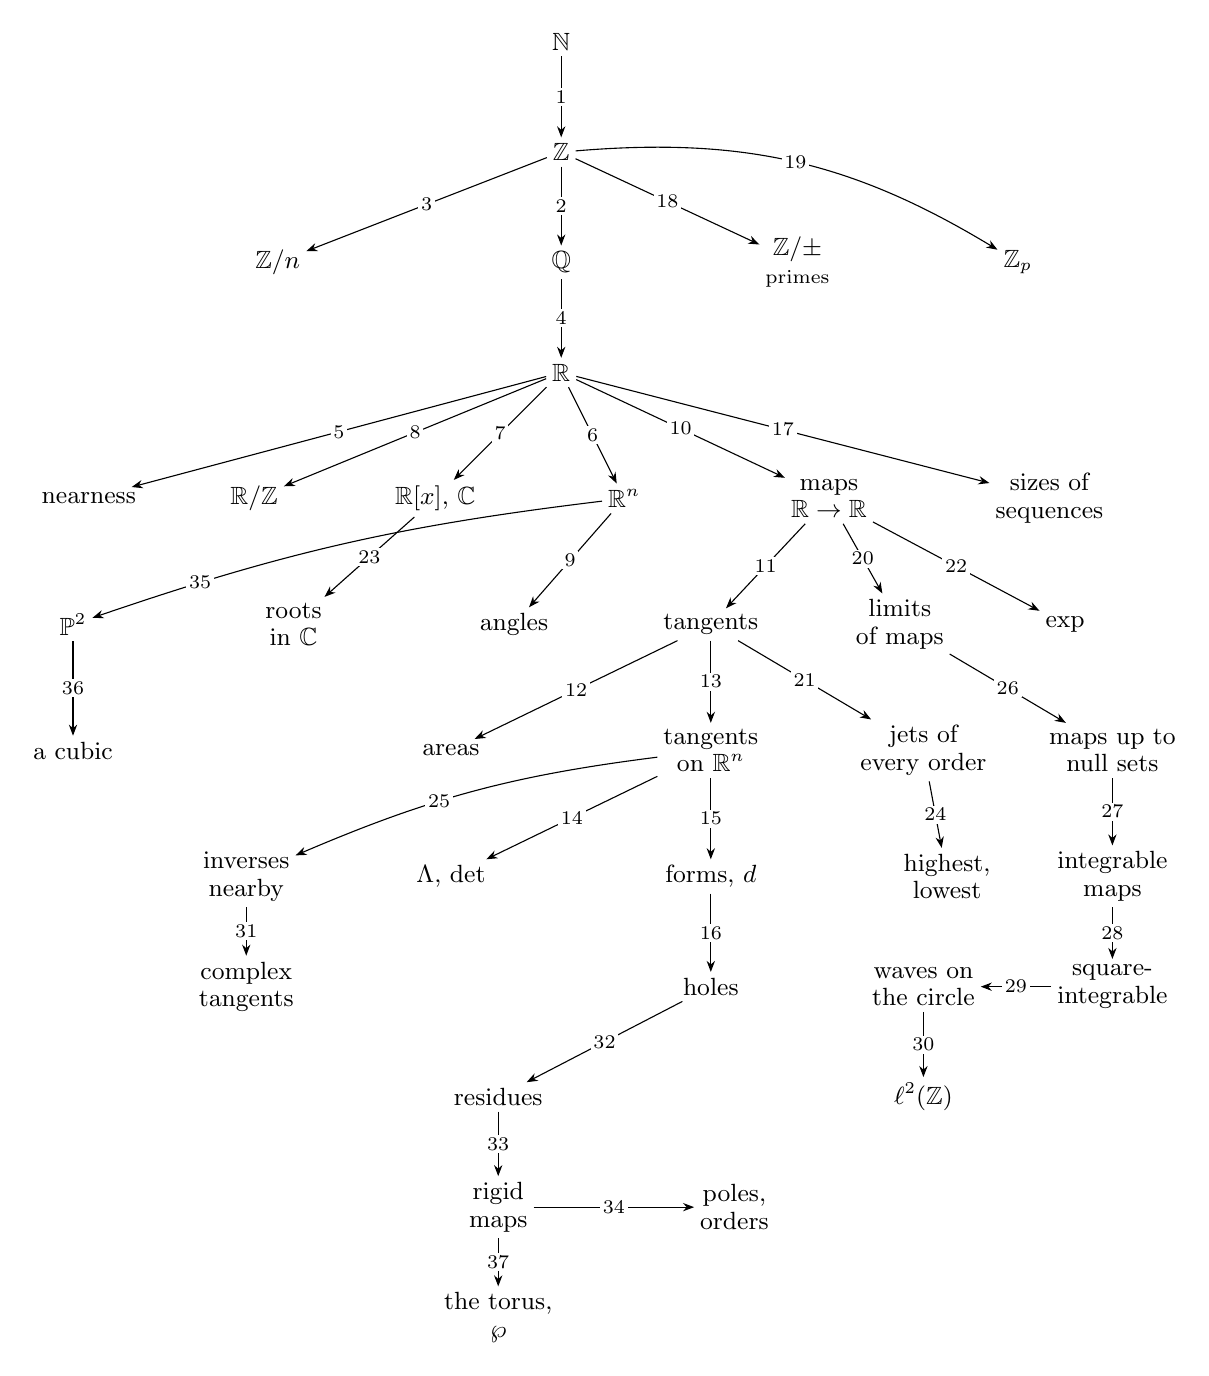
\begin{tikzpicture}[
    x=1cm, y=1cm,
    sys/.style={font=\small, inner sep=2pt, align=center},
    ch/.style={font=\scriptsize, fill=white, inner sep=1pt},
    ar/.style={-{Stealth[length=4pt]}, thin}]
  % numbers
  \node[sys] (N)   at (0, 0)      {$\N$};
  \node[sys] (Z)   at (0,-1.4)    {$\Z$};
  \node[sys] (Zn)  at (-3.6,-2.8) {$\Z/n$};
  \node[sys] (Q)   at (0,-2.8)    {$\Q$};
  \node[sys] (Zpm) at (3.0,-2.8)  {$\Z/{\pm}$\\[-1pt]{\scriptsize primes}};
  \node[sys] (Zp)  at (5.8,-2.8)  {$\Z_p$};
  \node[sys] (R)   at (0,-4.2)    {$\R$};
  % from the reals
  \node[sys] (Nr)  at (-6.0,-5.8) {nearness};
  \node[sys] (T)   at (-3.9,-5.8) {$\R/\Z$};
  \node[sys] (Rx)  at (-1.6,-5.8) {$\R[x]$, $\mathbb{C}$};
  \node[sys] (Rn)  at (0.8,-5.8)  {$\R^n$};
  \node[sys] (F)   at (3.4,-5.8)  {maps\\[-1pt]$\R \to \R$};
  \node[sys] (Sz)  at (6.2,-5.8)  {sizes of\\[-1pt]sequences};
  % next level
  \node[sys] (Rt)  at (-3.4,-7.4) {roots\\[-1pt]in $\mathbb{C}$};
  \node[sys] (An)  at (-0.6,-7.4) {angles};
  \node[sys] (Tg)  at (1.9,-7.4)  {tangents};
  \node[sys] (Lm)  at (4.3,-7.4)  {limits\\[-1pt]of maps};
  \node[sys] (Ex)  at (6.4,-7.4)  {$\exp$};
  % calculus
  \node[sys] (Ar)  at (-1.4,-9.0) {areas};
  \node[sys] (Sv)  at (1.9,-9.0)  {tangents\\[-1pt]on $\R^n$};
  \node[sys] (Jt)  at (4.6,-9.0)  {jets of\\[-1pt]every order};
  \node[sys] (Hi)  at (4.9,-10.6) {highest,\\[-1pt]lowest};
  \node[sys] (Iv)  at (-4.0,-10.6){inverses\\[-1pt]nearby};
  \node[sys] (La)  at (-1.4,-10.6){$\Lambda$, $\det$};
  \node[sys] (Fm)  at (1.9,-10.6) {forms, $d$};
  \node[sys] (Hl)  at (1.9,-12.0) {holes};
  \node[sys] (Nu)  at (7.0,-9.0)  {maps up to\\[-1pt]null sets};
  \node[sys] (Lo)  at (7.0,-10.6) {integrable\\[-1pt]maps};
  \node[sys] (Lt)  at (7.0,-12.0) {square-\\[-1pt]integrable};
  \node[sys] (Wv)  at (4.6,-12.0) {waves on\\[-1pt]the circle};
  \node[sys] (Lz)  at (4.6,-13.4) {$\ell^2(\Z)$};
  \node[sys] (Ct)  at (-4.0,-12.0) {complex\\[-1pt]tangents};
  \node[sys] (Rs)  at (-0.8,-13.4) {residues};
  \node[sys] (Rg)  at (-0.8,-14.8) {rigid\\[-1pt]maps};
  \node[sys] (Po)  at (2.2,-14.8) {poles,\\[-1pt]orders};
  \node[sys] (Pr)  at (-6.2,-7.4) {$\mathbb{P}^2$};
  \node[sys] (Cu)  at (-6.2,-9.0) {a cubic};
  \node[sys] (To)  at (-0.8,-16.2) {the torus,\\[-1pt]$\wp$};
  % arrows, labelled by chapter
  \draw[ar] (N)  -- node[ch]{1}  (Z);
  \draw[ar] (Z)  -- node[ch]{2}  (Q);
  \draw[ar] (Z)  -- node[ch]{3}  (Zn);
  \draw[ar] (Z)  -- node[ch]{18} (Zpm);
  \draw[ar] (Z)  to[bend left=18] node[ch]{19} (Zp);
  \draw[ar] (Q)  -- node[ch]{4}  (R);
  \draw[ar] (R)  -- node[ch]{5}  (Nr);
  \draw[ar] (R)  -- node[ch]{8}  (T);
  \draw[ar] (R)  -- node[ch]{7}  (Rx);
  \draw[ar] (R)  -- node[ch]{6}  (Rn);
  \draw[ar] (R)  -- node[ch]{10} (F);
  \draw[ar] (R)  -- node[ch]{17} (Sz);
  \draw[ar] (Rn) -- node[ch]{9}  (An);
  \draw[ar] (F)  -- node[ch]{11} (Tg);
  \draw[ar] (F)  -- node[ch]{20} (Lm);
  \draw[ar] (F)  -- node[ch]{22} (Ex);
  \draw[ar] (Rx) -- node[ch]{23} (Rt);
  \draw[ar] (Jt) -- node[ch]{24} (Hi);
  \draw[ar] (Sv) to[bend right=8] node[ch, pos=0.6]{25} (Iv);
  \draw[ar] (Tg) -- node[ch]{12} (Ar);
  \draw[ar] (Tg) -- node[ch]{13} (Sv);
  \draw[ar] (Tg) -- node[ch]{21} (Jt);
  \draw[ar] (Sv) -- node[ch]{14} (La);
  \draw[ar] (Sv) -- node[ch]{15} (Fm);
  \draw[ar] (Fm) -- node[ch]{16} (Hl);
  \draw[ar] (Lm) -- node[ch]{26} (Nu);
  \draw[ar] (Nu) -- node[ch]{27} (Lo);
  \draw[ar] (Lo) -- node[ch]{28} (Lt);
  \draw[ar] (Lt) -- node[ch]{29} (Wv);
  \draw[ar] (Wv) -- node[ch]{30} (Lz);
  \draw[ar] (Iv) -- node[ch]{31} (Ct);
  \draw[ar] (Hl) -- node[ch]{32} (Rs);
  \draw[ar] (Rs) -- node[ch]{33} (Rg);
  \draw[ar] (Rg) -- node[ch]{34} (Po);
  \draw[ar] (Rn) to[bend right=6] node[ch, pos=0.8]{35} (Pr);
  \draw[ar] (Pr) -- node[ch]{36} (Cu);
  \draw[ar] (Rg) -- node[ch]{37} (To);
\end{tikzpicture}
\end{center}

Every arrow puts the old numbers \emph{inside} the new ones, except Chapters 3, 8 and 18, which make \emph{pictures} of the old numbers. The tree shows only the main parent of each chapter; the ``from'' line under each chapter title lists all of them.

% ---------------------------------------------------------------
% One row per chapter. p-columns wrap long entries; longtable lets
% the table run onto the next page instead of being cut off.
% ---------------------------------------------------------------
{\small
\renewcommand{\arraystretch}{1.25}
\setlength{\tabcolsep}{4pt}
\begin{longtable}{@{}>{\raggedright\arraybackslash}p{3.2cm}
                     >{\raggedright\arraybackslash}p{2.2cm}
                     >{\raggedright\arraybackslash}p{2.9cm}
                     >{\raggedright\arraybackslash}p{3.2cm}
                     >{\raggedright\arraybackslash}p{2.6cm}@{}}
\textbf{Chapter} & \textbf{Verbs} & \textbf{Forget} & \textbf{Appears} & \textbf{Dies} \\ \hline
\endhead
1. $\N \to \Z$ & build, blur & $(a,b) \sim (a+1,\,b+1)$ & inverses for $+$ & what you had \\
2. $\Z \to \Q$ & build, select, blur & $(a,b) \sim (ac,\,bc)$ & inverses for $\times$ & place-by-place sum \\
3. $\Z \to \Z/n$ & blur & $n \sim 0$ & finite arithmetic & the order $\le$ \\
4. $\Q \to \R$ & build, select, blur & fading $\sim 0$ & limits, $\sqrt{2}$ & every single term \\
5. cells of $\R \to$ likenesses & blur, picture & which cell & nearness; $\varepsilon$--$\delta$ & chaining \\
6. $\R \to \R^n$ & build & nothing & room, dimension & (not carried: $\le$) \\
7. $\R \to \R[x]$ & build, blur & the laws & a free letter; $\mathbb{C}$ & how it was written \\
8. $\R \to \R/\Z$ & blur & $1 \sim 0$ & angles & $\times$ and $\le$ \\
9. corners $\to$ angles & build, select, blur & turns, stretches & $\cos$, $\sin$ & lengths \\
10. $\R \to$ maps & build, select, blur & all but near $a$ & germs; $\pi$; $\mathbb{T} = S$ & far values \\
11. germs $\to$ tangents & blur, select & what is flat & the slope $f'(a)$ & bending \\
12. maps $\to$ areas & select, blur & the constant & $\int_b^c f = F(c) - F(b)$ & the value $F(b)$ \\
13. maps on $\R^n \to$ tangents & build, select, blur & what is flat & covectors $df$ & slices alone \\
14. words in arrows $\to$ $\Lambda$ & build, blur & $v \wedge v \sim 0$ & $\det$, area, volume & order of factors \\
15. $k$-forms $\to$ $(k{+}1)$-forms & select & nothing chosen (blur of $d$, W4) & $d$, with $d \circ d = 0$ & constants \\
16. closed forms $\to$ holes & build, blur & every $df$ & $H^1$: the holes & values at a point \\
17. sequences $\to$ sizes & build, select, blur & constant factors & the scale $1, L(n), n, 2^n, \dots$ & subtraction \\
18. $\Z$ under $\times \to$ division & one-way blur, blur & $-1 \sim 1$ & primes; $\mid$ kept by the $v_p$ & the sign, $+$, $\le$ \\
19. $\Z \to \Z_p$ & ladder, build, select, blur & what comes near $0$ & digits to the left, one per bag & size, sign, $\le$ \\
20. maps $\to$ limits of maps & build, select, blur & what comes near $0$ in $M$ & nothing new: $C[b,c]$ closed & continuity, $\int$ point by point \\
21. germs $\to$ jets & ladder, select & flat to order $k$ & Taylor polynomial; $\R[x]/x^{k+1}$ & the next coefficient; the germ \\
22. maps $\to$ the one with $f' = f$ & select & nothing chosen (blur of $E_c$, W4) & $\exp$, with its law from ``only one'' & the construction \\
23. polynomials over $\mathbb{C}$ $\to$ roots & survives, dies & all but the first two terms at a point & nothing new: $\mathbb{C}$ is closed & $k$-th roots over $\R$ \\
24. maps on $\R^n$ $\to$ highest and lowest points & blur & flat to order $2$ at a point & value, covector, quadratic part & the answer, when $Q$ is $0$ in some direction \\
25. maps $\R^n \to \R^n$ $\to$ inverses nearby & select & nothing new (tangent blur of 13) & the inverse, with tangent $(DF)^{-1}$ & ``can be inverted'', on a whole bag \\
26. maps on a stretch $\to$ maps up to a null set & blur & differ only on a null set & none; nothing continuous is glued & the value at a point; ``continuous'' \\
27. $C[b,c]$ $\to$ $L^1$ & build, select, blur & difference fades in the mean & integrable maps; length, last & $\times$; the value at a point; ``continuous'' \\
28. $C[b,c]$ $\to$ $L^2$ & build, select, blur & difference fades in the mean square & $\langle\,,\rangle$, right angles, nearest points & $\times$ \\
29. maps on $\mathbb{T}$ $\to$ lists on $\Z$ & survey, arrow, ladder & nothing new (questions $\widehat f(n)$) & every arrow $\mathbb{T} \to S$; the average of rungs comes back & $\times$ (becomes convolution); one rung overshoots \\
30. $L^2(\mathbb{T})$ $\to$ $\ell^2(\Z)$ & arrow & nothing (an inside) & a matching keeping energy; $\sum 1/n^2 = \pi^2/6$ & the value at a point; ``continuous'' \\
31. maps $\mathbb{C} \to \mathbb{C}$ $\to$ holomorphic & blur, select & flat at $a$ (Chapter 11 over $\mathbb{C}$) & tangent commutes with $i$; angles kept & angles, where $f' = 0$ \\
32. holomorphic maps $\to$ closed $f\,dz$ & arrow & nothing new (Chapter 16's blur) & Cauchy; the residue as a normal form & loop integrals, for $\bar z$; ``no hole'' \\
33. holomorphic maps $\to$ germs & blur & nothing (the germ blur is equality) & power series; Liouville; highest point only on the edge & rigidity, without ``one piece'' \\
34. germs at $a$ $\to$ their order & blur, build & rungs $\operatorname{ord}(f - g) \ge k$ & $\operatorname{ord}_a$, the twin of $v_p$; poles; residues add; zeros counted by turns & ``has an order'' ($\exp(1/z)$) \\
35. $k^3$ without $0$ $\to$ its lines & blur & the size, $v \sim \lambda v$ & $\mathbb{P}^2$: a point known by its lines; no parallels & the value $F(v)$ \\
36. polynomials $\to$ functions on a cubic & build, blur & $y^2 \sim x^3 + ax + b$ & the third point on a line; weights, the twin of $\operatorname{ord}$ & weight $1$; smoothness, when $\Delta = 0$ \\
37. $\mathbb{C} \to \mathbb{C}/\Lambda$ & blur, select & two periods & the torus; $\wp$, pinned by one double pole; the cubic & $\times$; a single simple pole \\
\end{longtable}
}

\textbf{Axioms.} Only Chapter 1 assumes anything (A1--A6, about $\N$). Every later Given is earned in an earlier chapter.

\textbf{How to read a chapter.} Chapter 0 gives the rules: what may be built, what a blur is, and what each line of a chapter claims.

\textbf{The fork.} Up to $\R$ the path is forced: each chapter closes up something missing. Chapter 5 adds no numbers: it finds nearness on $\R$, and every later chapter on limits cites it. After $\R$ the map branches: Chapter 6 builds lists, Chapter 7 builds words, Chapter 8 only blurs. Chapter 9 starts from $\R^2$ and uses the product of Chapter 7; it reaches angles a second way. Chapter 10 builds all maps and shows the two ways meet; Chapter 11 blurs them down to their tangents, and Chapter 12 finds area as the one rule with four properties. Chapters 13 to 16 carry this to several variables and forms, and end by measuring holes. Chapter 17 sorts sequences by size. Chapters 18 and 19 return to $\Z$: divisibility is a one-way blur, and the ladder mod $p^k$ is a nearness whose rungs chain, closing $\Z$ up to $\Z_p$. Chapter 20 puts two nearnesses on maps and finds what survives a limit; Chapter 21 is the ladder of Chapter 11 at every order, the twin of Chapter 19. Chapter 22 selects $\exp$ by what it must do, and so pays what Chapter 10 owed. Chapter 23 goes back to Chapter 7 and shows that gluing $x^2 \sim -1$ was enough: every polynomial has a root in $\mathbb{C}$. Chapter 24 takes the ladder of Chapter 21 to rung $2$ on $\R^n$ and reads highest and lowest points off it. Chapter 25 asks the tangent of Chapter 13 whether a map can be inverted nearby.

\textbf{Part II.} Its Chapter 1 goes one level up: its things are the systems $\N$, $\Z$, $\Z/n$, $\Q$, $\R$, $\R^n$ themselves, and its tests are the laws they pass. There the words \emph{ring}, \emph{field} and \emph{complete} appear, and Part II opens with its own map, of the second floor.

\newpage

%% ==================================================================
%%  Chapter 1  (ch1-integers)
%% ==================================================================
\section*{Chapter 1. The integers}
\phantomsection\addcontentsline{toc}{section}{\texorpdfstring{Chapter 1. The integers \quad $\N \to \Z$}{Chapter 1. The integers}}
\begin{center}
{\normalsize $\N \to \Z$ \quad$\cdot$\quad from: the axioms \quad$\cdot$\quad build, blur}\\[4pt]
{\small Build the debts, then forget their history.}
\end{center}

\subsection*{Axioms}

Given $\N$ with $0$, $1$, $+$, $\times$ such that, for all $a,b,c$ in $\N$:
\begin{lines}
\item[\lab{A1}] $+$ and $\times$ are associative and commutative.
\item[\lab{A2}] $a + 0 = a$ and $a \times 1 = a$.
\item[\lab{A3}] $a \times (b + c) = a \times b + a \times c$.
\item[\lab{A4}] $a + c = b + c \;\Rightarrow\; a = b$.
\item[\lab{A5}] $a + 1 \neq 0$.
\item[\lab{A6}] (Induction.) If a set $S \subseteq \N$ holds $0$, and holds $a+1$ whenever it holds $a$, then $S = \N$.
\end{lines}

\subsection*{Definitions}

\begin{lines}
\item[\lab{D0}] For $a,b$ in $\N$: \quad $a \le b \;\iff\; a + c = b$ for some $c$ in $\N$.
\item[\lab{D1}] (Build, M1.) Let $\PP := \N \times \N$. Read $(a,b)$ as ``had $a$, owe $b$''.
\item[\lab{D2}] $(a,b) + (c,d) := (a+c,\; b+d)$.
\item[\lab{D3}] $(a,b) \le (c,d) \;\iff\; a + d \le b + c$.
\item[\lab{D4}] $\sett(a,b) \;\iff\; a = b$.
\end{lines}

\subsection*{Blur}

\begin{lines}
\item[\lab{B1}] (From below, L5.) Gluings: $(a,b) \sim (a+1,\, b+1)$ for all $a, b$ in $\N$. \ Respects: $+$. \ Call this blur $\sim$.
\item[\lab{B2}] (From above, L6.) Question: $\sett$. \ Respects: $+$. \ Call this blur $\approx$. \\
By Z3: \ $x \approx y \iff \bigl(\sett(x+z) \iff \sett(y+z)\bigr)$ for every $z$ in $\PP$.
\item[] A \emph{bag} is a bag of $\sim$ (L1). Write $\bag{a,b}$ for the bag of $(a,b)$.
\end{lines}

\subsection*{Propositions}

\begin{lines}
\item[\lab{P1}] (Bags.) $(a,b) \sim (c,d) \;\iff\; a + d = b + c$.
\item[\lab{P2}] (Normal forms.) Each bag holds exactly one pair of the form $(n,0)$ or $(0,n)$.
\item[\lab{P3.1}] ($+$ survives.) If $x \sim x'$ and $y \sim y'$ then $x + y \sim x' + y'$.
\item[\lab{P3.2}] ($\le$ survives.) If $x \sim x'$ and $y \sim y'$ then $x \le y \iff x' \le y'$.
\item[\lab{P3.3}] ($\sett$ survives.) If $x \sim x'$ then $\sett(x) \iff \sett(x')$.
\item[\lab{P4}] (``Had'' dies.) The map $(a,b) \mapsto a$ is not constant on bags: $(3,5) \sim (4,6)$ but $3 \neq 4$.
\item[\lab{P5}] (Appears.) The two blurs agree: $\;\sim \;=\; \approx$. \ (By Z4 and Z5; the separating context is $z = (b,a)$, the swap of $x = (a,b)$.) \\
So $\sim$ is exactly the blur at which the question ``is $x + z$ settled?'' lives.
\end{lines}

\subsection*{Notation}

\begin{lines}
\item[\lab{N1}] Let $\Z := \{\text{bags}\} = \PP/{\sim}$ (M5), with $+$ and $\le$ carried over by P3.1 and P3 (Z6).2.
\item[\lab{N2}] Let $0 := \bag{0,0}$, and for $n$ in $\N$ let $\;n := \bag{n,0}$, $\;-n := \bag{0,n}$.
\end{lines}

\subsection*{Arrow}

\begin{lines}
\item[\lab{P6}] The map $\N \to \Z$, $n \mapsto \bag{n,0}$, is one-to-one and respects $0$, $+$ and $\le$. \\
This is what allows the letter $n$ to be reused in N2.
\end{lines}

\subsection*{Theorems}

\begin{lines}
\item[\lab{T1}] (Inverses.) For every $x$ in $\Z$ there is exactly one $y$ in $\Z$ with $x + y = 0$. If $x = \bag{a,b}$ then $y = \bag{b,a}$.
\item[\lab{T2}] (Total order.) For all $x,y$ in $\Z$: $x \le y$ or $y \le x$; and if both, then $x = y$.
\item[\lab{T3}] (Shape.) Every $x$ in $\Z$ is $n$ or $-n$ for exactly one $n$ in $\N$, and $n = -n$ only for $n = 0$.
\end{lines}

\subsection*{Remarks}

\begin{lines}
\item[\lab{R1}] (Forgetting the sign.) The smallest blur with $(a,b) \sim (b,a)$ that respects $+$ also glues $2$ to $0$. It gives parity, $\Z/2$, not ``integers without sign''.
\item[\lab{R2}] (Clocks.) The smallest blur with $(n,0) \sim (0,0)$ that respects $+$ gives $\Z/n$.
\item[\lab{R3}] (Sign and size.) By P2, $\Z$ can be stored as $\{0,1\} \times \N$ with the two zeros glued. Then $+$ must be computed by cases.
\end{lines}

\begin{lines}
\item[\lab{R4}] (Shared signs.) $+$ names three operations: on $\N$, on $\PP$ (D2), and on $\Z$ (N1). P3.1 lets the second descend to the third; P6 shows the third agrees with the first.
\end{lines}

\subsection*{Exercises}

\begin{lines}
\item[\lab{E1}] Define $(a,b) \times (c,d) := (ac + bd,\; ad + bc)$. Show that $\times$ survives.
\item[\lab{E2}] Show that in $\Z$: if $x \times y = 0$ then $x = 0$ or $y = 0$. (The next chapter needs this.)
\item[\lab{E3}] Show that in $\Z$, $+$ and $\times$ are associative and commutative, $0$ and $1$ are neutral, and $\times$ distributes over $+$. (For $+$, use Z7. For $\times$, check on $\PP$ first.)
\item[\lab{E4}] Show that in $\Z$: $x \le y \Rightarrow x + z \le y + z$, and $0 \le x,\ 0 \le y \Rightarrow 0 \le x \times y$.
\item[\lab{E5}] Show that every non-empty set of integers $x > 0$ has a least element.
\item[\lab{E6}] Show that A1--A4 and A6 without A5 are satisfied by a clock with five elements, and find where P2 then fails.
\end{lines}

\newpage

%% ==================================================================
%%  Chapter 2  (ch2-rationals)
%% ==================================================================
\section*{Chapter 2. The rationals}
\phantomsection\addcontentsline{toc}{section}{\texorpdfstring{Chapter 2. The rationals \quad $\Z \to \Q$}{Chapter 2. The rationals}}
\begin{center}
{\normalsize $\Z \to \Q$ \quad$\cdot$\quad from: Chapter 1 \quad$\cdot$\quad build, select, blur}\\[4pt]
{\small Build the shares, select the possible ones, then forget their scale.}
\end{center}

\subsection*{Given}

Given $\Z$ with $0$, $1$, $+$, $-$, $\times$, $\le$ such that, for all $x,y,z$ in $\Z$:
\begin{lines}
\item[\lab{G1}] $+$ and $\times$ are associative and commutative.
\item[\lab{G2}] $x + 0 = x$ and $x \times 1 = x$, and $0 \neq 1$.
\item[\lab{G3}] $x \times (y + z) = x \times y + x \times z$.
\item[\lab{G4}] $x + (-x) = 0$.
\item[\lab{G5}] $x \times y = 0 \;\Rightarrow\; x = 0$ or $y = 0$.
\item[\lab{G6}] $\le$ is a total order.
\item[\lab{G7}] $x \le y \Rightarrow x + z \le y + z$; \quad and $0 \le x,\ 0 \le y \Rightarrow 0 \le x \times y$.
\item[\lab{G8}] Every non-empty set of integers $x > 0$ has a least element.
\end{lines}
Nothing here is assumed. Each line is a theorem or an exercise of Chapter 1 (G1--G3 are E3, G4 is T1, G5 is E2, G6 is T2, G7 is E4, G8 is E5).

\subsection*{Definitions}

\begin{lines}
\item[\lab{D1}] (Build, M1.) Let $\Z \times \Z$ be the pairs. Read $(a,b)$ as ``$a$ shared among $b$''.
\item[\lab{D2}] (Select, M4.) Let $\FF := \{(a,b) \in \Z \times \Z : b \neq 0\}$.
\item[\lab{D3}] $(a,b) \times (c,d) := (ac,\; bd)$.
\item[\lab{D4}] $(a,b) + (c,d) := (ad + bc,\; bd)$.
\item[\lab{D5}] $(a,b) \le (c,d) \;\iff\; (ab)(dd) \le (cd)(bb)$.
\item[\lab{D6}] $\whole(a,b) \;\iff\; a = b$.
\end{lines}
By G5, $\FF$ is closed under D3 and D4.

\subsection*{Blur}

\begin{lines}
\item[\lab{B1}] (From below, L5.) Gluings: $(a,b) \sim (ac,\, bc)$ for all $(a,b)$ in $\FF$ and all $c \neq 0$. \ Respects: $\times$. \ Call this blur $\sim$.
\item[\lab{B2}] (From above, L6.) Question: $\whole$. \ Respects: $\times$. \ Call this blur $\approx$. \\
By Z3: \ $x \approx y \iff \bigl(\whole(x \times z) \iff \whole(y \times z)\bigr)$ for every $z$ in $\FF$.
\item[] A \emph{bag} is a bag of $\sim$ (L1). Write $\bag{a,b}$ for the bag of $(a,b)$.
\end{lines}

\subsection*{Propositions}

\begin{lines}
\item[\lab{P1}] (Bags.) $(a,b) \sim (c,d) \;\iff\; ad = bc$.
\item[\lab{P2}] (Normal forms.) Each bag holds exactly one pair $(a,b)$ with $b > 0$ and $b$ least.
\item[\lab{P3.1}] ($\times$ survives.) If $x \sim x'$ and $y \sim y'$ then $x \times y \sim x' \times y'$.
\item[\lab{P3.2}] ($+$ survives.) If $x \sim x'$ and $y \sim y'$ then $x + y \sim x' + y'$.
\item[\lab{P3.3}] ($\le$ survives.) If $x \sim x'$ and $y \sim y'$ then $x \le y \iff x' \le y'$.
\item[\lab{P3.4}] ($\whole$ survives.) If $x \sim x'$ then $\whole(x) \iff \whole(x')$.
\item[\lab{P4.1}] (``Top'' dies.) The map $(a,b) \mapsto a$ is not constant on bags: $(1,2) \sim (2,4)$ but $1 \neq 2$.
\item[\lab{P4.2}] (Place-by-place sum dies.) Let $(a,b) \oplus (c,d) := (a+c,\; b+d)$. Then $(1,2) \sim (2,4)$, but
$(1,2) \oplus (1,3) = (2,5)$ and $(2,4) \oplus (1,3) = (3,7)$ are not in one bag, since $2 \times 7 \neq 5 \times 3$.
\item[\lab{P5}] (Appears.) The two blurs agree: $\;\sim \;=\; \approx$. \ (By Z4 and Z5; the separating context is $z = (b,a)$, the swap of $x = (a,b)$, when $a \neq 0$.) \\
So $\sim$ is exactly the blur at which the question ``is $x \times z$ whole?'' lives.
\end{lines}

\subsection*{Notation}

\begin{lines}
\item[\lab{N1}] Let $\Q := \{\text{bags}\} = \FF/{\sim}$ (M5), with $\times$, $+$, $\le$ carried over by P3.1--P3 (Z6).3.
\item[\lab{N2}] Let $\dfrac{a}{b} := \bag{a,b}$, and for $a$ in $\Z$ let $a := \bag{a,1}$.
\end{lines}

\subsection*{Arrow}

\begin{lines}
\item[\lab{P6}] The map $\Z \to \Q$, $a \mapsto \bag{a,1}$, is one-to-one and respects $0$, $1$, $+$, $\times$ and $\le$. \\
This is what allows the letter $a$, and the signs $+$, $\times$, $\le$, to be reused in N2.
\end{lines}

\subsection*{Theorems}

\begin{lines}
\item[\lab{T1}] (Inverses.) For every $x \neq 0$ in $\Q$ there is exactly one $y$ in $\Q$ with $x \times y = 1$. If $x = \bag{a,b}$ then $y = \bag{b,a}$.
\item[\lab{T2}] (Zero has none.) There is no $y$ in $\Q$ with $0 \times y = 1$.
\item[\lab{T3}] (Field.) G1--G5 hold in $\Q$. (G1--G4 are equations; G5 is not, and must be checked: Z7, Z8.)
\item[\lab{T4}] (Order.) G6 and G7 hold in $\Q$.
\item[\lab{T5}] (Division.) For $a, b$ in $\Z$ with $b \neq 0$, the equation $b \times x = a$ has exactly one solution in $\Q$, namely $\dfrac{a}{b}$.
\item[\lab{T6}] (Density.) If $x < y$ in $\Q$ then there is $z$ in $\Q$ with $x < z < y$.
\item[\lab{T7}] (G8 is lost.) The set of $x > 0$ in $\Q$ has no least element.
\end{lines}

\subsection*{Remarks}

\begin{lines}
\item[\lab{R1}] (Why Select.) Without D2, the blur B1 on all of $\Z \times \Z$ has two extra bags, $\bag{1,0}$ and $\bag{0,0}$. Then P1 fails: the test $ad = bc$ is no longer transitive, and closing it glues every pair to $(0,0)$. G4 fails too: $\bag{1,0} + y$ is never $0$. Select removes exactly the pairs that break the laws.
\item[\lab{R2}] (Same chapter twice.) Chapter 1 is this chapter with $+$ in place of $\times$: pairs, a gluing ``do the same to both places'', the swap as inverse, $\operatorname{sett}$ in place of $\whole$. The one difference is D2: in $\N$ every $c$ cancels under $+$ (A4), in $\Z$ only $c \neq 0$ cancels under $\times$ (G5).
\item[\lab{R3}] (Smaller selections.) Selecting only $b$ a power of $2$, or only $b$ a power of $10$, gives smaller number systems between $\Z$ and $\Q$ (the binary and the decimal fractions). Select is a choice, as Blur is.
\item[\lab{R4}] (Shared signs.) $+$ names three operations: on $\Z$, on $\FF$ (D4), and on $\Q$ (N1). P3.2 lets the second descend to the third; P6 shows the third agrees with the first.
\end{lines}

\subsection*{Exercises}

\begin{lines}
\item[\lab{E1}] D4 is not done place by place. Show that it is forced: it is the only choice for which P6 respects $+$ and T3 holds.
\item[\lab{E2}] Prove R1.
\item[\lab{E3}] Show there is no $x$ in $\Q$ with $x \times x = 2$. (The chapter on the real numbers starts here.)
\item[\lab{E4}] In R3 with $b$ a power of $2$: which of T1--T7 still hold?
\item[\lab{E5}] Show that for every $x$ in $\Q$ there is $n$ in $\N$ with $x < n$. (Chapter 4 needs this.)
\end{lines}

\newpage

%% ==================================================================
%%  Chapter 3  (ch3-congruences)
%% ==================================================================
\section*{Chapter 3. Congruences}
\phantomsection\addcontentsline{toc}{section}{\texorpdfstring{Chapter 3. Congruences \quad $\Z \to \Z/n$}{Chapter 3. Congruences}}
\begin{center}
{\normalsize $\Z \to \Z/n$ \quad$\cdot$\quad from: Chapter 1 \quad$\cdot$\quad blur}\\[4pt]
{\small Build nothing. Forget how many times round.}
\end{center}

\subsection*{Given}

Given $\Z$ with $0$, $1$, $+$, $-$, $\times$, $\le$ and the laws G1--G8 of Chapter 2 (all earned in Chapter 1).

\subsection*{Definitions}

\begin{lines}
\item[\lab{D1}] Let $n$ in $\Z$ with $n > 0$, fixed for the whole chapter.
\item[\lab{D2}] $\mult(x) \;\iff\; x = n \times k$ for some $k$ in $\Z$. \quad (``$x$ is a multiple of $n$''.)
\end{lines}
There is no Build line. The floor is $\Z$ itself, with $O = \{+, -, \times\}$.

\subsection*{Blur}

\begin{lines}
\item[\lab{B1}] (From below, L5.) Gluings: the single pair $n \sim 0$. \ Respects: $+$. \ Call this blur $\sim$.
\item[\lab{B2}] (From above, L6.) Question: $\mult$. \ Respects: $+$. \ Call this blur $\approx$. \\
By Z3: \ $x \approx y \iff \bigl(\mult(x+z) \iff \mult(y+z)\bigr)$ for every $z$ in $\Z$.
\item[] A \emph{bag} is a bag of $\sim$ (L1). Write $\bag{x}$ for the bag of $x$.
\end{lines}

\subsection*{Propositions}

\begin{lines}
\item[\lab{P1}] (Bags.) $x \sim y \;\iff\; \mult(x - y)$.
\item[\lab{P2}] (Normal forms.) Each bag holds exactly one $r$ with $0 \le r < n$. So there are exactly $n$ bags.
\item[\lab{P3.1}] ($+$ survives.) If $x \sim x'$ and $y \sim y'$ then $x + y \sim x' + y'$.
\item[\lab{P3.2}] ($-$ survives.) If $x \sim x'$ then $-x \sim -x'$.
\item[\lab{P3.3}] ($\times$ survives.) If $x \sim x'$ and $y \sim y'$ then $x \times y \sim x' \times y'$. \\
B1 did not ask for this. It comes free.
\item[\lab{P3.4}] ($\mult$ survives.) If $x \sim x'$ then $\mult(x) \iff \mult(x')$.
\item[\lab{P4}] ($\le$ dies, for $n \ge 2$.) $0 \sim n$ and $1 \sim 1$, and $0 \le 1$, but not $n \le 1$.
\item[\lab{P5}] (Appears.) The two blurs agree: $\;\sim \;=\; \approx$. \ (By Z4 and Z5; the separating context is $z = -x$.) \\
So $\sim$ is exactly the blur at which the question ``is $x + z$ a multiple of $n$?'' lives.
\end{lines}

\subsection*{Notation}

\begin{lines}
\item[\lab{N1}] Let $\Zn := \{\text{bags}\} = \Z/{\sim}$ (M5), with $+$, $-$, $\times$ carried over by P3.1--P3.3 (Z6).
\item[\lab{N2}] Write $x \equiv y \pmod n$ for $x \sim y$.
\end{lines}

\subsection*{Arrow}

\begin{lines}
\item[\lab{P6}] The map $\Z \to \Zn$, $x \mapsto \bag{x}$, respects $0$, $1$, $+$, $-$, $\times$, and reaches every bag. It is not one-to-one. \\
In Chapters 1 and 2 the arrow put the old numbers \emph{inside} the new ones. Here the arrow \emph{is} the blur: the new numbers are a picture of the old.
\end{lines}

\subsection*{Theorems}

\begin{lines}
\item[\lab{T1}] (Ring.) G1, G3, G4 hold in $\Zn$, and $x + \bag{0} = x$, $x \times \bag{1} = x$. (All equations: free by Z7.)
\item[\lab{T2}] (No order.) For $n \ge 2$ there is no total order on $\Zn$ with $x \le y \Rightarrow x + z \le y + z$.
\item[\lab{T3}] (Inverses.) $\bag{a}$ has a $y$ in $\Zn$ with $\bag{a} \times y = \bag{1}$ if and only if the only $d > 0$ dividing both $a$ and $n$ is $1$.
\item[\lab{T4}] (Primes.) G5 holds in $\Zn$ if and only if $n$ is prime. In that case every $x \neq \bag{0}$ has an inverse.
\item[\lab{T5}] (Fermat.) If $n$ is prime then $x^n = x$ for every $x$ in $\Zn$.
\item[\lab{T6}] (Two clocks.) If the only $d > 0$ dividing both $m$ and $n$ is $1$, then $\bag{x}_{mn} \mapsto (\bag{x}_m, \bag{x}_n)$ is one-to-one from $\Z/mn$ onto $\Z/m \times \Z/n$, and respects $+$ and $\times$.
\end{lines}

\subsection*{Remarks}

\begin{lines}
\item[\lab{R1}] (The whole map.) Every blur of $\Z$ that respects $+$ is the blur of this chapter for exactly one $n \ge 0$, where $n = 0$ means ``nothing glued'' and $n = 1$ means ``one bag''. The blur for $m$ is blurrier than the blur for $n$ exactly when $m$ divides $n$. So this chapter lists every way to blur $\Z$, and divisibility is the order on the list.
\item[\lab{R2}] (Parity.) $n = 2$ is the parity chapter, and Remark R1 of Chapter 1.
\item[\lab{R3}] (Three shapes.) Chapter 1: build, blur. Chapter 2: build, select, blur. Chapter 3: blur only.
\item[\lab{R4}] (One-way blurs.) A blur glues both ways. A \emph{one-way blur} only orders: a relation $x \preceq y$, reflexive and transitive, with $x \preceq y \Rightarrow xz \preceq yz$. On $(\Z/6, \times)$ a machine search finds $162$ of them, of which $27$ are partial orders. The general counts are recent work in this project and have not yet been checked by outside readers.
\end{lines}

\subsection*{Exercises}

\begin{lines}
\item[\lab{E1}] For $n = 6$: list the bags, and write the tables of $+$ and $\times$.
\item[\lab{E2}] Find every $x$ in $\Z/8$ with $x \times x = \bag{1}$. Compare with $\Z/7$.
\item[\lab{E3}] Prove R1. (Hint: G8.)
\item[\lab{E4}] B1 with ``$x \sim y \Rightarrow x \times z \sim y \times z$'' in place of the $+$ rule: which bags result?
\item[\lab{E5}] Why can $\le$ not be repaired by choosing normal forms (P2) and comparing those? Which half of G7 fails?
\end{lines}

\newpage

%% ==================================================================
%%  Chapter 4  (ch4-reals)
%% ==================================================================
\section*{Chapter 4. The real numbers}
\phantomsection\addcontentsline{toc}{section}{\texorpdfstring{Chapter 4. The real numbers \quad $\Q \to \R$}{Chapter 4. The real numbers}}
\begin{center}
{\normalsize $\Q \to \R$ \quad$\cdot$\quad from: Chapter 2 \quad$\cdot$\quad build, select, blur}\\[4pt]
{\small Build the approximations, select the ones that settle, then forget how they got there.}
\end{center}

\subsection*{Given}

Given $\N$ (Chapter 1) and $\Q$ with $0$, $1$, $+$, $-$, $\times$, $\le$ such that:
\begin{lines}
\item[\lab{G1}] $\Q$ is a field: G1--G4 of Chapter 2 hold, and every $x \neq 0$ has a $y$ with $x \times y = 1$.
\item[\lab{G2}] $\le$ is a total order with $x \le y \Rightarrow x + z \le y + z$, and $0 \le x,\ 0 \le y \Rightarrow 0 \le x \times y$.
\item[\lab{G3}] For every $x$ in $\Q$ there is $n$ in $\N$ with $x < n$.
\end{lines}
Nothing here is assumed (G1 is T1 and T3 of Chapter 2, G2 is T4, G3 is E5).

Throughout, $\varepsilon$ stands for an element of $\Q$ with $\varepsilon > 0$, and $j, k, N$ for elements of $\N$.

\subsection*{Definitions}

\begin{lines}
\item[\lab{D0}] $|x| := x$ if $0 \le x$, and $|x| := -x$ otherwise.
\item[\lab{D1}] (Build, M2.) Let $\Seq$ be the sequences in $\Q$: all maps $a : \N \to \Q$, written $a = (a_0, a_1, a_2, \dots)$. \\ Read $a$ as ``a list of better and better approximations''.
\item[\lab{D2}] $(a + b)_k := a_k + b_k$ \quad and \quad $(a \times b)_k := a_k \times b_k$.
\item[\lab{D3}] (Select, M4.) $a$ \emph{settles} if for every $\varepsilon$ there is $N$ with $|a_j - a_k| < \varepsilon$ for all $j, k \ge N$. \\
Let $\CC := \{a \in \Seq : a \text{ settles}\}$.
\item[\lab{D4}] $\nul(a) \;\iff\;$ for every $\varepsilon$ there is $N$ with $|a_k| < \varepsilon$ for all $k \ge N$. \quad (``$a$ fades''.)
\item[\lab{D5}] $\pos(a) \;\iff\;$ there are $\varepsilon$ and $N$ with $a_k > \varepsilon$ for all $k \ge N$.
\item[\lab{D6}] $a \le b \;\iff\;$ for every $\varepsilon$ there is $N$ with $a_k \le b_k + \varepsilon$ for all $k \ge N$.
\end{lines}
$\CC$ is closed under D2, and every fading sequence settles.

\subsection*{Blur}

\begin{lines}
\item[\lab{B1}] (From below, L5.) Gluings: $e \sim 0$ for every fading $e$ in $\CC$, where $0 = (0, 0, 0, \dots)$. \ Respects: $+$. \ Call this blur $\sim$.
\item[\lab{B2}] (From above, L6.) Question: $\pos$. \ Respects: $+$. \ Call this blur $\approx$. \\
By Z3: \ $a \approx b \iff \bigl(\pos(a+c) \iff \pos(b+c)\bigr)$ for every $c$ in $\CC$.
\item[] A \emph{bag} is a bag of $\sim$ (L1). Write $\bag{a}$ for the bag of $a$.
\end{lines}

\subsection*{Propositions}

\begin{lines}
\item[\lab{P1}] (Bags.) $a \sim b \;\iff\; \nul(a - b)$.
\item[\lab{P2}] (Normal forms.) Each bag holds exactly one \emph{decimal} sequence: one with $a_k = m_k / 10^k$, $m_k$ in $\Z$, and $10\, m_k \le m_{k+1} \le 10\, m_k + 9$ for all $k$, in which $m_{k+1} = 10\, m_k + 9$ does not hold for all large $k$.
\item[\lab{P3.1}] ($+$ survives.) If $a \sim a'$ and $b \sim b'$ then $a + b \sim a' + b'$.
\item[\lab{P3.2}] ($\times$ survives.) If $a \sim a'$ and $b \sim b'$ then $a \times b \sim a' \times b'$.
\item[\lab{P3.3}] ($\le$ survives.) If $a \sim a'$ and $b \sim b'$ then $a \le b \iff a' \le b'$.
\item[\lab{P3.4}] ($\pos$ survives.) If $a \sim a'$ then $\pos(a) \iff \pos(a')$.
\item[\lab{P4.1}] (Every single term dies.) For each $k$, the map $a \mapsto a_k$ is not constant on bags: $(1, 0, 0, \dots) \sim (0, 0, 0, \dots)$.
\item[\lab{P4.2}] (``All terms positive'' dies.) $(1, \tfrac12, \tfrac13, \dots) \sim (0, 0, 0, \dots)$: every term of the first is $> 0$, no term of the second is.
\item[\lab{P5}] (Appears.) The two blurs agree: $\;\sim \;=\; \approx$. \ (By Z4 and Z5; the separating context is $c = -a$ or $c = -b$.) \\
So $\sim$ is exactly the blur at which the question ``is $a + c$ positive in the long run?'' lives.
\end{lines}

\subsection*{Notation}

\begin{lines}
\item[\lab{N1}] Let $\R := \{\text{bags}\} = \CC/{\sim}$ (M5), with $+$, $\times$, $\le$ carried over by P3.1--P3 (Z6).3.
\item[\lab{N2}] For $q$ in $\Q$ let $q := \bag{(q, q, q, \dots)}$.
\item[\lab{N3}] For a sequence $x_0, x_1, \dots$ in $\R$ and $x$ in $\R$, write $x_k \to x$ if for every $\varepsilon$ there is $N$ with $|x_k - x| < \varepsilon$ for all $k \ge N$.
\end{lines}

\subsection*{Arrow}

\begin{lines}
\item[\lab{P6}] The map $\Q \to \R$, $q \mapsto \bag{(q, q, q, \dots)}$, is one-to-one and respects $0$, $1$, $+$, $\times$ and $\le$.
\item[\lab{P7}] (The approximations approximate.) If $a$ is in $\CC$ then $a_k \to \bag{a}$.
\end{lines}

\subsection*{Theorems}

\begin{lines}
\item[\lab{T1}] (Field.) G1 holds in $\R$. (The equations are free by Z7; inverses must be checked, Z8.)
\item[\lab{T2}] (Order.) G2 holds in $\R$.
\item[\lab{T3}] (Archimedes.) G3 holds in $\R$.
\item[\lab{T4}] (Density.) If $x < y$ in $\R$ then there is $q$ in $\Q$ with $x < q < y$.
\item[\lab{T5}] (Square root of two.) There is exactly one $x > 0$ in $\R$ with $x \times x = 2$.
\item[\lab{T6}] (Completeness.) Every sequence in $\R$ that settles has a limit: there is $x$ in $\R$ with $x_k \to x$.
\item[\lab{T7}] (Once is enough.) Run this chapter again with $\R$ as the Given. Then the Arrow P6, from $\R$ to the new bags, is one-to-one \emph{and reaches every bag}. Nothing new appears.
\item[\lab{T8}] (Least upper bound.) Every non-empty set of real numbers that has an upper bound has a least one.
\end{lines}

\subsection*{Remarks}

\begin{lines}
\item[\lab{R1}] (A new Build.) This is the first chapter to build with sequences instead of pairs. Its shape is that of Chapter 2: build, select, blur.
\item[\lab{R2}] (Why Select.) On all of $\Seq$ the product dies: $(1, \tfrac12, \tfrac13, \dots) \sim 0$, but multiplying both by $(1, 2, 3, \dots)$ gives $(1, 1, 1, \dots)$ and $0$, which are not in one bag. Select removes the sequences that break P3.2.
\item[\lab{R3}] (Completeness is a closure.) T7 says the chapter, seen as a machine $\Q \mapsto \R$, gives nothing new when fed its own output. The earlier chapters are the same: pairs of integers under Chapter 1 give $\Z$ again, and fractions of fractions under Chapter 2 give $\Q$ again. Each chapter is a closing-up, and completeness is the name of being closed under this one.
\item[\lab{R4}] (No rule picks the best member.) In Chapters 1--3 the normal form was the smallest member of the bag. Here P2 needs a convention ($0.999\dots$ and $1.000\dots$ share a bag) and an infinite object. This is why real numbers are harder to store than to define.
\item[\lab{R5}] (Another road.) One can also build sets of rationals (``everything below $x$''), select the suitable ones, and blur nothing. That road gives the same $\R$ up to a one-to-one arrow respecting $+$, $\times$, $\le$.
\end{lines}

\subsection*{Exercises}

\begin{lines}
\item[\lab{E1}] Show that $(1, \tfrac12, \tfrac13, \dots)$ fades. Which Given line is used?
\item[\lab{E2}] Let $a_0 := 1$ and $a_{k+1} := \tfrac12 \bigl(a_k + 2 / a_k\bigr)$. Show that $a$ settles and that $a \times a \sim 2$.
\item[\lab{E3}] Show that T6 fails in $\Q$: give a sequence in $\Q$ that settles and has no limit in $\Q$.
\item[\lab{E4}] $0.999\dots = 1$. Which line of this chapter is that?
\item[\lab{E5}] ``$a_k < b_k$ for all $k$'' does not survive. Find the witness, and say which weaker statement about $\bag{a}$ and $\bag{b}$ does follow.
\end{lines}

\newpage

%% ==================================================================
%%  Chapter 5  (ch5-nearness)
%% ==================================================================
\section*{Chapter 5. Nearness}
\phantomsection\addcontentsline{toc}{section}{\texorpdfstring{Chapter 5. Nearness \quad cells of $\R \to$ likenesses}{Chapter 5. Nearness}}
\begin{center}
{\normalsize cells of $\R \to$ likenesses \quad$\cdot$\quad from: Chapter 4 \quad$\cdot$\quad blur, picture}\\[4pt]
{\small Cut the line into cells. Ask the cells to respect $+$. They cannot: what is left is nearness, a sameness that does not chain.}
\end{center}

\subsection*{Given}

Given $\R$ with $0$, $1$, $+$, $-$, $\times$, $\le$ such that:
\begin{lines}
\item[\lab{G1}] $\R$ is an ordered field (Chapter 4, T1, T2).
\item[\lab{G2}] For each $x$ there is exactly one $n$ in $\Z$ with $n \le x < n + 1$ (from Chapter 4, T3). Write $\lfloor x \rfloor := n$.
\item[\lab{G3}] Every non-empty set of reals with an upper bound has a least one (Chapter 4, T8).
\end{lines}

\subsection*{Definitions}

\begin{lines}
\item[\lab{D1}] $|x| := x$ if $x \ge 0$, and $-x$ otherwise.
\item[\lab{D2}] (The cell question.) For $k$ in $\N$: \ $\operatorname{cell}_k(x) := \lfloor 10^k x \rfloor$. The \emph{cells} of size $10^{-k}$ are the sets where $\operatorname{cell}_k$ is constant.
\item[\lab{D3}] (Likeness, L9.) $x \mathrel{N_k} y$: \ there is a $z$ with $\operatorname{cell}_k(x + z) = \operatorname{cell}_k(y + z)$. Read: from some viewpoint, $x$ and $y$ fall in one cell.
\end{lines}

\subsection*{Blur}

Three candidates, all from the one question $\operatorname{cell}_k$.
\begin{lines}
\item[\lab{B0}] (The cell blur.) $x \equiv_k y \iff \operatorname{cell}_k(x) = \operatorname{cell}_k(y)$. \ Respects: nothing.
\item[\lab{B1}] (From below, L5.) Gluings: every pair $x \equiv_k y$. \ Respects: $+$. \ Call this blur $\sim$.
\item[\lab{B2}] (From above, L6.) Question: $\operatorname{cell}_k$. \ Respects: $+$. \ Call this blur $\approx$. \\
By Z3: \ $x \approx y \iff \operatorname{cell}_k(x + z) = \operatorname{cell}_k(y + z)$ for \emph{every} $z$.
\end{lines}

\subsection*{Propositions}

\begin{lines}
\item[\lab{P1}] (The cell blur is a blur.) $\equiv_k$ chains. Its normal form is $\nu(x) = \lfloor 10^k x \rfloor / 10^k$: cut off the digits after the $k$-th.
\item[\lab{P2}] (It does not respect $+$.) For $k = 1$: \ $0.01 \equiv_1 0.08$, but $0.01 + 0.05 \not\equiv_1 0.08 + 0.05$.
\item[\lab{P3}] (From above: too sharp.) $\approx$ is equality.
\item[\lab{P4}] (From below: too blurry.) $\sim$ has one bag. \ ($0 \equiv_k 10^{-k}/2$, so $x \sim x + 10^{-k}/2$ for every $x$, and chains of such steps reach everywhere.)
\item[\lab{P5}] (Appears fails, as far as it can.) $\sim$ and $\approx$ are the two ends of Z1. No blur of $\R$ keeps the cells and respects $+$, other than equality; no blur glues the cells and respects $+$, other than everything.
\item[\lab{P6}] (What lies between.) $x \mathrel{N_k} y \iff |x - y| < 10^{-k}$. So $\approx$ says ``same cell from every viewpoint'', and $N_k$ says ``from some viewpoint''.
\item[\lab{P7}] (Chaining dies.) $N_k$ is not a blur: \ $0 \mathrel{N_1} 0.08$ and $0.08 \mathrel{N_1} 0.16$, but not $0 \mathrel{N_1} 0.16$.
\item[\lab{P8}] ($N_k$ is the picture of a blur.) On the pairs $(x, z)$, glue $(x, z)$ to $(y, z)$ when $\operatorname{cell}_k(x + z) = \operatorname{cell}_k(y + z)$: a blur. The picture $(x, z) \mapsto x$ sends it to $N_k$ (Z10).
\end{lines}

\subsection*{What the family keeps}

\begin{lines}
\item[\lab{P9}] ($+$ survives.) $x \mathrel{N_k} y \Rightarrow x + z \mathrel{N_k} y + z$ and $-x \mathrel{N_k} -y$. This is what the cells could not do.
\item[\lab{P10}] (Finer and coarser.) $x \mathrel{N_{k+1}} y \Rightarrow x \mathrel{N_k} y$.
\item[\lab{P11}] (Two steps for one.) $x \mathrel{N_{k+1}} y$ and $y \mathrel{N_{k+1}} z \;\Rightarrow\; x \mathrel{N_k} z$. Chaining is not lost; it costs one rung.
\item[\lab{P12}] (The bottom.) If $x \mathrel{N_k} y$ for every $k$, then $x = y$. (G2.)
\item[\lab{P13}] ($\times$ survives at a cost.) If $x \mathrel{N_{k+j}} y$ and $|z| \le 10^{j}$, then $z x \mathrel{N_k} z y$.
\end{lines}

\subsection*{Notation}

\begin{lines}
\item[\lab{N1}] The family $N_0, N_1, N_2, \dots$ is the \emph{nearness} of $\R$. Each $N_k$ is a \emph{rung}.
\item[\lab{N2}] $\operatorname{near}_k(a) := \{x : x \mathrel{N_k} a\}$, the points near $a$ at rung $k$.
\item[\lab{N3}] (Eventually.) For a sequence $(a_i)$ and a statement about $a_i$: ``eventually'' means for all $i \ge$ some $I$.
\item[\lab{N4}] A map $f : \R \to \R$ \emph{respects nearness at $a$} if for every rung $k$ there is a rung $m$ with: \ $x \mathrel{N_m} a \Rightarrow f(x) \mathrel{N_k} f(a)$. It \emph{respects nearness} if for every $k$ there is one $m$ for all points: \ $x \mathrel{N_m} y \Rightarrow f(x) \mathrel{N_k} f(y)$.
\item[\lab{N5}] A sequence \emph{comes near $x$} if for every $k$, eventually $a_i \mathrel{N_k} x$. It \emph{comes near itself} if for every $k$, eventually $a_i \mathrel{N_k} a_j$ (for all large $i$ and $j$).
\end{lines}

\subsection*{Arrow}

\begin{lines}
\item[\lab{P14}] There is no arrow to a new bag of numbers: nearness does not make new numbers, it adds a family of questions to $\R$. The arrows of this chapter are the pictures of P8.
\end{lines}

\subsection*{Theorems}

\begin{lines}
\item[\lab{T1}] (The line cannot be cut.) Let $\sim$ be any blur of $\R$ such that every $x$ has a rung $k$ with: $y \mathrel{N_k} x \Rightarrow y \sim x$. Then $\sim$ has one bag. \ (From G3. P4 is the case where the rung is the same for all $x$.) \\
So no blur of $\R$ can stand for ``near''. Chaining and nearness together glue everything.
\item[\lab{T2}] (Chapter 4 in these words.) ``Settles'' (Chapter 4, D3) is: comes near itself. ``$x_i \to x$'' (Chapter 4, N3) is: comes near $x$. ``Fades'' (Chapter 4, D4) is: comes near $0$. Completeness (Chapter 4, T6) is: a sequence that comes near itself comes near some $x$.
\item[\lab{T3}] (Limits are unique.) A sequence comes near at most one $x$. (P11 and P12.)
\item[\lab{T4}] (One proof for many.) If $f$ respects nearness at $a$ and $g$ respects nearness at $f(a)$, then $g \circ f$ respects nearness at $a$. If also a sequence comes near $a$, then $f(a_i)$ comes near $f(a)$.
\item[\lab{T5}] (Sums and products.) If $a_i$ comes near $x$ and $b_i$ comes near $y$, then $a_i + b_i$ comes near $x + y$ (P9, P11) and $a_i b_i$ comes near $x y$ (P13).
\item[\lab{T6}] (Three maps.) The identity respects nearness, with $m = k$. \ $x \mapsto x^2$ respects nearness at every point, but the rung $m$ needed grows with $|a|$: it does not respect nearness. \ The step ($0$ for $x < 0$, $1$ for $x \ge 0$) does not respect nearness at $0$.
\item[\lab{T7}] (On a closed stretch, pointwise is enough.) If $f$ respects nearness at every point of $b \le x \le c$, then for every $k$ one rung $m$ serves all points of the stretch. (From G3.)
\item[\lab{T8}] (One-way: near every point, then everywhere.) On an interval $I$, let $P(x, y)$ be a statement about pairs $x \le y$ that chains: $P(x, y)$ and $P(y, z)$ give $P(x, z)$. Suppose every $a$ in $I$ has a rung $k$ with $P(x, a)$ for all $x \le a$ in $\operatorname{near}_k(a)$, and $P(a, y)$ for all $y \ge a$ in $\operatorname{near}_k(a)$. Then $P(x, y)$ for all $x \le y$ in $I$. \ (From G3, as T1.) \\
T1 is the case where $P$ runs both ways: a blur. This is its one-way form (L8).
\end{lines}

\subsection*{A blur of families}

\begin{lines}
\item[\lab{D4}] A \emph{nearness} on a bag $X$ is a family $M_0, M_1, \dots$ of likenesses on $X$ with P10 and P11. \ (One-way, L8.) $M \preceq M'$: every $M'_k$ contains some $M_m$.
\item[\lab{B3}] Glue $M \sim M'$ when $M \preceq M'$ and $M' \preceq M$. \ Respects: nothing.
\item[\lab{P15}] (The numbers on the rungs die.) The families $|x - y| < 10^{-k}$, \ $|x - y| < 1/(k+1)$ and $|x - y| < 2^{-k}$ are glued. So are the families made from cells of size $2^{-k}$ in place of $10^{-k}$. N4, N5 and T1--T7 survive B3.
\item[\lab{P16}] (What dies in every such family is the same.) In each, chaining dies and the bottom is equality.
\end{lines}

\subsection*{Remarks}

\begin{lines}
\item[\lab{R1}] (Why $\varepsilon$ and $\delta$ exist.) The usual ``for every $\varepsilon > 0$ there is $\delta > 0$'' is N4 with $\varepsilon = 10^{-k}$ and $\delta = 10^{-m}$; by P15 any other choice of numbers gives the same notion. The two letters are needed because of P7: if nearness chained, one blur would do, as it does in the next remark.
\item[\lab{R2}] (Where chaining survives.) In $\Z$, ``same remainder on division by $10^k$'' is a blur that respects $+$ (Chapter 3). The reason is one line: its bag of $0$, the multiples of $10^k$, is closed under $+$; the cell $0 \le x < 10^{-k}$ of $\R$ is not. A ladder of such blurs, for the powers of a prime, is the subject of a later chapter.
\item[\lab{R3}] (Not a new kind of blur.) Nothing was added to the rules. A likeness is what a blur looks like through a picture (P8, Z10). Nearness is the cell blur seen from every viewpoint at once.
\item[\lab{R4}] (What the bottom forgets.) The blur ``near at every rung'' is equality on $\R$ (P12) and the fading blur on sequences (Chapter 4, B1). It keeps \emph{that} two things come near and forgets \emph{how fast}. The family keeps both.
\item[\lab{R5}] (Old names.) Likeness: tolerance relation. Nearness: a uniform structure with a countable base. N4: continuous at $a$; uniformly continuous. N5: convergent; Cauchy. T1: $\R$ is connected. T8: the creeping lemma. T7: Heine--Cantor.
\item[\lab{R6}] (Machine check.) P2, P6 (on 20000 random pairs, exactly, with fractions), P7, P11 and T6 (\texttt{ch5-check.py}).
\end{lines}

\subsection*{Exercises}

\begin{lines}
\item[\lab{E1}] Prove P6: if $|x - y| < 10^{-k}$, find a $z$ that puts $x$ and $y$ in one cell.
\item[\lab{E2}] Prove P4 in full: show $0 \sim 1$, then $x \sim y$ for all $x, y$.
\item[\lab{E3}] Prove P11 from P6.
\item[\lab{E4}] For $f(x) = x^2$ and $k = 2$, find a rung $m$ that works at $a = 3$ and one that works at $a = 100$.
\item[\lab{E5}] Show that the family ``cells of size $2^{-k}$, seen from some viewpoint'' is glued by B3 to $N$.
\item[\lab{E6}] Explain why T1 does not say that $\Q$ cannot be cut. Cut $\Q$ at $\sqrt2$.
\end{lines}

\newpage

%% ==================================================================
%%  Chapter 6  (ch6-arrays)
%% ==================================================================
\section*{Chapter 6. Arrays}
\phantomsection\addcontentsline{toc}{section}{\texorpdfstring{Chapter 6. Arrays \quad $\R \to \R^n$}{Chapter 6. Arrays}}
\begin{center}
{\normalsize $\R \to \R^n$ \quad$\cdot$\quad from: Chapter 4 \quad$\cdot$\quad build}\\[4pt]
{\small Build only. Then ask what a blur must respect, and take four roads.}
\end{center}

\subsection*{Given}

Given $\N$ and $\R$ with $0$, $1$, $+$, $-$, $\times$, $\le$ such that:
\begin{lines}
\item[\lab{G1}] $\R$ is a field with a total order (Chapter 4, T1 and T2).
\item[\lab{G2}] Every $c \ge 0$ in $\R$ is $r \times r$ for exactly one $r \ge 0$ (Chapter 4, T5 and E6 below).
\end{lines}
Let $n$ in $\N$ with $n \ge 1$, fixed for the whole chapter.

\subsection*{Definitions}

\begin{lines}
\item[\lab{D1}] (Build, M1.) Let $\R^n$ be the lists $x = (x_1, \dots, x_n)$ of $n$ real numbers.
\item[\lab{D2}] $x + y := (x_1 + y_1, \dots, x_n + y_n)$.
\item[\lab{D3}] (Scaling.) For $c$ in $\R$: \ $c\,x := (c\,x_1, \dots, c\,x_n)$.
\item[\lab{D4}] $0 := (0, \dots, 0)$, and $e_i$ is the list with $1$ in place $i$ and $0$ elsewhere.
\item[\lab{D5}] $x \ast y := (x_1 y_1, \dots, x_n y_n)$. \quad (Place-by-place product.)
\item[\lab{D6}] $x \cdot y := x_1 y_1 + \dots + x_n y_n$, a real number. \quad $\operatorname{len}(x) := x \cdot x$.
\item[\lab{D7}] A \emph{subspace} is a set $W \subseteq \R^n$ that holds $0$, holds $x + y$ whenever it holds $x$ and $y$, and holds $c\,x$ whenever it holds $x$.
\end{lines}

\subsection*{Blur}

\begin{lines}
\item[] None. Every list is its own bag. This chapter only builds; the roads below blur.
\end{lines}

\subsection*{Propositions}

With no blur there is nothing to survive or die. By C5 the questions are: what is carried up from $\R$, and what is not? Equations are carried (Z7); other laws must be checked (Z8).
\begin{lines}
\item[\lab{P1}] ($+$ is carried.) $+$ on $\R^n$ is associative and commutative, $x + 0 = x$, and every $x$ has $-x$ with $x + (-x) = 0$.
\item[\lab{P2}] (Scaling.) $c\,(x + y) = c\,x + c\,y$; \ $(c + d)\,x = c\,x + d\,x$; \ $(c\,d)\,x = c\,(d\,x)$; \ $1\,x = x$.
\item[\lab{P3}] (Normal form.) Every $x$ is $c_1 e_1 + \dots + c_n e_n$ for exactly one choice of $c_1, \dots, c_n$ in $\R$.
\item[\lab{P4}] (The product is carried, its laws are not.) With $+$ and $\ast$, $\R^n$ satisfies G1--G4 of Chapter 2. For $n \ge 2$ it fails G5: $e_1 \ast e_2 = 0$, though $e_1 \neq 0$ and $e_2 \neq 0$. So $e_1$ has no inverse.
\item[\lab{P5}] (The order is not carried.) For $n \ge 2$ there is no total order on $\R^n$ that satisfies G7 of Chapter 2 with $+$ and $\ast$.
\end{lines}

\subsection*{Arrows}

\begin{lines}
\item[\lab{P6}] (In.) $\R \to \R^n$, $c \mapsto (c, \dots, c)$, is one-to-one and respects $0$, $1$, $+$, $\ast$.
\item[\lab{P7}] (Out.) For each $i$, the map $\R^n \to \R$, $x \mapsto x_i$, respects $+$ and scaling and reaches every real number. It is a blur of $\R^n$: forget every place but one.
\end{lines}

\subsection*{Four roads}

A blur of $\R^n$ must say what it respects (L7). Each choice is a different road.

\textbf{Road 1. Respect $+$ and scaling.}
\begin{lines}
\item[\lab{B1}] For a subspace $W$: \ $x \sim_W y \iff x - y \in W$.
\item[\lab{P8}] (All of them.) Every blur of $\R^n$ that respects $+$ and scaling is $\sim_W$ for exactly one subspace $W$, namely the bag of $0$.
\item[\lab{P9}] (What appears.) The bags of $\sim_W$, with $+$ and scaling carried over, match $\R^m$ for exactly one $m \le n$: there is a one-to-one map onto $\R^m$ that respects $+$ and scaling.
\end{lines}

\textbf{Road 2. Respect $+$ only.}
\begin{lines}
\item[\lab{B2}] $x \sim y \iff$ every $x_i - y_i$ is in $\Z$.
\item[\lab{P10}] (Normal form.) Each bag holds exactly one $x$ with $0 \le x_i < 1$ for all $i$. For $n = 1$ the bags are the points of a circle; this is Chapter 3 with $\R$ in place of $\Z$.
\item[\lab{P11}] (Scaling dies.) $e_1 \sim 0$, but $\tfrac12 e_1 \not\sim \tfrac12\, 0$.
\end{lines}

\textbf{Road 3. Respect scaling only.}
\begin{lines}
\item[\lab{B3}] (Select $x \neq 0$.) $x \sim y \iff y = c\,x$ for some $c \neq 0$.
\item[\lab{P12}] (What appears.) The bags are the lines through $0$: the \emph{directions}. This is the gluing of Chapter 2, $(a,b) \sim (ac, bc)$.
\item[\lab{P13}] ($+$ dies, for $n \ge 2$.) $e_1 \sim 2 e_1$, but $e_1 + e_2 \not\sim 2 e_1 + e_2$.
\end{lines}

\textbf{Road 4. Keep the length.}
\begin{lines}
\item[\lab{B4}] $x \sim y \iff \operatorname{len}(x) = \operatorname{len}(y)$.
\item[\lab{P14}] (Normal form.) Each bag holds exactly one list $(r, 0, \dots, 0)$ with $r \ge 0$. The bags are the spheres around $0$.
\item[\lab{P15}] ($+$ dies.) $e_1 \sim -e_1$, but $e_1 + e_1 \not\sim -e_1 + e_1$.
\end{lines}

\subsection*{Theorems}

All on Road 1, the road of linear algebra.
\begin{lines}
\item[\lab{T1}] (Dimension.) Every subspace $W$ has a list $w_1, \dots, w_k$ in $W$ such that every element of $W$ is $c_1 w_1 + \dots + c_k w_k$ for exactly one choice of $c_1, \dots, c_k$. The number $k$ is the same for every such list. Write $\dim W := k$.
\item[\lab{T2}] (Counting bags.) In P9, $m = n - \dim W$.
\item[\lab{T3}] (Rank and nullity.) Let $f : \R^n \to \R^m$ respect $+$ and scaling. Gluing $x \sim y \iff f(x) = f(y)$ is the blur $\sim_W$ with $W = \{x : f(x) = 0\}$, and
\[
\dim W + \dim \{f(x) : x \in \R^n\} = n .
\]
\item[\lab{T4}] (Every such arrow is a blur, then an inside.) $f$ is the blur $\sim_W$ followed by a one-to-one map.
\item[\lab{T5}] (Different sizes differ.) If $n \neq m$ there is no one-to-one map from $\R^n$ onto $\R^m$ that respects $+$ and scaling.
\end{lines}

\subsection*{Remarks}

\begin{lines}
\item[\lab{R1}] (The fork.) Up to $\R$ each chapter closed up something that was missing. Nothing is missing in $\R$ in that sense, so from here the first floor branches. This chapter is one branch.
\item[\lab{R2}] (A twin.) By P4 and P5, $\R^2$ with $\ast$ behaves like $\Z/6$: both satisfy G1--G4, both fail G5, neither has inverses for all $x \neq 0$, neither has an order. This is no accident: by Chapter 3, T6, $\Z/6$ is itself a pair, $\Z/2 \times \Z/3$, with place-by-place operations. Building pairs is what breaks G5.
\item[\lab{R3}] (Another product on pairs.) $\ast$ is not the only product on $\R^2$. Build the polynomials in one letter $x$ over $\R$ and blur by $x \times x \sim -1$: each bag holds exactly one $a + b\,x$, so the normal forms are again $\R^2$, now with a product in which every $x \neq 0$ has an inverse, and for which there is no order. That branch is the complex numbers.
\item[\lab{R4}] (One level up.) $\R$, $\R^2$, $\R^3$, the polynomials, and the sequences of Chapter 4 can all be added and scaled, and all pass P1 and P2. In Part II such systems become rows of a table (Chapter II.3), and the class these form is called \emph{vector space}. T1 and T5 say that $\dim$ is the normal form there: each finite row is glued to exactly one $\R^n$.
\end{lines}

\subsection*{Exercises}

\begin{lines}
\item[\lab{E1}] List every subspace of $\R^2$. For each, say what appears on Road 1.
\item[\lab{E2}] Let $f : \R^3 \to \R^2$, $f(x) = (x_1 + x_2,\ x_2 + x_3)$. Find $W$ and check T3.
\item[\lab{E3}] On Road 3 with $n = 2$: show that the bags are one for each real number (the slope) and one more. Compare Chapter 2, R1.
\item[\lab{E4}] Road 4 does not respect $+$. Find the maps $\R^2 \to \R^2$ it does respect.
\item[\lab{E5}] Prove P5 for $n = 2$. (Hint: compare $e_1$ and $e_2$ with $0$, then look at $e_1 \ast e_2$.)
\item[\lab{E6}] Prove G2 by the method of Chapter 4, E2.
\end{lines}

\newpage

%% ==================================================================
%%  Chapter 7  (ch7-polynomials)
%% ==================================================================
\section*{Chapter 7. Polynomials}
\phantomsection\addcontentsline{toc}{section}{\texorpdfstring{Chapter 7. Polynomials \quad $\R \to \R[x]$}{Chapter 7. Polynomials}}
\begin{center}
{\normalsize $\R \to \R[x]$ \quad$\cdot$\quad from: Chapter 4 \quad$\cdot$\quad build (words), blur}\\[4pt]
{\small Add one letter and compute nothing. Then forget how each expression was written.}
\end{center}

\subsection*{Given}

Given $\N$ and $\R$ with $0$, $1$, $+$, $-$, $\times$ such that:
\begin{lines}
\item[\lab{G1}] $\R$ is a field (Chapter 4, T1), and $\R$ has infinitely many members (Chapter 4, P6).
\end{lines}

\subsection*{Definitions}

\begin{lines}
\item[\lab{D1}] (Build, M3.) Names: one letter $x$ and one name $c$ for each real number $c$ (no inputs); $\oplus$ and $\otimes$ (two inputs each). Let $W$ be the words. \\
Examples of words: $\;x$, \ $\;3$, \ $\;x \oplus x$, \ $\;2 \otimes x$, \ $\;(x \oplus 1) \otimes (x \oplus 1)$. No two of these are equal: nothing is computed yet.
\item[\lab{D2}] (Value at $t$.) For each $t$ in $\R$, the map $\operatorname{ev}_t : W \to \R$ is fixed by: \ $\operatorname{ev}_t(x) = t$; \ $\operatorname{ev}_t(c) = c$; \ $\operatorname{ev}_t(u \oplus v) = \operatorname{ev}_t(u) + \operatorname{ev}_t(v)$; \ $\operatorname{ev}_t(u \otimes v) = \operatorname{ev}_t(u) \times \operatorname{ev}_t(v)$.
\item[\lab{D3}] $x^0 := 1$ and $x^{k+1} := x^k \otimes x$.
\end{lines}

\subsection*{Blur}

\begin{lines}
\item[\lab{B1}] (From below, L5.) Gluings: \ (i) every instance of G1--G4 of Chapter 2 written with $\oplus$, $\otimes$, such as $u \oplus v \sim v \oplus u$; \ (ii) the arithmetic of $\R$: $c \oplus d \sim (c + d)$ and $c \otimes d \sim (c \times d)$ for real $c, d$. \ Respects: $\oplus$, $\otimes$. \ Call this blur $\sim$.
\item[\lab{B2}] (From above, L6.) Questions: $\operatorname{ev}_t$, one for each $t$ in $\R$. \ Respects: $\oplus$, $\otimes$. \ Call this blur $\approx$. \\
By Z3: \ $u \approx v \iff \operatorname{ev}_t(u) = \operatorname{ev}_t(v)$ for every $t$ in $\R$.
\item[] A \emph{bag} is a bag of $\sim$ (L1). Write $\bag{u}$ for the bag of $u$.
\end{lines}
B1 says: glue what the laws force. B2 says: glue what no value can tell apart.

\subsection*{Propositions}

\begin{lines}
\item[\lab{P1}] (Normal forms.) Each bag holds exactly one word of the form
\[
a_0 \oplus a_1 \otimes x \oplus a_2 \otimes x^2 \oplus \dots \oplus a_n \otimes x^n \qquad (a_n \neq 0),
\]
or the word $0$. The list $(a_0, \dots, a_n)$ is the list of \emph{coefficients}, and $n$ is the \emph{degree}.
\item[\lab{P2}] (Bags.) $u \sim v \iff u$ and $v$ have the same coefficients.
\item[\lab{P3.1}] ($\oplus$ and $\otimes$ survive.) By the choice of $O$.
\item[\lab{P3.2}] (Values survive.) If $u \sim v$ then $\operatorname{ev}_t(u) = \operatorname{ev}_t(v)$ for every $t$.
\item[\lab{P4}] (The cost dies.) The number of $\otimes$ in a word is not constant on bags: \\
$a \oplus b \otimes x \oplus c \otimes x \otimes x \ \sim\ a \oplus (b \oplus c \otimes x) \otimes x$, with three and two.
\item[\lab{P5}] (Appears.) The two blurs agree: $\;\sim \;=\; \approx$. A polynomial is known by its values. \\
(By Z4 and Z5. The separating step: a normal form of degree $n$ has value $0$ at no more than $n$ reals (T4), and $\R$ has more than that.)
\end{lines}

\subsection*{Notation}

\begin{lines}
\item[\lab{N1}] Let $\R[x] := W/{\sim}$ (M5), with $+$ and $\times$ carried over from $\oplus$ and $\otimes$ (Z6). Its members are the \emph{polynomials}.
\item[\lab{N2}] Write $a_0 + a_1 x + \dots + a_n x^n$ for the bag of the normal form, $\deg p$ for its degree, and $p(t) := \operatorname{ev}_t(p)$.
\end{lines}

\subsection*{Arrows}

\begin{lines}
\item[\lab{P6}] (In.) $\R \to \R[x]$, $c \mapsto \bag{c}$, is an inside and respects $0$, $1$, $+$, $\times$.
\item[\lab{P7}] (Out.) For each $t$, the map $\R[x] \to \R$, $p \mapsto p(t)$, is a picture and respects $+$ and $\times$.
\end{lines}

\subsection*{Theorems}

\begin{lines}
\item[\lab{T1}] (Ring, no more.) G1--G5 of Chapter 2 hold in $\R[x]$. (G1--G4 by B1; G5 must be checked.) The polynomial $x$ has no inverse.
\item[\lab{T2}] (Degrees add.) If $p \neq 0$ and $q \neq 0$ then $\deg(p \times q) = \deg p + \deg q$.
\item[\lab{T3}] (Division with remainder.) For $p$ and $d \neq 0$ there is exactly one pair $q, r$ with $p = q \times d + r$, and $r = 0$ or $\deg r < \deg d$.
\item[\lab{T4}] (Roots.) $p(t) = 0 \iff p = (x - t) \times q$ for some $q$. So $p \neq 0$ has no more than $\deg p$ roots.
\end{lines}

\subsection*{Four roads}

Blur again, now on $\R[x]$, respecting $+$ and $\times$. Each road glues one chosen polynomial $d$ to $0$, exactly as Chapter 3 glued $n$ to $0$.

\begin{lines}
\item[\lab{B3}] For $d \neq 0$: the blur forced by the gluing $d \sim 0$, respecting $+$, $\times$. Call it $\sim_d$.
\item[\lab{P8}] (Bags.) $p \sim_d q \iff p - q = k \times d$ for some $k$ in $\R[x]$.
\item[\lab{P9}] (Normal forms.) Each bag of $\sim_d$ holds exactly one $r$ with $r = 0$ or $\deg r < \deg d$: the remainder of T3.
\item[\lab{P9.1}] (All of them.) Every blur of $\R[x]$ respecting $+$ and $\times$ is $\sim_d$ for exactly one $d$ that is $0$ or has leading coefficient $1$, where $\sim_0$ means equality. $d = 1$ gives one bag. \ (From T3, as Chapter 3, R1 for $\Z$: the bag of $0$ is closed under $+$ and under $\times$ by any polynomial, and its member of least degree with leading coefficient $1$ is $d$.)
\end{lines}

\textbf{Road 1. $d = x - t$: give the letter a value.}
\begin{lines}
\item[\lab{P10}] The normal forms are the real numbers, and the bag of $p$ is the bag of $p(t)$. This road is the arrow P7. A \emph{variable} is a letter that has not yet been glued.
\end{lines}

\textbf{Road 2. $d = x^2 + 1$: glue $x \times x$ to $-1$.}
\begin{lines}
\item[\lab{P11}] The normal forms are $a + b\,x$, and \ $(a + b\,x) \times (c + d\,x) \sim (ac - bd) + (ad + bc)\,x$.
\item[\lab{T5}] Every bag except that of $0$ has an inverse: the bags form a field. Call it $\mathbb{C}$, and write $i$ for the bag of $x$. Then $i \times i = -1$.
\item[\lab{T6}] (The order is lost.) There is no total order on $\mathbb{C}$ satisfying G7 of Chapter 2.
\end{lines}

\textbf{Road 3. $d = x^2$: glue $x \times x$ to $0$.}
\begin{lines}
\item[\lab{P12}] The normal forms are $a + b\,x$, and \ $(a + b\,x) \times (c + d\,x) \sim ac + (ad + bc)\,x$. Not a field: $x \times x \sim 0$.
\item[\lab{T7}] (The derivative appears.) For every polynomial $p$ and every real $a$: \ $p(a + x) \sim_d p(a) + p'(a)\,x$, where $p'$ is the polynomial with coefficients $(a_1, 2a_2, 3a_3, \dots, n a_n)$. \\
No limit is taken. The product rule $(pq)' = p'q + pq'$ is the multiplication of P12.
\end{lines}

\textbf{Road 4. $d = x^2 - 1$: glue $x \times x$ to $1$.}
\begin{lines}
\item[\lab{P13}] The normal forms are $a + b\,x$. Not a field: $(1 + x) \times (1 - x) \sim 0$.
\item[\lab{T8}] $p \mapsto (p(1),\, p(-1))$ matches the bags one-to-one with $\R^2$, and respects $+$ and the place-by-place product $\ast$ of Chapter 6. This road leads back to arrays.
\end{lines}

\subsection*{Remarks}

\begin{lines}
\item[\lab{R1}] (Build free, then blur by the laws.) This is the first chapter to build with words. B1 shows that the laws themselves are gluings: $\R[x]$ is what is left of the words when exactly the laws are forced, and nothing more.
\item[\lab{R2}] (Appears can fail.) P5 needs $\R$ to be infinite. Over $\Z/7$ the same chapter can be run, but $x^7$ and $x$ have the same value at every member of $\Z/7$ (Chapter 3, T5) and different coefficients. There the blur from below is strictly less blurry than the blur from above. It is the first place in this book where the two differ.
\item[\lab{R3}] (A twin of $\Z$.) $\R[x]$ and $\Z$ both satisfy G1--G5, both lack inverses, and both have division with remainder (T3; Chapter 3, P2). So Chapter 3 can be rerun on $\R[x]$ line by line: that is B3, P8, P9.
\item[\lab{R4}] (Three roads are all there are.) For $d$ of degree $2$, the bags of $\sim_d$ always match Road 2, 3 or 4: Road 2 if $d$ has no real root, Road 3 if it has one, Road 4 if it has two.
\item[\lab{R5}] (Fractions.) $\R[x]$ satisfies everything Chapter 2 asked of $\Z$ except the order. Rerunning Chapter 2 on it gives the fractions of polynomials.
\item[\lab{R6}] (Machine check.) P11, T7 and T8 were checked on 300 random polynomials with rational coefficients, and R2 for every member of $\Z/7$.
\end{lines}

\subsection*{Exercises}

\begin{lines}
\item[\lab{E1}] Bring $(x \oplus 1) \otimes (x \oplus 1)$ to normal form, naming the gluing used at each step.
\item[\lab{E2}] Prove T4 from T3.
\item[\lab{E3}] On Road 2, find the inverse of $a + b\,x$. Where is $a^2 + b^2 \neq 0$ used, and which line of Chapter 4 gives it?
\item[\lab{E4}] On Road 3, compute $(a + x)^3$ and read off the derivative of $t^3$.
\item[\lab{E5}] Prove R4 for $d = x^2 - 5x + 6$ by finding the map to $\R^2$.
\item[\lab{E6}] Prove T6. (Hint: in an ordered field, $y \times y \ge 0$ for every $y$.)
\end{lines}

\newpage

%% ==================================================================
%%  Chapter 8  (ch8-circle)
%% ==================================================================
\section*{Chapter 8. The circle}
\phantomsection\addcontentsline{toc}{section}{\texorpdfstring{Chapter 8. The circle \quad $\R \to \R/\Z$}{Chapter 8. The circle}}
\begin{center}
{\normalsize $\R \to \R/\Z$ \quad$\cdot$\quad from: Chapter 4 \quad$\cdot$\quad blur only}\\[4pt]
{\small Forget how many whole turns were made. What is left is an angle.}
\end{center}

\subsection*{Given}

Given $\R$ with $0$, $1$, $+$, $-$, $\times$, $\le$, and $\Z$ inside $\R$ (Chapters 1, 2, 4), such that:
\begin{lines}
\item[\lab{G1}] $\R$ is an ordered field (Chapter 4, T1, T2).
\item[\lab{G2}] For each $r$ in $\R$ there is exactly one $n$ in $\Z$ with $n \le r < n + 1$ (from Chapter 4, T3).
\end{lines}

\subsection*{Definitions}

Nothing is built.
\begin{lines}
\item[\lab{D1}] $\whole(r)$: \ $r$ is in $\Z$.
\end{lines}

\subsection*{Blur}

\begin{lines}
\item[\lab{B1}] (From below, L5.) Gluing: $1 \sim 0$. \ Respects: $+$. \ Call this blur $\sim$.
\item[\lab{B2}] (From above, L6.) Question: $\whole$. \ Respects: $+$. \ Call this blur $\approx$. \\
By Z3: \ $r \approx s \iff$ for every $t$ in $\R$: \ $\whole(r + t) \Leftrightarrow \whole(s + t)$.
\item[] A \emph{bag} is a bag of $\sim$ (L1). Write $\bag{r}$ for the bag of $r$.
\end{lines}

\subsection*{Propositions}

\begin{lines}
\item[\lab{P1}] (Bags.) $r \sim s \iff r - s$ is in $\Z$.
\item[\lab{P2}] (Normal forms.) Each bag holds exactly one $r$ with $0 \le r < 1$. (By G2.)
\item[\lab{P3.1}] ($+$ survives.) By the choice of $O$.
\item[\lab{P3.2}] ($-$ survives.) If $r \sim s$ then $-r \sim -s$.
\item[\lab{P3.3}] (Whole multiples survive.) For $n$ in $\Z$: if $r \sim s$ then $n \times r \sim n \times s$.
\item[\lab{P4.1}] ($\times$ dies.) $0 \sim 1$, but $0 \times \tfrac12 = 0$ and $1 \times \tfrac12 = \tfrac12$ are not glued.
\item[\lab{P4.2}] ($\le$ dies.) $0 \le \tfrac12 \le 1$ and $0 \sim 1$. If $\le$ survived, $\tfrac12$ would be glued to $0$.
\item[\lab{P5}] (Appears.) The two blurs agree: $\;\sim \;=\; \approx$. \\
(By Z4 and Z5. The separating context for $r \not\sim s$ is $t = -r$: \ $\whole(r - r)$ holds and $\whole(s - r)$ does not.)
\end{lines}

\subsection*{Notation}

\begin{lines}
\item[\lab{N1}] Let $\mathbb{T} := \R/{\sim}$ (M5), with $0$, $+$, $-$ and $n \cdot a$ (for $n$ in $\Z$) carried over (Z6). Its members are the \emph{angles}, measured in turns.
\item[\lab{N2}] For an angle $a$, write $\nu(a)$ for its normal form in $\R$, so $0 \le \nu(a) < 1$.
\end{lines}

\subsection*{Arrow}

\begin{lines}
\item[\lab{P6}] $\R \to \mathbb{T}$, $r \mapsto \bag{r}$, is a picture and respects $+$. It is not an inside: $\bag{0} = \bag{1}$.
\end{lines}

\subsection*{Theorems}

\begin{lines}
\item[\lab{T1}] (Addition is whole.) The laws of $+$ in G1 hold in $\mathbb{T}$, and every angle has a negative. (Free, by Z7.)
\item[\lab{T2}] (Division has many answers.) For $n \ge 1$ in $\N$ and any angle $a$, the equation $n \cdot y = a$ has exactly $n$ solutions in $\mathbb{T}$.
\item[\lab{T3}] (Clocks inside.) For $n \ge 1$, the map $\Z/n \to \mathbb{T}$, $\bag{k} \mapsto \bag{k/n}$, is well defined, is an inside, and respects $+$. Every clock of Chapter 3 sits inside the circle.
\item[\lab{T4}] (Which angles return.) $n \cdot a = 0$ for some $n \ge 1$ \ $\iff$ \ $\nu(a)$ is in $\Q$.
\item[\lab{T5}] (Distance.) Let $d(a, b) := \min\bigl(\nu(a - b),\ 1 - \nu(a - b)\bigr)$. Then $d(a,b) = d(b,a)$, \ $d(a,b) = 0 \iff a = b$, \ $d(a,c) \le d(a,b) + d(b,c)$, \ and $d(a,b) \le \tfrac12$.
\item[\lab{T6}] (Turning order.) The order dies, but this question about three angles survives: \ $\nu(b - a) < \nu(c - a)$, read ``starting at $a$ and turning forward, $b$ comes before $c$''.
\item[\lab{T7}] (Irrational turns.) If $\nu(a)$ is not in $\Q$, then the angles $a,\ 2 \cdot a,\ 3 \cdot a, \dots$ are all different, and for every angle $b$ and every rung $k$ some $n \cdot a$ has $d(n \cdot a,\, b) < 10^{-k}$ (Chapter 5).
\end{lines}

\subsection*{Remarks}

\begin{lines}
\item[\lab{R1}] (The length of a turn is a notation.) Glue $c \sim 0$ for any $c > 0$ in place of $1$. Then $r \mapsto r / c$ matches the new bags with the old ones and respects $+$. So one turn may be called $1$, $360$, or $2\pi$; nothing else changes.
\item[\lab{R2}] (Why $\times$ died here and not in Chapter 3.) In $\Z$, the bag of $0$ under $n \sim 0$ is closed under multiplying by anything in $\Z$. In $\R$, the bag of $0$ is $\Z$, and $\tfrac12 \times 1$ is not in $\Z$. Forcing $\times$ to survive glues everything to $0$: if $r \sim 0$ with $r \neq 0$, multiplying by $1/r$ gives $1 \sim 0$, and then every $s = s \times 1 \sim 0$. (Chapter II.2, T5 later says this for every field.)
\item[\lab{R3}] (Two gluings.) Glue both $1 \sim 0$ and $\sqrt2 \sim 0$, respecting $+$. Then every bag comes within any distance of every real number. No interval holds exactly one member of each bag, and any two bags have members as close together as one likes. A blur can be allowed by the rules and still leave nothing to measure.
\item[\lab{R4}] (Same blur, more places.) In $\R^2$, glue $(1,0) \sim 0$ and $(0,1) \sim 0$, respecting $+$. This is road 2 of Chapter 6, and its bags are the pairs of angles.
\item[\lab{R5}] (Why ``circle''.) The name comes from matching each angle with a member of $\mathbb{C}$ (Chapter 7, road 2) at distance $1$ from $0$, so that $+$ of angles becomes $\times$ in $\mathbb{C}$. That matching needs functions, which are not yet built.
\item[\lab{R6}] (Periodic.) By Z6, the maps out of $\mathbb{T}$ are exactly the maps $f$ out of $\R$ with $f(r + 1) = f(r)$ for every $r$.
\end{lines}

\subsection*{Exercises}

\begin{lines}
\item[\lab{E1}] Compute $\nu$ of $\bag{0.7} + \bag{0.6}$ and of $-\bag{0.25}$.
\item[\lab{E2}] List the three solutions of $3 \cdot y = \bag{0.6}$, as normal forms.
\item[\lab{E3}] Prove P5 in full from the hint.
\item[\lab{E4}] Prove T3 for $n = 6$. Which angle is the picture of $\bag{4}$?
\item[\lab{E5}] Show that $d$ in T5 does not depend on the choice of members of the bags.
\item[\lab{E6}] Explain why ``$b$ lies between $a$ and $c$'' needs three angles, and why no question about two angles can replace $\le$.
\end{lines}

\newpage

%% ==================================================================
%%  Chapter 9  (ch9-angles)
%% ==================================================================
\section*{Chapter 9. Angles}
\phantomsection\addcontentsline{toc}{section}{\texorpdfstring{Chapter 9. Angles \quad corners in $\R^2 \to$ angles}{Chapter 9. Angles}}
\begin{center}
{\normalsize corners in $\R^2 \to$ angles \quad$\cdot$\quad from: Chapters 6 and 7 \quad$\cdot$\quad build, select, blur}\\[4pt]
{\small Turn and stretch two arrows together. What cannot change is the angle between them.}
\end{center}

\subsection*{Given}

Given $\R^2$ with $+$, scaling, $\cdot$ and $\operatorname{len}$ (Chapter 6, D6), and the product of Chapter 7, road 2, such that:
\begin{lines}
\item[\lab{G1}] Write $(a, b)$ for $a + b\,i$. Then $\R^2$ with $+$ and $(a,b)(c,d) = (ac - bd,\ ad + bc)$ is the field $\mathbb{C}$ (Chapter 7, P11, T5).
\item[\lab{G2}] Every real $r \ge 0$ has exactly one square root $\sqrt{r} \ge 0$ (from Chapter 4, T8).
\end{lines}

\subsection*{Definitions}

\begin{lines}
\item[\lab{D1}] (Turning back.) For $u = (a, b)$: \ $\bar u := (a, -b)$ \ and \ $|u| := \sqrt{\operatorname{len}(u)}$. Then $\bar u\, u = (|u|^2, 0)$.
\item[\lab{D2}] (Build, M1, M4.) A \emph{corner} is a pair $(u, v)$ in $\R^2 \times \R^2$ with $u \neq 0$ and $v \neq 0$. Call $u$ the first arm and $v$ the second. Let $K$ be the bag of corners. $K$ has no operations.
\item[\lab{D3}] $\det(u, v) := ad - bc$ for $u = (a,b)$, $v = (c,d)$.
\item[\lab{D4}] (The angle question.) $q(u, v) := \dfrac{\bar u\, v}{|\bar u\, v|}$. \ Since $\bar u\, v = (u \cdot v,\ \det(u,v))$, this is
\[
q(u, v) = \left( \frac{u \cdot v}{|u|\,|v|},\ \frac{\det(u, v)}{|u|\,|v|} \right).
\]
\item[\lab{D5}] Let $S$ be the bag of $w$ in $\R^2$ with $|w| = 1$ (M4). $S$ is closed under the product of G1, and $q$ takes values in $S$.
\end{lines}

\subsection*{Blur}

\begin{lines}
\item[\lab{B1}] (From below, L5.) Gluings: \ (i) $(u, v) \sim (z u,\ z v)$ for every $z \neq 0$ in $\mathbb{C}$, turning and stretching both arms together; \ (ii) $(u, v) \sim (u,\ r v)$ for every real $r > 0$, stretching one arm. \ Respects: nothing ($K$ has no operations). \ Call this blur $\sim$.
\item[\lab{B2}] (From above, L6.) Question: $q$. \ Respects: nothing. \ Call this blur $\approx$. \\
By Z3, with no operations there are no contexts: \ $(u,v) \approx (u',v') \iff q(u,v) = q(u',v')$.
\item[] A \emph{bag} is a bag of $\sim$ (L1).
\end{lines}

\subsection*{Propositions}

\begin{lines}
\item[\lab{P1}] (Normal forms.) Each bag holds exactly one corner of the form $\bigl((1,0),\ w\bigr)$ with $w$ in $S$. \ (Glue by $z = 1/u$, then stretch the second arm to length $1$.)
\item[\lab{P2}] ($q$ survives.) $q(zu, zv) = q(u, v)$ and $q(u, rv) = q(u, v)$.
\item[\lab{P3}] (Lengths die.) $|u|$ is not constant on bags: $\bigl((1,0),(1,0)\bigr) \sim \bigl((2,0),(2,0)\bigr)$.
\item[\lab{P4}] (Which arm comes first survives as a turn of direction.) $q(v, u) = \overline{q(u, v)}$. Swapping the arms is not a gluing, and it changes the bag unless $q(u,v) = (\pm 1, 0)$.
\item[\lab{P5}] (Appears.) The two blurs agree: $\;\sim \;=\; \approx$. The angle of a corner is known by $q$. \\
(By Z4 and P2. The other direction is P1: the normal form of a bag is $\bigl((1,0),\ q(u,v)\bigr)$, so equal values of $q$ give the same normal form.)
\end{lines}

\subsection*{Notation}

\begin{lines}
\item[\lab{N1}] The bag of $(u, v)$ is the \emph{angle} from $u$ to $v$, written $\angle(u, v)$. By P1 and P5 the angles are matched one-to-one with $S$ by $\angle(u,v) \mapsto q(u,v)$.
\item[\lab{N2}] $\cos \angle(u,v) := \dfrac{u \cdot v}{|u|\,|v|}$ \ and \ $\sin \angle(u,v) := \dfrac{\det(u,v)}{|u|\,|v|}$, the two places of $q$. These are names for two questions, not yet functions of a number.
\end{lines}

\subsection*{Arrow}

\begin{lines}
\item[\lab{P6}] $K \to S$, $(u, v) \mapsto q(u, v)$, is a picture. By P5 it is the arrow of the blur, followed by the matching N1 (W4).
\end{lines}

\subsection*{Theorems}

\begin{lines}
\item[\lab{T1}] (Angles add.) $q(u, v)\, q(v, w) = q(u, w)$. So putting corners end to end gives an addition of angles, $\angle(u,v) + \angle(v,w) := \angle(u,w)$, and it does not depend on the corners chosen. Under N1 it is the product of $\mathbb{C}$ on $S$.
\item[\lab{T2}] (A group.) The angles with $+$ satisfy the laws of $+$ in G1 of Chapter 2, with zero angle $\angle(u,u)$ and negative $-\angle(u,v) = \angle(v,u)$.
\item[\lab{T3}] (Turns.) For each $w$ in $S$, the map $x \mapsto w x$ on $\R^2$ keeps $\operatorname{len}$ and $\det$, and moves each corner to one with the same angle. Every map of $\R^2$ that respects $+$, scaling, $\operatorname{len}$ and $\det$ is one of these. They are the \emph{rotations}, and there is exactly one for each angle.
\item[\lab{T4}] (Right angles.) $\cos \angle(u,v) = 0 \iff u \cdot v = 0 \iff q(u,v) = (0, \pm 1)$.
\item[\lab{T5}] (Clocks inside.) For $n \ge 1$, the $w$ in $S$ with $w^n = (1,0)$ number exactly $n$, and with the product they match $\Z/n$ of Chapter 3. \ (For $n = 1, 2, 3, 4, 6, 8$ they can be written with square roots, G2. For every $n$ their existence uses Chapter 4, T8, and the proof is longer than the others here.)
\item[\lab{T6}] (Halving.) Every angle $a$ has exactly two angles $b$ with $b + b = a$. \ (Square roots in $\mathbb{C}$ from G2.)
\end{lines}

\subsection*{Remarks}

\begin{lines}
\item[\lab{R1}] (The usual formula is forced.) The textbook definition $\cos\theta = \dfrac{u \cdot v}{|u|\,|v|}$ is the question from above of the unoriented blur below (R2). P5 says it is not a choice: the turns and stretches of B1 force exactly this question and no other.
\item[\lab{R2}] (Unoriented angles.) Add the gluing $(u, v) \sim (v, u)$. Then $q$ dies but $\cos$ survives, and the bags are matched one-to-one with the reals from $-1$ to $1$. This is the ``angle between two vectors'' of a first course in linear algebra.
\item[\lab{R3}] (Two homes for angles.) Chapter 8 made angles by blurring $\R$; this chapter makes them by blurring corners. Both pass the same tests so far: angles add (T1; Chapter 8, T1), every clock sits inside (T5; Chapter 8, T3), and halving has two answers (T6; Chapter 8, T2). A matching between $\mathbb{T}$ and $S$ that respects $+$ and distance is $t \mapsto (\cos 2\pi t,\ \sin 2\pi t)$. Building it needs functions and limits, so it is left to the chapter on functions. Until then the two homes are only known to be alike.
\item[\lab{R4}] (Why $\mathbb{C}$.) Without Chapter 7, a turn and stretch is the linear map of $\R^2$ with matrix $\begin{pmatrix} a & -b \\ b & a \end{pmatrix}$ (Chapter 6, road 1). Chapter 7 makes these maps into numbers, so gluing (i) can be written with one letter $z$.
\item[\lab{R5}] (Three dimensions.) In $\R^3$, glue corners by all maps that keep $+$, scaling and $\operatorname{len}$. A half turn about the line halfway between the two arms swaps them, so $(u,v) \sim (v,u)$ is forced and only the unoriented angle of R2 survives. A corner in space has no front side until one is chosen.
\item[\lab{R6}] (Machine check.) P1, P2, P4, T1, R1 and T5 for $n = 6$ were checked on 1000 random corners (\texttt{ch9-check.py}).
\end{lines}

\subsection*{Exercises}

\begin{lines}
\item[\lab{E1}] Find the normal form of the corner $\bigl((1,1),\ (0,3)\bigr)$, and its $\cos$ and $\sin$.
\item[\lab{E2}] Prove $\bar u\, v = (u \cdot v,\ \det(u,v))$ and $|\bar u\, v| = |u|\,|v|$.
\item[\lab{E3}] Prove T1 from E2 and $v\, \bar v = (|v|^2, 0)$.
\item[\lab{E4}] Show that gluing (ii) with $r < 0$ allowed would glue every angle to its opposite. What is left?
\item[\lab{E5}] List the six members of $S$ in T5 for $n = 6$ as pairs, using G2.
\item[\lab{E6}] Explain why R2 needs $\cos$ and not $\sin$ as its question.
\end{lines}

\newpage

%% ==================================================================
%%  Chapter 10  (ch10-functions)
%% ==================================================================
\section*{Chapter 10. Functions}
\phantomsection\addcontentsline{toc}{section}{\texorpdfstring{Chapter 10. Functions \quad $\R \to$ maps $\R \to \R$}{Chapter 10. Functions}}
\begin{center}
{\normalsize $\R \to$ maps $\R \to \R$ \quad$\cdot$\quad from: Chapters 4 and 5, with Chapters 8 and 9 \quad$\cdot$\quad build (sub-bags), select, blur}\\[4pt]
{\small Build every way of sending reals to reals. Keep the ones that do not tear. Then look at one point only.}
\end{center}

\subsection*{Given}

Given $\R$ with $0$, $1$, $+$, $-$, $\times$, $\le$, and $\mathbb{C}$ and $S$ of Chapter 9, such that:
\begin{lines}
\item[\lab{G1}] $\R$ is an ordered field in which every sequence that settles has a limit, and every non-empty bounded set has a least upper bound (Chapter 4, T1, T2, T6, T8).
\item[\lab{G2}] $\mathbb{C}$ is a field, and $|zw| = |z|\,|w|$ (Chapter 9, G1, E2). A sequence in $\mathbb{C}$ has a limit when both of its places do.
\item[\lab{G3}] (Chapter 5.) The rungs $N_k$ on $\R$ ($x \mathrel{N_k} y \iff |x - y| < 10^{-k}$, Chapter 5, P6), the points $\operatorname{near}_k(a)$ (N2), ``respects nearness'' (N4), ``comes near'' (N5), and Chapter 5, P9--P13, T1, T4, T7.
\end{lines}

\subsection*{Definitions}

\begin{lines}
\item[\lab{D1}] (Build, M1, M7, M4.) A \emph{map} is a sub-bag $f$ of $\R \times \R$ in which each $a$ in $\R$ stands on the left of exactly one pair. Write $f(a)$ for the right side of that pair. Let $F$ be the bag of maps. \\
This is the first use of M7: $F$ is far larger than $\R$ (R1).
\item[\lab{D2}] (Lifting, M6.) $(f + g)(a) := f(a) + g(a)$ and $(f \times g)(a) := f(a) \times g(a)$. For each real $c$, the \emph{constant} map $c$ has $c(a) = c$. The map $\operatorname{id}$ has $\operatorname{id}(a) = a$.
\item[\lab{D3}] (Formula.) $(f \circ g)(a) := f(g(a))$.
\item[\lab{D4}] ($f$ does not tear at $a$.) $f$ is \emph{continuous at $a$} if $f$ respects nearness at $a$ (Chapter 5, N4): for every rung $k$ there is a rung $m$ with $x \mathrel{N_m} a \Rightarrow f(x) \mathrel{N_k} f(a)$.
\item[\lab{D5}] (Select, M4.) Let $C$ be the bag of maps continuous at every $a$.
\item[\lab{D6}] (The point.) Fix a real number $a$ for the Blur below.
\item[\lab{D7}] $\operatorname{zero}_a(f)$: \ for some rung $k$, $f(x) = 0$ for every $x$ in $\operatorname{near}_k(a)$.
\item[\lab{D8}] A set $I$ of reals is an \emph{interval} if $x \le y \le z$ with $x$, $z$ in $I$ gives $y$ in $I$. A \emph{stretch} is an interval $b \le x \le c$. The \emph{picture} of a set $A$ under $f$ is $\{f(x) : x \in A\}$.
\end{lines}

\subsection*{Propositions on the selected bag}

\begin{lines}
\item[\lab{P1}] (Closure, M6.) $C$ holds every constant and $\operatorname{id}$, and is closed under $+$, $\times$ and $\circ$. So every polynomial of Chapter 7, read as a map, is in $C$.
\item[\lab{P2}] (Laws.) $F$ and $C$ satisfy G1--G4 of Chapter 2 with the lifted $+$ and $\times$ (free, by Z7). They do not satisfy G5: $f \times g = 0$ can hold with $f \neq 0$ and $g \neq 0$ (Z8).
\end{lines}

\subsection*{Blur}

\begin{lines}
\item[\lab{B1}] (From below, L5.) Gluings: $f \sim g$ whenever $f$ and $g$ agree on $\operatorname{near}_k(a)$ for some rung $k$. \ Respects: $+$, $\times$. \ Call this blur $\sim$. \\
Here the gluings are the bag test; this blur is made from above (B2).
\item[\lab{B2}] (From above, L6.) Question: $\operatorname{zero}_a$. \ Respects: $+$, $\times$. \ Call this blur $\approx$. \\
By Z3: \ $f \approx g \iff$ for every $h$: \ $\operatorname{zero}_a(f + h) \Leftrightarrow \operatorname{zero}_a(g + h)$, together with the contexts made with $\times$.
\item[] Blur $C$. A bag of $\sim$ is a \emph{germ at $a$}. Write $\bag{f}_a$ for the germ of $f$.
\end{lines}

\subsection*{Propositions}

\begin{lines}
\item[\lab{P3}] (Bags.) $f \sim g \iff f - g$ is $0$ on $\operatorname{near}_k(a)$ for some rung $k$.
\item[\lab{P4}] (No normal forms.) The book gives no rule that picks one map from each germ. (As in Chapter 4: the bags are known, but there is no favourite member.)
\item[\lab{P5.1}] (The value survives.) If $f \sim g$ then $f(a) = g(a)$.
\item[\lab{P5.2}] (The sign survives.) If $f \sim g$ and $f(a) > 0$, then $g > 0$ on $\operatorname{near}_k(a)$ for some rung $k$.
\item[\lab{P5.3}] (Composing survives.) If $f \sim g$ and $h$ is in $C$, then $h \circ f \sim h \circ g$.
\item[\lab{P6.1}] (Far values die.) For $b \neq a$, $f(b)$ is not constant on germs: the constant $0$ and the map $x \mapsto \max(0, |x - a| - |b - a|/2)$ have the same germ and differ at $b$.
\item[\lab{P6.2}] (Being bounded dies, being large dies.) $\operatorname{id}$ and a map equal to $\operatorname{id}$ near $a$ and $0$ far away have the same germ.
\item[\lab{P7}] (Appears.) The two blurs agree: $\;\sim \;=\; \approx$. What is left is the behaviour of $f$ near $a$ and nowhere else. \\
(By Z4 and Z5. The separating context for $f \not\sim g$ is $h = -g$: \ $\operatorname{zero}_a(g - g)$ holds and $\operatorname{zero}_a(f - g)$ does not.)
\end{lines}

\subsection*{Notation}

\begin{lines}
\item[\lab{N1}] $C_a := C/{\sim}$, the germs at $a$, with $+$, $\times$ carried over (Z6).
\item[\lab{N2}] For a sequence $(z_k)$ in $\mathbb{C}$ with a limit, write $\sum_{k \ge 0} z_k$ for the limit of the sums $z_0 + \dots + z_n$.
\end{lines}

\subsection*{Arrows}

\begin{lines}
\item[\lab{P8}] (Two pictures in a row.) $C \to C_a \to \R$, \ $f \mapsto \bag{f}_a \mapsto f(a)$. Both respect $+$ and $\times$. The composite is the value at $a$, the twin of Chapter 7, road 1. The germ blur is strictly less blurry than the value blur (W4).
\item[\lab{P9}] (Back to the earlier chapters.) $\R \to C$, $c \mapsto$ the constant $c$, and $\R[x] \to C$, $p \mapsto$ ($t \mapsto p(t)$), are insides (the second by Chapter 7, P5).
\end{lines}

\subsection*{A family of blurs}

\begin{lines}
\item[\lab{P10}] (Agree on $Z$.) For any set $Z$ of reals, ``$f$ and $g$ agree on $Z$'' is a blur of $C$ respecting $+$ and $\times$. If $Z \subseteq Z'$, the blur for $Z$ is blurrier than the blur for $Z'$. \\
$Z$ empty: one bag. \ $Z = \{a\}$: the value blur of P8. \ $Z = \R$: equality. \ $Z = \Q$: equality again, on $C$ (R1).
\item[\lab{P11}] (The germ is the union of a ladder.) The germ blur is not ``agree on $Z$'' for any one $Z$. It glues $f$ and $g$ when they agree on $\operatorname{near}_k(a)$ for \emph{some} rung $k$: it is the union of the blurs for $Z = \operatorname{near}_0(a), \operatorname{near}_1(a), \dots$, each blurrier than the one before. A union of such a chain of blurs is a blur.
\end{lines}

\subsection*{What every continuous map keeps}

Read each line as a Survives line of the arrow $f$: a question about sets of reals that $f$ carries from a set to its picture.
\begin{lines}
\item[\lab{T1}] (Intervals survive.) If $f$ is in $C$, the picture of an interval is an interval. \\
In other words: if $f(b) < 0 < f(c)$ and $b < c$, then $f(t) = 0$ for some $t$ between $b$ and $c$. \ (From G3 of Chapter 5, by the argument of Chapter 5, T1: an interval cannot be cut.)
\item[\lab{T2}] (Closed stretches survive.) If $f$ is in $C$, the picture of a stretch $b \le x \le c$ is a stretch $m \le y \le M$. \\
In other words: on $b \le x \le c$ the map $f$ takes a largest value $M$ and a smallest value $m$. \ (From G3 of Chapter 5, with Chapter 5, T7.)
\end{lines}

\subsection*{Theorems}

\begin{lines}
\item[\lab{T3}] (Continuity survives inverting.) If $f$ is in $C$ and $x < y$ gives $f(x) < f(y)$, then the inverse of $f$, on the values of $f$, is continuous. (From T1: the values of $f$ form an interval.) So every odd root $x \mapsto x^{1/n}$ is continuous; the same argument on $x \ge 0$ gives $\sqrt{\phantom{x}}$ and the even roots.
\item[\lab{T4}] (Polynomials are rigid.) Two polynomials with the same germ at $a$ are equal (Chapter 7, T4). So on polynomials the germ blur glues nothing, while on $C$ it glues a great deal (P6.1).
\end{lines}

\subsection*{Theorems: the turn}

\begin{lines}
\item[\lab{T5}] (The exponential: an arrow from $+$ to $\times$. The limits are taken here without a rule; Chapter 22 earns every claim of this line by Select, with nothing owed.) For every $z$ in $\mathbb{C}$ the sums $\sum_{k \ge 0} z^k / k!$ have a limit. Call it $\exp(z)$. Then $\exp(z + w) = \exp(z)\exp(w)$, and $|\exp(i t)| = 1$ for every real $t$, so $\exp(i t)$ is in $S$.
\item[\lab{T6}] (Appears: $\pi$, from the blur of the arrow $t \mapsto \exp(it)$, T8.) There is a least $t > 0$ with $\exp(i t) = 1$. Call it $2\pi$. \\
$\pi$ is not given anywhere in this book. It is the size of one full turn, measured in the units of $\R$.
\item[\lab{T7}] (The wrapping.) Let $w(t) := \exp(2\pi i t)$. Then $w : \R \to S$ is continuous, respects $+$ (as $w(s + t) = w(s)\,w(t)$), reaches every member of $S$, and $w(t) = 1 \iff t$ is in $\Z$.
\item[\lab{T8}] (The two homes are one.) By W4, the arrow $w$ is a blur followed by an inside. That blur is $s \sim t \iff s - t \in \Z$: exactly the blur of Chapter 8. So $w$ gives a matching
\[
\mathbb{T} \longrightarrow S, \qquad \bag{t} \mapsto w(t),
\]
one-to-one and onto, respecting $+$ (sum of angles in Chapter 8) and $+$ (sum of angles in Chapter 9, T1). The angles of Chapter 8 and of Chapter 9 are the same angles.
\item[\lab{T9}] (Cosine and sine.) Write $w(t) = (\cos 2\pi t,\ \sin 2\pi t)$. For a corner $(u, v)$ of Chapter 9, the angle measured in turns is $\nu(\bag{t})$ for the $t$ with $w(t) = q(u,v)$, and the names $\cos$ and $\sin$ of Chapter 9, N2, become functions of that number. Both are in $C$.
\item[\lab{T10}] (Select only: say what it must do, find the only ones.) The continuous maps $\R \to S$ that respect $+$ and send exactly $\Z$ to $1$ are $w$ and $t \mapsto \overline{w(t)}$. The choice between them is the choice of which way is forward.
\item[\lab{T11}] ($\mathbb{C}$ is closed for Chapter 7.) Every polynomial of degree $\ge 1$ with coefficients in $\mathbb{C}$ has a root in $\mathbb{C}$. So run Chapter 7 with $\mathbb{C}$ in place of $\R$, and glue any $d$ of degree $\ge 1$ (Chapter 7, B3): if the bags form a field, then $d$ has degree $1$ and the bags are $\mathbb{C}$ again. Nothing new appears, unlike Road 2 over $\R$. \ (Chapter 23, T3: closed boxes survive, and a lowest point of $|p|$ can only be a root.)
\end{lines}

\subsection*{Remarks}

\begin{lines}
\item[\lab{R1}] (The cost of M7, and the refund.) $F$ is larger than $\R$: no map from $\R$ reaches every member of $F$. But a map in $C$ is fixed by its values on $\Q$ (D4 and density, Chapter 4, T4). So selecting $C$ brings the size back down: $C$ is no larger than the bag of sequences of Chapter 4.
\item[\lab{R2}] (Periodic maps.) A map $f$ with $f(t + 1) = f(t)$ for all $t$ is the same as a map out of $\mathbb{T}$ (Chapter 8, R6). By T8, it is also a map out of $S$. This is the start of Fourier series.
\item[\lab{R3}] (Between values and germs.) Glue $f \sim g$ when $f(a) = g(a)$ and $(f(x) - g(x))/(x - a)$ fades as $x$ comes to $a$. This blur lies strictly between P8's two: blurrier than germs, less blurry than values. On maps that have a derivative at $a$, its bags are matched with the numbers $c + m\,x$ of Chapter 7, road 3, with the same product. That is the next chapter: the derivative, where Chapter 7 found it without limits for polynomials only.
\item[\lab{R4}] (Why continuity in T10.) Without it, the bag of maps $\R \to S$ respecting $+$ and sending exactly $\Z$ to $1$ is far larger, and no member other than $w$ and its mirror can be written down by a rule. Continuity is the Select that makes the answer two.
\item[\lab{R5}] (Old names.) Germ: germ of a function. Continuous at $a$: the $\varepsilon$--$\delta$ definition (Chapter 5, R1). T1: intermediate value theorem. T2: extreme value theorem. T11: fundamental theorem of algebra. T8: $\R/\Z \cong S^1$ via $t \mapsto e^{2\pi i t}$.
\item[\lab{R6}] (Machine check.) T5 on 200 random $z, w$; T6 found $2\pi = 6.28318530718$ by bisection on the series; T7 on 200 random pairs and on $t = k/7$ (\texttt{ch10-check.py}).
\end{lines}

\subsection*{Exercises}

\begin{lines}
\item[\lab{E1}] Show that the map with $f(x) = 1$ for $x \ge 0$ and $f(x) = 0$ for $x < 0$ is in $F$ but not in $C$. For which rung $k$ does D4 fail at $a = 0$?
\item[\lab{E2}] Find $f \neq 0$ and $g \neq 0$ in $C$ with $f \times g = 0$ (P2).
\item[\lab{E3}] Prove P5.2 from D4.
\item[\lab{E4}] Use T1 to show $x^3 + x - 1 = 0$ has a solution between $0$ and $1$.
\item[\lab{E5}] Show $w(\tfrac14) = (0, 1)$ from T6 and T7. Which angle of Chapter 9 is this?
\item[\lab{E6}] Explain why P6.1 needs a map that is not a polynomial. (Hint: Chapter 7, T4.)
\end{lines}

\newpage

%% ==================================================================
%%  Chapter 11  (ch11-derivative)
%% ==================================================================
\section*{Chapter 11. The derivative}
\phantomsection\addcontentsline{toc}{section}{\texorpdfstring{Chapter 11. The derivative \quad germs $\to$ tangents}{Chapter 11. The derivative}}
\begin{center}
{\normalsize germs $\to$ tangents \quad$\cdot$\quad from: Chapter 10, with Chapters 5 and 7, road 3 \quad$\cdot$\quad blur, select}\\[4pt]
{\small Look at a point so closely that only the straight part is left.}
\end{center}

\subsection*{Given}

Given $C$, the continuous maps, with $+$, $\times$, $\circ$, constants and $\operatorname{id}$, and the germs at a point (Chapter 10), such that:
\begin{lines}
\item[\lab{G1}] Chapter 10, P1--P8 and T1--T10 hold.
\item[\lab{G2}] (Chapter 7, road 3.) The bag $\R[\varepsilon]$ of pairs $c + m\,\varepsilon$ with $(c + m\,\varepsilon)(d + n\,\varepsilon) = cd + (cn + md)\,\varepsilon$ satisfies G1--G4 of Chapter 2, and $\varepsilon \times \varepsilon = 0$.
\end{lines}

\subsection*{Definitions}

\begin{lines}
\item[\lab{D1}] Fix a real number $a$. A \emph{line at $a$} is a map $c + m\,(\operatorname{id} - a)$, with $c$, $m$ real.
\item[\lab{D2}] ($e$ is flat at $a$.) $e(a) = 0$, and $e(x)/(x - a)$ comes near $0$ as $x$ comes near $a$: for every rung $k$ there is a rung $m$ with \ $x \mathrel{N_m} a,\ x \neq a \;\Rightarrow\; e(x)/(x - a) \mathrel{N_k} 0$ \ (Chapter 5, P6).
\item[\lab{D3}] $\operatorname{flat}_a(f)$: \ $f$ is flat at $a$.
\end{lines}

\subsection*{Blur}

\begin{lines}
\item[\lab{B1}] (From below, L5.) Gluings: $f \sim g$ whenever $f - g$ is flat at $a$. \ Respects: $+$, $\times$. \ Call this blur $\sim$. \\
Here the gluings are the bag test; this blur is made from above (B2).
\item[\lab{B2}] (From above, L6.) Question: $\operatorname{flat}_a$. \ Respects: $+$, $\times$. \ Call this blur $\approx$. \\
By Z3: \ $f \approx g \iff$ for every $h$: \ $\operatorname{flat}_a(f + h) \Leftrightarrow \operatorname{flat}_a(g + h)$, together with the contexts made with $\times$.
\item[] Blur $C$. A bag of $\sim$ is a \emph{tangent class at $a$}. Write $\bag{f}$ for the class of $f$.
\end{lines}

\subsection*{Propositions}

\begin{lines}
\item[\lab{P1}] (Bags.) $f \sim g \iff f - g$ is flat at $a$. In particular $f(a) = g(a)$.
\item[\lab{P2}] (At most one line.) Each bag holds at most one line at $a$. (Two lines whose difference is flat are equal.)
\item[\lab{P3}] (The value survives.) If $f \sim g$ then $f(a) = g(a)$.
\item[\lab{P4.1}] (The germ dies.) $(\operatorname{id} - a) \times (\operatorname{id} - a) \sim 0$, and the two have different germs at $a$.
\item[\lab{P4.2}] (Bending dies.) Every map $c + m\,(x - a) + k\,(x - a)^2$ is glued to the line $c + m\,(x - a)$, whatever $k$ is.
\item[\lab{P5}] (Appears.) The two blurs agree: $\;\sim \;=\; \approx$. \\
(By Z4 and Z5. The separating context for $f \not\sim g$ is $h = -g$.)
\end{lines}

\subsection*{Select}

\begin{lines}
\item[\lab{D4}] (Select, M4.) A bag is \emph{straight} if it holds a line. A map is \emph{differentiable at $a$} if its bag is straight.
\item[\lab{N1}] If $\bag{f}$ holds the line $f(a) + m\,(\operatorname{id} - a)$, write $f'(a) := m$, the \emph{derivative} of $f$ at $a$. Let $T_a$ be the straight bags.
\item[] (Normal form, Z9.) By P2, the line is the normal form of a straight bag: $\nu(f) = f(a) + f'(a)\,(\operatorname{id} - a)$. Bags that are not straight have none.
\item[\lab{P6}] (Closure, M6.) $T_a$ is closed under $+$ and $\times$.
\item[\lab{P7}] (Not every bag is straight.) The bag of $|\operatorname{id} - a|$ holds no line.
\end{lines}

\subsection*{Arrows}

\begin{lines}
\item[\lab{P8}] (Three pictures in a row.) $C \to C_a \to C/{\sim} \to \R$: \ the map, its germ, its tangent class, its value. Each blur is blurrier than the one before. This is the place promised in Chapter 10, R3.
\item[\lab{P9}] (Into the dual numbers.) $T_a \to \R[\varepsilon]$, \ $\bag{f} \mapsto f(a) + f'(a)\,\varepsilon$, is an inside, reaches every member, and respects $+$ and $\times$.
\end{lines}

\subsection*{Theorems}

\begin{lines}
\item[\lab{T1}] (Sum and product.) $(f + g)'(a) = f'(a) + g'(a)$ \ and \ $(f g)'(a) = f'(a)\,g(a) + f(a)\,g'(a)$. \\
Both are P9 read out loud: the product rule is the product of $\R[\varepsilon]$.
\item[\lab{T2}] (Composing survives on straight bags.) Let $f \sim f_1$ at $a$ and $g \sim g_1$ at $f(a)$, all four bags straight. Then $g \circ f \sim g_1 \circ f_1$ at $a$, and that bag is straight. \\
In other words (the chain rule): take $f_1$, $g_1$ to be the lines. Composing two lines multiplies their slopes: \ $(g \circ f)'(a) = g'(f(a))\,f'(a)$.
\item[\lab{T3}] (Agree, C3: polynomials, again.) For a polynomial $p$, the slope $p'(a)$ of N1 is the $p'(a)$ of Chapter 7, T7. The limits of this chapter agree with the gluing $x^2 \sim 0$ there.
\item[\lab{T4}] (The turn, differentiated. Imported here; earned in Chapter 20, T5.) $\exp'(a) = \exp(a)$. For the wrapping of Chapter 10: $w'(t) = 2\pi i\,w(t)$, so $(\cos 2\pi t)' = -2\pi \sin 2\pi t$ and $(\sin 2\pi t)' = 2\pi \cos 2\pi t$.
\item[\lab{T5}] (Rising survives where the slope is not $0$.) The question ``is $f(x) > f(a)$ for $x$ a little above $a$, and $f(x) < f(a)$ a little below?'' is kept by $\sim$ on the straight bags with $f'(a) \neq 0$: the answer is yes exactly when $f'(a) > 0$. \\
It dies on the bag with slope $0$: at $a = 0$, \ $x^2 \sim -x^2 \sim x^3$, and only $x^3$ answers yes.
\item[\lab{T5.1}] (Rising chains.) If $f'(a) > 0$ at every point $a$ of an interval, then $x < y$ gives $f(x) < f(y)$ on it. \ (T5 near each point; then Chapter 5, T8, with $P(x, y)$: $x = y$ or $f(x) < f(y)$.)
\item[\lab{T6}] (Mean value: two Survives lines meet.) If $f$ is in $C$ and differentiable at every point between $b$ and $c$, then $f(c) - f(b) = f'(t)\,(c - b)$ for some $t$ between them. \\
(Subtract the chord from $f$. Closed stretches survive, Chapter 10, T2: the result has a highest and a lowest point, one of them strictly between $b$ and $c$ unless it is constant. By T5 the slope there cannot be other than $0$.)
\item[\lab{T7}] (The derivative as an arrow.) Let $C^1$ be the maps differentiable everywhere whose derivative $f'$ is in $C$ (Select, M4). Then $C^1 \to C$, $f \mapsto f'$, respects $+$. By W4 its blur is
\[
f \sim g \iff f - g \text{ is a constant map.}
\]
So the constant of integration is not a trick: it is the blur of the arrow $f \mapsto f'$. (From T6.)
\end{lines}

\subsection*{Remarks}

\begin{lines}
\item[\lab{R1}] (Limits only where formulas end.) Chapter 7 found the same bags for polynomials by the gluing $x^2 \sim 0$, with no limits. Limits are needed only for maps that are not finite formulas in $x$, such as $\exp$.
\item[\lab{R2}] (Every order.) Replace ``flat'' by ``flat after dividing by $(x - a)^k$''. The straight bags become those holding a polynomial of degree at most $k$ in $(x - a)$, matched with $\R[x]/(x^{k+1})$ of Chapter 7. This is Taylor's theorem as a ladder of blurs, each less blurry than the one below it (Chapter 21).
\item[\lab{R3}] (A ladder of true blurs.) The blurs of R2, for $k = 0, 1, 2, \dots$, each chain: they are blurs of Chapter 0, and no new rule is needed. The ladder starts at values and never reaches germs (Chapter 21, P8).
\item[\lab{R4}] (What T7 leaves open.) Every map in $C$ is $f'$ for some $f$ in $C^1$: the arrow of T7 reaches everything. Proving it needs a new Build, the integral, and is left to a later chapter.
\item[\lab{R5}] (Old names.) Flat: little-$o$ of $(x - a)$; D2 is the $\varepsilon$--$\delta$ form with $\varepsilon = 10^{-k}$, $\delta = 10^{-m}$ (Chapter 5, R1). Tangent class: first-order jet. Straight: differentiable. T1: Leibniz rule. T6: mean value theorem.
\item[\lab{R6}] (Machine check.) T1, T2, T4 and P9 on 200 random points for four maps, and P7 against $|x|^{3/2}$ (flat at $0$) and $|x|$ (not) (\texttt{ch11-check.py}).
\end{lines}

\subsection*{Exercises}

\begin{lines}
\item[\lab{E1}] Show directly from D2 that $(\operatorname{id} - a)^2$ is flat at $a$, and $|\operatorname{id} - a|$ is not.
\item[\lab{E2}] Prove P2.
\item[\lab{E3}] Compute $(x^3)'(2)$ in $\R[\varepsilon]$ as $(2 + \varepsilon)^3$, and by Chapter 7, T7.
\item[\lab{E4}] Use T2 and T4 to find the derivative of $\exp(\cos 2\pi t)$.
\item[\lab{E5}] Prove T7's blur from T6: if $f' = g'$ everywhere then $f - g$ is constant.
\item[\lab{E6}] Find a map in $C$ that is differentiable at every point except $0$ and $1$.
\end{lines}

\newpage

%% ==================================================================
%%  Chapter 12  (ch12-integral)
%% ==================================================================
\section*{Chapter 12. The integral}
\phantomsection\addcontentsline{toc}{section}{\texorpdfstring{Chapter 12. The integral \quad maps $\to$ areas}{Chapter 12. The integral}}
\begin{center}
{\normalsize maps $\to$ areas \quad$\cdot$\quad from: Chapter 11 \quad$\cdot$\quad select, blur}\\[4pt]
{\small Do not choose how to measure area. Say what an area must do, and find that only one rule does it.}
\end{center}

\subsection*{Given}

Given $C$ and $C^1$ with $+$, scaling, $\times$, $\circ$ and the derivative $f \mapsto f'$ (Chapters 10 and 11), such that:
\begin{lines}
\item[\lab{G1}] (Mean value, Chapter 11, T6.) If $F$ is in $C^1$ then $F(c) - F(b) = F'(t)\,(c - b)$ for some $t$ between $b$ and $c$.
\item[\lab{G2}] (Chapter 10, T2.) A map in $C$ takes a largest and a smallest value on $b \le x \le c$.
\end{lines}

\subsection*{Definitions}

\begin{lines}
\item[\lab{D1}] (Build, M1, M4.) Let $J$ be the bag of pairs $(b, c)$ of reals with $b \le c$.
\item[\lab{D2}] (Select, M7 and M4.) An \emph{area rule} is a map $I : C \times J \to \R$ such that, for all $f, g$ in $C$, all reals $r$ and all $b \le c \le d$:
\begin{lines}
\item[\lab{A1}] (Adds over pieces.) $I(f, b, c) + I(f, c, d) = I(f, b, d)$.
\item[\lab{A2}] (Respects $+$ and scaling.) $I(f + g, b, c) = I(f, b, c) + I(g, b, c)$ \ and \ $I(r f, b, c) = r\, I(f, b, c)$.
\item[\lab{A3}] (Positive.) If $f(x) \ge 0$ for $b \le x \le c$, then $I(f, b, c) \ge 0$.
\item[\lab{A4}] (Unit.) For the constant map $1$: \ $I(1, b, c) = c - b$.
\end{lines}
These four lines are the only things asked of area. No way of cutting into pieces is chosen.
\item[\lab{D3}] For $b \le c$: \ $\Delta_{b,c}(F) := F(c) - F(b)$.
\end{lines}

\subsection*{Blur}

\begin{lines}
\item[\lab{B1}] (From below, L5.) Gluings: $F \sim F + k$ for each $F$ in $C^1$ and each constant map $k$. \ Respects: $+$, scaling. \ Call this blur $\sim$.
\item[\lab{B2}] (From above, L6.) Question: the derivative, $F \mapsto F'$. \ Respects: $+$, scaling. \ Call this blur $\approx$. \\
By Z3: \ $F \approx G \iff F' = G'$.
\item[] Blur $C^1$. A bag of $\sim$ is an \emph{antiderivative class}.
\end{lines}

\subsection*{Propositions}

\begin{lines}
\item[\lab{P1}] (Bags.) $F \sim G \iff F - G$ is a constant map.
\item[\lab{P2}] (Appears.) The two blurs agree: $\;\sim \;=\; \approx$. \ (Z4, and G1: a map with derivative $0$ everywhere is constant. This is Chapter 11, T7.)
\item[\lab{P3}] (The value dies.) $F(b)$ is not constant on bags: $F$ and $F + 1$.
\item[\lab{P4}] (Differences survive.) If $F \sim G$ then $\Delta_{b,c}(F) = \Delta_{b,c}(G)$. So $\Delta_{b,c}$ is a question on antiderivative classes.
\end{lines}

\subsection*{Arrow}

\begin{lines}
\item[\lab{P5}] (The blur is the blur of an arrow.) $C^1 \to C$, $F \mapsto F'$, respects $+$ and scaling. By W4 it is the picture $C^1 \to C^1/{\sim}$ followed by an inside $C^1/{\sim} \to C$. T2 below says this inside reaches every member of $C$. So antiderivative classes are matched with continuous maps, and the area rule is that matching read backwards, with $\Delta_{b,c}$ applied.
\end{lines}

\subsection*{Theorems}

\begin{lines}
\item[\lab{T1}] (At most one area rule.) If $I$ is an area rule, $f$ is in $C$ and $b$ is fixed, then $G(x) := I(f, b, x)$ for $x \ge b$, and $G(x) := -I(f, x, b)$ for $x < b$, is in $C^1$ with $G' = f$. So any two area rules agree. \\
(A1 gives $G(x + h) - G(x) = I(f, x, x + h)$; A2, A3, A4 trap this between $h$ times the smallest and the largest value of $f$ near $x$ (G2); continuity of $f$ does the rest. Then two such $G$ are in one bag by P2 and both are $0$ at $b$.)
\item[\lab{T2}] (At least one.) Every $f$ in $C$ is $F'$ for some $F$ in $C^1$. So there is an area rule: $I(f, b, c) := \Delta_{b,c}(F)$. \\
(This is the only line of the chapter that needs a construction. Any one will do: see R1.)
\item[\lab{T3}] (The area is what the derivative cannot forget.) For every $f$ in $C$ and every $F$ with $F' = f$:
\[
I(f, b, c) = F(c) - F(b).
\]
The blur of the derivative forgets the constant (P3) and keeps $\Delta_{b,c}$ (P4); the area rule is that kept question.
\item[\lab{N1}] Write $\int_b^c f$ for $I(f, b, c)$, and $\int_c^b f := -\int_b^c f$. The sign is a choice of which way along the line counts as forward.
\item[\lab{T4}] (Rules read backwards.) The product rule of Chapter 11, T1, through T3: $\int_b^c f' g = \Delta_{b,c}(f g) - \int_b^c f g'$. The chain rule of Chapter 11, T2, through T3: $\int_b^c g'(f(x))\,f'(x) = \int_{f(b)}^{f(c)} g'$.
\item[\lab{T5}] (Two old numbers return.) $\int_{-1}^{1} 2\sqrt{1 - x^2} = \pi$, the $\pi$ of Chapter 10, T6: the least turn is also the area of the unit disc. \ And $L(t) := \int_1^t \tfrac{1}{x}$, for $t > 0$, is the inverse of $\exp$ on the reals: $L(\exp(s)) = s$.
\end{lines}

\subsection*{Remarks}

\begin{lines}
\item[\lab{R1}] (Rectangles are a proof, not a definition.) T2 can be proved by sums of rectangles, or by approximating $f$ by polynomials, whose antiderivatives are given by a formula (Chapter 7), and passing to the limit. Each proof builds an area rule, and T1 says they all build the same one. So the construction is used once, for existence, and then forgotten.
\item[\lab{R2}] (The same shape as Chapter 9.) There, $\cos\theta = u \cdot v / (|u|\,|v|)$ was forced as the question from above. Here, $\int_b^c f = F(c) - F(b)$ is forced as the question that survives the blur of the derivative. In both chapters the formula of the old textbooks is a theorem.
\item[\lab{R3}] (Beyond $C$.) A1--A4 make sense for every bounded map, and there T1 fails: for the map $\chi$ that is $1$ on $\Q$ and $0$ elsewhere, A1--A4 only give $0 \le I(\chi, 0, 1) \le 1$. Rules that disagree on $\chi$ can be shown to exist only with a rule of choice, which is not in Chapter 0. Deciding such cases by tests on infinitely many pieces at once is the start of measure theory.
\item[\lab{R4}] (Forms, next.) $\int_b^c f$ is the integral of $f\,dx$ along the path from $b$ to $c$. A1 says paths can be cut, and N1 says reversing a path changes the sign. In several variables these two lines become the rules for integrating forms, and T3 becomes Stokes' theorem.
\item[\lab{R5}] (Old names.) Area rule: integral on continuous maps. T1 with T2: existence and uniqueness of the integral. T3: fundamental theorem of calculus. T4: integration by parts, substitution. $L$: the natural logarithm.
\item[\lab{R6}] (Machine check.) A1--A3 on random maps and intervals, T1 (slope of $G$), T3, T4 and T5 (\texttt{ch12-check.py}). Fine sums were used only as a calculator here.
\end{lines}

\subsection*{Exercises}

\begin{lines}
\item[\lab{E1}] Use only A1--A4 to show $I(f, b, b) = 0$ and $|I(f, b, c)| \le (c - b)\,\max |f|$.
\item[\lab{E2}] Show that $I(f, b, c) := (c - b)\,f(b)$ satisfies A2 and A4 but not A1. Which line of T1 breaks?
\item[\lab{E3}] Compute $\int_0^1 x^n$ by T3 and by Chapter 7.
\item[\lab{E4}] Prove T4 from T3 and Chapter 11, T1, T2.
\item[\lab{E5}] Prove $L(ab) = L(a) + L(b)$ from T4 with $f(x) = a x$.
\item[\lab{E6}] Show from A1--A4 that every area rule gives $I(g, b, c) = 0$ when $g$ is $0$ except at one point. Then explain why the same argument says nothing about $\chi$ of R3.
\end{lines}

\newpage

%% ==================================================================
%%  Chapter 13  (ch13-several-variables)
%% ==================================================================
\section*{Chapter 13. Several variables}
\phantomsection\addcontentsline{toc}{section}{\texorpdfstring{Chapter 13. Several variables \quad maps on $\R^n \to$ tangents}{Chapter 13. Several variables}}
\begin{center}
{\normalsize maps on $\R^n \to$ tangents \quad$\cdot$\quad from: Chapters 5, 6 and 11 \quad$\cdot$\quad build, select, blur}\\[4pt]
{\small Run Chapter 11 again with a point of $\R^n$ in place of a real number. What is left at the point is a covector.}
\end{center}

\subsection*{Given}

Given $\R^n$ with $+$, scaling, $\operatorname{len}$ and its linear maps (Chapter 6), such that:
\begin{lines}
\item[\lab{G1}] Chapter 11 holds for maps $\R \to \R$.
\item[\lab{G2}] (Chapter 6, P3.) A map $\R^n \to \R$ respecting $+$ and scaling is $v \mapsto c_1 v_1 + \dots + c_n v_n$ for exactly one list $c_1, \dots, c_n$. Call these maps \emph{covectors}, and their bag $(\R^n)^*$; it has $+$ and scaling place by place. Write $dx_i$ for the covector $v \mapsto v_i$; then every covector is $c_1\,dx_1 + \dots + c_n\,dx_n$ in exactly one way.
\end{lines}

\subsection*{Definitions}

\begin{lines}
\item[\lab{D1}] (Nearness on $\R^n$.) $|v| := \sqrt{\operatorname{len}(v)}$. For $k$ in $\N$: \ $x \mathrel{N_k} y \iff |x - y| < 10^{-k}$. \\
This family is a nearness (Chapter 5, D4) and has Chapter 5, P9--P12: \ $x \mathrel{N_k} y \Rightarrow x + z \mathrel{N_k} y + z$ and $-x \mathrel{N_k} -y$; \ $N_{k+1}$ lies inside $N_k$; \ two steps at rung $k + 1$ give one step at rung $k$; \ $x \mathrel{N_k} y$ for every $k$ gives $x = y$. \ (Two steps for one uses the triangle law $|x - z| \le |x - y| + |y - z|$, which follows from $(x \cdot y)^2 \le \operatorname{len}(x)\operatorname{len}(y)$; Chapter 6 does not prove it.) \\
A map $f : \R^n \to \R$ is \emph{continuous at $a$} if it respects nearness at $a$ (Chapter 5, N4, with this $N_m$ on the left): for every $k$ there is $m$ with $x \mathrel{N_m} a \Rightarrow f(x) \mathrel{N_k} f(a)$. Let $C(\R^n)$ be the maps continuous everywhere (M7, M4).
\item[\lab{D2}] Fix $a$ in $\R^n$. $e$ is \emph{flat at $a$} if $e(a) = 0$ and $e(x)/|x - a|$ comes near $0$ as $x$ comes near $a$: for every rung $k$ there is a rung $m$ with \ $x \mathrel{N_m} a,\ x \neq a \;\Rightarrow\; e(x)/|x - a| \mathrel{N_k} 0$.
\item[\lab{D3}] An \emph{affine map at $a$} is $x \mapsto c + L(x - a)$ with $c$ real and $L$ a covector.
\end{lines}

\subsection*{Blur}

\begin{lines}
\item[\lab{B1}] (From below, L5.) Gluings: $f \sim g$ whenever $f - g$ is flat at $a$. \ Respects: $+$, $\times$. \ Call this blur $\sim$. \\
Here the gluings are the bag test; this blur is made from above (B2).
\item[\lab{B2}] (From above, L6.) Question: $\operatorname{flat}_a$. \ Respects: $+$, $\times$. \ Call this blur $\approx$.
\item[] Blur $C(\R^n)$. A bag is a \emph{tangent class at $a$}.
\end{lines}

\subsection*{Propositions}

\begin{lines}
\item[\lab{P1}] (Bags.) $f \sim g \iff f - g$ is flat at $a$. Each bag holds at most one affine map at $a$.
\item[\lab{P2}] (Appears.) $\sim \;=\; \approx$. \ (As Chapter 11, P5; the separating context is $h = -g$.)
\item[\lab{P3}] (Select, M4.) A bag is \emph{straight} if it holds an affine map $f(a) + L(x - a)$. Then $f$ is \emph{differentiable at $a$}, and $df_a := L$, a covector.
\item[\lab{P4}] (Slices are not enough.) Let $f(x, y) = xy/(x^2 + y^2)$ and $f(0,0) = 0$. Along each axis $f$ is $0$, so both slices have slope $0$ at the origin. But $f = \tfrac12$ along $y = x$, so $f$ is not even continuous there, and its bag is not straight.
\end{lines}

\begin{lines}
\item[\lab{P5}] (Survives.) The value $f(a)$, and on straight bags the covector $df_a$.
\item[\lab{P6}] (Bending dies.) $f$ and $f + \operatorname{len}(x - a)$ are glued. Every second-order question dies, as in Chapter 11, P4.2.
\item[\lab{P7}] (Normal form, Z9.) The affine map is the normal form of a straight bag.
\end{lines}

\subsection*{Notation}

\begin{lines}
\item[\lab{N1}] $\partial_i f(a) := df_a(e_i)$, the \emph{partial derivatives}. Then $df_a = \partial_1 f(a)\,dx_1 + \dots + \partial_n f(a)\,dx_n$.
\item[\lab{N2}] A \emph{1-form} is a map $\omega$ that gives a covector $\omega_a$ at each point $a$, written $\omega = \omega_1\,dx_1 + \dots + \omega_n\,dx_n$ with $\omega_i$ in $C(\R^n)$.
\item[\lab{N3}] $C^1(\R^n)$: the maps differentiable everywhere with every $\partial_i f$ in $C(\R^n)$ (M4). For $f$ in $C^1(\R^n)$, $df$ is the 1-form $a \mapsto df_a$.
\end{lines}

\subsection*{Arrows}

\begin{lines}
\item[\lab{P8}] (Into the dual numbers in $n$ letters.) Straight bags $\to$ the pairs $c + L$ with $c$ real and $L$ a covector, and product $(c + L)(c' + L') = cc' + (c L' + c' L)$. It respects $+$ and $\times$. For $n = 1$ this is Chapter 11, P9.
\item[\lab{P9}] (The arrow $d$.) $C^1(\R^n) \to$ 1-forms, $f \mapsto df$, respects $+$ and scaling. Its blur glues $f$ and $g$ exactly when $f - g$ is constant (T4).
\end{lines}

\subsection*{Theorems}

\begin{lines}
\item[\lab{T1}] (Sum and product.) $d(f + g) = df + dg$ and $d(fg) = g\,df + f\,dg$. (P8 read out loud.)
\item[\lab{T2}] (Composing survives on straight bags; the chain rule.) For $F : \R^m \to \R^n$ with each place differentiable at $a$, and $g$ differentiable at $F(a)$: replacing each place of $F$, and $g$, by the affine map in its bag does not change the bag of $g \circ F$ at $a$. So \ $d(g \circ F)_a = dg_{F(a)} \circ DF_a$, where $DF_a$ is the linear map whose rows are the $d(F_i)_a$. Composing maps becomes composing linear maps.
\item[\lab{T3}] (When slices are enough: a test for a bag to be straight. From Chapter 11, T6 along each axis.) If every $\partial_i f$ exists near $a$ and is continuous at $a$, then the bag of $f$ is straight.
\item[\lab{T4}] (Nothing changes, nowhere.) If $df = 0$ at every point of $\R^n$, then $f$ is constant. (Chapter 11, T6 along each segment.)
\item[\lab{T5}] (Order does not matter. From Chapter 11, T6, used twice on a small rectangle; it is what makes $d \circ d = 0$ possible in Chapter 15.) If $f$ is in $C^1(\R^n)$ and each $\partial_i f$ is in $C^1(\R^n)$, then $\partial_j \partial_i f = \partial_i \partial_j f$.
\item[\lab{T6}] (The arrow $d$ of P9 is not a picture: not every 1-form is a $df$.) If $\omega = df$ with $f$ as in T5, then $\partial_j \omega_i = \partial_i \omega_j$ for all $i, j$. So $-y\,dx + x\,dy$ on $\R^2$ is not $df$ for any $f$: $\partial_y(-y) = -1 \neq 1 = \partial_x(x)$.
\item[\lab{T7}] (Closed boxes survive.) If $f : \R^n \to \R$ is continuous, then on a closed box, $b_i \le x_i \le c_i$ in every place, $f$ takes a largest and a smallest value. \ (From G3 of Chapter 5, halving the box one place at a time. Chapter 10, T2 is the case $n = 1$.)
\end{lines}

\subsection*{Remarks}

\begin{lines}
\item[\lab{R1}] (Covectors, not arrows.) $df_a$ eats an arrow $v$ and returns how fast $f$ changes along it. Turning $df_a$ into an arrow, the gradient, needs the dot product of Chapter 6: $df_a(v) = \nabla f(a) \cdot v$. The covector needs no such choice, which is why forms are built from covectors.
\item[\lab{R2}] (T5 needs its hypothesis.) For $f = xy(x^2 - y^2)/(x^2 + y^2)$, $f(0,0) = 0$, the two mixed partials at the origin are $-1$ and $1$.
\item[\lab{R3}] (What T6 starts.) The test $\partial_j \omega_i = \partial_i \omega_j$ is the first appearance of $d \circ d = 0$, Chapter 15. Whether passing it is also enough for $\omega = df$ depends on the shape of the region: Chapter 16.
\item[\lab{R4}] (Old names.) Tangent class: first-order jet. $df_a$: differential, total derivative. $DF_a$: Jacobian. T5: symmetry of second derivatives.
\item[\lab{R5}] (Machine check.) P4, R2, T2 and T5 were checked symbolically (\texttt{ch13-16-check.py}).
\end{lines}

\subsection*{Exercises}

\begin{lines}
\item[\lab{E1}] Find $df$ for $f(x, y) = x^2 y + \exp(y)$ and evaluate it on the arrow $(1, 2)$ at $(0, 0)$.
\item[\lab{E2}] Prove P4: compute $f$ on the line $y = m x$.
\item[\lab{E3}] Use T2 to compute $d$ of $f(r\cos 2\pi s,\ r \sin 2\pi s)$ in terms of $\partial_1 f$ and $\partial_2 f$.
\item[\lab{E4}] Show that $2xy\,dx + x^2\,dy$ is $df$ for some $f$, and find $f$.
\item[\lab{E5}] Explain why T4 fails on $\R$ with two points removed, if $f$ is only asked to be defined there.
\end{lines}

\newpage

%% ==================================================================
%%  Chapter 14  (ch14-signed-area)
%% ==================================================================
\section*{Chapter 14. Signed area}
\phantomsection\addcontentsline{toc}{section}{\texorpdfstring{Chapter 14. Signed area \quad words in arrows $\to$ the exterior algebra}{Chapter 14. Signed area}}
\begin{center}
{\normalsize words in arrows $\to$ the exterior algebra \quad$\cdot$\quad from: Chapters 6, 7, 9 and 13 \quad$\cdot$\quad build (words), blur}\\[4pt]
{\small Multiply arrows freely, then glue every arrow times itself to zero. Area, volume and the determinant appear.}
\end{center}

\subsection*{Given}

Given $\R^n$ with $+$, scaling and the arrows $e_1, \dots, e_n$ (Chapter 6).

\subsection*{Definitions}

\begin{lines}
\item[\lab{D1}] (Build, M3.) Names: each arrow $v$ of $\R^n$ and the number $1$ (no inputs); $\oplus$ and $\wedge$ (two inputs); scaling by each real $r$ (one input). Let $W$ be the words.
\item[\lab{D2}] (Alternating maps.) For $k \ge 1$, a map $\varphi : (\R^n)^k \to \R$ is \emph{alternating} if it respects $+$ and scaling in each place and is $0$ whenever two places hold the same arrow. Let $A^k$ be the bag of them (M7, M4); $A^0 := \R$.
\end{lines}

\subsection*{Blur}

\begin{lines}
\item[\lab{B1}] (From below, L5.) Gluings: \ (i) the laws that $+$ and scaling obey in $\R^n$ (Chapter 6, P1, P2), written with $\oplus$; \ (ii) $\wedge$ is associative, $1$ is neutral for it, and $\wedge$ respects $\oplus$ and scaling in each place; \ (iii) the arrows add as in $\R^n$: $u \oplus v \sim (u + v)$ and $r\,v \sim (rv)$; \ (iv) \ $v \wedge v \sim 0$ for every arrow $v$. \ Respects: $\oplus$, scaling, $\wedge$. \ Call this blur $\sim$.
\item[\lab{B2}] (From above, L6.) Questions: for each $k$ and each $\varphi$ in $A^k$, the map $q_\varphi$ that sends $v_1 \wedge \dots \wedge v_k$ to $\varphi(v_1, \dots, v_k)$, a product of fewer or more arrows to $0$, and $\oplus$ to $+$. \ Respects: $\oplus$, scaling, $\wedge$. \ Call this blur $\approx$.
\item[] A bag of $\sim$ is a \emph{multivector}.
\end{lines}

\subsection*{Propositions}

\begin{lines}
\item[\lab{P1}] (Swapping changes the sign.) $u \wedge v \sim -\,v \wedge u$. \ (Expand $(u + v) \wedge (u + v) \sim 0$.)
\item[\lab{P2}] (Normal forms.) Each bag holds exactly one sum of terms $c\; e_{i_1} \wedge \dots \wedge e_{i_k}$ with $i_1 < \dots < i_k$, one term for each such list. There are $\binom{n}{k}$ lists of length $k$, and $2^n$ in all.
\item[\lab{P3}] (Degree survives; long products die.) The length $k$ of each term survives. Every product of more than $n$ arrows is glued to $0$.
\item[\lab{P4}] (Appears.) $\sim \;=\; \approx$ on each length. A multivector is known by the values all alternating maps give it. \ (By Z4; for the other direction, the alternating maps that pick out one coefficient of P2 separate any two normal forms.)
\end{lines}

\subsection*{Notation}

\begin{lines}
\item[\lab{N1}] $\Lambda(\R^n) := W/{\sim}$, and $\Lambda^k(\R^n)$ its members of length $k$. By P2, $\Lambda^k(\R^n)$ with $+$ and scaling matches $\R^m$ for $m = \binom{n}{k}$, as in Chapter 6, P9.
\item[\lab{N2}] The same chapter run with the covectors $dx_1, \dots, dx_n$ of Chapter 13 in place of $e_1, \dots, e_n$ gives $\Lambda^k$ of covectors, with basis $dx_{i_1} \wedge \dots \wedge dx_{i_k}$. A \emph{$k$-form} is a map giving a member of it at each point, $\omega = \sum f_I\, dx_I$, with $f_I$ in $C(\R^n)$.
\end{lines}

\subsection*{Arrows}

\begin{lines}
\item[\lab{P5}] (In.) $\R \to \Lambda(\R^n)$, $c \mapsto \bag{c \cdot 1}$, and $\R^n \to \Lambda(\R^n)$, $v \mapsto \bag{v}$, are insides and respect $+$ and scaling.
\item[\lab{P6}] (Which arrows were multiplied dies.) $e_1 \wedge e_2 \sim (e_1 + e_2) \wedge e_2$. From a product $u \wedge v$ the two arrows cannot be recovered: only the plane they lie in, and the signed area between them.
\end{lines}

\subsection*{Theorems}

\begin{lines}
\item[\lab{T1}] (The determinant appears.) For arrows $v_1, \dots, v_n$ of $\R^n$:
\[
v_1 \wedge \dots \wedge v_n \;\sim\; \det(v_1, \dots, v_n)\; e_1 \wedge \dots \wedge e_n,
\]
where $\det$ is defined by this line. It is the only alternating map on $n$ arrows with value $1$ on $e_1, \dots, e_n$.
\item[\lab{T2}] (Chapter 9 again.) For $n = 2$: $u \wedge v \sim \det(u, v)\, e_1 \wedge e_2$, the $\det$ of Chapter 9, D3. So $dx \wedge dy$ evaluated on a corner $(u, v)$ is its signed area.
\item[\lab{T3}] (Independence.) $v_1, \dots, v_k$ are independent (some $c_1 v_1 + \dots + c_k v_k = 0$ only with every $c_i = 0$; Chapter 6, T1) exactly when $v_1 \wedge \dots \wedge v_k \not\sim 0$.
\item[\lab{T4}] (A linear map survives the blur; products of determinants.) A linear map $L$ of $\R^n$, applied to every arrow in a word, respects the gluings of B1, so it descends (Z6) to an arrow of $\Lambda(\R^n)$ respecting $+$, scaling and $\wedge$. On length $n$ that arrow is scaling by $\det L := \det(L e_1, \dots, L e_n)$. Composing two such arrows composes the scalings: \ $\det(L \circ M) = \det L \cdot \det M$.
\item[\lab{T5}] (Chapter 7 again.) For $n = 1$, $\Lambda(\R)$ has normal forms $c + m\,e_1$ and product $(c + m e_1) \wedge (c' + m' e_1) = cc' + (cm' + c'm)\,e_1$: the numbers of Chapter 7, road 3, where the derivative appeared.
\end{lines}

\subsection*{Remarks}

\begin{lines}
\item[\lab{R1}] (One gluing does all of it.) Gluing (iv) is the whole content of this chapter. Chapter 7 glued $x \times x$ to $0$ for one letter and found the derivative; gluing $v \wedge v$ to $0$ for every arrow finds area, volume and the determinant.
\item[\lab{R2}] (The determinant is forced, not chosen.) The usual formula with signed products over all orderings is the expansion of T1. Its sign rule comes from P1, and its value is fixed by $\det(e_1, \dots, e_n) = 1$.
\item[\lab{R3}] (Old names.) $\Lambda(\R^n)$: exterior algebra. Multivector, $k$-vector, $k$-form. T1: the determinant as top exterior power.
\item[\lab{R4}] (Machine check.) P1, P2 dimensions, T1 for $n = 2, 3, 4$ on random arrows, and T5 (\texttt{ch13-16-check.py}).
\end{lines}

\subsection*{Exercises}

\begin{lines}
\item[\lab{E1}] Bring $(e_1 + 2e_2) \wedge (3e_1 - e_2)$ to normal form and compare with Chapter 9, D3.
\item[\lab{E2}] Prove P1 from gluing (iv).
\item[\lab{E3}] For $n = 3$, list the normal-form terms of each length and check the count $1 + 3 + 3 + 1 = 8$.
\item[\lab{E4}] Expand $(a e_1 + b e_2) \wedge (c e_1 + d e_2)$ and read off the $2 \times 2$ determinant formula.
\item[\lab{E5}] Show that $dx \wedge dy \wedge dz$ gives the signed volume of three arrows in $\R^3$.
\end{lines}

\newpage

%% ==================================================================
%%  Chapter 15  (ch15-the-arrow-d)
%% ==================================================================
\section*{Chapter 15. The arrow $d$}
\phantomsection\addcontentsline{toc}{section}{\texorpdfstring{Chapter 15. The arrow $d$ \quad $k$-forms $\to$ $(k{+}1)$-forms}{Chapter 15. The arrow d}}
\begin{center}
{\normalsize $k$-forms $\to$ $(k{+}1)$-forms \quad$\cdot$\quad from: Chapters 13 and 14 \quad$\cdot$\quad select}\\[4pt]
{\small Ask what a derivative of forms must do. Only one arrow does it, and doing it twice gives nothing.}
\end{center}

This is a Select chapter: it says what a derivative of forms must do, finds the only arrow that does it (T1), and reads its blur off that arrow. No gluing is chosen.

\subsection*{Given}

Given the maps $C(\R^n)$, the arrow $f \mapsto df$ (Chapter 13), and $k$-forms with $\wedge$ (Chapter 14), such that:
\begin{lines}
\item[\lab{G1}] (Chapter 13, T5.) Mixed partials of smooth maps agree.
\end{lines}

\subsection*{Definitions}

\begin{lines}
\item[\lab{D1}] (Select, M4.) $f$ is \emph{smooth} if every partial derivative of every order exists and is in $C(\R^n)$. Let $\Omega^k$ be the $k$-forms $\sum f_I\, dx_I$ with every $f_I$ smooth; $\Omega^0$ is the smooth maps.
\item[\lab{D2}] (Select, M7 and M4.) A \emph{$d$-rule} is a list of maps $d : \Omega^k \to \Omega^{k+1}$, one for each $k$, such that:
\begin{lines}
\item[\lab{d1}] On $\Omega^0$, $d f$ is the $df$ of Chapter 13.
\item[\lab{d2}] $d$ respects $+$.
\item[\lab{d3}] $d(\alpha \wedge \beta) = d\alpha \wedge \beta + (-1)^k\, \alpha \wedge d\beta$ \ for $\alpha$ in $\Omega^k$.
\item[\lab{d4}] $d(df) = 0$ for every $f$ in $\Omega^0$.
\end{lines}
\item[\lab{D3}] $\omega$ is \emph{closed} if $d\omega = 0$, and \emph{exact} if $\omega = d\eta$ for some $\eta$.
\end{lines}

\subsection*{Theorems on the rule}

\begin{lines}
\item[\lab{T1}] (Exactly one $d$-rule.) There is exactly one, and it is
\[
d\Bigl(\sum f_I\, dx_I\Bigr) = \sum df_I \wedge dx_I .
\]
(Uniqueness: d1--d4 force this line, since $dx_I$ is a product of $d$'s of the maps $x_i$. Existence: this line passes d1--d4, using G1 for d4.)
\item[\lab{T2}] (Twice is nothing.) $d(d\omega) = 0$ for every form $\omega$.
\end{lines}

\subsection*{The blur of the arrow $d$ (W4)}

By W4 the arrow $d$ has a blur: $\omega \sim \omega'$ iff $d\omega = d\omega'$. It is not made from gluings; it is read off the arrow. It respects $+$ and scaling, because $d$ does.

\subsection*{Propositions}

\begin{lines}
\item[\lab{P1}] (Bags.) The zero bag is the closed forms $Z^k$, and $\omega \sim \omega'$ exactly when $\omega - \omega'$ is closed (d2, and the argument of Chapter 6, P8).
\item[\lab{P2}] (What $d$ makes, $d$ kills.) By T2, the exact forms $B^k$ lie inside the zero bag: $B^k \subseteq Z^k$.
\item[\lab{P3}] (Constants die first.) On $\Omega^0$ the zero bag is the constant maps (Chapter 13, T4).
\end{lines}

\subsection*{Theorems}

\begin{lines}
\item[\lab{T3}] (Three dimensions.) In $\R^3$, write a 1-form $F_1 dx + F_2 dy + F_3 dz$ and a 2-form $G_1\, dy \wedge dz + G_2\, dz \wedge dx + G_3\, dx \wedge dy$ as arrows $F$ and $G$. Then $d$ on $\Omega^0$, $\Omega^1$, $\Omega^2$ is the gradient, the curl and the divergence. T2 says $\operatorname{curl} \operatorname{grad} = 0$ and $\operatorname{div} \operatorname{curl} = 0$.
\item[\lab{T4}] (No holes, no difference.) On $\R^n$, and on any ball, every closed $k$-form with $k \ge 1$ is exact: $Z^k = B^k$. The zero bag of $d$ is exactly what $d$ made.
\item[\lab{T5}] (Changing variables.) For a smooth $F : \R^m \to \R^n$, replace each $x_i$ by $F_i$ in a form; call the result $F^*\omega$. Then $F^*$ respects $+$ and $\wedge$, and $d(F^*\omega) = F^*(d\omega)$.
\item[\lab{T6}] (The Jacobian appears.) For $F : \R^n \to \R^n$: \ $F^*(dx_1 \wedge \dots \wedge dx_n) = \det(DF)\; dx_1 \wedge \dots \wedge dx_n$, with $\det$ of Chapter 14, T1.
\end{lines}

\subsection*{Remarks}

\begin{lines}
\item[\lab{R1}] (Forced again.) As with area (Chapter 12) and the determinant (Chapter 14), $d$ is not defined by a formula. Four requests leave one arrow, and the formula of T1 is that arrow written down.
\item[\lab{R2}] (Vector calculus is one line.) The identities of T3 are all T2. The three operators are one arrow $d$, seen at three lengths.
\item[\lab{R3}] (Where T4 fails.) T4 needs the region to have no holes. On $\R^2$ with the origin removed, Chapter 16 finds a closed 1-form that is not exact: the difference $Z^1 / B^1$ is no longer zero, and it counts the hole.
\item[\lab{R4}] (Old names.) $d$: exterior derivative. T4: Poincaré lemma. T5: pull-back. T6: Jacobian determinant.
\item[\lab{R5}] (Machine check.) T3 and its two identities, and d3 on $\Omega^0$, symbolically in $\R^3$ (\texttt{ch13-16-check.py}).
\end{lines}

\subsection*{Exercises}

\begin{lines}
\item[\lab{E1}] Compute $d(x^2 y\, dx + \exp(z)\, dy)$ in $\R^3$.
\item[\lab{E2}] Prove T2 for $\omega$ in $\Omega^0$ from G1.
\item[\lab{E3}] Show that $d$ of a 1-form on $\R^2$, $P\,dx + Q\,dy$, is $(\partial_x Q - \partial_y P)\, dx \wedge dy$. Compare with Chapter 13, T6.
\item[\lab{E4}] For $F(r, s) = (r \cos 2\pi s,\ r \sin 2\pi s)$, compute $F^*(dx \wedge dy)$ by T6.
\item[\lab{E5}] Show that an arrow satisfying d1, d2, d4 but not d3 can differ from $d$. (Hint: double $d$ on $\Omega^1$.)
\end{lines}

\newpage

%% ==================================================================
%%  Chapter 16  (ch16-stokes)
%% ==================================================================
\section*{Chapter 16. Stokes and the holes}
\phantomsection\addcontentsline{toc}{section}{\texorpdfstring{Chapter 16. Stokes and the holes \quad closed forms $\to$ holes}{Chapter 16. Stokes and the holes}}
\begin{center}
{\normalsize closed forms $\to$ holes \quad$\cdot$\quad from: Chapters 12 and 15 \quad$\cdot$\quad build, blur}\\[4pt]
{\small Integrate forms over pieces of space. Then forget every form that is a $d$ of something. What survives is the shape of the space.}
\end{center}

\subsection*{Given}

Given the forms $\Omega^k$ and the arrow $d$ (Chapter 15), and the integral (Chapter 12). Let $U$ be $\R^n$ or $\R^n$ with finitely many points removed. Smooth maps, forms and $d$ on $U$ are as in Chapter 15, with $U$ in place of $\R^n$.

\subsection*{Definitions}

\begin{lines}
\item[\lab{D1}] A \emph{$k$-cube} in $U$ is a smooth map $c : [0,1]^k \to U$. A 1-cube is a \emph{path}; a path with $c(0) = c(1)$ is a \emph{loop}.
\item[\lab{D2}] (Integral over a cube.) Write $c^*\omega = g\; dt_1 \wedge \dots \wedge dt_k$ (Chapter 15, T5). Then $\int_c \omega := \int_0^1 \cdots \int_0^1 g$, one integral of Chapter 12 for each $t_i$.
\item[\lab{D3}] (Edges, M3 then blur.) A \emph{chain} is a sum of cubes with whole-number coefficients, with $\int$ adding over the sum. The \emph{edge} of a $k$-cube is the chain
\[
\partial c := \sum_{i=1}^{k} (-1)^i \bigl( c|_{t_i = 0} - c|_{t_i = 1} \bigr),
\]
of its $2k$ faces with signs.
\end{lines}

\subsection*{Theorems on integrals}

\begin{lines}
\item[\lab{T1}] (Stokes.) For every $(k{-}1)$-form $\omega$ and every $k$-cube $c$:
\[
\int_c d\omega = \int_{\partial c} \omega .
\]
For $k = 1$ and $n = 1$ this is Chapter 12, T3: $\int_b^c f' = f(c) - f(b)$.
\item[\lab{T2}] (Edges have no edges.) $\partial(\partial c) = 0$. This is the twin of $d \circ d = 0$, and Stokes is the line that pairs them.
\item[] (Stokes as a Survives line.) Build the pairs (chain, form) and ask the question $\int$. T1 says: the gluing $(c,\ d\omega) \sim (\partial c,\ \omega)$ keeps the question. Moving a $d$ from the form to the chain, as an edge, cannot be seen by the integral.
\item[\lab{T3}] (Exact forms see no loops.) If $\omega = df$, then $\int_\gamma \omega = 0$ for every loop $\gamma$. (T1 with $k = 1$: the edge of a loop is $\gamma(1) - \gamma(0) = 0$.)
\end{lines}

\subsection*{Blur}

\begin{lines}
\item[\lab{B1}] (From below, L5.) On the closed 1-forms $Z^1(U)$. Gluings: $\omega \sim \omega + df$ for every smooth $f$ on $U$. \ Respects: $+$, scaling. \ Call this blur $\sim$.
\item[\lab{B2}] (From above, L6.) Questions: $\omega \mapsto \int_\gamma \omega$, one for each loop $\gamma$ in $U$. \ Respects: $+$, scaling. \ Call this blur $\approx$.
\end{lines}

\subsection*{Propositions}

\begin{lines}
\item[\lab{P1}] (Bags.) $\omega \sim \omega' \iff \omega - \omega'$ is exact. The zero bag is $B^1(U)$.
\item[\lab{P2}] (Appears.) $\sim \;=\; \approx$. A closed 1-form is known, up to exact forms, by its integrals around loops. \\
(Z4 is T3. For the other direction: if every loop integral of $\omega$ is $0$, then $f(x) := \int \omega$ along any path from a fixed point to $x$ does not depend on the path, and $df = \omega$.)
\item[\lab{P3}] (Survives.) $+$, scaling, and every loop integral.
\item[\lab{P4}] (Dies.) The values of $\omega$ at any one point: $\omega$ and $\omega + df$ differ wherever $df \neq 0$.
\end{lines}

\subsection*{Notation}

\begin{lines}
\item[\lab{N1}] $H^1(U) := Z^1(U)/{\sim}$ (M5), with $+$ and scaling carried over (Z6). When its bags match $\R^m$ (as in Chapter 6, P9), $m$ is the number of \emph{holes} of $U$ seen by loops; write $\dim H^1(U) = m$.
\end{lines}

\subsection*{Arrows}

\begin{lines}
\item[\lab{P5}] $Z^1(U) \to H^1(U)$, $\omega \mapsto \bag{\omega}$, is a picture and respects $+$ and scaling.
\item[\lab{P6}] For each loop $\gamma$, $H^1(U) \to \R$, $\bag{\omega} \mapsto \int_\gamma \omega$, respects $+$ and scaling (P3). By P2, taken together over all loops these arrows are an inside.
\end{lines}

\subsection*{Theorems: the holes}

\begin{lines}
\item[\lab{T4}] (No hole.) $H^1(\R^n) = 0$. (Chapter 15, T4.)
\item[\lab{T5}] (One hole.) On $U = \R^2$ without the origin, let
\[
\theta := \frac{-y\,dx + x\,dy}{x^2 + y^2}.
\]
Then $\theta$ is closed, and $\int \theta = 2\pi$ around the unit circle, so $\theta$ is not exact (T3). Every closed $\omega$ on $U$ is glued to exactly one $c\,\theta$, namely $c = \tfrac{1}{2\pi} \int \omega$ around the circle. So $H^1(U)$ matches $\R^1$: the hole appears as the one bag that refuses to die.
\item[\lab{T6}] (Turns are whole.) For every loop $\gamma$ in $U$, $\tfrac{1}{2\pi} \int_\gamma \theta$ is in $\Z$: the number of times $\gamma$ turns around the origin.
\item[\lab{T7}] (Pieces.) $H^0(U) := Z^0(U)$, the closed $0$-forms, are the maps with $df = 0$. On a region in one piece they are the constants, so $H^0$ has dimension $1$; in general its dimension is the number of pieces.
\end{lines}

\subsection*{Remarks}

\begin{lines}
\item[\lab{R1}] (The circle's $\Z$ comes back.) Near any point of $U$, $\theta = d\phi$, where $\phi$ is the angle of the point as in Chapter 10, T9, measured in units where a turn is $2\pi$. But $\phi$ is only defined up to whole turns: it lives in $\mathbb{T}$ of Chapter 8, not in $\R$. The $\Z$ glued to $0$ in Chapter 8 is exactly what stops $\theta$ from being exact, and T6 is that $\Z$ counted.
\item[\lab{R2}] (More holes.) With $m$ points removed from $\R^2$, $H^1$ has dimension $m$, one copy of $\theta$ around each point. In $\R^3$ without the origin, $H^1 = 0$ but $H^2$ has dimension $1$: loops slide off a point in space, while spheres do not.
\item[\lab{R3}] (The method's last word here.) The blur of B1 forgets everything local about forms (P4) and keeps only what the shape of $U$ forces. The book began by blurring numbers; at the end of this road the same move, with the same lines, measures the shape of a space.
\item[\lab{R4}] (Old names.) T1: Stokes' theorem (Green's theorem for $n = k = 2$). $H^k$: de Rham cohomology. T6: winding number. T5: $H^1$ of the punctured plane.
\item[\lab{R5}] (Machine check.) $\theta$ closed; its integral around the circle once and twice ($2\pi$, $4\pi$); an exact form around the circle ($0$); T1 on the unit square for a random 1-form (\texttt{ch13-16-check.py}).
\end{lines}

\subsection*{Exercises}

\begin{lines}
\item[\lab{E1}] Check that $\theta$ is closed, using Chapter 15, E3.
\item[\lab{E2}] Compute $\int \theta$ around the circle of radius $5$, and around a circle that does not enclose the origin.
\item[\lab{E3}] Prove T1 for $k = 2$ and the unit square in $\R^2$ from Chapter 12, T3.
\item[\lab{E4}] Show that $x\,dy$ and $-y\,dx$ are glued by B1 on $\R^2$, and find the $f$.
\item[\lab{E5}] With two points removed from $\R^2$, write down two closed forms that are not glued to each other or to $0$.
\end{lines}

\newpage

%% ==================================================================
%%  Chapter 17  (ch17-magnitudes)
%% ==================================================================
\section*{Chapter 17. Orders of magnitude}
\phantomsection\addcontentsline{toc}{section}{\texorpdfstring{Chapter 17. Orders of magnitude \quad sequences $\to$ sizes}{Chapter 17. Orders of magnitude}}
\begin{center}
{\normalsize sequences $\to$ sizes \quad$\cdot$\quad from: Chapter 4, with Chapters 10 and 12 \quad$\cdot$\quad build, select, blur}\\[4pt]
{\small Forget constant factors and the first few terms. What is left is how fast a sequence grows.}
\end{center}

\subsection*{Given}

Given $\R$ as an ordered field with limits (Chapter 4), $\exp$ (Chapter 10, T5) and $L$, the logarithm (Chapter 12, T5).

\subsection*{Definitions}

\begin{lines}
\item[\lab{D1}] (Build, M2; Select, M4.) Let $P$ be the sequences $a = (a_1, a_2, \dots)$ of reals with $a_n > 0$ for all large $n$. Lift $+$ and $\times$ place by place (M6); $P$ is closed under both.
\item[\lab{D2}] (One-way.) $a \lesssim b$: there are a real $K > 0$ and an $N$ with $a_n \le K\, b_n$ for every $n \ge N$.
\item[\lab{D3}] $\operatorname{bdd}(a)$: \ $a \lesssim 1$, where $1$ is the constant sequence.
\end{lines}

\subsection*{Blur}

\begin{lines}
\item[\lab{B1}] (From below, L5.) Gluings: $a \sim b$ whenever $c\, a_n \le b_n \le K\, a_n$ for all large $n$, for some reals $0 < c \le K$. \ Respects: $+$, $\times$. \ Call this blur $\sim$.
\item[\lab{B2}] (From above, L6.) Question: $\operatorname{bdd}$. \ Respects: $+$, $\times$. \ Call this blur $\approx$.
\item[] A bag is an \emph{order of magnitude}, or a \emph{size}. Write $\bag{a}$.
\end{lines}

\subsection*{Propositions}

\begin{lines}
\item[\lab{P1}] (Bags.) $a \sim b \iff a \lesssim b$ and $b \lesssim a$.
\item[\lab{P2}] (Appears.) $\sim \;=\; \approx$. \ (By Z4 and Z5. The separating context for $a \not\lesssim b$ is the product with $h = 1/b$: $\operatorname{bdd}(b \cdot h)$ holds and $\operatorname{bdd}(a \cdot h)$ does not.)
\item[\lab{P3}] ($\times$ survives.) By the choice of $O$.
\item[\lab{P4}] ($+$ survives, and becomes the larger.) $a + b \sim \max(a, b)$, place by place. So on sizes, $\bag{a} + \bag{b}$ is the larger of the two whenever they can be compared.
\item[\lab{P5}] (The order survives.) If $a \sim a'$ and $b \sim b'$, then $a \lesssim b \iff a' \lesssim b'$. So $\lesssim$ is an order on sizes.
\item[\lab{P6.1}] (Constants die.) $1 \sim 2 \sim 10^{6}$: every constant sequence has the size of $1$.
\item[\lab{P6.2}] (Limits die.) $1 + 1/n \sim 1 \sim 2$, though the limits are $1$, $1$ and $2$.
\item[\lab{P6.3}] (Subtraction dies.) $n + 1 \sim n$ and $n \sim n$, but $(n + 1) - n = 1$ while $n - n = 0$ is not even in $P$. Cancellation cannot be seen through this blur.
\end{lines}

\subsection*{Notation}

\begin{lines}
\item[\lab{N1}] $a = O(b)$ means $a \lesssim b$. \ $a \asymp b$ means $a \sim b$.
\item[\lab{N2}] $a \prec b$ means $a \lesssim b$ and not $b \lesssim a$: $a$ is of strictly smaller size.
\end{lines}

\subsection*{Arrow}

\begin{lines}
\item[\lab{P7}] $P \to P/{\sim}$, $a \mapsto \bag{a}$, is a picture and respects $+$ and $\times$.
\end{lines}

\subsection*{Theorems}

\begin{lines}
\item[\lab{T1}] (The scale appears.) In sizes:
\[
\tfrac{1}{n} \;\prec\; 1 \;\prec\; L(n) \;\prec\; n^{s} \;\prec\; n \;\prec\; n\,L(n) \;\prec\; n^2 \;\prec\; 2^n \;\prec\; n! ,
\]
for every real $0 < s < 1$, with $n^s := \exp(s\, L(n))$.
\item[\lab{T2}] (Polynomials keep only their top.) For a polynomial $p$ of degree $k$ with $a_k > 0$: \ $p(n) \sim n^k$. The other coefficients die, as ``how it was written'' died in Chapter 7.
\item[\lab{T3}] (Not every two sizes compare.) $a_n = n^{(-1)^n}$ is $n$ for even $n$ and $1/n$ for odd $n$. Neither $a \lesssim 1$ nor $1 \lesssim a$. The order of P5 is not total.
\item[\lab{T4}] (Series: the comparison test survives.) If $a \sim b$, then the sums $a_1 + \dots + a_n$ settle exactly when the sums of $b$ settle. So ``the series settles'' is a question on sizes.
\item[\lab{T5}] (Where the line falls.) The series of $1/n$ does not settle; the series of $1/n^2$ does. More generally, the series of $n^{-s}$ settles exactly when $s > 1$.
\end{lines}

\subsection*{Remarks}

\begin{lines}
\item[\lab{R1}] (Fading is one rung lower.) Chapter 4 called a sequence fading if it comes near $0$ (Chapter 5, T2). That is not a question on sizes: $1/n$ and $1/L(n)$ both fade and have different sizes, while the constant $1$ has the size of $2$. Sizes forget constants and keep rates; nearness keeps constants and, at its bottom, forgets rates.
\item[\lab{R2}] (The edge of the method.) P6.3 is not a small loss. The series $1 - \tfrac12 + \tfrac13 - \cdots$ settles, while the series of the sizes of its terms does not (T5). Every result that depends on terms cancelling lies outside what this blur can see. The book marks these results when they arrive and does not pretend to reach them by blurring.
\item[\lab{R3}] (Two sides of one coin.) $L$ turns $\times$ into $+$, and on sizes $+$ is the larger. So $L$ of the sizes $n^s$ gives the numbers $s$, with $\times$ of sizes becoming $+$ of exponents. The scale of T1 is read by its exponents.
\item[\lab{R4}] (Old names.) $\lesssim$: big-$O$. $\sim$: same order, $\Theta$. T4: comparison test. T5: $p$-series.
\item[\lab{R5}] (Machine check.) P4, T1 (as falling ratios on large $n$), T3 and T5 (partial sums) (\texttt{ch17-check.py}).
\end{lines}

\subsection*{Exercises}

\begin{lines}
\item[\lab{E1}] Show $3n^2 + 5n + 7 \sim n^2$ with explicit $c$ and $K$.
\item[\lab{E2}] Prove P4: $\max(a, b) \le a + b \le 2 \max(a, b)$.
\item[\lab{E3}] Place $\sqrt{n}\,L(n)$ in the scale of T1.
\item[\lab{E4}] Prove T4 from Chapter 4: a sequence that only grows and is bounded settles.
\item[\lab{E5}] Find $a \sim b$ in $P$ with $a_n - b_n \to \infty$, and $a' \sim b'$ with $a'_n - b'_n \to 0$.
\end{lines}

\newpage

%% ==================================================================
%%  Chapter 18  (ch18-divisibility)
%% ==================================================================
\section*{Chapter 18. Divisibility and primes}
\phantomsection\addcontentsline{toc}{section}{\texorpdfstring{Chapter 18. Divisibility and primes \quad $\Z$ under $\times \to$ sizes by division}{Chapter 18. Divisibility and primes}}
\begin{center}
{\normalsize $\Z$ under $\times \to$ sizes by division \quad$\cdot$\quad from: Chapters 1 and 3 \quad$\cdot$\quad one-way blur, blur}\\[4pt]
{\small Order the integers by ``goes into''. The order runs both ways only between $a$ and $-a$: forget the sign, and what is left is ordered by primes.}
\end{center}

\subsection*{Given}

Given $\Z$ with $0$, $1$, $+$, $-$, $\times$, $\le$ such that:
\begin{lines}
\item[\lab{G1}] G1--G8 of Chapter 2 hold (each earned in Chapter 1, as listed there).
\item[\lab{G2}] (Chapter 3, P2, read as division with remainder.) For $n > 0$, every $x$ is $n \times q + r$ for exactly one pair $q$, $r$ with $0 \le r < n$.
\item[\lab{G3}] (Chapter 3, R1.) Every blur of $\Z$ that respects $+$ is ``$x \equiv y \pmod n$'' for exactly one $n \ge 0$ ($n = 0$: equality).
\item[\lab{G4}] (Chapter 3, T4.) For $n \ge 2$: G5 holds in $\Z/n$ if and only if $n$ is prime.
\end{lines}

\subsection*{Definitions}

\begin{lines}
\item[\lab{D1}] (One-way blur, L8.) $a \mid b$: \ $b = a \times c$ for some $c$ in $\Z$. \ Read ``$a$ goes into $b$''.
\item[\lab{D2}] $|a| := a$ if $a \ge 0$, and $-a$ otherwise. \ $\pos(a)$: \ $a \ge 0$.
\item[\lab{D3}] $\operatorname{div}_d(x)$: \ $d \mid x$. \ One question for each $d$ in $\Z$.
\end{lines}
There is no Build line. The floor is $\Z$ with $O = \{\times\}$.

\subsection*{The one-way blur}

\begin{lines}
\item[\lab{P1}] ($\mid$ is a one-way blur.) $a \mid a$ \ ($c = 1$); \ $a \mid b$ and $b \mid e$ give $a \mid e$.
\item[\lab{P2}] ($\times$ survives.) $a \mid b$ and $a' \mid b'$ give $a a' \mid b b'$.
\item[\lab{P3}] ($+$ dies.) $1 \mid 2$ and $1 \mid 1$, but $1 + 1 \nmid 2 + 1$: \ $2$ does not go into $3$.
\item[\lab{P4}] (The two ends.) $1 \mid a$ and $a \mid 0$ for every $a$. In this order $1$ is the bottom and $0$ is the top: everything goes into $0$.
\end{lines}

\subsection*{Blur}

\begin{lines}
\item[\lab{B1}] (From below, L5.) Gluings: the single pair $-1 \sim 1$. \ Respects: $\times$. \ Call this blur $\sim$.
\item[\lab{B2}] (From above, L6.) Questions: $\operatorname{div}_d$, one for each $d$. \ Respects: $\times$. \ Call this blur $\approx$. \\
By Z3: \ $x \approx y \iff$ for every $d$ and every $z$: \ $d \mid x z \Leftrightarrow d \mid y z$.
\end{lines}

\subsection*{Propositions}

\begin{lines}
\item[\lab{P5}] (Bags.) $a \sim b \iff b = a$ or $b = -a$. \ (From $-1 \sim 1$ and $\times a$: \ $-a \sim a$; and ``$b = \pm a$'' already chains and respects $\times$.)
\item[\lab{P6}] (Normal forms.) $\nu(a) = |a|$. Each bag holds exactly one $a \ge 0$. So the normal forms are $\N$ (Chapter 1, P6): this chapter undoes the sign that Chapter 1 built.
\item[\lab{P7}] (Sandwich, Z4.) $d \mid {-x z} \iff d \mid x z$. So every question $\operatorname{div}_d$ keeps the gluing $-1 \sim 1$ in every context.
\item[\lab{P8}] (Appears.) The two blurs agree: $\;\sim \;=\; \approx$. \\
(By Z4 and Z5. If $b \neq \pm a$, then $a \nmid b$ or $b \nmid a$; say $a \nmid b$. The question $\operatorname{div}_a$ with $z = 1$ separates: $a \mid a$ and $a \nmid b$.)
\item[\lab{P9}] (The two-way part.) $a \mid b$ and $b \mid a$ $\iff$ $a \sim b$. So $\sim$ is exactly the two-way part of the one-way blur $\mid$ (L8), and $\mid$ is an order on the bags.
\item[\lab{P10}] (Survives.) $\times$; \ $|a|$; \ every $\operatorname{div}_d$; \ and $\mid$ itself: $a \sim a'$, $b \sim b'$ give $a \mid b \iff a' \mid b'$.
\item[\lab{P11.1}] (The sign dies.) $-1 \sim 1$, $\pos(1)$, not $\pos(-1)$.
\item[\lab{P11.2}] ($+$ dies.) $1 \sim -1$ and $1 \sim 1$, but $1 + 1 = 2$ and $-1 + 1 = 0$, and $2 \not\sim 0$.
\item[\lab{P11.3}] ($\le$ dies, and $\mid$ takes its place.) $1 \sim -1$ and $0 \le 1$, but not $0 \le -1$. On the bags, $\mid$ is an order that is not total: $2 \nmid 3$ and $3 \nmid 2$.
\end{lines}

\subsection*{Notation}

\begin{lines}
\item[\lab{N1}] $\Z/{\pm} := \Z/{\sim}$, with $\times$ and $\mid$ carried over (Z6). Write each bag by its normal form $0, 1, 2, 3, \dots$.
\item[\lab{N2}] (Primes.) A bag $p$ is \emph{prime} if $p \neq 1$ and nothing lies strictly between $1$ and $p$: \ $d \mid p$ gives $d = 1$ or $d = p$. \ The first primes are $2, 3, 5, 7, 11$. ($0$ is not prime: $1 \mid 2 \mid 0$.)
\end{lines}

\subsection*{Arrow}

\begin{lines}
\item[\lab{P12}] $\Z \to \Z/{\pm}$, $a \mapsto \bag{a}$, is a picture. It respects $1$, $\times$ and $\mid$, not $+$.
\end{lines}

\subsection*{Theorems}

\begin{lines}
\item[\lab{T1}] (Every bag above $1$ is above a prime.) If $a \neq 0$ and $a \neq 1$ in $\Z/{\pm}$, then $p \mid a$ for some prime $p$. \ (G8: the least $d > 1$ with $d \mid a$ is prime.)
\item[\lab{T2}] (The picture to $\Z/p$ keeps ``no zero divisors''.) If $p$ is prime and $p \mid a b$, then $p \mid a$ or $p \mid b$. \\
This is G4 read in this chapter's words: $p \mid x$ says $\bag{x} = \bag{0}$ in $\Z/p$.
\item[\lab{T3}] (Unique factorisation.) Every $a \neq 0, 1$ in $\Z/{\pm}$ is a product of primes, and two such products differ only in the order of the factors. \ (T1 and G8 for ``is'', T2 for ``only''.)
\item[\lab{T4}] (No last prime.) For any primes $p_1, \dots, p_r$, a prime goes into $p_1 \cdots p_r + 1$, and it is none of them.
\end{lines}

\subsection*{The order, from above}

A one-way blur can also be kept by questions, if their answers are ordered.
\begin{lines}
\item[\lab{D4}] For a prime $p$ and $a \neq 0$: \ $v_p(a)$ is the number of times $p$ goes into $a$: the largest $k$ with $p^k \mid a$. Set $v_p(0) := \infty$, above every number.
\item[\lab{T5}] (Kept by the valuations.) $a \mid b \iff v_p(a) \le v_p(b)$ for every prime $p$. \ (From T3.) \\
So the one-way blur $\mid$ is the one kept by the questions $v_p$, each with the order of $\N$ on its answers. Each bag other than $0$ is the list of its answers, almost all $0$.
\item[\lab{T6}] (Meet and join.) For $a, b \neq 0$: the largest bag below both, $\gcd(a, b)$, has $v_p = \min(v_p(a), v_p(b))$; the smallest bag above both, $\operatorname{lcm}(a, b)$, has $v_p = \max(v_p(a), v_p(b))$. Place by place, they are the min and the max.
\end{lines}

\subsection*{The blurs of $\Z$ are ordered by division}

\begin{lines}
\item[\lab{T7}] (Blurrier is divides.) Write $\equiv_n$ for ``same remainder mod $n$''. Then $\equiv_n$ is blurrier than $\equiv_m$ (L4) $\iff$ $n \mid m$. \\
So, by G3, the bags of this chapter list every blur of $\Z$ respecting $+$, and the order $\mid$ on bags is ``blurrier than'' read backwards. $1$ (one bag) is the blurriest; $0$ (equality) is the sharpest.
\item[\lab{T8}] (Crossing two blurs.) The blur ``$\equiv_n$ and $\equiv_m$ both'' is $\equiv_{\operatorname{lcm}(n,m)}$. The least blurry blur blurrier than both is $\equiv_{\gcd(n,m)}$.
\end{lines}

\subsection*{Remarks}

\begin{lines}
\item[\lab{R1}] (Run again.) On $\Z/{\pm}$ the gluing $-1 \sim 1$ glues nothing new: the floor is closed for this chapter. On $\Q$ every $a \neq 0$ goes into every $b$, so the two-way part has two bags, $\{0\}$ and the rest. Divisibility needs $\times$ to have no inverses.
\item[\lab{R2}] (One-way blurs of the clocks.) The one-way blurs of $\Z/n$ that respect $\times$ and are orders have been counted in this project: 7, 27, 21, 11, 177 for $n = 4, 6, 8, 9, 12$. Found in this project, machine-checked, not yet checked by a specialist. (Recomputed on 11 Nov with \texttt{abs/modn.py}; compare Chapter 3, R4.)
\item[\lab{R3}] (Why a one-way blur.) Chapters 1--4 blurred to get new numbers. Here the blur $\sim$ is small (it only forgets the sign); the content is the one-way blur $\mid$ that it leaves behind, and T5 says what keeps it.
\item[\lab{R4}] (Old names.) $\mid$: divisibility, a preorder. $a \sim b$: associates; $\pm 1$: units. Prime bag: irreducible element; T2: Euclid's lemma (prime element). T3: fundamental theorem of arithmetic. T4: Euclid. $v_p$: the $p$-adic valuation (Chapter 19). T6, T8: $\gcd$ and $\operatorname{lcm}$; the bags form a lattice under $\mid$.
\item[\lab{R5}] (Machine check.) P3; P5 and P8 on $|a|, |b| \le 60$; T5 for $1 \le a, b \le 2000$; T6; T7 and T8 for $n, m \le 60$; T3 for $2 \le a \le 5000$ (\texttt{ch18-check.py}).
\end{lines}

\subsection*{Exercises}

\begin{lines}
\item[\lab{E1}] Show that $\mid$ respects $\times$ but not $+$, with a witness of your own.
\item[\lab{E2}] Draw the bags $1, \dots, 12$ and $0$ with an arrow $a \to b$ when $a \mid b$ and nothing lies strictly between. Which bags sit just above $1$?
\item[\lab{E3}] Compute $v_2$, $v_3$, $v_5$ of $360$ and of $84$, and read off $\gcd(360, 84)$ and $\operatorname{lcm}(360, 84)$ by T6.
\item[\lab{E4}] Prove T4.
\item[\lab{E5}] Prove the ``$\Leftarrow$'' half of T7: if $n \mid m$ and $x \equiv_m y$, then $x \equiv_n y$.
\item[\lab{E6}] In $\Z/6$, which $a$ have $a \mid b$ and $b \mid a$ for $b = 1$? Show that the two-way part of $\mid$ on $\Z/6$ glues $1$ and $5$.
\end{lines}

\newpage

%% ==================================================================
%%  Chapter 19  (ch19-p-adic)
%% ==================================================================
\section*{Chapter 19. Mod $p^k$ and the $p$-adic numbers}
\phantomsection\addcontentsline{toc}{section}{\texorpdfstring{Chapter 19. Mod $p^k$ and the $p$-adic numbers \quad $\Z \to \Z_p$}{Chapter 19. Mod p to the k and the p-adic numbers}}
\begin{center}
{\normalsize $\Z \to \Z_p$ \quad$\cdot$\quad from: Chapters 3, 4, 5 and 18 \quad$\cdot$\quad blur ladder, build, select, blur}\\[4pt]
{\small The twin of Chapters 4 and 5, with one change: here the rungs chain. Close up $\Z$ under them and every new number has exactly one way to be written, with infinitely many digits to the left.}
\end{center}

\subsection*{Given}

Given $\Z$ with $0$, $1$, $+$, $-$, $\times$, $\le$ such that:
\begin{lines}
\item[\lab{G1}] G1--G8 of Chapter 2 hold (earned in Chapter 1).
\item[\lab{G2}] $p$ is a prime (Chapter 18, N2), fixed for the whole chapter.
\item[\lab{G3}] (Chapter 3, P1--P3.3.) For $n > 0$, ``$n \mid x - y$'' is a blur respecting $+$, $-$, $\times$, and each bag holds exactly one $r$ with $0 \le r < n$.
\item[\lab{G4}] (Chapter 3, T3, with Chapter 18, T3.) $\bag{a}$ has an inverse in $\Z/p^k$ if and only if $p \nmid a$.
\item[\lab{G5}] (Chapter 5.) A nearness is a family of likenesses with Chapter 5, P10 and P11 (Chapter 5, D4); ``comes near'' and ``comes near itself'' are as in Chapter 5, N5, read with the rungs of the family in use.
\end{lines}

\subsection*{The ladder}

\begin{lines}
\item[\lab{D1}] (Rungs.) $x \equiv_k y$: \ $p^k \mid x - y$. \ In the words of Chapter 18: $v_p(x - y) \ge k$.
\item[\lab{P1}] (Each rung is a blur.) $\equiv_k$ chains, and respects $+$ and $\times$ (G3 with $n = p^k$). $\equiv_0$ has one bag.
\item[\lab{P2}] (A nearness whose rungs chain.) $x \equiv_{k+1} y \Rightarrow x \equiv_k y$. \ If $x \equiv_k y$ for every $k$, then $x = y$. \ And ``two steps for one'' costs nothing: $x \equiv_k y$ and $y \equiv_k z$ give $x \equiv_k z$. So the rungs are a nearness (G5) in which every rung is a blur. \\
The reason is Chapter 5, R2: the bag of $0$ at rung $k$, the multiples of $p^k$, is closed under $+$. The cell $0 \le x < 10^{-k}$ of $\R$ is not.
\item[\lab{P3}] (Size dies at once.) $1, p, p^2, p^3, \dots$ comes near $0$ ($p^i \equiv_k 0$ for $i \ge k$), and grows without bound for $\le$.
\end{lines}

\subsection*{Definitions}

Follow Chapter 4 line for line, with the rungs $\equiv_k$ in place of the rungs of Chapter 5.
\begin{lines}
\item[\lab{D2}] (Build, M2.) Let $S$ be the sequences of integers $a = (a_0, a_1, a_2, \dots)$, with $+$ and $\times$ place by place (M6).
\item[\lab{D3}] (Select, M4.) $a$ \emph{comes near itself} if for every $k$, eventually $a_i \equiv_k a_j$. Let $C_p$ be these sequences. $C_p$ is closed under $+$ and $\times$ (P1).
\item[\lab{D4}] $\nul_p(a)$: \ $a$ comes near $0$: for every $k$, eventually $p^k \mid a_i$.
\item[\lab{D5}] $\pos(a)$: \ eventually $a_i > 0$.
\end{lines}

\begin{lines}
\item[\lab{P4}] (Chaining at work.) $a$ comes near itself $\iff$ for every $k$, eventually $a_i \equiv_k a_{i+1}$. One step at a time is enough, because the steps chain. \\
On $\R$ this fails: the steps of $1 + \tfrac12 + \dots + \tfrac1i$ come near $0$, and the sums do not come near themselves.
\end{lines}

\subsection*{Blur}

\begin{lines}
\item[\lab{B1}] (From below, L5.) Gluings: $e \sim 0$ for every $e$ in $C_p$ that comes near $0$. \ Respects: $+$. \ Call this blur $\sim$.
\item[\lab{B2}] (From above, L6.) Question: $\nul_p$. \ Respects: $+$. \ Call this blur $\approx$. \\
By Z3: \ $a \approx b \iff \bigl(\nul_p(a + c) \iff \nul_p(b + c)\bigr)$ for every $c$ in $C_p$. \\
(Chapter 4 asked ``positive in the long run?''. That question dies here, P8.3, so B2 asks ``comes near $0$?''.)
\end{lines}

\subsection*{Propositions}

\begin{lines}
\item[\lab{P5}] (Bags.) $a \sim b \iff \nul_p(a - b)$.
\item[\lab{P6}] (Normal forms: exactly one, no exceptions.) Each bag holds exactly one \emph{digit sequence}: $a_i = d_0 + d_1 p + \dots + d_i p^i$ with every $d_j$ in $\{0, 1, \dots, p - 1\}$. \\
Contrast Chapter 4, P2, where $0.4999\dots$ and $0.5000\dots$ share a bag and a convention is needed. Here the cells at rung $k$ are the bags of a blur, so no sequence can sit on the edge between two of them.
\item[\lab{P7.1}] ($+$ and $\times$ survive.) If $a \sim a'$ and $b \sim b'$ then $a + b \sim a' + b'$ and $a b \sim a' b'$. \ ($\times$ survives even on all of $S$: $p^k \mid a_i - a'_i$ gives $p^k \mid (a_i - a'_i) b_i$. In Chapter 4, R2, Select was needed to save $\times$; here it is not.)
\item[\lab{P7.2}] ($\nul_p$ survives.)
\item[\lab{P8.1}] (Every single term dies.) $(1, 0, 0, \dots) \sim (0, 0, 0, \dots)$.
\item[\lab{P8.2}] (Size dies.) $(1, p, p^2, \dots) \sim 0$ (P3).
\item[\lab{P8.3}] (``Positive'' dies.) $(-1, -1, -1, \dots) \sim (p - 1,\ p^2 - 1,\ p^3 - 1, \dots)$: the differences $p^{i+1}$ come near $0$. No term of the first is positive; every term of the second is.
\item[\lab{P9}] (Appears.) The two blurs agree: $\;\sim \;=\; \approx$. \ (By Z4 and Z5; the separating context for $a \not\sim b$ is $c = -b$: \ $\nul_p(b - b)$ holds and $\nul_p(a - b)$ does not.)
\end{lines}

\subsection*{Notation}

\begin{lines}
\item[\lab{N1}] $\Z_p := C_p/{\sim}$ (M5), with $+$, $\times$ carried over (Z6). Its members are the \emph{$p$-adic integers}.
\item[\lab{N2}] Write a member by its digits, right to left: $\dots d_3 d_2 d_1 d_0$. For $x$ in $\Z$ write $x := \bag{(x, x, x, \dots)}$.
\item[\lab{N3}] (The rungs on $\Z_p$.) $\pi_k(\bag{a})$ := the bag in $\Z/p^k$ that $a_i$ eventually stays in. \ $x \equiv_k y$ in $\Z_p$: $\pi_k(x) = \pi_k(y)$, the same last $k$ digits.
\end{lines}

\subsection*{Arrows}

\begin{lines}
\item[\lab{P10}] (Inside.) $\Z \to \Z_p$, $x \mapsto \bag{(x, x, \dots)}$, is one-to-one (P2) and respects $0$, $1$, $+$, $\times$.
\item[\lab{P11}] (Every clock for a power of $p$ is a picture.) $\pi_k : \Z_p \to \Z/p^k$ is a picture respecting $+$ and $\times$. A member of $\Z_p$ is known by its pictures: $x = y$ iff $\pi_k(x) = \pi_k(y)$ for every $k$; and every list of bags $r_k$ in $\Z/p^k$ with $r_{k+1} \equiv r_k \pmod{p^k}$ is the list of pictures of exactly one $x$.
\end{lines}

\subsection*{Theorems: what appears}

\begin{lines}
\item[\lab{T1}] ($-1$.) $-1 = \dots (p{-}1)(p{-}1)(p{-}1)$: every digit is $p - 1$. \ ($(p - 1)(1 + p + \dots + p^{i}) = p^{i+1} - 1$.)
\item[\lab{T2}] (A series that grows in $\R$ is a number here.) Let $s$ be the bag of the sums $1 + p + \dots + p^i$. Then $(1 - p) \times s = 1$ in $\Z_p$: the sums come near the inverse of $1 - p$. \ ($(1 - p)(1 + \dots + p^i) = 1 - p^{i+1}$.)
\item[\lab{T3}] (Inverses.) $x$ has an inverse in $\Z_p$ $\iff$ $d_0 \neq 0$. \ (G4 at each rung; the inverses at the rungs fit together by P11.) \\
So every $x \neq 0$ is $p^m \times u$ for one $m$ in $\N$ and one $u$ with an inverse.
\item[\lab{T4}] (Square roots, for $p = 7$.) $x \times x = 2$ has a solution in $\Z_7$: \ $3 \times 3 \equiv 2 \pmod 7$, and the solution lifts rung by rung: at each rung exactly one choice of the next digit works. Its last digits are $\dots 2\,1\,3$. \\
$x \times x = 3$ has none: the squares in $\Z/7$ are $0, 1, 2, 4$, and $\pi_1$ respects $\times$.
\end{lines}

\subsection*{Theorems: what is carried and what is lost}

\begin{lines}
\item[\lab{T5}] (Ring.) G1--G4 of Chapter 2 hold in $\Z_p$ (equations, free by Z7).
\item[\lab{T6}] (No zero divisors, Z8 checked.) G5 holds in $\Z_p$: $p^m u \times p^n w = p^{m+n} u w \neq 0$ (T3). It needs $p$ prime: see R2.
\item[\lab{T7}] (The order dies.) There is no total order on $\Z_p$ satisfying G7 of Chapter 2. \ (In such an order every square is $\ge 0$, as in Chapter 7, E6. But a negative integer is a square in $\Z_p$: $1 - p$ for odd $p$, since it is $1$ mod $p$ and lifts as in T4; and $-7$ for $p = 2$.)
\item[\lab{T8}] (All the blurs.) Every blur of $\Z_p$ respecting $+$ and $\times$ is equality or one of the rungs $\equiv_k$, and $\Z_p / {\equiv_k}$ is $\Z/p^k$. \ (From T3: the bag of $0$ is $p^m \Z_p$ for its member of least $m$.) Compare Chapter 3, R1, and Chapter 18, T7: there the blurs of $\Z$ were ordered by division; here they form one ladder.
\item[\lab{T9}] (The line can be cut.) $\equiv_1$ is a blur of $\Z_p$ whose bags are whole neighbourhoods: the bag of $x$ is everything near $x$ at rung $1$. So $\Z_p$ falls into $p$ pieces, each of those into $p$ more, and so on. This is the opposite of Chapter 5, T1.
\item[\lab{T10}] (Closed.) Run this chapter again on $\Z_p$, with the rungs of N3. Then the Arrow P10, from $\Z_p$ to the new bags, is one-to-one and reaches every bag. Nothing new appears. \ (The twin of Chapter 4, T7.)
\end{lines}

\subsection*{Remarks}

\begin{lines}
\item[\lab{R1}] (The twins side by side.) Chapter 4 with 5, and this chapter, close up a floor under a nearness. On $\R$ the rungs do not chain (Chapter 5, P7): normal forms need a convention, the line cannot be cut, the order survives. On $\Z$ with $\equiv_k$ the rungs chain: normal forms are exact (P6), the line falls into pieces (T9), the order dies (T7).
\item[\lab{R2}] (Ten in place of $p$.) The same chapter run with $10$ in place of $p$ gives the $10$-adic integers. There G5 fails: $x \times x = x$ has four solutions, $\dots 0$, $\dots 1$, $\dots 890625$ and $\dots 109376$, and the last two multiply to $0$ (they add to $1$, so their product is $e(1 - e) = e - e^2 = 0$). This is Chapter 3, T6 (two clocks) at every rung.
\item[\lab{R3}] (Fractions.) $\Z_p$ satisfies what Chapter 2 asks of $\Z$ except the order (G6--G8). Rerunning Chapter 2 on it gives $\Q_p$, the $p$-adic numbers, with $\Q$ inside: every member is $p^{-m} x$ with $x$ in $\Z_p$. So $\R$ and the fields $\Q_p$, one for each prime, are different closings-up of $\Q$: one for ``small is small'', and one for each $p$, for ``divisible by a high power of $p$ is small''.
\item[\lab{R4}] (All of them; not proved here.) An old theorem (Ostrowski) says these are all: every way of measuring size on $\Q$ with the laws of $|x|$, other than the trivial one, is a power of $|x|$ or of $p^{-v_p(x)}$ for one prime $p$. This book has not defined ``a way of measuring size'', so the theorem is only reported.
\item[\lab{R5}] (Old names.) $\equiv_k$: congruence mod $p^k$. $\Z_p$: $p$-adic integers. P11: $\Z_p$ is the inverse limit of the $\Z/p^k$. T4, ``lifts rung by rung'': Hensel's lemma. P2, chaining: the ultrametric inequality. T8: $\Z_p$ is a discrete valuation ring. T9: $\Z_p$ is totally disconnected.
\item[\lab{R6}] (Machine check.) T1 and T2 for $p = 2, 3, 5, 7$ at ten rungs; T3 for $p = 3, 5$ at four rungs; T4 through twelve rungs; T7 (the negative squares through twenty rungs); R2 modulo $10^{12}$; T8 on $\Z/81$; E2, E5 (\texttt{ch19-check.py}).
\end{lines}

\subsection*{Exercises}

\begin{lines}
\item[\lab{E1}] Write the last five digits of $-1$ and of $-2$ in $\Z_5$.
\item[\lab{E2}] Find $x$ with $x \equiv 3 \pmod 7$ and $x \times x \equiv 2 \pmod{343}$. Write its three digits in base $7$.
\item[\lab{E3}] Prove P4: if eventually $a_i \equiv_k a_{i+1}$, then eventually $a_i \equiv_k a_j$.
\item[\lab{E4}] Show that $p$ has no inverse in $\Z_p$, using $\pi_1$.
\item[\lab{E5}] Find the last eight digits of $1/3$ in $\Z_2$. (Hint: find $x$ with $3x \equiv 1 \pmod{256}$.)
\item[\lab{E6}] Which line of this chapter says that the question ``is $a_i > 0$ eventually?'' dies? Why can it not be repaired by choosing normal forms, as Chapter 3, E5 asked for $\Z/n$?
\end{lines}

\newpage

%% ==================================================================
%%  Chapter 20  (ch20-sequences-of-maps)
%% ==================================================================
\section*{Chapter 20. Sequences of maps}
\phantomsection\addcontentsline{toc}{section}{\texorpdfstring{Chapter 20. Sequences of maps \quad maps on a stretch $\to$ limits of maps}{Chapter 20. Sequences of maps}}
\begin{center}
{\normalsize maps on a stretch $\to$ limits of maps \quad$\cdot$\quad from: Chapters 4, 5, 10, 12, 17 \quad$\cdot$\quad build, select, blur}\\[4pt]
{\small Two nearnesses on maps: near at every point at once, or near point by point. Continuity and the integral survive the first and die under the second. The derivative survives neither, and is repaired through the integral.}
\end{center}

\subsection*{Given}

\begin{lines}
\item[\lab{G1}] (Chapter 5.) The rungs $N_k$ on $\R$, with Chapter 5, P9--P13, N4, N5 and T7. \ (Chapter 4, T6.) A sequence of reals that comes near itself comes near some real.
\item[\lab{G2}] (Chapter 10.) Continuity at a point (D4); T2: a continuous map takes a largest value on a stretch.
\item[\lab{G3}] (Chapter 12.) The integral $\int_b^c$ with A1--A4, and T3: if $F' = f$ on the stretch, then $\int_b^x f = F(x) - F(b)$.
\item[\lab{G4}] (Chapter 11, T6; Chapter 17, T4.) Mean value. A series of positive terms below the terms of a series that settles also settles (the one-way form of the comparison in Chapter 17, T4; Chapter 17 states only the two-way form, and the proof is Chapter 17, E4: the sums only grow and are bounded).
\end{lines}

\subsection*{Definitions}

\begin{lines}
\item[\lab{D1}] Fix reals $b < c$; the \emph{stretch} is $b \le x \le c$. (Build, M7, M4.) $F[b,c]$: all maps from the stretch to $\R$. $C[b,c]$: those continuous at each point of the stretch. $+$ and $\times$ place by place (M6); $C[b,c]$ is closed under both. By G1 (Chapter 5, T7), each $f$ in $C[b,c]$ respects nearness on the stretch with one rung for all points.
\item[\lab{D2}] (A nearness on maps, Chapter 5, D4.) $f \mathrel{M_k} g$: \ $f(x) \mathrel{N_k} g(x)$ for \emph{every} $x$ of the stretch.
\item[\lab{D3}] (One nearness for each point.) $f \mathrel{P_{k,x}} g$: \ $f(x) \mathrel{N_k} g(x)$.
\item[\lab{D4}] $f_n$ \emph{comes near $f$ in $M$}: for every $k$, eventually $f_n \mathrel{M_k} f$. \ $f_n$ \emph{comes near $f$ point by point}: for every $x$ and $k$, eventually $f_n \mathrel{P_{k,x}} f$.
\end{lines}

\subsection*{Propositions on the two nearnesses}

\begin{lines}
\item[\lab{P1}] ($M$ is a nearness.) $M_{k+1}$ lies inside $M_k$ (Chapter 5, P10). Two steps at rung $k + 1$ give one at rung $k$ (Chapter 5, P11, at each point). $f \mathrel{M_k} g$ for every $k$ gives $f = g$. $+$ survives: $f \mathrel{M_k} g \Rightarrow f + h \mathrel{M_k} g + h$.
\item[\lab{P2}] (Chaining dies, as on $\R$.) The constant maps $0$, $0.08$, $0.16$: $0 \mathrel{M_1} 0.08 \mathrel{M_1} 0.16$, but not $0 \mathrel{M_1} 0.16$.
\item[\lab{P3}] ($\times$ survives at a cost.) On $C[b,c]$: if $f \mathrel{M_{k+j}} g$ and $|h(x)| \le 10^j$ on the stretch, then $h f \mathrel{M_k} h g$. Every $h$ in $C[b,c]$ has such a $j$ (G2).
\item[\lab{P4}] (In $M$ is stronger.) Coming near $f$ in $M$ gives coming near $f$ point by point. Not the reverse (P5).
\end{lines}

\subsection*{What survives which nearness}

\begin{lines}
\item[\lab{P5}] (Continuity dies point by point.) On $0 \le x \le 1$, $f_n(x) = x^n$ comes near, point by point, the map that is $0$ for $x < 1$ and $1$ at $x = 1$. Every $f_n$ is in $C[0,1]$; the map they come near is not. It does not come near that map in $M$: for every $n$ some $x < 1$ has $x^n > \tfrac12$.
\item[\lab{P6}] (Continuity survives in $M$.) If each $f_n$ is in $C[b,c]$ and $f_n$ comes near $f$ in $M$, then $f$ is in $C[b,c]$. \\
(At a point $a$: $f(x)$ to $f_n(x)$ to $f_n(a)$ to $f(a)$ is three steps. Three steps at rung $k + 2$ give one at rung $k$: Chapter 5, P11 twice.)
\item[\lab{P7}] (The integral respects $M$.) On $C[b,c]$: $f \mathrel{M_k} g \Rightarrow \bigl|\int_b^c f - \int_b^c g\bigr| \le (c - b)\,10^{-k}$. \ (A2, A3, A4.) So $f \mapsto \int_b^c f$ respects nearness, with one rung for all maps (Chapter 5, N4), and if $f_n$ comes near $f$ in $M$ then $\int_b^c f_n$ comes near $\int_b^c f$. Limits pass through $\int$.
\item[\lab{P8}] (On $0 \le x \le 0.9$ the powers do come near in $M$.) $x^n \mathrel{M_k} 0$ there as soon as $0.9^n < 10^{-k}$. The trouble in P5 sits at one end.
\item[\lab{P9}] (The integral dies point by point.) On $0 \le x \le 1$ let $f_n$ be the tent that rises from $0$ at $x = 0$ to $n$ at $x = 1/n$, falls to $0$ at $x = 2/n$, and is $0$ after. Each $f_n$ is in $C[0,1]$ and $\int_0^1 f_n = 1$. Point by point $f_n$ comes near $0$, and $\int_0^1 0 = 0$.
\item[\lab{P10}] (The derivative does not respect $M$.) $f_n(x) = \sin(n^2 x)/n$ comes near $0$ in $M$ on any stretch ($|f_n| \le 1/n$). Its derivative $n \cos(n^2 x)$ is $n$ at $x = 0$: it comes near nothing.
\end{lines}

\subsection*{Running Chapter 4 on $C[b,c]$}

\begin{lines}
\item[\lab{D5}] (Build, M2; Select, M4.) Sequences $f_0, f_1, \dots$ in $C[b,c]$ that come near themselves in $M$: for every $k$, eventually $f_n \mathrel{M_k} f_m$.
\item[\lab{B1}] (From below, L5.) Gluings: $(e_n) \sim 0$ for every selected sequence that comes near $0$ in $M$. \ Respects: $+$. \ Call this blur $\sim$.
\item[\lab{B2}] (From above, L6.) Question: ``comes near $0$ in $M$''. \ Respects: $+$. \ Call this blur $\approx$.
\item[\lab{P11}] (Appears.) $\sim \;=\; \approx$. (As Chapter 19, P9: the separating context for $(f_n) \not\sim (g_n)$ is $-(g_n)$.)
\item[\lab{P12}] (Normal forms.) None is offered: no rule picks one sequence from each bag. (Chapter 4 needed decimals for this; maps have no digits.)
\item[\lab{T1}] (Closed, F5.) Every sequence in $C[b,c]$ that comes near itself in $M$ comes near some $f$ in $C[b,c]$. So the Arrow from $C[b,c]$ to the new bags (constant sequences) is an inside and a picture: the chapter adds nothing. $C[b,c]$ is already closed. \ (Point by point, G1 gives a limit $f$; letting $m$ grow at each point in $f_n \mathrel{M_{k+1}} f_m$ shows the sequence comes near $f$ in $M$; P6 puts $f$ in $C[b,c]$.)
\end{lines}

\subsection*{The derivative, repaired}

\begin{lines}
\item[\lab{D6}] $C^1[b,c]$: maps on the stretch with a derivative at each point (one-sided at $b$ and $c$) that is in $C[b,c]$ (Select, M4).
\item[\lab{T2}] (What is true instead of P10.) Let $f_n$ be in $C^1[b,c]$. If the $f_n'$ come near some $g$ in $M$, and the numbers $f_n(b)$ come near a number $A$, then the $f_n$ come near some $f$ in $M$, with $f$ in $C^1[b,c]$, $f' = g$ and $f(b) = A$. \\
(Write $f_n(x) = f_n(b) + \int_b^x f_n'$, by G3, and apply P7 on each stretch $b \le t \le x$.) The derivative is reached through the integral, which respects $M$.
\end{lines}

\subsection*{Series of maps}

\begin{lines}
\item[\lab{N1}] For maps $u_0, u_1, \dots$ on the stretch, $\sum u_n$ is the sequence of sums $s_N := u_0 + \dots + u_N$.
\item[\lab{T3}] (Comparison in $M$.) If each $u_n$ is in $C[b,c]$, $|u_n(x)| \le a_n$ for every $x$ of the stretch, and the series of the numbers $a_n$ settles, then $\sum u_n$ comes near itself in $M$, so (T1) it comes near a map in $C[b,c]$. \ (G4 at each point, with one bound for all points.)
\item[\lab{T4}] (Power series.) For reals $a_0, a_1, \dots$ there is $R$, a real $\ge 0$ or ``no bound'', such that: for $|x| > R$ the terms $a_n x^n$ do not come near $0$; and for every $r < R$, $\sum a_n x^n$ comes near a map in $M$ on the stretch $-r \le x \le r$. On that stretch the series may be differentiated and integrated term by term: $\sum n a_n x^{n-1}$ has the same $R$ and comes near the derivative. \ (T3 with a geometric series as the $a_n$; then T2.)
\item[\lab{T5}] (Earned now.) For $\exp(x) = \sum x^n / n!$ (Chapter 10, T5), $R$ is ``no bound''. Differentiating term by term gives the same series. So $\exp' = \exp$, which Chapter 11, T4 used, now has its reason: T2 and T4.
\end{lines}

\subsection*{Remarks}

\begin{lines}
\item[\lab{R1}] (Two nearnesses, one bag of maps.) $M$ asks for one rung that serves every point; the point-by-point family lets each point choose. This is Chapter 5, N4 again: ``respects nearness at each point'' against ``respects nearness'' with one rung. Here the difference decides what survives a limit.
\item[\lab{R2}] (The honest edge.) At $|x| = R$, T4 says nothing, and the answer depends on cancellation (Chapter 17, R2): $\sum x^n / n$ has $R = 1$; at $x = -1$ its sums settle, at $x = 1$ they grow without bound.
\item[\lab{R3}] (What is not repaired here; Chapter 22 repairs it another way.) Chapter 10, T5 also multiplies two series term by term ($\exp(z + w) = \exp(z) \exp(w)$). That exchange is about rearranging a double series of numbers, not about a nearness of maps, and this chapter does not cover it.
\item[\lab{R4}] (Closing up the polynomials.) Run Chapter 4 on the polynomials of Chapter 7, read as maps on the stretch, with $M$. The result is all of $C[b,c]$: every continuous map on a stretch is near, in $M$, at every rung, to some polynomial. This is classical (Weierstrass), long, and not proved here. So $C[b,c]$ is to the polynomials what $\R$ is to $\Q$.
\item[\lab{R5}] (Old names.) Coming near in $M$: uniform convergence, in the sup norm. Point by point: pointwise convergence. P6: the uniform limit theorem. T1: $C[b,c]$ is complete. T3: Weierstrass M-test. $R$: radius of convergence.
\item[\lab{R6}] (Machine check.) P5 and P8 on a grid; the integrals of $x^n$; P9 (the tents); P10; T5 on $-3 \le x \le 3$, with the term-by-term derivative; R2 (\texttt{ch20-check.py}). These are numerical illustrations, not proofs.
\end{lines}

\subsection*{Exercises}

\begin{lines}
\item[\lab{E1}] Show that $x^n / n$ comes near $0$ in $M$ on $0 \le x \le 1$, and that its derivatives come near the map of P5 point by point.
\item[\lab{E2}] Prove P7 from A2, A3 and A4.
\item[\lab{E3}] For the tents of P9, find the first $n$ with $f_n(0.01) = 0$.
\item[\lab{E4}] Use T3 to show that $\sum \sin(n x) / n^2$ comes near a continuous map on every stretch.
\item[\lab{E5}] Find $R$ for $\sum x^n$, $\sum n x^n$ and $\sum x^n / n!$.
\item[\lab{E6}] Show that P6 fails if ``in $M$'' is replaced by ``point by point'', using P5. Which step of the three-step argument breaks?
\end{lines}

\newpage

%% ==================================================================
%%  Chapter 21  (ch21-taylor)
%% ==================================================================
\section*{Chapter 21. Taylor}
\phantomsection\addcontentsline{toc}{section}{\texorpdfstring{Chapter 21. Taylor \quad germs $\to$ jets of every order}{Chapter 21. Taylor}}
\begin{center}
{\normalsize germs $\to$ jets of every order \quad$\cdot$\quad from: Chapters 7, 10, 11, 12, 20 \quad$\cdot$\quad blur ladder, select}\\[4pt]
{\small Run Chapter 11 at every order. Each rung is a true blur, and the rungs make the same ladder as $\Z/p^k$, with $x - a$ in place of $p$. But the ladder never reaches the germ.}
\end{center}

\subsection*{Given}

\begin{lines}
\item[\lab{G1}] (Chapter 10.) $C$, the continuous maps, with $+$, $\times$; germs at a point (N1).
\item[\lab{G2}] (Chapter 11.) ``Flat at $a$'' (D2), the derivative, and T6 (mean value).
\item[\lab{G3}] (Chapter 7.) $\R[x]$, and for $d = x^{k+1}$ the blur $\sim_d$ with normal forms of degree $\le k$ (B3, P9).
\item[\lab{G4}] (Chapter 20.) Power series and their $R$ (T4).
\item[\lab{G5}] (Chapter 19, P11.) The ladder of pictures $\dots \to \Z/p^3 \to \Z/p^2 \to \Z/p$.
\item[\lab{G6}] (Chapter 12.) The integral keeps $\le$ (A3 with A2), and T3: $\int_a^x F' = F(x) - F(a)$. \ (Chapter 10, T1, T2.) Intervals and closed stretches survive.
\end{lines}

\subsection*{Definitions}

\begin{lines}
\item[\lab{D1}] Fix a real number $a$, and $k$ in $\N$.
\item[\lab{D2}] ($e$ is flat to order $k$ at $a$.) $e(a) = 0$, and $e(x)/(x - a)^k$ comes near $0$ as $x$ comes near $a$: for every rung $j$ there is a rung $m$ with $x \mathrel{N_m} a,\ x \neq a \Rightarrow e(x)/(x - a)^k \mathrel{N_j} 0$. \ $\operatorname{flat}_{a,k}(e)$: $e$ is flat to order $k$ at $a$.
\item[\lab{D3}] A \emph{polynomial of order $k$ at $a$} is a map $c_0 + c_1 (x - a) + \dots + c_k (x - a)^k$, with real $c_i$.
\end{lines}

\subsection*{Blur: one rung for each $k$}

\begin{lines}
\item[\lab{B1}] (From below, L5.) Gluings: $f \sim_k g$ whenever $f - g$ is flat to order $k$ at $a$. \ Respects: $+$, $\times$. \\
Here the gluings are the bag test; this blur is made from above (B2).
\item[\lab{B2}] (From above, L6.) Question: $\operatorname{flat}_{a,k}$. \ Respects: $+$, $\times$.
\end{lines}

\subsection*{Propositions}

\begin{lines}
\item[\lab{P1}] (Each rung is a true blur.) $\sim_k$ chains, and respects $+$ and $\times$. \ (For $\times$: $f g - f' g' = f (g - g') + g' (f - f')$, and $f$, $g'$ stay below some bound near $a$.)
\item[\lab{P2}] (Appears.) B1 $=$ B2. (Separating context $h = -g$, as in Chapter 11, P5.)
\item[\lab{P3}] (The bottom rungs.) $\sim_0$ is the value blur: $f(a) = g(a)$ (on $C$). $\sim_1$ is the blur of Chapter 11.
\item[\lab{P4}] (A ladder.) $f \sim_{k+1} g \Rightarrow f \sim_k g$: each rung is less blurry than the one below it. \\
Dies at rung $k$: the next coefficient. $(x - a)^{k+1} \sim_k 0$, and the two differ at rung $k + 1$.
\end{lines}

\subsection*{Select: the straight bags}

\begin{lines}
\item[\lab{D4}] (Select, M4.) A bag of $\sim_k$ is \emph{straight} if it holds a polynomial of order $k$ at $a$. Let $T^k_a$ be the straight bags.
\item[\lab{P5}] (At most one, and the product truncates.) A straight bag holds exactly one polynomial of order $k$ at $a$: its normal form (Z9). The map
\[
T^k_a \to \R[x]/x^{k+1}, \qquad \bag{c_0 + \dots + c_k (x - a)^k} \mapsto c_0 + \dots + c_k x^k
\]
is one-to-one, onto, and respects $+$ and $\times$: multiply, then drop the powers above $k$. For $k = 1$ this is Chapter 11, P9.
\item[\lab{P6}] (Taylor's polynomial is the normal form.) If $f$ has $k$ derivatives at $a$, its bag at rung $k$ is straight, and holds
\[
f(a) + f'(a)(x - a) + \frac{f''(a)}{2!}(x - a)^2 + \dots + \frac{f^{(k)}(a)}{k!}(x - a)^k .
\]
\end{lines}

\subsection*{Arrows}

\begin{lines}
\item[\lab{P7}] (Forgetting the top.) $T^{k+1}_a \to T^k_a$, drop the coefficient of $(x - a)^{k+1}$, is a picture respecting $+$ and $\times$. So the straight bags make a ladder of pictures
\[
\dots \to T^3_a \to T^2_a \to T^1_a \to T^0_a = \R ,
\]
the same shape as $\dots \to \Z/p^3 \to \Z/p^2 \to \Z/p$ in Chapter 19 (G5): $(x - a)$ plays the part of $p$, and $\R[x]/x^{k+1}$ the part of $\Z/p^{k+1}$.
\end{lines}

\subsection*{Theorems}

\begin{lines}
\item[\lab{P8}] (The bottom of the ladder is not the germ.) Let $f(x) = \exp(-1/x^2)$ for $x \neq 0$, and $f(0) = 0$; take $a = 0$. Then $f \sim_k 0$ for every $k$, and $f$ and $0$ have different germs: $f(x) > 0$ for every $x \neq 0$. \\
So the blur ``glued at every rung'' is strictly blurrier than the germ blur. Dies, even with all rungs together: the germ. In Chapter 5 (P12) and Chapter 19 (P2) the bottom of the ladder was equality; here it is not.
\item[\lab{T1}] (The ladder from the derivative.) If $f$ has $k$ derivatives at $a$, the coefficients of its normal form at each rung $j \le k$ are $f^{(i)}(a)/i!$, $i \le j$: the pictures of P7 just cut the list.
\item[\lab{T2}] (How far off, at a distance: the integral keeps $\le$, $k + 1$ times.) Let $f^{(k+1)}$ be continuous from $a$ to $x$, with $|f^{(k+1)}| \le K$ there. Then
\[
\Bigl| f(x) - \sum_{i \le k} \frac{f^{(i)}(a)}{i!}(x - a)^i \Bigr| \;\le\; \frac{K}{(k+1)!}\,|x - a|^{k+1} .
\]
(Start from $-K \le f^{(k+1)} \le K$ and integrate from $a$, $k + 1$ times: each time G6 keeps the two $\le$ and brings in one more term of the sum.) \\
In other words: the left side, without the bars, is $f^{(k+1)}(t)\,(x - a)^{k+1}/(k+1)!$ for some $t$ between $a$ and $x$. (Run the same argument with the lowest and highest value of $f^{(k+1)}$; then intervals survive, G6.)
\item[\lab{T3}] (When the whole list gives back the map.) For $\exp$, $\cos$ and $\sin$, at every $a$ and every $x$, the sums of P6 come near $f(x)$ as $k$ grows. \ (T2: the derivatives stay below $\exp$ of the larger of $a$ and $x$, or below $1$ in size; and $|x - a|^{k+1}/(k+1)!$ comes near $0$, since from $k \ge 2|x - a|$ on each step at least halves it.) On every stretch they come near $f$ in $M$ (Chapter 20).
\item[\lab{T4}] (Not always.) For $f$ of P8 every coefficient at $0$ is $0$: the whole list is the series of $0$. It comes near $0$, not near $f$.
\end{lines}

\subsection*{Remarks}

\begin{lines}
\item[\lab{R1}] (The twin of $\Z_p$.) A list of straight bags, one at each rung, each the picture of the next, is a \emph{formal power series} $\sum c_i (x - a)^i$: no question of coming near is asked. It is to the ladder of P7 what $\Z_p$ is to the ladder of clocks (Chapter 19, P11). The arrow ``map $\mapsto$ its list'' forgets the germ (P8). Old theorem (Borel), not proved here: every list of real numbers is the list of some map with derivatives of every order.
\item[\lab{R2}] (What the ladder sees.) Polynomials are rigid (Chapter 10, T4): on them the list is the whole map. The maps that agree with the sum of their list near every point are called analytic; $\exp$, $\cos$, $\sin$ are (T3); $f$ of P8 is not.
\item[\lab{R3}] (No new rule.) Each rung is a blur of Chapter 0, L1; the ladder is a family of blurs, each less blurry than the last. Nothing was added to the rules.
\item[\lab{R4}] (Old names.) Straight bag at rung $k$: $k$-jet. P6: Taylor polynomial (with Peano's form of the remainder). T2: Taylor's inequality; its second form is Lagrange's remainder. R1: formal power series, Borel's lemma. P8: a flat function. R2: analytic.
\item[\lab{R5}] (Machine check.) P5 for $k \le 5$ on $36$ pairs of maps, against series computed by sympy; P6 for $\exp$ at $a = 0.7$; P8 (the limits for $k = 1, 5, 20$); T2 for $\exp$ at six points; T3 for $\cos$ at $x = 10$ (\texttt{ch21-check.py}).
\end{lines}

\subsection*{Exercises}

\begin{lines}
\item[\lab{E1}] Write the normal form of $\exp$ at $a = 0$ at rung $3$, and of $\exp \times \exp$, and check P5: the product, truncated, is the normal form of $\exp(2x)$.
\item[\lab{E2}] Show that $|x - a|^3$ is in the bag of $0$ at rung $2$ but its bag at rung $3$ holds no polynomial.
\item[\lab{E3}] Prove P4 from D2.
\item[\lab{E4}] Use T2 to show that the sums for $\exp(1)$ to order $10$ are within $3/11!$ of $\exp(1)$.
\item[\lab{E5}] Explain why P8 needs a map that is not a polynomial (Chapter 10, T4).
\end{lines}

\newpage

%% ==================================================================
%%  Chapter 22  (ch22-exponential)
%% ==================================================================
\section*{Chapter 22. The exponential, selected}
\phantomsection\addcontentsline{toc}{section}{\texorpdfstring{Chapter 22. The exponential, selected \quad maps $\to$ the one that is its own derivative}{Chapter 22. The exponential, selected}}
\begin{center}
{\normalsize maps $\to$ the one that is its own derivative \quad$\cdot$\quad from: Chapters 10, 11, 20 \quad$\cdot$\quad select}\\[4pt]
{\small Say what the exponential must do. Only one map does it, and its laws follow from ``only one'', with no series to multiply.}
\end{center}

This is a Select chapter, like Chapters 12 and 15. Chapter 10, T5 built $\exp$ from its series and left two exchanges of limits unpaid. Here the series is used once, for existence, and then forgotten.

\subsection*{Given}

\begin{lines}
\item[\lab{G1}] (Chapter 11.) The derivative, T1 (product), T2 (composing), and T7: on an interval, two maps with the same derivative differ by a constant.
\item[\lab{G2}] (Chapter 20, T4.) A power series may be differentiated term by term inside its $R$.
\item[\lab{G3}] (Chapter 7, T5; Chapter 10, T1.) $\mathbb{C}$ is a field, with $z w = w z$. \ Intervals survive continuous maps.
\end{lines}

\subsection*{Definitions}

\begin{lines}
\item[\lab{D0}] For $f : \R \to \mathbb{C}$, $f = (u, v)$, put $f' := (u', v')$, place by place. Then G1 holds for such maps too: T1 and T7 in each place.
\item[\lab{D1}] (Select, M7 and M4.) Fix $c$ in $\mathbb{C}$. A \emph{$c$-rule} is a map $f : \R \to \mathbb{C}$ with a derivative at every point such that
\[
f' = c\,f \qquad\text{and}\qquad f(0) = 1 .
\]
\end{lines}

\subsection*{Theorems on the rule}

\begin{lines}
\item[\lab{T1}] (At most one.) If $f$ and $g$ are $c$-rules, then $f = g$. \\
(Put $h(x) := f(-x)$; then $h' = -c\,h$. So $(f h)' = c f h - c f h = 0$, and by G1 $f h$ is constant: $f(x) f(-x) = 1$. In the same way $(g h)' = 0$, so $g(x) f(-x) = 1$. Hence $g = f$.) \\
On the way: $f(x) \neq 0$ for every $x$, and $f(-x) = 1/f(x)$.
\item[\lab{T2}] (At least one.) $\sum_{n \ge 0} c^n x^n / n!$ is a $c$-rule. \ (Both of its places are power series with $R$ ``no bound''; differentiate term by term, G2.) Call the one $c$-rule $E_c$.
\item[\lab{T3}] (The law, from ``only one''.) $E_c(s + t) = E_c(s)\,E_c(t)$. \\
(Fix $s$. The map $x \mapsto E_c(s + x)/E_c(s)$ is a $c$-rule. By T1 it is $E_c$.)
\item[\lab{T4}] (One map of a complex number.) $E_c(x) = E_{c x}(1)$. \ (For fixed $x$, $t \mapsto E_c(x t)$ is a $(c x)$-rule.) \ So put $\exp(z) := E_z(1)$. Then
\[
\exp(z + w) = \exp(z)\,\exp(w) \qquad\text{for all } z, w \text{ in } \mathbb{C}.
\]
(The map $t \mapsto E_z(t)\,E_w(t)$ is a $(z + w)$-rule, by the product rule and $z w = w z$.) \\
This is the law of Chapter 10, T5, with nothing owed: no two series were multiplied.
\item[\lab{T5}] (The turn stays on the circle.) $|E_i(t)| = 1$ for every real $t$. \ (Write $E_i = (u, v)$. The rule says $u' = -v$ and $v' = u$, so $(u^2 + v^2)' = 0$: the question $u^2 + v^2$ is kept along the rule, and it is $1$ at $t = 0$.)
\end{lines}

\subsection*{The blur of the arrow (W4)}

\begin{lines}
\item[\lab{P1}] By T3, $t \mapsto E_c(t)$ is an arrow from $\R$ with $+$ to the non-zero members of $\mathbb{C}$ with $\times$. By W4 it has a blur, read off the arrow.
\item[\lab{P2}] ($c = 1$: nothing is glued.) $E_1$ has real values, all $> 0$ (never $0$, and $1$ at $0$: G3), so $E_1' > 0$ and $E_1$ rises (Chapter 11, T5.1). The arrow is an inside.
\item[\lab{P3}] ($c = i$: the circle.) The blur of $t \mapsto E_i(t)$ is $s \sim t \iff s - t$ is a whole multiple of $2\pi$ (Chapter 10, T6--T8). One rule; the choice of $c$ decides whether it glues nothing or wraps the line.
\end{lines}

\subsection*{Remarks}

\begin{lines}
\item[\lab{R1}] (The construction is forgotten.) T2 can be proved by the series, by the limit of $(1 + x/n)^n$, or for $c = 1$ by inverting $L$ of Chapter 12, T5. Each builds a $c$-rule, and T1 says they build the same one.
\item[\lab{R2}] (Both requests are needed.) Without $f(0) = 1$, every multiple of $E_c$ passes. Without $f' = c f$, almost anything passes.
\item[\lab{R3}] (What was owed.) Chapter 10, T5 took limits without a rule; Chapter 20 supplied the rule for one series and said the product of two series was still owed (Chapter 20, R3). T3 and T4 pay it without that product.
\item[\lab{R4}] (The same shape, three times.) Area (Chapter 12), the arrow $d$ (Chapter 15) and $\exp$: say what it must do, show at most one does it, build one once.
\item[\lab{R5}] (Old names.) $c$-rule: an initial value problem, $f' = c f$, $f(0) = 1$. T1: uniqueness for a linear differential equation. T3: the functional equation of $\exp$. T5 with P3: Euler's formula $e^{it} = \cos t + i \sin t$.
\item[\lab{R6}] (Machine check.) The series against the rule; T1's step $f(x) f(-x) = 1$; T3, T4, T5 on 200 random points; R1 with $(1 + x/n)^n$ (\texttt{ch22-check.py}). Numerical illustrations, not proofs.
\end{lines}

\subsection*{Exercises}

\begin{lines}
\item[\lab{E1}] Check the step in T3: $x \mapsto E_c(s + x)/E_c(s)$ is a $c$-rule.
\item[\lab{E2}] Find the map with $f' = 2 f$ and $f(0) = 5$ in terms of $E_1$, and show it is the only one.
\item[\lab{E3}] Prove T5 in full from T1 of Chapter 11.
\item[\lab{E4}] Show $E_c(x)\,E_{-c}(x) = 1$ in two ways: from T1, and from T4.
\item[\lab{E5}] A map with $f'' = -f$, $f(0) = 1$, $f'(0) = 0$: show there is at most one. (Hint: for the difference $g$ of two, $(g^2 + g'^2)' = 0$.) Which place of $E_i$ is it?
\end{lines}

\newpage

%% ==================================================================
%%  Chapter 23  (ch23-c-is-closed)
%% ==================================================================
\section*{Chapter 23. $\mathbb{C}$ is closed}
\phantomsection\addcontentsline{toc}{section}{\texorpdfstring{Chapter 23. $\mathbb{C}$ is closed \quad polynomials over $\mathbb{C}$ $\to$ their roots}{Chapter 23. C is closed}}
\begin{center}
{\normalsize polynomials over $\mathbb{C}$ $\to$ their roots \quad$\cdot$\quad from: Chapters 7, 8, 10, 13 \quad$\cdot$\quad survives, dies}\\[4pt]
{\small A lowest point exists because closed boxes survive. It cannot sit where $p \neq 0$, because ``can be lowered'' survives the blur that keeps the first two terms. So the lowest point is a root.}
\end{center}

No new object is made in this chapter. Two Survives lines meet, as in the mean value theorem (Chapter 11, T6), and the result is what Chapter 10, T11 stated.

\subsection*{Given}

\begin{lines}
\item[\lab{G1}] (Chapter 7, T5, P11.) $\mathbb{C}$ is a field; its members are $a + b\,i$ with $a, b$ real. Put $|a + b\,i| := \sqrt{a^2 + b^2}$. Then $|z w| = |z|\,|w|$ (from P11 of Chapter 7) and $|z + w| \le |z| + |w|$ (the triangle law of Chapter 13, D1, for $\R^2$).
\item[\lab{G2}] (Chapter 7, run with $\mathbb{C}$ in place of $\R$.) Polynomials with coefficients in $\mathbb{C}$: normal forms, degree, and T4: $p(t) = 0 \iff p = (x - t) \times q$.
\item[\lab{G3}] (Chapter 10, T7; Chapter 8, T2.) Every member of the circle $S$ is $w(t)$ for some real $t$, and $w(s + t) = w(s)\,w(t)$. In $\mathbb{T}$ the equation $k \cdot y = a$ has exactly $k$ solutions.
\item[\lab{G4}] (Chapter 13, T7; Chapter 10, T1.) Closed boxes survive. Intervals survive.
\end{lines}

\subsection*{Definitions}

\begin{lines}
\item[\lab{D1}] A point $a$ of $\mathbb{C}$ is a \emph{lowest point} of $p$ if $|p(a)| \le |p(z)|$ for every $z$ in $\mathbb{C}$.
\item[\lab{D2}] (The first two terms.) Let $p$ have degree $\ge 1$ and let $a$ be a point. By P2 below,
\[
p(a + h) = c_0 + c_k\,h^k + (\text{higher powers of } h), \qquad c_0 = p(a),
\]
where $c_k$ is the first coefficient after $c_0$ that is not $0$. Call $c_0 + c_k h^k$ the \emph{first two terms of $p$ at $a$}.
\end{lines}

\subsection*{The blur}

Operations $O$: $+$ and $\times$ of polynomials. Fix a point $a$ and a rung $k \ge 1$.

\begin{lines}
\item[\lab{B1}] (From below.) Glue $p \sim q$ whenever $p(a + h) - q(a + h)$ has only powers of $h$ above $k$.
\item[\lab{B2}] (From above.) Keep the questions ``what is the coefficient of $h^j$ in $p(a + h)$'', for $j = 0, \dots, k$.
\end{lines}

Here the gluings are the bag test, so the two agree at once. This is the rung of Chapter 21 for polynomials, and it is exact: no limit is taken. Chapter 7, T7 is the rung $k = 1$.

\subsection*{Propositions}

\begin{lines}
\item[\lab{P1}] (Normal forms.) Each bag holds exactly one polynomial of degree $\le k$ in $h$. For the $k$ of D2 it is the first two terms of $p$ at $a$.
\item[\lab{P2}] (Re-centring is exact.) $p(a + h)$ is a polynomial in $h$ of the same degree as $p$, with the same leading coefficient. So if $p$ has degree $\ge 1$, the $k$ of D2 exists. \ (Substitute $a + h$ for $x$ in the normal form and multiply out: Chapter 7, T1.)
\item[\lab{P3}] (Appears: $k$-th roots.) Every $u \neq 0$ in $\mathbb{C}$ has exactly $k$ members $z$ with $z^k = u$. \\
(Write $u = r\,w(t)$ with $r = |u| > 0$, by G3. There is exactly one $s > 0$ with $s^k = r$: intervals survive $x \mapsto x^k$, and it rises. The circle part has exactly $k$ roots $w(y)$, $k \cdot y = t$ in $\mathbb{T}$.)
\item[\lab{P4}] (Dies over $\R$.) P3 is false with $\R$ in place of $\mathbb{C}$: $-1$ has no square root there, since squares are not negative (from Chapter 2, G7). Witness for the whole chapter: over $\R$, $x^2 + 1$ has a lowest point at $0$ with value $1$, and no root.
\item[\lab{P5}] (Far away is large.) Let $p = a_0 + a_1 x + \dots + a_n x^n$ with $n \ge 1$, $a_n \neq 0$, and put $R := \max\bigl(1,\; 2(|a_0| + \dots + |a_{n-1}|)/|a_n|\bigr)$. Then
\[
|p(z)| \;\ge\; \tfrac12\,|a_n|\,|z|^n \qquad\text{whenever } |z| \ge R .
\]
\end{lines}

\subsection*{Theorems}

\begin{lines}
\item[\lab{T1}] (Survives: ``can be lowered''.) Let $p(a) \neq 0$. For the normal form $c_0 + c_k h^k$ the question ``is there $h$ with $|p(a + h)| < |p(a)|$'' has the answer yes, and the answer is kept by the blur at rung $k$. So $a$ is not a lowest point of $p$. \\
(Pick $h_0$ with $c_k h_0^k = -c_0$, by P3. On the normal form, $h = s\,h_0$ with $0 < s \le 1$ gives $c_0(1 - s^k)$. What was glued away is at most $K s^{k+1}$ in size, where $K$ is the sum of the $|c_j|\,|h_0|^j$ for $j > k$. So $|p(a + s h_0)| \le |c_0|(1 - s^k) + K s^{k+1} < |c_0|$ as soon as $s < |c_0|/K$.)
\item[\lab{T2}] (A lowest point exists.) Every polynomial of degree $\ge 1$ has a lowest point. \\
(By P5 there is a closed box outside which $|p(z)| > |p(0)|$. On the box, $|p|$ is continuous and takes a smallest value: G4. That value is $\le |p(0)|$, so it is the smallest on all of $\mathbb{C}$.)
\item[\lab{T3}] ($\mathbb{C}$ is closed for Chapter 7.) Every polynomial of degree $\ge 1$ with coefficients in $\mathbb{C}$ has a root in $\mathbb{C}$. \\
(T2 gives a lowest point $a$. By T1, $p(a) \neq 0$ is impossible.)
\item[\lab{T4}] (Normal form of a polynomial over $\mathbb{C}$.) $p = a_n\,(x - t_1)(x - t_2)\cdots(x - t_n)$, and the list $t_1, \dots, t_n$ is the only one, up to order. \ (T3 and G2, $n$ times.)
\item[\lab{T5}] (Survey: gluing polynomials is finished.) Every polynomial over $\R$ of degree $\ge 1$ is a product of real polynomials of degree $1$ and $2$. So among the blurs $\sim_d$ of $\R[x]$ (Chapter 7, P9.1), the bags form a field exactly when $d$ has degree $1$, and the bags are $\R$, or $d$ has degree $2$ with no real root, and the bags are $\mathbb{C}$ every time. Gluing polynomials makes no third field out of $\R$. \\
(If $t = a + b\,i$ is a root of a real $p$, so is $a - b\,i$, and $(x - t)(x - a + b\,i) = (x - a)^2 + b^2$ is real. For $d = (x - a)^2 + b^2$ with $b \neq 0$, the bag of $(x - a)/b$ has square $-1$.)
\end{lines}

\subsection*{Remarks}

\begin{lines}
\item[\lab{R1}] (Where existence came from.) Once: closed boxes survive, which rests on G3 of Chapter 5. The rest is ``this is kept'' and ``only one''. The blur did not produce the root; it showed where a lowest point cannot be.
\item[\lab{R2}] (Not a recipe.) T3 does not say where the root is. Repeating the step of T1 does walk downhill, and in the machine check it arrived every time, but that it always arrives is not proved here.
\item[\lab{R3}] (Why $\mathbb{C}$ and not $\R$.) The only line that uses $\mathbb{C}$ is P3, and P4 is its witness. Chapter 7 made $\mathbb{C}$ by gluing $x^2 \sim -1$, one equation. T3 says that one gluing was enough for every equation.
\item[\lab{R4}] (The same shape as Chapter 11, T6.) There: closed stretches survive, and ``rising'' survives where the slope is not $0$. Here: closed boxes survive, and ``can be lowered'' survives where the value is not $0$.
\item[\lab{R5}] (Old names.) T3: fundamental theorem of algebra, by the argument of d'Alembert and Argand. T1: Argand's inequality. T5: an irreducible real polynomial has degree $1$ or $2$. A field in which T3 holds: algebraically closed.
\item[\lab{R6}] (Machine check.) P2, T1 with the bound $s < |c_0|/K$, and P5 on 400 random complex polynomials of degree $\le 7$; the step of T1 repeated from $a = 0$ reached a root for 100 of 100 (\texttt{ch23-check.py}).
\end{lines}

\subsection*{Exercises}

\begin{lines}
\item[\lab{E1}] For $p = x^2 + 1$ at $a = 0$, find $h_0$ of T1 and one $s$ that lowers $|p|$.
\item[\lab{E2}] For $p = x^3 - 1$ at $a = 0$, find $k$ and all three choices of $h_0$.
\item[\lab{E3}] Find $R$ of P5 for $p = x^2 - 3x + 5$ and check the bound at $z = R$.
\item[\lab{E4}] Write $x^4 + 1$ as a product of two real polynomials of degree $2$, as T5 says is possible.
\item[\lab{E5}] Where does the reading of T1 break if $p(a) = 0$?
\end{lines}

\newpage

%% ==================================================================
%%  Chapter 24  (ch24-extremes)
%% ==================================================================
\section*{Chapter 24. Highest and lowest points}
\phantomsection\addcontentsline{toc}{section}{\texorpdfstring{Chapter 24. Highest and lowest points \quad maps on $\R^n$ $\to$ what they do where the tangent is flat}{Chapter 24. Highest and lowest points}}
\begin{center}
{\normalsize maps on $\R^n$ $\to$ what they do where the tangent is flat \quad$\cdot$\quad from: Chapters 11, 13, 14, 21 \quad$\cdot$\quad blur}\\[4pt]
{\small Chapter 11 read ``rising'' off the tangent, and lost it where the slope is $0$. One rung up the question comes back, and is lost again in exactly one case.}
\end{center}

This chapter only blurs. It is Chapter 21 at rung $2$, run on $\R^n$. Its theorems are one table of Survives and Dies lines, the twin of Chapter 11, T5.

\subsection*{Given}

\begin{lines}
\item[\lab{G1}] (Chapter 13.) Nearness on $\R^n$, the length $|h|$ of an arrow, covectors, straight bags and $df_a$, T5 (order does not matter), and T7: closed boxes survive.
\item[\lab{G2}] (Chapter 21.) Flat to order $k$; the rungs $\sim_k$ for maps of one variable; T2: how far off, given a bound $K$ on the next derivative.
\item[\lab{G3}] (Chapter 11, T5.) Where the slope is not $0$, ``rising'' is kept by the tangent blur.
\item[\lab{G4}] (Chapter 14, T1.) $\det$.
\end{lines}

\subsection*{Definitions}

Fix a point $a$ of $\R^n$.

\begin{lines}
\item[\lab{D1}] $e$ is \emph{flat to order $2$ at $a$} if $e(a) = 0$ and $e(a + h)/|h|^2$ comes near $0$ as $h$ comes near $0$.
\item[\lab{D2}] A \emph{quadratic part} is a map $Q(h) = \sum_{i,j} q_{ij}\,h_i h_j$ with real $q_{ij} = q_{ji}$. A \emph{polynomial of order $2$ at $a$} is a map $a + h \mapsto c + L(h) + Q(h)$, with $c$ real, $L$ a covector and $Q$ a quadratic part.
\item[\lab{D3}] $Q$ is \emph{positive} if $Q(h) > 0$ for every $h \neq 0$; \emph{negative} if $-Q$ is positive; \emph{of both signs} if $Q(h) < 0 < Q(h')$ for some $h, h'$.
\item[\lab{D4}] $a$ is a \emph{strict lowest point nearby} of $f$ if $f(x) > f(a)$ for every $x \neq a$ near enough to $a$. A \emph{strict highest point nearby}: the same with $<$.
\end{lines}

\subsection*{The blur}

Operations $O$: $+$ and $\times$ of maps, place by place.

\begin{lines}
\item[\lab{B1}] (From below.) Glue $f \sim_2 g$ whenever $f - g$ is flat to order $2$ at $a$.
\item[\lab{B2}] (From above.) Keep the questions ``what is the bag of $f \times h$'', one for each map $h$.
\end{lines}

As in Chapters 11, 13 and 21, the gluings here are the bag test; this blur is made from above (B2).

\subsection*{Propositions}

\begin{lines}
\item[\lab{P1}] (A true blur, and a rung.) $\sim_2$ chains and respects $+$ and $\times$. If $f \sim_2 g$ then $f$ and $g$ share a bag in Chapter 13. For $n = 1$ this is $\sim_2$ of Chapter 21.
\item[\lab{P2}] (Normal forms: at most one.) A bag holds at most one polynomial of order $2$ at $a$. Call the bag \emph{straight at rung $2$} if it holds one. \ (If $c + L + Q$ is flat to order $2$ then $c = 0$, then $L = 0$ along each line, then $Q = 0$.)
\item[\lab{P3}] (When: three orders of slopes are enough.) If $f$ has continuous slopes up to order $3$ near $a$, its bag is straight at rung $2$, with
\[
c = f(a), \qquad L = df_a, \qquad q_{ij} = \tfrac12\,\partial_i \partial_j f(a) .
\]
(G2 along each segment $t \mapsto a + t\,h$; the bound $K$ comes from closed boxes survive. $q_{ij} = q_{ji}$ is Chapter 13, T5.)
\item[\lab{P4}] (A positive $Q$ is large.) If $Q$ is positive there is $m > 0$ with $Q(h) \ge m\,s^2$ for every $h$, where $s$ is the largest $|h_i|$. \\
(The arrows with $s = 1$ form finitely many closed boxes, the faces of a cube. On each, $Q$ takes a lowest value, and it is $> 0$. Let $m$ be the least of them; then scale, $Q(t\,h) = t^2 Q(h)$.)
\item[\lab{P5}] (Reading $Q$ for $n = 2$.) Put $D := q_{11} q_{22} - q_{12}^2$, the $\det$ of the rows of $Q$. Then $Q$ is positive $\iff q_{11} > 0$ and $D > 0$; \ negative $\iff q_{11} < 0$ and $D > 0$; \ of both signs $\iff D < 0$.
\end{lines}

\subsection*{Theorems}

Let the bag of $f$ at $a$ be straight at rung $2$, with normal form $c + L + Q$.

\begin{lines}
\item[\lab{T1}] ($L \neq 0$: rung $1$ already answers.) Then $a$ is neither a lowest nor a highest point nearby. \ (G3 along a line $t \mapsto a + t\,h$ with $L(h) \neq 0$.) \ So only the points with $df_a = 0$ are left.
\item[\lab{T2}] (Survives: $Q$ positive.) If $L = 0$ and $Q$ is positive, the answer to ``is $a$ a strict lowest point nearby'' is yes for the normal form, and it is kept by $\sim_2$. \\
(By P4 the normal form is at least $c + m\,s^2$. What is glued away is smaller than $m\,s^2$ near $a$, by D1.) \\
If $Q$ is negative: a strict highest point nearby.
\item[\lab{T3}] (Survives: $Q$ of both signs.) If $L = 0$ and $Q$ is of both signs, the answer ``neither'' is kept by $\sim_2$. \ (Go along $h$, and along $h'$.)
\item[\lab{T4}] (Dies: every other case.) If $L = 0$ and $Q$ is neither positive, nor negative, nor of both signs, the question is not kept: the bag holds maps with different answers. \\
Witnesses for $n = 1$, all in the bag of $0$: $x^4$ (lowest), $-x^4$ (highest), $x^3$ (neither). \ For $n = 2$, in one bag: $x^2 + y^4$ (lowest) and $x^2 - y^4$ (neither). \\
(In general, say $Q \ge 0$ with $Q(h_0) = 0$, $h_0 \neq 0$. Adding $|h|^4$ gives a strict lowest point; taking away the fourth power of $h \cdot h_0$ gives a map that goes below $c$ along $h_0$. Both are glued to the normal form.)
\item[\lab{T5}] (Where to look.) A continuous $f$ on a closed box has a lowest point there (G1). If $f$ has a straight bag at each inside point, the lowest point is on the boundary of the box or at a point where $df = 0$. \ (T1.)
\item[\lab{T6}] (One variable.) For $n = 1$, $Q(h) = \tfrac12 f''(a)\,h^2$. So $f'(a) = 0$ with $f''(a) > 0$ gives a strict lowest point nearby, with $f''(a) < 0$ a strict highest one, and $f''(a) = 0$ decides nothing.
\end{lines}

\subsection*{Remarks}

\begin{lines}
\item[\lab{R1}] (The ladder goes on.) In one variable, if rung $2$ does not decide, go up: the first $k$ with $f^{(k)}(a) \neq 0$ decides. For $k$ even it is a lowest or a highest point by the sign; for $k$ odd, neither. The map $\exp(-1/x^2)$ of Chapter 21, P8 is decided at no rung, though it has a strict lowest point at $0$. In several variables the higher rungs do not sort so simply; that is not done here.
\item[\lab{R2}] (Twin lines.) Chapter 11, T5: a slope that is not $0$ keeps ``rising'', and the question dies at slope $0$. Here: a $Q$ that is $0$ in no direction keeps the answer, and the question dies when $Q$ is $0$ in some direction. Chapter 23, T1 was the same step for $|p|$.
\item[\lab{R3}] (Nearby only.) T2 says nothing far from $a$: $x^3 - 3x$ has a strict lowest point nearby at $1$ and no lowest point on $\R$. T5 gives a list of places to look, and no more.
\item[\lab{R4}] (One more slope than usual.) P3 asks for three orders of continuous slopes because Chapter 21, T2 does. Two are enough, by a longer argument not given here.
\item[\lab{R5}] (Old names.) $Q$: half the Hessian form. Positive: positive definite. T2--T4: the second derivative test; T3: saddle point. P5: Sylvester's criterion for $n = 2$. Points with $df = 0$: critical points.
\item[\lab{R6}] (Machine check.) P4, T2 and T3 on random $Q$ for $n = 1, 2, 3$ with a random third-order part glued away; the witnesses of T4; P5 on 2000 random $Q$; P3 on $\exp(x)\cos(y) + x y^2$, where the error over $|h|^2$ fell tenfold for each tenfold step (\texttt{ch24-check.py}).
\end{lines}

\subsection*{Exercises}

\begin{lines}
\item[\lab{E1}] Sort the point $(0, 0)$ for $x^2 + xy + y^2$, for $x^2 + 3xy + y^2$, and for $x^2 + 2xy + y^2$. Which one does T4 speak about?
\item[\lab{E2}] Find both points with $df = 0$ for $x^3 - 3x + y^2$, and sort each by P5.
\item[\lab{E3}] Show that $x^4 + y^4$ and $-x^4 - y^4$ share a bag at rung $2$ at $(0, 0)$.
\item[\lab{E4}] Find the lowest point of $x^2 + y^2 - x$ on the box $0 \le x \le 1$, $0 \le y \le 1$, using T5. Is it inside?
\item[\lab{E5}] The constant map has a lowest point at every $a$. Why does that not contradict T4?
\end{lines}

\newpage

%% ==================================================================
%%  Chapter 25  (ch25-inverting)
%% ==================================================================
\section*{Chapter 25. Inverting a map}
\phantomsection\addcontentsline{toc}{section}{\texorpdfstring{Chapter 25. Inverting a map \quad maps $\R^n \to \R^n$ $\to$ their inverses near a point}{Chapter 25. Inverting a map}}
\begin{center}
{\normalsize maps $\R^n \to \R^n$ $\to$ their inverses near a point \quad$\cdot$\quad from: Chapters 5, 6, 10, 11, 13, 14 \quad$\cdot$\quad select}\\[4pt]
{\small A straight map can be inverted exactly when its determinant is not $0$. That answer does not survive the tangent blur on a whole bag. It does survive on the maps whose tangent changes continuously.}
\end{center}

No new blur is made here. The chapter reads the tangent blur of Chapter 13 once more, asks one question of its normal form, and finds that the question dies on the bag and survives after a Select. It is the first chapter where a Select is what rescues a Survives line.

\subsection*{Given}

\begin{lines}
\item[\lab{G1}] (Chapter 13.) The tangent blur at a point (B1, B2), straight bags, $DF_a$, and T2: composing survives on straight bags.
\item[\lab{G2}] (Chapter 14, T3, T4; Chapter 6, T3.) $\det$ of a linear map, $\det(L \circ M) = \det L \cdot \det M$, independence, rank and nullity.
\item[\lab{G3}] (Chapter 11, T5.1, T6; Chapter 10, T1, T3.) Rising chains. Intervals survive. Continuity survives inverting.
\item[\lab{G4}] (Chapter 5, G3; Chapter 20, T1.) $\R$ is closed. $C[b,c]$ is closed.
\end{lines}

\subsection*{Definitions}

\begin{lines}
\item[\lab{D1}] (Select, M7.) $F : \R^n \to \R^n$ is \emph{$C^1$ near $a$} if its bag is straight at every point $x$ near $a$, and $DF_x$ respects nearness in $x$ (each of its $n^2$ entries does).
\item[\lab{D2}] $F$ \emph{can be inverted near $a$} if there is a box $U$ around $a$ on which $F$ is one-to-one, the values of $F$ on $U$ cover a box around $F(a)$, and the inverse $G$ is $C^1$ near $F(a)$.
\item[\lab{D3}] A \emph{contraction} of a closed box $B$ is a map $T : B \to B$ with $|T(x) - T(y)| \le q\,|x - y|$ for all $x, y$ in $B$ and one fixed $q < 1$.
\end{lines}

\subsection*{The blur, and the question}

The blur is the tangent blur at $a$ of Chapter 13, with its normal forms $c + L(x - a)$. Nothing new is glued. The question is: ``can the map be inverted near $a$?''

\subsection*{Propositions}

\begin{lines}
\item[\lab{P1}] (The normal form answers.) The map $x \mapsto c + L(x - a)$ can be inverted $\iff \det L \neq 0$, and then its inverse is $y \mapsto a + L^{-1}(y - c)$. \\
(If $L$ has an inverse $M$ then $\det L \cdot \det M = 1$. If $\det L \neq 0$ the arrows $L e_1, \dots, L e_n$ are independent, so $L$ glues nothing and by rank and nullity reaches all of $\R^n$. G2.)
\item[\lab{P2}] (Survives: tangents of inverses are inverse.) If $F$ and $G$ are inverse to each other, $F$ is straight at $a$ and $G$ is straight at $F(a)$, then $DG_{F(a)} \circ DF_a$ is the identity. So $\det DF_a \neq 0$. \ (G1: composing survives.) \\
Read backwards: where $\det DF_a = 0$, no inverse of $F$ has a tangent at $F(a)$.
\item[\lab{P3}] (Dies on the whole bag.) Let $f(x) := x + 2x^2 \sin(1/x)$ for $x \neq 0$, and $f(0) := 0$. Then $f$ has a slope at every point, $f'(0) = 1$, so $f$ shares the bag of $x \mapsto x$ at $0$; and $f$ is one-to-one on no interval around $0$. \\
(For $x \neq 0$, $f'(x) = 1 + 4x \sin(1/x) - 2\cos(1/x)$, which is $-1$ at every $x = 1/(2\pi m)$ and $3$ at every $x = 1/((2m + 1)\pi)$. So $f$ falls in some places and rises in others, as near $0$ as you like; by Chapter 10, T1 it takes some value twice.) \\
So the answer ``yes'' of the normal form is not kept by the tangent blur at one point.
\item[\lab{P4}] (Dies where $\det = 0$.) At $0$, the maps $x^3$ and $x^2$ share the bag of $0$. $x^3$ is one-to-one, and its inverse has no slope at $0$, as P2 says. $x^2$ is not one-to-one near $0$. So there the tangent does not even answer ``one-to-one''.
\end{lines}

\subsection*{Theorems}

\begin{lines}
\item[\lab{T1}] (One variable: rising chains.) If $f : \R \to \R$ is $C^1$ near $a$ and $f'(a) \neq 0$, then $f$ can be inverted near $a$, and the inverse $g$ has
\[
g'(f(x)) = \frac{1}{f'(x)} .
\]
(Because $f'$ respects nearness it keeps its sign near $a$. Then $f$ rises, or falls, on an interval: Chapter 11, T5.1. Its values form an interval and $g$ is continuous: Chapter 10, T1, T3. For the slope, turn the difference quotient of $f$ upside down.)
\item[\lab{T2}] (Contraction: exactly one fixed point.) A contraction $T$ of a closed box has exactly one $x$ with $T(x) = x$, and from any start $x_0$ the sequence $x_0, T(x_0), T(T(x_0)), \dots$ comes near it. \\
(At most one: if $T(x) = x$ and $T(y) = y$ then $|x - y| \le q\,|x - y|$, so $x = y$. \ At least one: the steps shrink like $q^k$, so the sequence settles; its limit is in the box, G4, and $T$ respects nearness.)
\item[\lab{T2.1}] (The same for maps.) Let $B$ be a part of $C[b,c]$ that holds the limit in $M$ of each of its sequences, and $T : B \to B$ with the largest gap between $T(f)$ and $T(g)$ at most $q$ times the largest gap between $f$ and $g$, $q < 1$. Then exactly one $f$ in $B$ has $T(f) = f$. \ (As T2, with Chapter 20, T1 in place of G3 of Chapter 5.)
\item[\lab{T3}] (Survives on $C^1$: inverting.) If $F$ is $C^1$ near $a$ and $\det DF_a \neq 0$, then $F$ can be inverted near $a$, and $DG_{F(x)} = (DF_x)^{-1}$ for $x$ near $a$. \\
(Follow $F$ by the inverse of $DF_a$; now the tangent at $a$ is the identity. Put $\varphi(x) := x - F(x)$. Its tangent at $a$ is $0$ and changes continuously, so on a small closed box $B$ around $a$: $|\varphi(x) - \varphi(y)| \le \tfrac12 |x - y|$, by Chapter 11, T6 along the segment from $x$ to $y$. Then $|F(x) - F(y)| \ge \tfrac12 |x - y|$: one-to-one. For $y$ near $F(a)$, the map $x \mapsto \varphi(x) + y$ is a contraction of $B$, and its fixed point is the $x$ with $F(x) = y$: T2.)
\item[\lab{T4}] (Level sets are graphs.) Let $F : \R^2 \to \R$ be $C^1$ near $(a, b)$, with $F(a, b) = 0$ and $\partial_y F(a, b) \neq 0$. Then near $(a, b)$ the points with $F = 0$ are the graph of exactly one $C^1$ map $y = g(x)$, and
\[
g'(x) = -\,\frac{\partial_x F}{\partial_y F} \quad\text{at } (x, g(x)).
\]
(T3 for $(x, y) \mapsto (x, F(x, y))$, whose $\det$ is $\partial_y F$.) \\
Example: the circle $x^2 + y^2 = 1$ near $(0.6,\, 0.8)$ is a graph with slope $-x/y = -0.75$. At $(1, 0)$, where $\partial_y F = 0$, it is not a graph over $x$.
\end{lines}

\subsection*{Remarks}

\begin{lines}
\item[\lab{R1}] (P3 does not contradict T3.) In P3 the slope does not respect nearness at $0$: it is $1$ there and $-1$ as near as you like. D1 is exactly the Select that removes such maps.
\item[\lab{R2}] (Where existence came from.) Once: T2, which rests on ``closed''. Its other half, at most one fixed point, is one line and needs nothing.
\item[\lab{R3}] (Nearby does not chain in $\R^n$.) In one variable T1 chains: $f' \neq 0$ on an interval gives one-to-one on the whole interval (Chapter 5, T8). In $\R^2$ it does not. The map $\exp$ on $\mathbb{C}$, $(x, y) \mapsto (e^x \cos y,\, e^x \sin y)$, has $\det = e^{2x} \neq 0$ everywhere and takes the same value at $y$ and $y + 2\pi$. Chapter 5, T8 uses the order of $\R$.
\item[\lab{R4}] (Old friends.) By T1 the inverse of $\exp$ on $\R$ has slope $1/y$: it is $L$ of Chapter 12, T5. The same line gives the slope of every $k$-th root away from $0$.
\item[\lab{R5}] (Old names.) T3: inverse function theorem. T2: Banach's fixed point theorem, on a box; Chapter II.4, T5 is the same line for every complete row. T4: implicit function theorem. D1: continuously differentiable. $DF_a$: Jacobian matrix.
\item[\lab{R6}] (Machine check.) P3: slopes $-1$ and $3$ at the stated points for $m$ up to 2000. P4. T3 on 215 random maps of $\R^2$: the contraction solved $F(x) = y$ in at most 8 steps, and the tangent of the inverse matched the inverse of the tangent. T4 on the circle. R3 (\texttt{ch25-check.py}).
\end{lines}

\subsection*{Exercises}

\begin{lines}
\item[\lab{E1}] Where can $(x, y) \mapsto (x^2 - y^2,\; 2xy)$ be inverted nearby? Which product of Chapter 7 is this map?
\item[\lab{E2}] Show that $x \mapsto \cos(x)/2$ is a contraction of $-1 \le x \le 1$, and find its fixed point to three places.
\item[\lab{E3}] Find the two points of $x^3 + y^3 = 3xy$ where T4 does not give a graph over $x$.
\item[\lab{E4}] The map $x + x^3$ takes the value $2$ at $x = 1$. Find the slope of its inverse at $2$.
\item[\lab{E5}] Which step in the reading of T3 fails for the map of P3?
\end{lines}

\newpage

%% ==================================================================
%%  Chapter 26  (ch26-null-sets)
%% ==================================================================
\section*{Chapter 26. Null sets}
\phantomsection\addcontentsline{toc}{section}{\texorpdfstring{Chapter 26. Null sets \quad maps on a stretch $\to$ maps up to a null set}{Chapter 26. Null sets}}
\begin{center}
{\normalsize maps on a stretch $\to$ maps up to a null set \quad$\cdot$\quad from: Chapters 4, 5, 10, 12, 20 \quad$\cdot$\quad blur}\\[4pt]
{\small Glue two maps when they differ only on a set too thin to have a length. The value at a point dies. Nothing continuous is glued, and that is because the line cannot be cut.}
\end{center}

This chapter only blurs. It has one hard line, T1, and that line is not imported: it is Chapter 5, T8 used once.

\subsection*{Given}

\begin{lines}
\item[\lab{G1}] (Chapter 20, D1.) The stretch $b \le x \le c$, the maps $F[b,c]$, the continuous maps $C[b,c]$, $+$ and $\times$ place by place, ``comes near point by point''.
\item[\lab{G2}] (Chapter 5.) Rungs $N_k$, $\operatorname{near}_k(a)$ (N2), and T8: near every point, then everywhere.
\item[\lab{G3}] (Chapter 4, D1.) Sequences.
\item[\lab{G4}] (Chapter 12, R3.) The map $\chi$: $1$ on $\Q$, $0$ elsewhere.
\end{lines}

\subsection*{Definitions}

\begin{lines}
\item[\lab{D1}] An \emph{open stretch} is $b' < x < c'$. Its \emph{length} is $c' - b'$.
\item[\lab{D2}] A set $N$ of reals is \emph{null} if for every rung $k$ there is a sequence of open stretches that together hold every member of $N$, with every finite sum of their lengths $< 10^{-k}$.
\item[\lab{D3}] A statement about points holds \emph{almost everywhere} if the points where it fails form a null set.
\end{lines}

\subsection*{The blur}

On $F[b,c]$. \ $O$: $+$, $\times$, $h \circ$ (follow by any map $h : \R \to \R$), limit point by point of a sequence.

\begin{lines}
\item[\lab{B1}] (From below.) Glue $f \sim g$ when $f = g$ almost everywhere.
\item[\lab{B2}] (From above.) Postponed. The questions that make this blur from above are integrals, and they are Chapter 27's. Until then the gluings are the bag test.
\end{lines}

\subsection*{Propositions}

\begin{lines}
\item[\lab{P0}] (Listing $\Q$.) The rationals can be listed by one sequence: for $q = 1, 2, 3, \dots$ write $0, \pm\tfrac{1}{q}, \pm\tfrac{2}{q}, \dots, \pm\tfrac{q^2}{q}$, skipping every fraction already written. Every rational $m/q$ appears, at the latest in turn $\max(q, |m|)$.
\item[\lab{P1}] (Parts.) Every part of a null set is null. A single point is null.
\item[\lab{P2}] (A sequence of null sets.) If $N_0, N_1, N_2, \dots$ are null, the set of all their members is null. \ (Give $N_i$ a cover for rung $k + i + 1$; the lengths add to less than $10^{-k}/9$.) \\
Honest note: this picks one cover for each $N_i$, a sequence of choices. For a set listed by a sequence (P3) the covers are written down and nothing is chosen.
\item[\lab{P3}] ($\Q$ is null.) So is every set listed by a sequence: give its $i$-th member the open stretch of length $10^{-(k+i+1)}$ around it.
\item[\lab{P4}] (A true blur.) $\sim$ chains (P2 for two sets), respects $+$ and $\times$, and $f \sim g$ gives $h \circ f \sim h \circ g$ for every $h$.
\item[\lab{P5}] (Dies.) Let $e$ be $1$ at $\tfrac12$ and $0$ elsewhere, on $0 \le x \le 1$. Then $e \sim 0$, and
  (i) the value at a point dies;
  (ii) the largest value dies ($1$ against $0$);
  (iii) composing in front dies: with $h$ the constant $\tfrac12$, $e \circ h = 1$ while $0 \circ h = 0$;
  (iv) ``continuous'' dies: $\chi \sim 0$ (P3), and $\chi$ is continuous at no point.
\item[\lab{P6}] (Survives: limits.) If $f_n \sim g_n$ for every $n$, and $f_n$ comes near $f$ point by point almost everywhere, then so does $g_n$. \ (The bad points of all $n$ together: P2.)
\item[\lab{P7}] (One-way.) ``$f \le g$ almost everywhere'' chains and respects $+$ (L8). Its two-way part is $\sim$.
\item[\lab{P8}] (Why not a smaller blur.) ``Differ at finitely many points'' is also a true blur respecting $+$ and $\times$. It does not respect limits: let $f_n$ be $1$ at the first $n$ rationals of P0 in the stretch and $0$ elsewhere. Each $f_n$ is glued to $0$; their limit point by point is $\chi$, which is not. So P6 is what the word ``sequence'' in D2 buys.
\end{lines}

\subsection*{Theorems}

\begin{lines}
\item[\lab{T1}] (A stretch is not null.) If $b < c$, any open stretches that together hold $b \le x \le c$ have lengths adding to more than $c - b$. \\
(a) Finitely many already hold it. Let $P(x, y)$ say ``finitely many of the given stretches hold all of $x \le t \le y$''. $P$ chains. Each point $a$ lies in one given stretch, so some $\operatorname{near}_k(a)$ does too, and there one stretch is enough. Chapter 5, T8. \\
(b) Finitely many: start at $b$; take a stretch holding the current point; move to its right end; repeat. The right ends pass $c$ after finitely many steps, and the lengths used add to more than $c - b$.
\item[\lab{T2}] (Nothing continuous is glued.) If $f, g$ are in $C[b,c]$ and $f \sim g$, then $f = g$. \ (If $f(a) \ne g(a)$, continuity gives a whole stretch around $a$ where they differ: T1 and P1.) \\
So $C[b,c] \to$ bags is an inside, and the integral of Chapter 12 is untouched.
\item[\lab{T3}] (No gap.) If $N$ is null, every open stretch holds a point outside $N$. \ (T1.)
\item[\lab{T4}] (Over $\Q$ everything is glued.) Run this chapter on $\Q$ in place of $\R$: every set of rationals is null (P3), so all maps share one bag. \\
Twin: $\Q$ can be cut and its stretches are null; $\R$ cannot be cut and its stretches are not. Length needs the closing-up of Chapter 4.
\end{lines}

\subsection*{Remarks}

\begin{lines}
\item[\lab{R1}] (A ladder of three blurs.) Differ at finitely many points; differ on a set listed by a sequence; differ on a null set. Each is blurrier than the one before. The second already respects limits. The third is chosen for what appears in Chapter 27: there it is exactly ``$\int |f - g| = 0$''.
\item[\lab{R2}] (Null is not few.) Remove the open middle third of $0 \le x \le 1$, then of each piece left, and so on. What is left is held by $2^k$ stretches of length $3^{-k}$, so it is null. It cannot be listed by a sequence (classical, not proved here).
\item[\lab{R3}] (What was hard.) Only T1, and its proof is Chapter 5, T8 once. The blur did not prove it; ``the line cannot be cut'' did.
\item[\lab{R4}] (Old names.) Null set: set of Lebesgue measure zero. T1(a): Heine--Borel. P0: $\Q$ is countable. Bags: functions modulo null functions. R2: the Cantor set.
\item[\lab{R5}] (Machine check.) P0 for the first 2000 rationals; P3 for 400 rationals at rungs 0, 1, 3; the shares of P2; T1(b) on 3000 random finite covers; P8; R2's totals.
\end{lines}

\subsection*{Exercises}

\begin{lines}
\item[\lab{E1}] Hold every whole number in open stretches of total length $< 10^{-3}$.
\item[\lab{E2}] Show that the reals $x$ with $x^2$ rational form a null set.
\item[\lab{E3}] Give two glued maps whose largest values differ.
\item[\lab{E4}] In T1(b), where is ``open'' used? Hold $0 \le x \le 1$ by the two closed stretches $0 \le x \le \tfrac12$ and $\tfrac12 \le x \le 1$ and compare.
\item[\lab{E5}] Is ``$f$ is $0$ somewhere'' kept by $\sim$? Is ``$f$ is $0$ almost everywhere''?
\end{lines}

\newpage

%% ==================================================================
%%  Chapter 27  (integrable maps)
%% ==================================================================
\section*{Chapter 27. Integrable maps}
\phantomsection\addcontentsline{toc}{section}{\texorpdfstring{Chapter 27. Integrable maps \quad $C[b,c]$ $\to$ its closing-up in the mean}{Chapter 27. Integrable maps}}
\begin{center}
{\normalsize $C[b,c]$ $\to$ its closing-up in the mean \quad$\cdot$\quad from: Chapters 4, 12, 20, 26 \quad$\cdot$\quad build, select, blur}\\[4pt]
{\small Close up the continuous maps with a third nearness, the mean. The integral survives for free. What the new members are, and when the integral survives a limit, are the two real lines.}
\end{center}

Chapter 4 run a third time. No measure is built first: the integral is the question, and length appears at the end as one of its answers.

\subsection*{Given}

\begin{lines}
\item[\lab{G1}] (Chapter 4.) Build sequences, Select those that come near themselves, Blur those whose difference fades. T6: $\R$ is closed.
\item[\lab{G2}] (Chapter 12.) $\int_b^c$ on $C[b,c]$, with A1--A4.
\item[\lab{G3}] (Chapter 20.) $C[b,c]$; the nearness $M$ (D2); ``comes near point by point'' (D4); the powers (P5); the tents (P9); $C[b,c]$ is closed for $M$ (T1).
\item[\lab{G4}] (Chapter 26.) Null sets, the blur $\sim$ ``equal almost everywhere'', P0 (listing $\Q$), P2, T2 (nothing continuous is glued).
\end{lines}

\subsection*{Definitions}

\begin{lines}
\item[\lab{D1}] (Mean nearness.) On $C[b,c]$: \ $f \mathrel{I_k} g$ \ when \ $\int_b^c |f - g| < 10^{-k}$.
\item[\lab{D2}] (Build, M2; Select, M4.) Sequences $f_0, f_1, \dots$ in $C[b,c]$ that come near themselves in $I$: for every $k$, eventually $f_n \mathrel{I_k} f_m$.
\end{lines}

\subsection*{The blur}

On the sequences of D2. \ $O$: $+$, scaling, $|\cdot|$ (place by place).

\begin{lines}
\item[\lab{B1}] (From below.) Gluings: $(e_n) \sim 0$ for each selected sequence that comes near $0$ in $I$.
\item[\lab{B2}] (From above.) Question: ``comes near $0$ in $I$''.
\item[\lab{N1}] (Name.) A bag is an \emph{integrable map}. All bags: $L^1[b,c]$. A continuous $f$ sits inside as the bag of $(f, f, f, \dots)$.
\end{lines}

\subsection*{Propositions}

\begin{lines}
\item[\lab{P1}] (Appears.) The two blurs agree. (As Chapter 20, P11: the separating context for $(f_n) \not\sim (g_n)$ is $-(g_n)$.)
\item[\lab{P2}] ($I$ is a nearness; its bottom is equality.) Two steps at rung $k + 1$ give one at rung $k$ (A2, A3: $|f - h| \le |f - g| + |g - h|$). If $f \mathrel{I_k} g$ for every $k$, then $f = g$: a continuous $|f - g|$ that is not $0$ stays above some $t > 0$ on a stretch of positive length, and A3, A4 give $\int |f - g| > 0$.
\item[\lab{P3}] ($M$ gives $I$; not the reverse.) $\int_b^c |f - g| \le (c - b) \max |f - g|$. Reverse dies: the tent of height $1$ on $\tfrac12 - \tfrac1n \le x \le \tfrac12 + \tfrac1n$ has $\int = \tfrac1n$, and largest value $1$ for every $n$.
\item[\lab{P4}] (Survives: $+$, scaling, $|\cdot|$.) $\bigl||f| - |g|\bigr| \le |f - g|$, so $|\cdot|$ respects $I$ with the same rung. So do $\max(f, g) = \tfrac12(f + g + |f - g|)$ and $\min$.
\item[\lab{P5}] (Survives: the integral. The cheapest line in the book.) $\bigl|\int f - \int g\bigr| \le \int |f - g|$: the integral respects $I$ with $m = k$. So $\int$ is a question on every bag, and so is $\int |\cdot|$, the size of a bag.
\item[\lab{P6}] (Dies: $\times$.) On $0 \le x \le 1$ let $f_n := \min(x^{-1/2}, n)$, continuous. It comes near itself in $I$: $\int |f_n - f_m| \le \int_0^{1/n^2} x^{-1/2} = 2/n$ for $m > n$. But $\int f_n^2 = 1 + 2 \log n$ has no bound, and a sequence that comes near itself in $I$ has bounded integrals (P5). So $(f_n^2)$ is not even selected.
\item[\lab{P7}] (Dies: the value at a point, the largest value.) The tents of P3 come near $0$ in $I$, so their bag is the bag of $0$; each has the value $1$ at $\tfrac12$.
\item[\lab{P8}] (Dies: ``continuous''.) Let $s_n$ be $0$ up to $\tfrac12$, rise straight to $1$ at $\tfrac12 + \tfrac1n$, and stay $1$. It comes near itself in $I$. No constant sequence $(g, g, \dots)$ with $g$ continuous shares its bag: that would give $\int_0^{1/2} |g| = 0$ and $\int_{1/2 + \delta}^1 |g - 1| = 0$ for every $\delta > 0$, so $g$ jumps at $\tfrac12$.
\end{lines}

\subsection*{Theorems}

\begin{lines}
\item[\lab{T1}] (Closed, F5.) Run this chapter on $L^1[b,c]$ in place of $C[b,c]$: nothing new appears. \ (From each bag of a selected sequence of bags pick one continuous member near enough, rung $n$ for the $n$-th; the proof of Chapter 4, T6 with $\int |\cdot|$ in place of $|\cdot|$.)
\item[\lab{T2}] (Each bag holds a map. The one existence line.) In every bag there is a sequence $(f_n)$ and a map $f$ on the stretch such that $f_n$ comes near $f$ point by point almost everywhere. \\
(a) (A size bounds a length.) If $g$ in $C[b,c]$ is $\ge 0$ and $t > 0$, the points where $g > t$ are held by open stretches with lengths adding to at most $\tfrac1t \int g$. \ (Those points form open stretches, each holding a rational, so they are listed by Chapter 26, P0; on finitely many of them $t \cdot \text{length} \le \int g$, by A1, A3, A4.) \\
(b) Take members with $\int |f_{n+1} - f_n| < 4^{-n}$. By (a), the points where $|f_{n+1} - f_n| > 2^{-n}$ are held by stretches of total length $\le 2^{-n}$. Outside the stretches for all $n \ge m$, the sum of the steps settles, so $f_n(x)$ comes near a limit (G1, T6). The points left over for every $m$ have total $\le 2^{1-m}$ for each $m$: a null set.
\item[\lab{T3}] (At most one, up to Chapter 26. Classical; the proof is longer and is deferred with the others.) Two sequences in the same bag give maps glued by Chapter 26; sequences in different bags give maps not glued. So $L^1[b,c]$ is a bag of maps up to null sets, not only of sequences.
\item[\lab{T4}] (Appears: Chapter 26's blur from above.) For maps $f, g$ given by bags (T2, T3): \ $f \sim g$ in the sense of Chapter 26 \ $\iff$ \ $\int |f - g| = 0$. \ This is the question that Chapter 26, B2 postponed.
\item[\lab{T5}] (The integral through limits: one table.) Three nearnesses of Chapter 20 and this chapter, two questions:
\begin{center}
\begin{tabular}{lccc}
 & in $M$ & in $I$ & point by point \\
continuous & survives (Ch.\ 20, P6) & dies (P8) & dies (Ch.\ 20, P5) \\
$\int$ & survives (Ch.\ 20, P7) & survives (P5) & dies (Ch.\ 20, P9) \\
\end{tabular}
\end{center}
The last entry is rescued in two ways (both classical, proofs deferred):
\item[\lab{T5.1}] (Survives under a roof.) If $f_n$ comes near $f$ point by point almost everywhere and $|f_n| \le G$ for one integrable $G$, then $f$ is integrable and $\int f_n$ comes near $\int f$. \ Dies without the roof: the tents of Chapter 20, P9 ($\int = 1$, limit $0$).
\item[\lab{T5.2}] (Survives when only rising.) If $f_n \le f_{n+1}$ and the $\int f_n$ have a bound, the limit is integrable and $\int f_n$ comes near its integral. \ Dies without the bound: $\min(1/x, n)$ on $0 < x \le 1$ has $\int = 1 + \log n$.
\item[\lab{T6}] (Length appears last.) For a set $A$ in the stretch whose $0/1$ map $\chi_A$ is integrable, its \emph{length} is $\int \chi_A$. A stretch gets $c' - b'$; a null set gets $0$. The map $\chi$ of Chapter 12, R3 is glued to $0$, so $\int \chi = 0$, with no rule of choice.
\end{lines}

\subsection*{Remarks}

\begin{lines}
\item[\lab{R1}] (Where existence came from.) Once: T2, from ``a size bounds a length'' and $\R$ closed. Everything else is a Survives or Dies line of the nearness $I$.
\item[\lab{R2}] (Chapter 12, R3 answered.) The area rules there could not decide $\chi$. Here $\chi$ is decided by closing up, not by choosing.
\item[\lab{R3}] (Sets with no length.) Some sets $A$ have $\chi_A$ in no bag. Showing one exists needs a rule of choice (not in Chapter 0).
\item[\lab{R4}] (Next.) Probability is this chapter again with $\int 1 = 1$. Chapter 28 squares the size: $\int |f - g|^2$.
\item[\lab{R5}] (Old names.) $I$: the $L^1$ norm. $L^1$: Lebesgue-integrable functions. T1: Riesz--Fischer. T2: a subsequence converges almost everywhere. T2(a): Chebyshev's (Markov's) inequality. T5.1: dominated convergence. T5.2: monotone convergence. T6: Lebesgue measure.
\item[\lab{R6}] (Machine check, \texttt{checks/ch27-check.py}.) P3, P6 (exactly, with sympy), P7, P8, T2(a) on random polynomials, the witnesses of T5.1 and T5.2.
\end{lines}

\subsection*{Exercises}

\begin{lines}
\item[\lab{E1}] Show that $x^n$ comes near $0$ in $I$ on $0 \le x \le 1$, but not in $M$.
\item[\lab{E2}] Show that the tents of Chapter 20, P9 come near $0$ point by point but not in $I$.
\item[\lab{E3}] Prove $\max(f, g) = \tfrac12(f + g + |f - g|)$, and so P4 for $\max$.
\item[\lab{E4}] What length does T6 give the middle-thirds set of Chapter 26, R2?
\item[\lab{E5}] Compute $\int_0^1 \min(x^{-1/2}, n)$ and show it comes near $2$.
\end{lines}

\newpage

%% ==================================================================
%%  Chapter 28  (square-integrable maps)
%% ==================================================================
\section*{Chapter 28. Square-integrable maps}
\phantomsection\addcontentsline{toc}{section}{\texorpdfstring{Chapter 28. Square-integrable maps \quad $C[b,c]$ $\to$ its closing-up in the mean square}{Chapter 28. Square-integrable maps}}
\begin{center}
{\normalsize $C[b,c]$ $\to$ its closing-up in the mean square \quad$\cdot$\quad from: Chapters 6, 13, 17, 27 \quad$\cdot$\quad build, select, blur}\\[4pt]
{\small Chapter 6 with a stretch in place of $\{1, \dots, n\}$. Square the size, and cancellation, lost in Chapter 17, survives at right angles.}
\end{center}

Chapter 27 again, with $\int |f - g|^2$ in place of $\int |f - g|$. The new thing is not the closing-up but the product that comes with it: the twin of the dot product of Chapter 6.

\subsection*{Given}

\begin{lines}
\item[\lab{G1}] (Chapter 6.) $x \cdot y$, $\operatorname{len}$ (D6), subspaces (D7). (Chapter 13, D1.) $|v| = \sqrt{\operatorname{len}(v)}$, and the debt noted there: the triangle law was not proved.
\item[\lab{G2}] (Chapter 17, P6.3, R2.) Subtraction dies under the size blur: cancellation cannot be seen through sizes.
\item[\lab{G3}] (Chapter 27.) The shape build, select, blur on $C[b,c]$; $L^1[b,c]$; T2, T3 (bags are maps up to Chapter 26); P6 (the map $\min(x^{-1/2}, n)$).
\end{lines}

\subsection*{Definitions}

\begin{lines}
\item[\lab{D1}] (The twin of $x \cdot y$.) On $C[b,c]$: \ $\langle f, g \rangle := \int_b^c f g$. \ $\|f\| := \sqrt{\langle f, f \rangle}$.
\item[\lab{D2}] (Nearness in the mean square.) $f \mathrel{S_k} g$ \ when \ $\|f - g\| < 10^{-k}$.
\item[\lab{D3}] (Build, M2; Select, M4.) Sequences in $C[b,c]$ that come near themselves in $S$.
\item[\lab{D4}] (Right angles.) $f \perp g$ when $\langle f, g \rangle = 0$.
\end{lines}

\subsection*{The blur}

On the sequences of D3. \ $O$: $+$, scaling, $\langle\,,\rangle$.

\begin{lines}
\item[\lab{B1}] (From below.) $(e_n) \sim 0$ for each selected sequence that comes near $0$ in $S$.
\item[\lab{B2}] (From above.) Question: ``comes near $0$ in $S$''.
\item[\lab{N1}] (Name.) The bags: $L^2[b,c]$, the \emph{square-integrable maps}.
\end{lines}

\subsection*{Propositions}

\begin{lines}
\item[\lab{P1}] (Appears.) The two blurs agree. (Separating context $-(g_n)$, as Chapter 27, P1.)
\item[\lab{P2}] (The product's laws are carried.) $\langle\,,\rangle$ is symmetric, respects $+$ and scaling in each place, and $\langle f, f \rangle \ge 0$, with $0$ only for $f = 0$ on $C[b,c]$ (Chapter 27, P2). The same four laws hold for $x \cdot y$ on $\R^n$.
\item[\lab{P3}] (Right angles: sizes add.) If $f \perp g$ then $\|f + g\|^2 = \|f\|^2 + \|g\|^2$. \ (Open the bracket.)
\item[\lab{P4}] (Cancellation survives at right angles. The repair of Chapter 17, P6.3.) On $0 \le x \le 1$ the maps $u_j(x) = \sin(2\pi j x)$, $j = 1, 2, \dots$, are at right angles in pairs, each with $\|u_j\|^2 = \tfrac12$. So for every choice of signs, $\|\pm u_1 \pm u_2 \pm \dots \pm u_N\|^2 = N/2$. The sizes do not see the signs; the squares of sizes add exactly, whatever cancels.
\item[\lab{P5}] (Survives: $+$, scaling, $\langle\,,\rangle$.) By T1 below: $\|f + g\| \le \|f\| + \|g\|$, and $|\langle f, g \rangle - \langle f', g' \rangle| \le \|f - f'\|\,\|g\| + \|f'\|\,\|g - g'\|$. So the product is a question on pairs of bags.
\item[\lab{P6}] (Dies: $\times$.) $f(x) = x^{-1/3}$ on $0 < x \le 1$ (closed up from $\min(x^{-1/3}, n)$) has $\|f\|^2 = 3$, but $f \cdot f = x^{-2/3}$ has $\int (x^{-2/3})^2 = \int x^{-4/3}$ with no bound.
\item[\lab{P7}] (Inside $L^1$; not the reverse.) $\int |f| \le \sqrt{c - b}\,\|f\|$ (T1 with $g = 1$). So a sequence that comes near itself in $S$ does so in $I$, and $L^2[b,c]$ sits inside $L^1[b,c]$. Reverse dies: $x^{-1/2}$ is integrable, its square $1/x$ is not (Chapter 27, P6).
\end{lines}

\subsection*{Theorems}

\begin{lines}
\item[\lab{T1}] (One inequality for both twins.) $\langle f, g \rangle^2 \le \langle f, f \rangle \langle g, g \rangle$, on $\R^n$ and on $C[b,c]$ alike. \\
(Only the four laws of P2 are used: $\langle f - t g, f - t g \rangle \ge 0$ for every real $t$; a quadratic in $t$ that is never negative has at most one root, so $b^2 \le 4ac$ for it.) \\
So the triangle law $\|f + g\| \le \|f\| + \|g\|$ holds, and the debt of Chapter 13, D1 is paid.
\item[\lab{T2}] (Closed, F5.) Running the chapter on $L^2[b,c]$ adds nothing. (As Chapter 27, T1.)
\item[\lab{T3}] (Nearest point. Exactly one.) Let $V$ be a part of $L^2[b,c]$ that holds $0$, sums, multiples and the limits in $S$ of its sequences. For every $f$ there is exactly one $v$ in $V$ nearest to $f$, and $f - v \perp V$. \\
At most one, and the right angle: the middle-point law $\|p + q\|^2 + \|p - q\|^2 = 2\|p\|^2 + 2\|q\|^2$ (open the brackets). Two nearest points would have a nearer middle point. \\
At least one: take $v_n$ in $V$ with $\|f - v_n\|$ coming near the least value; the middle-point law makes $(v_n)$ come near itself in $S$; $V$ holds its limit (T2). Existence comes from ``closed'', once.
\item[\lab{T4}] (The blur of Chapter 6, road one, again.) For $V$ as in T3, ``$f \sim_V g \iff f - g \in V$'' is a blur respecting $+$ and scaling, and each bag holds exactly one member at right angles to $V$: the normal form is $f - v$, the twin of Chapter 6, P9.
\item[\lab{T5}] (The test that picks out a product.) A size comes from a product $\langle\,,\rangle$ exactly when it passes the middle-point law (classical: Jordan and von Neumann; reported, not used). The size $\int |f|$ of Chapter 27 fails it: on $0 \le x \le 1$, with $p = 1$ on the first half and $q = 1$ on the second (or continuous maps near them), $\int|p + q| = \int |p - q| = 1$ and $\int|p| = \int|q| = \tfrac12$, so $1^2 + 1^2 \ne 2 (\tfrac12)^2 + 2 (\tfrac12)^2$.
\end{lines}

\subsection*{Remarks}

\begin{lines}
\item[\lab{R1}] (Why squares.) Chapter 17, R2 named cancellation as the edge of the method: sizes forget signs. Here sizes still forget signs, but at right angles their squares add exactly (P3, P4). The repair was a change of floor, not a sharper estimate. Chapter 29 uses it.
\item[\lab{R2}] (Where existence came from.) T3, once, from ``closed''. T1 is a Survives line of the four laws of P2: one proof serves every row that has them.
\item[\lab{R3}] (A second road to T1.) Suppose only $\langle f, g \rangle \le C\,\|f\|\,\|g\|$ were known, for one constant $C$. Apply it to $f(x_1) \cdots f(x_m)$ and $g(x_1) \cdots g(x_m)$ on the $m$-fold box: $\langle f, g \rangle^m \le C\,\|f\|^m\,\|g\|^m$. Take $m$-th roots and let $m$ grow: $C$ dies. This is the Amplify draft (Building 2).
\item[\lab{R4}] (Old names.) $\langle\,,\rangle$: the $L^2$ inner product. T1: Cauchy--Schwarz. T2: $L^2$ is complete (a Hilbert space). T3: the projection theorem. P3: Pythagoras. The middle-point law: the parallelogram law. P4: orthogonality of the sine system.
\item[\lab{R5}] (Machine check, \texttt{checks/ch28-check.py}.) P4 exactly for $j, k \le 6$, and for all sign choices with $N \le 8$; P6; P7; T1 on random polynomials and random lists; T5's witness.
\end{lines}

\subsection*{Exercises}

\begin{lines}
\item[\lab{E1}] On $0 \le x \le 1$, find the number $c$ nearest to $x^2$ in $S$. Check that $x^2 - c \perp 1$.
\item[\lab{E2}] Show $\langle u_j, u_k \rangle = 0$ for $j \neq k$ in P4.
\item[\lab{E3}] Where in T1 is ``$\langle f, f \rangle \ge 0$'' used? Give a product on $\R^2$ without it for which T1 fails.
\item[\lab{E4}] Show that $x^{-1/3}$ is not in $C[0,1]$ but its bag is in $L^2[0,1]$: find $\|f_n - f_m\|$ for $f_n = \min(x^{-1/3}, n)$.
\item[\lab{E5}] Check the middle-point law for $\operatorname{len}$ on $\R^2$ with $p = e_1$, $q = e_2$.
\end{lines}

\newpage

%% ==================================================================
%%  Chapter 29  (Fourier, first part)
%% ==================================================================
\section*{Chapter 29. Waves on the circle}
\phantomsection\addcontentsline{toc}{section}{\texorpdfstring{Chapter 29. Waves on the circle \quad maps on the circle $\to$ lists indexed by $\Z$}{Chapter 29. Waves on the circle}}
\begin{center}
{\normalsize maps on the circle $\to$ lists indexed by $\Z$ \quad$\cdot$\quad from: Chapters 8, 10, 12, 20, 28 \quad$\cdot$\quad survey, arrow, ladder}\\[4pt]
{\small List every arrow from the circle to itself that respects $+$. Ask a map how much of each it holds. One rung of the answer can overshoot; the average of the rungs never does, and that is enough to come back.}
\end{center}

A survey chapter. It finds all the arrows of one kind (T1), uses them as questions, and climbs the ladder of answers. Nothing is imported: the one place the old route needed Weierstrass is replaced by a Survives line about averages (T5).

\subsection*{Given}

\begin{lines}
\item[\lab{G1}] (Chapter 8.) The circle $\mathbb{T}$; by R6 there, maps out of $\mathbb{T}$ are maps $f$ out of $\R$ with $f(t + 1) = f(t)$.
\item[\lab{G2}] (Chapter 10, T7, T8, T10.) The wrapping $w(t) = \exp(2\pi i t)$: continuous, respects $+$, $w(t) = 1 \iff t \in \Z$.
\item[\lab{G3}] (Chapter 12, T3, T4.) The integral; parts.
\item[\lab{G4}] (Chapter 20.) Nearness $M$; T3 (comparison in $M$).
\item[\lab{G5}] (Chapter 28.) The product $\langle\,,\rangle$, right angles, T3 (nearest point).
\end{lines}

\subsection*{Definitions}

\begin{lines}
\item[\lab{D1}] $C(\mathbb{T})$: continuous maps $\mathbb{T} \to \mathbb{C}$. For such $f$, $\int_0^1 f := \int_0^1 \operatorname{Re} f + i \int_0^1 \operatorname{Im} f$.
\item[\lab{D2}] (The product, with a turn.) $\langle f, g \rangle := \int_0^1 f\,\overline{g}$, \ $\|f\|^2 = \int_0^1 |f|^2$. The four laws of Chapter 28, P2 hold, with $\langle g, f \rangle = \overline{\langle f, g \rangle}$.
\item[\lab{D3}] (Waves.) $e_n(t) := w(n t)$ for $n$ in $\Z$.
\item[\lab{D4}] (The arrow.) $\widehat{f}(n) := \langle f, e_n \rangle = \int_0^1 f(t)\, w(-n t)$. \ The list $(\widehat{f}(n))_{n \in \Z}$.
\item[\lab{D5}] (The ladder.) Rung $N$: \ $S_N f := \sum_{|n| \le N} \widehat{f}(n)\, e_n$. \ The average of the first $N + 1$ rungs: $\sigma_N f := \frac{1}{N+1}(S_0 f + \dots + S_N f)$.
\end{lines}

\subsection*{The survey}

\begin{lines}
\item[\lab{T1}] (Every arrow from the circle to the circle.) The continuous maps $\chi : \mathbb{T} \to S$ that respect $+$ are exactly the $e_n$, one for each $n$ in $\Z$. \\
(Near $0$, $\chi$ stays near $1$, so it lifts through $w$ by a continuous $\lambda$ with $\chi = w \circ \lambda$ and $\lambda(s + t) = \lambda(s) + \lambda(t)$ for small $s, t$; such a $\lambda$ is $t \mapsto c\,t$ (rationals first, then continuity). Then $\chi(1) = 1$ gives $c \in \Z$: G2.) Chapter 10, T10 is the cases $n = \pm 1$.
\end{lines}

\subsection*{Propositions}

\begin{lines}
\item[\lab{P1}] (The waves are at right angles.) $\langle e_m, e_n \rangle = 1$ if $m = n$ and $0$ otherwise. \ ($\int_0^1 w(k t) = 0$ for $k \ne 0$: an antiderivative is $w(kt)/(2\pi i k)$, which takes the same value at $0$ and $1$.)
\item[\lab{P2}] (Rung $N$ is the nearest point.) $S_N f$ is the member of the span of $e_{-N}, \dots, e_N$ nearest to $f$ (Chapter 28, T3; here the span is finite, so nothing has to be closed). So $\sum_{|n| \le N} |\widehat{f}(n)|^2 \le \|f\|^2$ for every $N$: the sizes squared of the list settle.
\item[\lab{P3}] (Survives: turning.) Let $f_a(t) := f(t - a)$. Then $\widehat{f_a}(n) = w(-n a)\, \widehat{f}(n)$. Turning the circle becomes multiplying place by place.
\item[\lab{P4}] (Survives: the derivative.) If $f$ has a continuous derivative, $\widehat{f'}(n) = 2\pi i n\, \widehat{f}(n)$. \ (Parts, Chapter 12, T4; the end terms cancel because $f(1) = f(0)$.)
\item[\lab{P5}] (Dies: $\times$.) $\widehat{f g}$ is not $\widehat f\, \widehat g$ place by place: $f = g = e_1$ gives $\widehat{fg}(2) = 1$ while $\widehat f(2)\, \widehat g(2) = 0$. What survives is the convolution $\sum_m \widehat f(m)\, \widehat g(n - m)$: the same loss as $\ast$ in Chapter 6.
\item[\lab{P6}] (One rung can overshoot.) For the square wave ($1$ on $0 < t < \tfrac12$, $-1$ on $\tfrac12 < t < 1$), the largest value of $S_N f$ near the jump comes near $1.179$, not $1$, as $N$ grows. A single rung does not keep ``$|f| \le 1$''.
\end{lines}

\subsection*{Theorems}

\begin{lines}
\item[\lab{T2}] (The average is a positive blur.) $\sigma_N f(t) = \int_0^1 F_N(t - s)\, f(s)\, ds$ with \[ F_N(t) = \frac{1}{N+1}\,\Bigl|\sum_{k=0}^{N} w(k t)\Bigr|^2 \ \ge\ 0, \qquad \int_0^1 F_N = 1. \] One rung has the weight $D_N = \sum_{|n| \le N} e_n$, which takes negative values; the average does not.
\item[\lab{T3}] (Survives the average: bounds.) If $m \le f \le M$ (real $f$), then $m \le \sigma_N f \le M$. \ (T2: a positive weight of total $1$.) Contrast P6.
\item[\lab{T4}] (The weight piles up at $0$.) For $\delta \le |t| \le \tfrac12$: \ $F_N(t) \le \dfrac{1}{(N+1)\, \sin^2(\pi \delta)}$.
\item[\lab{T5}] (The average comes back, for every continuous map.) If $f$ is in $C(\mathbb{T})$, $\sigma_N f$ comes near $f$ in $M$. \\
(Split $f(t) - \sigma_N f(t) = \int F_N(t - s)(f(t) - f(s))\,ds$ into $|t - s| < \delta$, where $f$ barely moves (Chapter 5, T7: one rung serves the whole circle), and the rest, where T4 makes the weight small.) An estimate carried through a positive average; no existence is used.
\item[\lab{T6}] (At most one.) If $f$ is in $C(\mathbb{T})$ and every $\widehat f(n) = 0$, then $f = 0$. \ (Every $\sigma_N f = 0$; T5.) So $f \mapsto \widehat f$ is an inside on $C(\mathbb{T})$: a continuous map is fixed by its list.
\item[\lab{T7}] (Smooth maps: one rung is enough.) If $f$ has two continuous derivatives, $|\widehat f(n)| \le \|f''\| / (4\pi^2 n^2)$ for $n \ne 0$ (P4 twice, and $|\langle g, e_n \rangle| \le \|g\|$). So $\sum |\widehat f(n)|$ settles, $S_N f$ comes near some continuous $g$ in $M$ (Chapter 20, T3), $g$ has the same list as $f$, and $g = f$ by T6.
\end{lines}

\subsection*{Remarks}

\begin{lines}
\item[\lab{R1}] (What the method did here.) Chapter 17 lost cancellation; Chapter 28 got it back at right angles (P1, P2). The return T5 is a Survives line of a positive blur: ``$\ge 0$ is kept by averaging rungs, not by one rung''. That is why the overshoot of P6 does not spoil it.
\item[\lab{R2}] (An import removed.) The plan for this chapter needed ``a continuous map with every $\widehat f(n) = 0$ is $0$'' from Weierstrass on the circle. T5 gives it. With the cosine substitution and the series of $\exp$, T5 also gives the polynomial form, so Chapter 20, R4 can now be earned (the proof is deferred with the others).
\item[\lab{R3}] (The honest edge.) For merely continuous $f$ the rungs $S_N f(t)$ need not come near $f(t)$ at every point (classical, du Bois-Reymond; not proved here). Chapter 30 changes the floor so that the question has a clean answer.
\item[\lab{R4}] (Old names.) $e_n$: the characters of $\mathbb{T}$. $\widehat f(n)$: Fourier coefficients. $S_N f$: partial sums of the Fourier series. P2: Bessel's inequality. $D_N$: Dirichlet kernel. $F_N$: Fejér kernel. T5: Fejér's theorem. P6: the Gibbs phenomenon. P5: the convolution theorem.
\item[\lab{R5}] (Machine check, \texttt{checks/ch29-check.py}.) P1; P3; P4; P5; P6 (overshoot $1.179$ at $N = 400$); T2 ($F_N$ formula, positivity, total $1$, $D_N$ negative somewhere); T3 on the square wave; T4; T5 on three continuous maps; T7's bound.
\end{lines}

\subsection*{Exercises}

\begin{lines}
\item[\lab{E1}] Find $\widehat f(n)$ for $f(t) = \cos(2\pi t)^2$. Which rung already gives $f$?
\item[\lab{E2}] Prove P3 from D4 by moving the variable.
\item[\lab{E3}] Show $F_1(t) = 1 + \cos(2\pi t)$, and check $\int_0^1 F_1 = 1$.
\item[\lab{E4}] For $f(t) = t - \tfrac12$ on $0 \le t < 1$, repeated, find $\widehat f(n)$ and say why T7 does not apply.
\item[\lab{E5}] Use P2 on the map of E4 to bound $\sum_{n \ge 1} 1/n^2$ from above by $\pi^2/6$.
\end{lines}

\newpage

%% ==================================================================
%%  Chapter 30  (Fourier, second part)
%% ==================================================================
\section*{Chapter 30. The two homes of a wave}
\phantomsection\addcontentsline{toc}{section}{\texorpdfstring{Chapter 30. The two homes of a wave \quad $L^2(\mathbb{T})$ $\to$ $\ell^2(\Z)$}{Chapter 30. The two homes of a wave}}
\begin{center}
{\normalsize $L^2(\mathbb{T})$ $\to$ $\ell^2(\Z)$ \quad$\cdot$\quad from: Chapters 26, 28, 29 \quad$\cdot$\quad arrow}\\[4pt]
{\small Close up the circle in the mean square, and the arrow of Chapter 29 becomes a matching: every square-summable list is the list of exactly one map, and energy is kept. Continuity was the wrong Select; square-integrable is the right one.}
\end{center}

No new blur. One arrow, read on the right floor. The twin of Chapter 10, T8, where the wrapping matched the circle with $S$.

\subsection*{Given}

\begin{lines}
\item[\lab{G1}] (Chapter 28.) The closing-up in the mean square; T2 (closed); T3 (nearest point). Run here on $\mathbb{T}$ with complex values and the product of Chapter 29, D2: the bags are $L^2(\mathbb{T})$.
\item[\lab{G2}] (Chapter 29.) $e_n$, $\widehat f$, $S_N f$, $\sigma_N f$; P1 (right angles), P2 (rung $N$ is nearest), T5 (the average comes back in $M$).
\item[\lab{G3}] (Chapter 26.) The value at a point dies under ``equal almost everywhere''.
\end{lines}

\subsection*{Definitions}

\begin{lines}
\item[\lab{D1}] (Build, M2; Select, M4.) $\ell^2(\Z)$: lists $(c_n)_{n \in \Z}$ of complex numbers whose sums $\sum_{|n| \le N} |c_n|^2$ settle. Product $\langle c, d \rangle := \sum c_n \overline{d_n}$, place by place, the twin of Chapter 6, D6 with $\Z$ for $\{1, \dots, n\}$.
\item[\lab{D2}] (The arrow on bags.) For a bag of $L^2(\mathbb{T})$ given by $(f_k)$, put $\widehat f(n) := $ the limit of $\widehat{f_k}(n)$.
\end{lines}

\subsection*{Propositions}

\begin{lines}
\item[\lab{P1}] (The arrow is defined on bags.) $\sum_n |\widehat f(n) - \widehat g(n)|^2 \le \|f - g\|^2$ (Chapter 29, P2 for $f - g$). So the arrow respects nearness in the mean square with the same rung, and D2 does not depend on the sequence chosen.
\item[\lab{P2}] (Survives: $+$, scaling, turning, $\langle\,,\rangle$.) From Chapter 29, P3, and T1 below.
\item[\lab{P3}] (Dies: the value at a point.) The map $1$ at $t = 0$ and $0$ elsewhere has the same list as $0$. A list cannot ask what a map does at one point (G3).
\item[\lab{P4}] (Dies: ``continuous''.) The square wave of Chapter 29, P6 has a list in $\ell^2(\Z)$ ($|\widehat f(n)| = 2/(\pi |n|)$ for odd $n$, $0$ for even), and no continuous map has that list (Chapter 27, P8 on the circle).
\end{lines}

\subsection*{Theorems}

\begin{lines}
\item[\lab{T1}] (Energy is kept.) For every $f$ in $L^2(\mathbb{T})$: \ $\sum_n |\widehat f(n)|^2 = \|f\|^2$, and $S_N f$ comes near $f$ in the mean square. \\
(For continuous $f$: $\sigma_N f$ comes near $f$ in $M$, hence in the mean square (Chapter 29, T5). $\sigma_N f$ lies in the span of $e_{-N}, \dots, e_N$, so the nearest point $S_N f$ is nearer still (Chapter 29, P2). Then Chapter 28, P3 with $f = S_N f + (f - S_N f)$ at right angles gives the sum. For a bag: P1 carries the line from continuous members to every bag.)
\item[\lab{T2}] (The two homes are one.) The arrow $f \mapsto \widehat f$ is an inside and a picture from $L^2(\mathbb{T})$ onto $\ell^2(\Z)$, and it keeps the product: $\langle \widehat f, \widehat g \rangle = \langle f, g \rangle$. \\
Inside: T1 with $f - g$. \ Picture: for $c$ in $\ell^2(\Z)$, the sums $\sum_{|n| \le N} c_n e_n$ come near themselves in the mean square (right angles, Chapter 29, P1), and their limit, which exists because $L^2(\mathbb{T})$ is closed (Chapter 28, T2), has the list $c$. Existence comes from ``closed'', once. The product: from energy, by $4\langle f, g \rangle = \sum_{k=0}^{3} i^k \|f + i^k g\|^2$.
\item[\lab{T3}] (A sum read off.) The sawtooth $f(t) = t - \tfrac12$ on $0 \le t < 1$ has $\widehat f(n) = \dfrac{i}{2\pi n}$ for $n \ne 0$ and $\widehat f(0) = 0$, and $\|f\|^2 = \tfrac1{12}$. T1 gives \[ \sum_{n \ge 1} \frac{1}{n^2} = \frac{\pi^2}{6}. \] Chapter 29, E5 gave only ``$\le$''; the matching turns it into ``$=$''.
\end{lines}

\subsection*{Remarks}

\begin{lines}
\item[\lab{R1}] (The right Select.) Chapter 29, R3: for continuous maps the ladder can fail at a point. Here the question is asked in the mean, where the floor is closed, and the ladder always comes back (T1). The trouble was the floor, not the ladder.
\item[\lab{R2}] (Leg 1 in one line.) Chapter 17 lost cancellation; Chapter 28 found the floor where it survives (right angles); Chapters 29--30 list that floor by the arrows of the circle. Every existence in the leg came from ``closed''; everything else was a Survives line or an estimate carried through a positive average.
\item[\lab{R3}] (A pointer.) The waves $e_n$ are exactly the maps that turning sends to multiples of themselves (Chapter 29, P3). That is a normal form for the moves of the circle: Building 1 meets this chapter again under the name ``similarity''.
\item[\lab{R4}] (Old names.) $\ell^2(\Z)$: square-summable sequences. T1: Parseval's identity; convergence of Fourier series in $L^2$. T2: the Riesz--Fischer theorem with Plancherel; $L^2(\mathbb{T}) \cong \ell^2(\Z)$ as Hilbert spaces. T3: the Basel problem (Euler). The formula for $4\langle f, g \rangle$: polarisation.
\item[\lab{R5}] (Machine check, \texttt{checks/ch30-check.py}.) T1 on four maps (two continuous, the square wave, the sawtooth); the mean-square gap of $S_N f$ falling; T2 for a list $c_n = 1/(1 + n^2)$ and for $c_n = 1/n$; T3; polarisation.
\end{lines}

\subsection*{Exercises}

\begin{lines}
\item[\lab{E1}] Use T1 on the square wave to find $\sum_{n \text{ odd}, n \ge 1} 1/n^2$.
\item[\lab{E2}] Which map has the list $c_1 = c_{-1} = \tfrac12$ and all others $0$?
\item[\lab{E3}] Show that the list $c_n = 1/\sqrt{|n|}$ ($n \ne 0$) is not in $\ell^2(\Z)$.
\item[\lab{E4}] Prove the polarisation formula from the four laws of the product.
\end{lines}

\newpage

%% ==================================================================
%%  Chapter 31  (the complex derivative)
%% ==================================================================
\section*{Chapter 31. The complex derivative}
\phantomsection\addcontentsline{toc}{section}{\texorpdfstring{Chapter 31. The complex derivative \quad maps $\mathbb{C} \to \mathbb{C}$ $\to$ those whose tangent is a number}{Chapter 31. The complex derivative}}
\begin{center}
{\normalsize maps $\mathbb{C} \to \mathbb{C}$ $\to$ those whose tangent is a number \quad$\cdot$\quad from: Chapters 7, 9, 11, 13, 25 \quad$\cdot$\quad blur, select}\\[4pt]
{\small Run Chapter 11 with $\mathbb{C}$ in place of $\R$. Seen as a map of the plane, the tangent is a straight map; select those that commute with $i$. Then angles survive.}
\end{center}

The blur is Chapter 11's, word for word. The select asks one question of its normal form: does the straight map of the tangent commute with turning by a right angle?

\subsection*{Given}

\begin{lines}
\item[\lab{G1}] (Chapter 7, T5; Chapter 23, G1.) $\mathbb{C}$, a field; $|z|$, with $|zw| = |z||w|$ and the triangle law.
\item[\lab{G2}] (Chapter 11.) Flat, the tangent blur, straight bags, P9 (into the dual numbers), T1, T2 (sum, product, composing).
\item[\lab{G3}] (Chapter 13; Chapter 25, G1.) For $F : \R^2 \to \R^2$, place by place: the straight bag at $a$ holds $F(a) + DF_a(x - a)$ with $DF_a$ a straight map of $\R^2$. Chapter 25, T3: inverting.
\item[\lab{G4}] (Chapter 9.) Corners; gluing (i) of B1, $(u, v) \sim (zu, zv)$; the angle question $q$; P5.
\item[\lab{G5}] (Chapter 22, T4.) $\exp$ on $\mathbb{C}$, $\exp(z + w) = \exp(z)\exp(w)$.
\end{lines}

\subsection*{Definitions}

\begin{lines}
\item[\lab{D1}] Fix $a$ in $\mathbb{C}$. $e : \mathbb{C} \to \mathbb{C}$ is \emph{flat at $a$} if $e(a) = 0$ and $e(z)/(z - a)$ comes near $0$ as $z$ comes near $a$ (rungs on $|z - a|$, as Chapter 13, D1). \ $\operatorname{flat}_a(e)$: $e$ is flat at $a$.
\item[\lab{D2}] A \emph{complex line at $a$}: $z \mapsto c + m(z - a)$ with $c, m$ in $\mathbb{C}$.
\item[\lab{D3}] An \emph{open region} $U$: a set of complex numbers holding, with each of its points, all points at some rung near it.
\end{lines}

\subsection*{Blur}

On maps $\mathbb{C} \to \mathbb{C}$.

\begin{lines}
\item[\lab{B1}] (From below, L5.) Gluings: $e \sim 0$ for each $e$ flat at $a$. \ Respects: $+$, $\times$. \ Call this blur $\sim$.
\item[\lab{B2}] (From above, L6.) Question: $\operatorname{flat}_a$. \ Respects: $+$, $\times$. \ Call this blur $\approx$.
\end{lines}

\subsection*{Propositions}

\begin{lines}
\item[\lab{P1}] (Bags; Appears.) $f \sim g \iff f - g$ is flat at $a$, and $\sim\ =\ \approx$: the separating context for $f \not\sim g$ is $z \mapsto z - g$ (Chapter 11, P5, with $\mathbb{C}$ for $\R$). \ Each bag holds at most one complex line. The value survives; bending dies.
\item[\lab{P2}] ($+$, $\times$, composing survive.) Chapter 11, T1 and T2, with the same words.
\item[\lab{P3}] (Two blurs on the same map.) Write $f = u + iv$ and read $f$ as $F = (u, v) : \R^2 \to \R^2$. Every complex line is a straight map of $\R^2$; so a bag that holds a complex line is straight in the sense of Chapter 13. Not the reverse (P4).
\item[\lab{P4}] (Dies: ``holds a complex line'' is more than ``straight''.) $z \mapsto \bar z$ is a straight map of $\R^2$, $(x, y) \mapsto (x, -y)$, at every point; its bag holds a complex line at none: $(\overline{a + h} - \bar a)/h = \bar h / h$ is $1$ for real $h$ and $-1$ for $h$ on the line of $i$.
\end{lines}

\subsection*{Select: the bags that hold a complex line}

\begin{lines}
\item[\lab{D4}] (Tests, M4.) A bag is \emph{straight over $\mathbb{C}$} if it holds a complex line $f(a) + m(z - a)$. Then $f'(a) := m$, the one $m$ (P1).
\item[\lab{T1}] (The test is a commuting question.) The bag of $f$ at $a$ is straight over $\mathbb{C}$ \ $\iff$ \ $F$ is straight at $a$ and $DF_a$ commutes with turning by a right angle, $J(x, y) = (-y, x)$. \ In entries: \[ DF_a = \begin{pmatrix} p & -q \\ q & p \end{pmatrix}, \qquad \text{that is} \quad \partial_x u = \partial_y v, \ \ \partial_y u = -\partial_x v . \] Then $f'(a) = p + iq$. \ (A straight map $L$ of $\R^2$ commutes with $J$ exactly when it is ``multiply by one complex number'': $L(1) = m$ forces $L(i) = L(J 1) = J L(1) = im$.)
\item[\lab{P5}] (Which maps pass.) $\exp$: $\exp(a + h) - \exp(a) - \exp(a)h = \exp(a)(\exp(h) - 1 - h)$, and $|\exp(h) - 1 - h| \le |h|^2 \exp(|h|)$ from the series of Chapter 10, T5; so $\exp' = \exp$. Polynomials, by P2. $1/z$ on $z \ne 0$, with derivative $-1/z^2$.
\item[\lab{D5}] (Tests on a region, M4.) $f$ is \emph{$\mathbb{C}$-straight on an open region $U$} if its bag is straight over $\mathbb{C}$ at every point of $U$ and $z \mapsto f'(z)$ is continuous on $U$.
\end{lines}

\subsection*{Notation}

\begin{lines}
\item[\lab{N1}] $H(U)$: the $\mathbb{C}$-straight maps on $U$. Straight bags at $a$ go into $\mathbb{C}[\varepsilon]$ by $f(a) + f'(a)\varepsilon$ (Chapter 11, P9 with $\mathbb{C}$ for $\R$).
\end{lines}

\subsection*{Arrow}

\begin{lines}
\item[\lab{P6}] The map $f \mapsto f(a) + f'(a)\varepsilon$, from the maps whose bag at $a$ is straight over $\mathbb{C}$ to $\mathbb{C}[\varepsilon]$, respects $+$ and $\times$ (P2), and reaches every member (the complex lines). Its blur (W4) is $\sim$. \ C3 for $'$: lifted by D4, survives by P2, descends to the straight bags, and agrees with Chapter 11's $'$ on maps that send $\R$ into $\R$.
\end{lines}

\subsection*{Theorems}

\begin{lines}
\item[\lab{T2}] (Angles are kept, where $f' \ne 0$.) If $f'(a) = m \ne 0$, the tangent sends each corner $(u, v)$ at $a$ to $(mu, mv)$, which is glued to $(u, v)$ by Chapter 9, B1 (i). So the angle question $q$ of Chapter 9 takes the same value on a corner and on its image. \\
Not where $f'(a) = 0$: $z^2$ at $0$ sends the corner $(1, i)$ to $(1, -1)$; a right angle becomes a half turn. \\
Not for $\bar z$: $q(\bar u, \bar v) = \overline{q(u, v)}$; the angle is turned back (Chapter 9, P4).
\item[\lab{T3}] (Inverting, for $\mathbb{C}$-straight maps.) If $f$ is in $H(U)$, $a$ in $U$, and $f'(a) \ne 0$, then $f$ can be inverted near $a$ (Chapter 25, T3: $\det DF_a = p^2 + q^2 = |f'(a)|^2 > 0$), and the inverse is $\mathbb{C}$-straight with derivative $1/f'$. \ (The inverse of a map that commutes with $J$ commutes with $J$.) \\
So near every $b \ne 0$ there is a map $\log$ with $\exp(\log z) = z$ and $\log' = 1/z$, and a square root.
\item[\lab{T4}] ($H(U)$ is a floor.) Closed under $+$, $\times$, composing, and $1/f$ where $f \ne 0$ (P2). The arrow $f \mapsto f'$ respects $+$.
\end{lines}

\subsection*{Remarks}

\begin{lines}
\item[\lab{R1}] (What the method did.) T1 is not a formula to learn: its two equations are the entries of ``commutes with $J$''. The select asks one question of the normal form of Chapter 13.
\item[\lab{R2}] (Why ``continuous'' is in D5.) Goursat showed it is automatic: a bag straight over $\mathbb{C}$ at every point of $U$ already gives $f'$ continuous. That is a long classical proof (reported); this book does not use it.
\item[\lab{R3}] (Where existence came from.) Nowhere: every line is a Survives, a Dies or an ``at most one'', except T3, which is Chapter 25's ``closed''.
\item[\lab{R4}] (Old names.) Straight over $\mathbb{C}$: complex-differentiable. $\mathbb{C}$-straight on $U$, $H(U)$: holomorphic. T1: the Cauchy--Riemann equations. T2: holomorphic maps are conformal. T3: holomorphic inverse function theorem; branches of $\log$.
\item[\lab{R5}] (Machine check, \texttt{checks/ch31-check.py}.) T1 on random polynomials, $\exp$ and $1/z$ (finite differences); P4; T2 on three maps and many corners; the $z^2$ witness; T3 for $\exp$ and $z^3$.
\end{lines}

\subsection*{Exercises}

\begin{lines}
\item[\lab{E1}] At which points is the bag of $|z|^2$ straight over $\mathbb{C}$?
\item[\lab{E2}] Write $u, v$ for $\exp$ and check T1 at every point.
\item[\lab{E3}] Compute the derivative of $z^3$ in $\mathbb{C}[\varepsilon]$: expand $(a + \varepsilon)^3$.
\item[\lab{E4}] At which points does $z^2 + 2z$ keep angles?
\item[\lab{E5}] Show that $\exp$ cannot be inverted on all of $\mathbb{C} \setminus \{0\}$ by one map, though T3 inverts it near every point. (Chapter 16 counts the turns.)
\end{lines}
\newpage

%% ==================================================================
%%  Chapter 32  (Cauchy as a Survives line of Stokes)
%% ==================================================================
\section*{Chapter 32. Loops around a $\mathbb{C}$-straight map}
\phantomsection\addcontentsline{toc}{section}{\texorpdfstring{Chapter 32. Loops around a $\mathbb{C}$-straight map \quad $\mathbb{C}$-straight maps $\to$ closed forms $f\,dz$}{Chapter 32. Loops around a C-straight map}}
\begin{center}
{\normalsize $\mathbb{C}$-straight maps $\to$ closed forms $f\,dz$ \quad$\cdot$\quad from: Chapters 5, 11, 12, 13, 15, 16, 20, 31 \quad$\cdot$\quad arrow}\\[4pt]
{\small A map is $\mathbb{C}$-straight exactly when $f\,dz$ is closed. Then Chapter 16 applies, once its one-slope case is earned: loop integrals are kept when a loop is deformed, and around one hole one number is left.}
\end{center}

No new blur. One arrow, $f \mapsto f\,dz$, from Chapter 31 into the closed forms of Chapter 15. Chapters 15 and 16 asked for smooth coefficients; a map of $H(U)$ is only known to have one continuous slope. So the chapter first earns, for one continuous slope, the four lines of Chapters 15 and 16 it uses (S1--S4). No line here relies on the smooth versions.

\subsection*{Given}

\begin{lines}
\item[\lab{G1}] (Chapter 31.) $H(U)$ (N1); T1: $\partial_x u = \partial_y v$, $\partial_y u = -\partial_x v$.
\item[\lab{G2}] (Chapter 15.) $d$, closed and exact forms, the formulas of T1 there for $d$ of a 1-form (they ask only for first slopes).
\item[\lab{G3}] (Chapter 16.) Paths, loops, cubes (D1), the integral over a cube as one integral of Chapter 12 for each variable (D2), edges (D3); T3 (exact forms see no loops: for $\omega = dF$ with $F$ having one continuous slope it is Chapter 13, T2 and Chapter 12, T3 along the path); the turning form $\theta$ (T5) and T6 (turns are whole).
\item[\lab{G4}] (Chapter 5, T7; Chapter 11, T7; Chapter 12, T1, T3; Chapter 13, T2, T3, T5; Chapter 20, P7.) One rung serves every point of a closed stretch (run on a closed box by halving one place at a time, as Chapter 13, T7 runs Chapter 10, T2); same derivative, then same map up to a constant; $\int_b^x f$ has derivative $f$; the chain rule; slices are enough; order does not matter; the integral respects $M$.
\end{lines}

\subsection*{Definitions}

\begin{lines}
\item[\lab{D1}] For $f = u + iv$ on $U$: \ $f\,dz := (u\,dx - v\,dy) + i\,(v\,dx + u\,dy)$, a pair of real 1-forms. It is \emph{closed} (\emph{exact}) when both are. \ $\int_\gamma f\,dz := \int_\gamma (u\,dx - v\,dy) + i \int_\gamma (v\,dx + u\,dy)$.
\item[\lab{D2}] For $a$ in $\mathbb{C}$ and $r > 0$, the circle $\gamma_{a,r}(t) := a + r\,w(t)$, $0 \le t \le 1$.
\end{lines}

\subsection*{Stokes for one continuous slope}

\begin{lines}
\item[\lab{S1}] (Two orders of integration agree.) For $h$ continuous on a box $b \le x \le c$, $d \le y \le e$: \ $\int_d^e \int_b^c h \, dx \, dy = \int_b^c \int_d^e h \, dy \, dx$. \\
(Put $A(t) := \int_b^c \int_d^t h \, dy\, dx$ and $B(t) := \int_d^t \int_b^c h \, dx\, dy$. Then $B'(t) = \int_b^c h(x, t)\, dx$ (Chapter 12, T1). For $A$: the quotient $\frac1s \int_t^{t+s} h(x, y)\,dy$ lies between the least and largest value of $h(x, \cdot)$ on that piece (A3), so it comes near $h(x, t)$ in $M$ as $s$ comes near $0$, one rung for every $x$ (G4); the integral respects $M$ (Chapter 20, P7), so $A'(t) = \int_b^c h(x, t)\, dx$ too. $A(d) = B(d) = 0$, so $A = B$ (Chapter 11, T7).)
\item[\lab{S2}] (Green on a box.) Let $P, Q$ have continuous first slopes on an open set holding the box $R$. Then $\int_{\text{edge of } R} (P\,dx + Q\,dy) = \int\!\!\int_R (\partial_x Q - \partial_y P)$. \\
(The inner integral of $\partial_x Q$ in $x$ is $Q(c, y) - Q(b, y)$, by Chapter 12, T3. Swap the order for $\partial_y P$ (S1); its inner integral in $y$ is $P(x, e) - P(x, d)$. The four edges give exactly these four terms.)
\item[\lab{S3}] (Closed on a disc, then exact.) Let $P\,dx + Q\,dy$ have continuous first slopes on a disc $D$ with centre $a$, and $\partial_x Q = \partial_y P$ there. Then it is $dF$ for an $F$ on $D$ with continuous first slopes. \\
(Let $F(z)$ be the integral along two straight legs from $a$ to $z$: first in $x$, then in $y$. The box with corners $a$ and $z$ lies in $D$ (its other corners are no farther from $a$ than $z$ is). By S2 the legs in the other order, first $y$ then $x$, give the same number. Differentiate the first form in $y$ and the second in $x$ (Chapter 12, T1): $\partial_y F = Q$, $\partial_x F = P$. Then Chapter 13, T3.)
\item[\lab{S4}] (Stokes for a $2$-cube.) Let $\phi : [0,1]^2 \to U$ have continuous slopes up to order $2$, and let $P\,dx + Q\,dy$ be closed on $U$ with continuous first slopes. Then its integral over the edge of $\phi$ is $0$. \\
(Pulled back, it is $A\,ds + B\,dt$ with $A = P(\phi)\,\partial_s \phi_1 + Q(\phi)\,\partial_s \phi_2$ and $B$ the same with $t$. By the chain rule (Chapter 13, T2), $\partial_s B - \partial_t A = (\partial_x Q - \partial_y P)(\phi)\,\det D\phi$ plus terms in $\partial_s \partial_t \phi - \partial_t \partial_s \phi$, which are $0$ (Chapter 13, T5). So $\partial_s B - \partial_t A = 0$, and S2 on the unit square.)
\end{lines}

\subsection*{The arrow}

\begin{lines}
\item[\lab{T1}] ($f \mapsto f\,dz$.) Let $f$ have a straight bag at each point of $U$ (Chapter 13) with continuous first slopes. Then $f$ is in $H(U)$ \ $\iff$ \ $f\,dz$ is closed on $U$. \\
($d(u\,dx - v\,dy) = -(\partial_x v + \partial_y u)\,dx \wedge dy$ and $d(v\,dx + u\,dy) = (\partial_x u - \partial_y v)\,dx \wedge dy$. Both are $0$ exactly when Chapter 31, T1 holds.) \\
The arrow respects $+$ and multiplying by a number. Its blur (W4) glues nothing: $f\,dz$ gives back $f$ as its coefficient of $dx$. It is an inside, not a picture: $\bar z\,dz$ is not of the form $f\,dz$ with $f$ in $H$ (P2).
\item[\lab{P1}] (The powers.) $\int_{\gamma_{0,1}} z^n\,dz = 0$ for every $n$ in $\Z$ except $n = -1$, where it is $2\pi i$. \ (For $n \ne -1$, $z^n$ is $(z^{n+1}/(n+1))'$ on $\mathbb{C} \setminus \{0\}$, and G3. For $n = -1$: $\int_0^1 (r\,w(t))^{-1}\, r\,w'(t)\, dt = \int_0^1 2\pi i \, dt$.)
\end{lines}

\subsection*{What the arrow carries}

\begin{lines}
\item[\lab{T2}] (No hole.) If $U$ is a disc and $f$ is in $H(U)$, then $\int_\gamma f\,dz = 0$ for every loop $\gamma$ in $U$, and $f = F'$ for some $F$ in $H(U)$. \ (T1, S3, G3. $F$ is $\mathbb{C}$-straight because $dF = f\,dz$ says its tangent is ``multiply by $f$''.)
\item[\lab{T3}] (Deforming a loop keeps the integral.) If two loops in $U$ are the two ends of a $2$-cube in $U$ with continuous slopes up to order $2$, whose side edges cancel, their integrals of $f\,dz$ agree. \ (T1 and S4.)
\item[\lab{T4}] (One hole: one number is left.) Let $f$ be in $H(\mathbb{C} \setminus \{a\})$, or in $H$ of a ring $\rho_0 < |z - a| < \rho_1$. The number \[ c := \frac{1}{2\pi i} \int_{\gamma_{a,r}} f\,dz \] is the same for every $r$ in the ring (T3, with the $2$-cube $(s, t) \mapsto a + ((1 - s) r + s r')\,w(t)$, whose side edges cancel). It is the one number for which $f - c/(z - a)$ has integral $0$ round every circle about $a$ (P1 moved to $a$).
\item[\lab{T5}] (The number left by $f/(z - a)$ is $f(a)$.) If $f$ is in $H(D)$ for a disc $D$ holding $\gamma_{a,r}$ and $a$, then \[ f(a) = \frac{1}{2\pi i} \int_{\gamma_{a,r}} \frac{f(z)}{z - a}\,dz . \] (The integral does not depend on $r$ (T4). Split $f(z) = f(a) + (f(z) - f(a))$. The first part gives $f(a)$ (P1). The second has $|(f(z) - f(a))/(z - a)|$ bounded near $a$, so its integral is at most $2\pi r$ times a bound, which comes near $0$ as $r$ shrinks; being the same for every $r$, it is $0$.)
\item[\lab{T6}] (The edge decides the inside.) If $f$ is in $H(D)$, $\gamma_{a,r}$ lies in $D$ with its inside, and $|b - a| < r$, then \[ f(b) = \frac{1}{2\pi i} \int_{\gamma_{a,r}} \frac{f(\zeta)}{\zeta - b}\,d\zeta . \] So two maps in $H(D)$ that agree on the circle agree at every point inside it. \ (T5 at $b$ on a small $\gamma_{b,\rho}$, and T3 for $f(\zeta)/(\zeta - b)$ with the $2$-cube $(s, t) \mapsto (1 - s)\,\gamma_{a,r}(t) + s\,\gamma_{b,\rho}(t)$: it misses $b$, because its distance from $b$ is at least $(1 - s)(r - |a - b|) + s\rho > 0$.)
\end{lines}

\subsection*{What dies through the arrow}

\begin{lines}
\item[\lab{P2}] (Dies: $\bar z$.) $\bar z\,dz$ is not closed, and $\int_{\gamma_{0,r}} \bar z\,dz = 2\pi i\,r^2 \ne 0$. T2 needs the select of Chapter 31.
\item[\lab{P3}] (Dies: the hole.) $1/z$ is in $H(\mathbb{C} \setminus \{0\})$ and $\int_{\gamma_{0,1}} dz/z = 2\pi i$. So T2 needs ``no hole''; and $1/z$ has no antiderivative on all of $\mathbb{C} \setminus \{0\}$: there is no one $\log$ there.
\end{lines}

\subsection*{Notation}

\begin{lines}
\item[\lab{N1}] The number $c$ of T4 is written $\operatorname{res}_a f$.
\end{lines}

\subsection*{Remarks}

\begin{lines}
\item[\lab{R1}] (What the method did.) T2 is Stokes plus one line (T1). The number of T4 is what the loop integrals keep around one hole. T5 is ``the bounded part dies on small circles''. No new idea beyond Chapters 15, 16 and 31, once S1--S4 are earned.
\item[\lab{R2}] (The normal form, read later.) Chapter 33, T2 shows every map of $H(U)$ has slopes of every order. Then Chapter 16, T5 applies as it stands: on $\mathbb{C} \setminus \{a\}$ the form $f\,dz$ is glued (Chapter 16, B1) to exactly one $c\,dz/(z - a)$, with the $c$ of T4. So $\operatorname{res}_a f$ is the normal-form coordinate of $H^1$. This is a pointer ahead; no line of this chapter relies on it.
\item[\lab{R3}] (Avoided.) The Jordan curve theorem: loops are counted by turns (Chapter 16, T6), never by ``inside''.
\item[\lab{R4}] (Old names.) S1: Fubini for continuous maps. S2: Green's theorem for a rectangle. S3: the Poincar\'e lemma on a disc. T1: $f$ holomorphic iff $f\,dz$ closed. T2: Cauchy's theorem, primitives. T3: homotopy invariance. N1: the residue. T5: Cauchy's integral formula; $n$: winding number. T6: a case of the identity theorem.
\item[\lab{R5}] (Machine check, \texttt{checks/ch32-check.py}.) T1 symbolically for polynomials, $\exp$, $1/z$; P1 for $-5 \le n \le 5$; P2; P3; T4 for three maps on several radii; T5 for $\exp$, $\cos$, $1/(z - 3)$ at random points; T3 on a family of squashed loops.
\end{lines}

\subsection*{Exercises}

\begin{lines}
\item[\lab{E1}] Compute $\int_{\gamma_{0,2}} e^z/(z - 1)\,dz$ by T5.
\item[\lab{E2}] Find $\operatorname{res}_i$ of $1/(z^2 + 1)$. (Write it as $g(z)/(z - i)$.)
\item[\lab{E3}] Check T1 for $f = z^2$ by writing $u$ and $v$.
\item[\lab{E4}] Show that $\int_{\gamma_{0,2}} dz/(z^2 + 1) = 0$, using E2 and the number at $-i$.
\item[\lab{E5}] Why does T5 not say anything for $\gamma_{a,r}$ when $f$ is only in $H(D \setminus \{a\})$?
\item[\lab{E6}] In S1, where is ``one rung for every $x$'' used? What goes wrong for a map that is continuous in each variable separately?
\end{lines}
\newpage

%% ==================================================================
%%  Chapter 33  (rigidity)
%% ==================================================================
\section*{Chapter 33. Rigidity}
\phantomsection\addcontentsline{toc}{section}{\texorpdfstring{Chapter 33. Rigidity \quad $\mathbb{C}$-straight maps $\to$ their germs}{Chapter 33. Rigidity}}
\begin{center}
{\normalsize $\mathbb{C}$-straight maps $\to$ their germs \quad$\cdot$\quad from: Chapters 5, 10, 17, 20, 21, 23, 32 \quad$\cdot$\quad blur}\\[4pt]
{\small Over $\R$ the ladder of Chapter 21 stops short of the germ. Over $\mathbb{C}$ it reaches it. So the germ blur and the blur by the list agree, and the germ decides the map: $\mathbb{C}$-straight maps are as rigid as polynomials.}
\end{center}

\subsection*{Given}

\begin{lines}
\item[\lab{G1}] (Chapter 32.) $H(U)$; T3 (deforming loops); T4 (one number round a hole); T6 (the edge decides the inside); the circles $\gamma_{a,r}$.
\item[\lab{G2}] (Chapter 21.) The rungs $\sim_k$ (flat to order $k$), the ladder; P8: over $\R$ the bottom of the ladder is not the germ.
\item[\lab{G3}] (Chapter 10.) The germ blur; T4: polynomials are rigid.
\item[\lab{G4}] (Chapter 20.) P7 (the integral respects $M$), T3 (comparison in $M$). (Chapter 17.) $\sum n^j q^n$ settles for $0 \le q < 1$.
\item[\lab{G5}] (Chapter 23.) P5 (far away is large). (Chapter 13, T7.) Closed boxes survive. (Chapter 5, T1.) The line cannot be cut.
\end{lines}

\subsection*{Definitions}

\begin{lines}
\item[\lab{D1}] $U$ an open region, $a$ in $U$, and $R > 0$ with the disc $|z - a| < R$ inside $U$.
\item[\lab{D2}] (The list.) For $f$ in $H(U)$ and $n \ge 0$: \ $c_n(f) := \dfrac{1}{2\pi i} \displaystyle\int_{\gamma_{a,r}} \frac{f(\zeta)}{(\zeta - a)^{n+1}}\, d\zeta$, \ for any $r < R$ (the same for all such $r$: Chapter 32, T4).
\item[\lab{D3}] $U$ is \emph{in one piece} if any two of its points are joined by a path in $U$: a continuous map from $0 \le s \le 1$ into $U$.
\end{lines}

\subsection*{Blur}

On $H(U)$.

\begin{lines}
\item[\lab{B1}] (From below, L5.) Gluings: $e \sim 0$ for each $e$ that is $0$ on some disc around $a$. \ Respects: $+$, $\times$. \ This is the germ blur of Chapter 10.
\item[\lab{B2}] (From above, L6.) Questions: $c_0, c_1, c_2, \dots$ \ Respects: $+$, $\times$. \ Call this blur $\approx$.
\end{lines}

\subsection*{Propositions}

\begin{lines}
\item[\lab{P1}] (The ladder reaches the germ.) If $|z - a| < r < R$, then \[ f(z) = \sum_{n \ge 0} c_n(f)\, (z - a)^n . \] (Chapter 32, T6 at $z$; write $\frac{1}{\zeta - z} = \sum_n \frac{(z - a)^n}{(\zeta - a)^{n+1}}$, which comes near itself in $M$ on the circle, since $|z - a|/r < 1$ (Chapter 20, T3); exchange sum and integral, real and imaginary parts apart (Chapter 20, P7).)
\item[\lab{P2}] (Bags.) $f \sim g$ \ $\iff$ \ $f = g$ near $a$ \ $\iff$ \ $c_n(f) = c_n(g)$ for every $n$. \ (Left to right: the circle integrals see only values near $a$, for small $r$. Right to left: P1.)
\item[\lab{P3}] (Appears.) $\sim\ =\ \approx$. \ By Z4: a gluing $e \sim 0$ is kept by every $c_n$ in every context, since a context changes $e$ only by terms that are $0$ near $a$. By Z5: if $f \not\sim g$, some $c_n(f - g) \ne 0$ (P2); the separating context is $x \mapsto x - g$ with the question $c_n$.
\item[\lab{P4}] (Cauchy's bound.) If $|f| \le B$ on $\gamma_{a,r}$, then $|c_n(f)| \le B / r^n$. \ (D2: the circle has length $2\pi r$.)
\item[\lab{P5}] ($'$ survives, and slopes of every order.) Every $f$ in $H(U)$ has $f'$ in $H(U)$; so $f$ has slopes of every order, and $c_n(f) = f^{(n)}(a)/n!$. \\
(On $|z - a| \le \rho < r$: for $|z - a|, |w - a| \le \rho$, \ $\bigl|(z - a)^n - (w - a)^n - n (w - a)^{n-1}(z - w)\bigr| \le \tfrac{n(n-1)}{2} \rho^{n-2} |z - w|^2$, term by term. With P1 and P4, $\bigl|f(z) - f(w) - g(w)(z - w)\bigr| \le K |z - w|^2$, where $g := \sum n\,c_n (z - a)^{n-1}$ and $K := \sum \tfrac{n(n-1)}{2} \tfrac{B}{r^n} \rho^{n-2}$, which settles (G4). So $f' = g$ near $a$, and $g$ is continuous (Chapter 20, T3) and is again a series with the same kind of bound: repeat.) \\
So $f \mapsto f'$ is an operation on $H(U)$, and $\sim$ respects it: $c_n(f') = (n + 1)\,c_{n+1}(f)$.
\item[\lab{P6}] ($+$, $\times$ survive; the product of lists.) $c_n(f + g) = c_n(f) + c_n(g)$, and $c_n(f g) = \sum_{j \le n} c_j(f)\, c_{n-j}(g)$, the product of lists of Chapter 7. \ (P1 and the product of two series that come near themselves; Chapter 17.)
\item[\lab{P7}] (How far the list reaches.) The list of P1 comes near $f$ on every disc around $a$ inside $U$. $1/(1 + z^2)$ at $0$: the list reaches $|z| < 1$ and no further, though on $\R$ the map has no trouble at $\pm 1$. The obstruction is at $\pm i$, off the line.
\end{lines}

\subsection*{Notation}

\begin{lines}
\item[\lab{N1}] $H_a := H(U)/{\sim}$, the germs at $a$, with $+$, $\times$, $'$ carried over by P5, P6 (Z6). \ $\mathbb{C}[[z - a]]$: lists $(c_0, c_1, \dots)$ with the product of Chapter 7 and no question of coming near.
\end{lines}

\subsection*{Arrow}

\begin{lines}
\item[\lab{P8}] $H_a \to \mathbb{C}[[z - a]]$, $\bag{f} \mapsto (c_n(f))$, respects $+$, $\times$ (P6) and $'$ (P5, read as $(c_n) \mapsto ((n+1) c_{n+1})$). It is an inside (P2), and not a picture: the list $c_n = n!$ comes near nothing off $a$. \ C3 for $+$, $\times$, $'$: lifted on $H(U)$, survive (P5, P6), descend (Z6), agree (this line).
\end{lines}

\subsection*{Theorems}

\begin{lines}
\item[\lab{T1}] (The ladder loses nothing.) $f \sim g$ \ $\iff$ \ $f$ and $g$ are glued at every rung $\sim_k$ of Chapter 21, run over $\mathbb{C}$. \ (P5: rung $k$ keeps $c_0, \dots, c_k$; P2.) Contrast Chapter 21, P8: over $\R$, $\exp(-1/x^2)$ and $0$ agree on every rung and are not glued.
\item[\lab{T2}] (Slopes of every order, for free.) P5, said as a theorem: a $\mathbb{C}$-straight map has slopes of every order, all $\mathbb{C}$-straight. So the smooth hypotheses of Chapters 15 and 16 hold for $u$ and $v$, and Chapter 16 applies to $f\,dz$ as it stands (Chapter 32, R2).
\item[\lab{T3}] (Zeros stand alone.) If $f$ in $H(U)$ is not $0$ near $a$ and $f(a) = 0$, then $f = (z - a)^k g$ near $a$ with $g$ in $H$ and $g(a) \ne 0$, for exactly one $k \ge 1$. So near $a$, $f$ has no other zero. \ (P1: $k$ is the first $n$ with $c_n \ne 0$.)
\item[\lab{T4}] (At most one: one piece.) If $U$ is in one piece and $f, g$ in $H(U)$ have the same germ at one point, then $f = g$ on all of $U$. \\
(Join that point to any $b$ by a path $p$. Glue $s \sim s'$ on $0 \le s \le 1$ when ``the germs of $f$ and $g$ agree at $p(s)$'' has the same answer as at $p(s')$. Each $s$ has a rung on which the answer does not change: if the germs agree at $p(s)$ they agree on a disc around it; if they differ, T3 for $f - g$ gives a disc around $p(s)$ with no other zero of $f - g$, so no germ agreement there. The line cannot be cut (Chapter 5, T1): one bag.) \\
Dies without ``one piece'': $0$ on one disc and $1$ on another, apart.
\item[\lab{T5}] (At most one: bounded on all of $\mathbb{C}$.) A map in $H(\mathbb{C})$ with $|f| \le B$ everywhere is constant. \ (P4 with $r$ as large as one likes: $c_n = 0$ for $n \ge 1$.)
\item[\lab{T6}] (No highest point inside.) If $U$ is in one piece and $|f|$ takes a highest value at a point $a$ of $U$, then $f$ is constant. \ ($f(a)$ is the average of $f$ over each small $\gamma_{a,r}$ (Chapter 32, T5); an average of numbers of size $\le |f(a)|$ equals $f(a)$ only if all equal $f(a)$; then T4.) \\
This is Chapter 23, T1 again (``can be lowered''), turned upside down.
\item[\lab{T7}] (Chapter 23 in two lines.) If a polynomial $p$ of degree $\ge 1$ had no root, $1/p$ would be in $H(\mathbb{C})$ and bounded (Chapter 23, P5 outside a disc; a closed box inside: Chapter 13, T7). By T5 it would be constant. So $p$ has a root.
\item[\lab{T8}] (Real and imaginary parts.) $u = \operatorname{Re} f$ has $\partial_x^2 u + \partial_y^2 u = 0$, and $u(a)$ is the average of $u$ on each small circle around $a$. \ (T2 and Chapter 31, T1; Chapter 32, T5.)
\end{lines}

\subsection*{Remarks}

\begin{lines}
\item[\lab{R1}] (A ladder with a bottom.) Chapter 19: the ladder of $\Z/p^k$ has bottom $\Z_p$ and loses nothing. Chapter 21: the ladder of jets over $\R$ has a bottom that is not the germ. This chapter: over $\mathbb{C}$ the bottom is the germ (T1). Rigidity is ``the ladder loses nothing''.
\item[\lab{R2}] (Where existence came from.) Nowhere new. P1 is Chapter 32's formula plus a series that comes near itself; every other line is an ``at most one'', a Survives or a Dies.
\item[\lab{R3}] (Old names.) P1: holomorphic implies analytic (Taylor series). P4: Cauchy's estimates. T2: holomorphic maps are infinitely differentiable. T3: isolated zeros. T4: the identity theorem; analytic continuation is unique. T5: Liouville's theorem. T6: the maximum modulus principle. T7: the fundamental theorem of algebra via Liouville. T8: harmonic functions, mean value property. $\mathbb{C}[[z - a]]$: formal power series.
\item[\lab{R4}] (Machine check, \texttt{checks/ch33-check.py}.) P1 for $\exp$, $1/(1 - z)$, $\cos$ (coefficients by the circle integral, sums against values); T3 on $\sin(z)^2 z$; P4; T6 on random polynomials over a grid of a disc (largest $|p|$ on the edge); P7; T8.
\end{lines}

\subsection*{Exercises}

\begin{lines}
\item[\lab{E1}] Find the list of P1 for $1/(1 - z)$ at $0$ by the circle integral, and compare with Chapter 17's geometric series.
\item[\lab{E2}] What is the $k$ of T3 for $\sin(z) - z$ at $0$?
\item[\lab{E3}] Show that $\exp$ is not bounded on $\mathbb{C}$ without computing: use T5.
\item[\lab{E4}] On $|z| \le 1$, where does $|z^2 + 1|$ take its largest value?
\item[\lab{E5}] Why does T4 not contradict Chapter 21, P8?
\end{lines}
\newpage

%% ==================================================================
%%  Chapter 34  (poles and valuations)
%% ==================================================================
\section*{Chapter 34. Poles and valuations}
\phantomsection\addcontentsline{toc}{section}{\texorpdfstring{Chapter 34. Poles and valuations \quad germs at $a$ $\to$ their order}{Chapter 34. Poles and valuations}}
\begin{center}
{\normalsize germs at $a$ $\to$ their order \quad$\cdot$\quad from: Chapters 2, 16, 18, 19, 32, 33 \quad$\cdot$\quad blur, build}\\[4pt]
{\small Glue $(z - a)^k$ to $0$ and ask at which rung a germ stops being glued to $0$. The answer behaves like the number of times $p$ goes into an integer. Allow fractions, and the number left round a hole is one coefficient of the list.}
\end{center}

Chapters 18 and 19 again, with $z - a$ in the place of $p$. The ladder is the one of Chapter 33, whose bottom is the germ; the fractions are Chapter 2 run once more.

\subsection*{Given}

\begin{lines}
\item[\lab{G1}] (Chapter 33.) $H_a$, the germs at $a$ (N1); P1: a germ is its list $\sum c_n (z - a)^n$; P2: the germ blur is ``the same list''; P6: the product of lists; T3: zeros stand alone; T2: slopes of every order.
\item[\lab{G2}] (Chapter 18, D4, T5; Chapter 19, D1, T3, R3.) $v_p$; the rungs $\equiv_k$ mod $p^k$; inverses in $\Z_p$; fractions give $\Q_p$.
\item[\lab{G3}] (Chapter 32.) P1 ($\int z^n dz$), T2 (no hole), T4 (one number round a hole), T6 (the edge decides the inside). (Chapter 16, T5, T6.) The turning form; turns are whole.
\item[\lab{G4}] (Chapter 2.) Pairs, blurred by $(f, g) \sim (fh, gh)$: fractions of a floor with no zero divisors.
\end{lines}

\subsection*{Definitions}

\begin{lines}
\item[\lab{D1}] Fix $a$ in $\mathbb{C}$ and $k \ge 1$. On $H_a$: $O = \{+, \times\}$.
\item[\lab{D2}] For $f$ in $H(D \setminus \{a\})$, $D$ a disc around $a$: \ $c_n(f) := \frac{1}{2\pi i}\int_{\gamma_{a,r}} f\,(z - a)^{-n-1}dz$ for every $n$ in $\Z$, any small $r$ (Chapter 32, T4).
\end{lines}

\subsection*{Blur: one rung for each $k$}

\begin{lines}
\item[\lab{B1}] (From below, L5.) Gluing: the single pair $(z - a)^k \sim_k 0$. \ Respects: $+$, $\times$.
\item[\lab{B2}] (From above, L6.) Questions: $c_0, \dots, c_{k-1}$. \ Respects: $+$, $\times$.
\end{lines}

\subsection*{Propositions}

\begin{lines}
\item[\lab{P1}] (Bags; Appears.) $f \sim_k g$ \ $\iff$ \ $f - g = (z - a)^k h$ for some $h$ in $H_a$ \ $\iff$ \ $c_n(f) = c_n(g)$ for $n < k$. \ (Z2: respecting $\times$ and $+$, the gluing spreads to every multiple of $(z - a)^k$. Z4: $c_n((z - a)^k h) = 0$ for $n < k$, by the product of lists. Z5: if $c_j(f - g) \ne 0$ for some $j < k$, the question $c_j$ in the context $x \mapsto x - g$ separates. If all are $0$, the list of $f - g$ starts at $(z - a)^k$, and $h$ is the rest of the list.) \\
So the rung's normal forms are the lists cut after $k$ terms: the floor is $\mathbb{C}[z]/(z - a)^k$, the twin of $\Z/p^k$.
\item[\lab{P2}] (A ladder with a bottom.) $\sim_{k+1}$ is less blurry than $\sim_k$; each rung's floor is a picture of the next; glued at every rung means the same germ (Chapter 33, T1). Over $\R$ the same ladder had a bottom that was not the germ (Chapter 21, P8); here it is like $\Z_p$, whose ladder loses nothing.
\item[\lab{P3}] (The depth.) For $f \ne 0$ in $H_a$ let $\operatorname{ord}_a(f)$ be the first $k$ at which $f$ is not glued to $0$ at rung $k + 1$: the first $n$ with $c_n(f) \ne 0$. Put $\operatorname{ord}_a(0) := \infty$. Then $\operatorname{ord}_a(fg) = \operatorname{ord}_a f + \operatorname{ord}_a g$ and $\operatorname{ord}_a(f + g) \ge \min(\operatorname{ord}_a f, \operatorname{ord}_a g)$, with equality when the two differ. \ (Lists: the first terms multiply.) \\
So $H_a$ has no zero divisors. The twin of $v_p$ (Chapter 19, D1).
\item[\lab{P4}] (Units.) $f$ has an inverse in $H_a$ $\iff$ $\operatorname{ord}_a f = 0$, that is $f(a) \ne 0$. The twin of Chapter 19, T3. Every $f \ne 0$ is $(z - a)^k u$ with $u$ a unit and $k = \operatorname{ord}_a f$, in one way only.
\end{lines}

\subsection*{Build: fractions}

\begin{lines}
\item[\lab{P5}] (Chapter 2 on $H_a$.) The pairs $f/g$, $g \ne 0$, glued by $(f, g) \sim (fh, gh)$. Put $\operatorname{ord}_a(f/g) := \operatorname{ord}_a f - \operatorname{ord}_a g$; it is the same for glued pairs, and P3 still holds. Each fraction is $(z - a)^{-m} u$ with $u$ a unit, so a list starting at a negative place: $\sum_{n \ge -m} c_n (z - a)^n$, with these $c_n$ the ones of D2. The twin of $\Q_p$ (Chapter 19, R3). \\
Carried: the equations of a field (Z7 on the fractions). Not carried: nothing new; P3 is checked again (Z8) in one line.
\item[\lab{P6}] (Dies: ``has an order''.) $\exp(1/z)$ is in $H(\mathbb{C} \setminus \{0\})$, and its list at $0$, $\sum_{n \ge 0} z^{-n}/n!$, has no first term. It is in no bag of P5.
\end{lines}

\subsection*{Notation}

\begin{lines}
\item[\lab{N1}] $M_a$: the fractions of P5. If $\operatorname{ord}_a f = -m < 0$, say $f$ has a \emph{pole of order $m$} at $a$. The part $\sum_{n < 0} c_n (z - a)^n$ is the \emph{negative part} of $f$ at $a$. A map is in $M(U)$ if at each point of $U$ it is in $H$ near that point or its germ there is in $M_a$.
\end{lines}

\subsection*{Arrow}

\begin{lines}
\item[\lab{P7}] $\operatorname{ord}_a : M_a \setminus \{0\} \to \Z$ respects $\times$ (sent to $+$); its blur (W4) glues $f$ and $g$ when $f/g$ is a unit; it is a picture. The inside $H_a \to M_a$, $f \mapsto f/1$, respects $+$ and $\times$ (C3: lift by D1, survive by Chapter 33, P6, descend, agree here).
\end{lines}

\subsection*{Theorems}

\begin{lines}
\item[\lab{T1}] (The number left round a hole is a coefficient.) For $f$ in $M_a$, $\operatorname{res}_a f = c_{-1}$. \ (D2 with $n = -1$ is the number of Chapter 32, T4.)
\item[\lab{T2}] (Bounded means no pole.) If $f$ is in $H(D \setminus \{a\})$ and bounded near $a$, then, with $f(a) := c_0$, $f$ is in $H(D)$. \ ($|c_{-n}| \le$ a bound times $r^n$ for every small $r$, so $c_{-n} = 0$ for $n \ge 1$; then $f = \sum_{n \ge 0} c_n (z - a)^n$ near $a$, as in Chapter 33, P1, run on a ring.) Example: $\sin(z)/z$ at $0$.
\item[\lab{T3}] (Several holes: the numbers add.) Let $f$ be in $H(D)$ for a disc $D$ except at finitely many points $a_1, \dots, a_s$, each a pole, and let $\gamma$ be a circle in $D$ missing them. Then \[ \int_\gamma f\,dz = 2\pi i \sum_{a_j \text{ inside } \gamma} \operatorname{res}_{a_j} f . \] (Take away each negative part; what is left is bounded near each $a_j$, so in $H(D)$ by T2, and its integral is $0$ (Chapter 32, T2). A term $(z - a_j)^{-n}$ with $n \ge 2$ has an antiderivative off $a_j$: integral $0$. For $n = 1$: if $a_j$ is inside $\gamma$, Chapter 32, T6 with the map $1$ gives $2\pi i$; if outside, $1/(z - a_j)$ is in $H$ of a disc holding $\gamma$ and its inside, so $0$.)
\item[\lab{T4}] (The order is a number left round a hole; counting by turns.) $\operatorname{res}_a (f'/f) = \operatorname{ord}_a f$. So for $f$ as in T3 with no zero or pole on $\gamma$, \[ \frac{1}{2\pi i}\int_\gamma \frac{f'}{f}\,dz \;=\; \sum_{\text{inside}} \operatorname{ord} f \;=\; (\text{zeros}) - (\text{poles}), \text{ each counted by its order,} \] and it is the number of turns of the loop $f \circ \gamma$ around $0$. \ ($f = (z - a)^k u$ gives $f'/f = k/(z - a) + u'/u$, and $u'/u$ is in $H$ near $a$. For the turns: $f \circ \gamma$ has slopes of every order (G1), $\int_\gamma f'/f\,dz = \int_{f \circ \gamma} dw/w$, and $dw/w = d\log|w| + i\,\theta$; Chapter 16, T6.)
\end{lines}

\subsection*{Remarks}

\begin{lines}
\item[\lab{R1}] (The twins, as a table.) $\Z \;\cdot\; p \;\cdot\; v_p \;\cdot\; \Z/p^k \;\cdot\; \Z_p \;\cdot\; \Q_p$ \ match \ $H(U) \;\cdot\; z - a \;\cdot\; \operatorname{ord}_a \;\cdot\; \mathbb{C}[z]/(z - a)^k \;\cdot\; H_a \;\cdot\; M_a$. One difference: every rung-one floor here is $\mathbb{C}$, while $\Z/p$ changes with $p$.
\item[\lab{R2}] (All the orders, reported.) On the fractions of polynomials, every way of measuring size with the laws of P3 is some $\operatorname{ord}_a$ or the order at infinity, $-\deg$ (classical; the twin of Ostrowski, Chapter 19, R4). No line uses it.
\item[\lab{R3}] (Where the road goes.) Blur $\mathbb{C}$ by a lattice $\Lambda = \Z\omega_1 + \Z\omega_2$, the twin of Chapter 8 with two directions: the bags form a torus. A map on it with one pole of order $2$ is selected as $\exp$ was in Chapter 22: Chapter 37. The law of the cubic it draws belongs to Building 1.
\item[\lab{R4}] (Old names.) $H_a$: $\mathcal{O}_a$, germs of holomorphic functions. $\operatorname{ord}_a$: order of vanishing; a discrete valuation. $M_a$, $M(U)$: meromorphic germs and functions; P5: Laurent series. Negative part: principal part. P6: essential singularity. T1: residue as Laurent coefficient. T2: Riemann's removable singularity theorem. T3: the residue theorem. T4: the argument principle.
\item[\lab{R5}] (Machine check, \texttt{checks/ch34-check.py}.) P3 on random germs; P4; P6; T1 for $1/(z^2(z - 1))$ and $\cot$; T2 for $\sin(z)/z$; T3 for three rational maps on circles of several sizes; T4 counting zeros of random polynomials inside circles, against their roots.
\end{lines}

\subsection*{Exercises}

\begin{lines}
\item[\lab{E1}] Find $\operatorname{ord}_0$ of $\sin(z)^3$, of $1 - \cos z$, and of $z / \sin(z)^2$.
\item[\lab{E2}] Find $\operatorname{res}$ of $1/(z^2(z - 1))$ at $0$ and at $1$; check that they add to the integral over $|z| = 2$, which is $0$.
\item[\lab{E3}] Show that $\cot z = \cos z / \sin z$ has $\operatorname{res} = 1$ at every $k\pi$.
\item[\lab{E4}] Use T4 to count the zeros of $z^5 + 3z + 1$ inside $|z| = 1$ (compare $3z$ with the rest on the circle).
\item[\lab{E5}] Why can no fraction $f/g$ of P5 equal $\exp(1/z)$ near $0$?
\end{lines}
\newpage

%% ==================================================================
%%  Chapter 35  (the projective plane)
%% ==================================================================
\section*{Chapter 35. The plane with no parallels}
\phantomsection\addcontentsline{toc}{section}{\texorpdfstring{Chapter 35. The plane with no parallels \quad $k^3$ without $0$ $\to$ its lines}{Chapter 35. The plane with no parallels}}
\begin{center}
{\normalsize $k^3$ without $0$ $\to$ its lines \quad$\cdot$\quad from: Chapters 3, 6, 7, 8, 14 \quad$\cdot$\quad blur}\\[4pt]
{\small Forget the size of a list of three, keep its direction. The bags are a plane with a line added at the edge, and in it any two lines meet.}
\end{center}

Chapter 8 glued $r$ to $r + 1$. Here the gluing is by scaling, and only the zero list is left out. Nothing is built.

\subsection*{Given}

\begin{lines}
\item[\lab{G1}] $k$: one of $\Q$, $\R$, $\mathbb{C}$, $\Z/p$ with $p$ prime (Chapters 2, 4; Chapter 7, T5; Chapter 3, T4). Each has $0$, $1$, $+$, $-$, $\times$, and every $c \ne 0$ has an inverse.
\item[\lab{G2}] (Chapter 6.) Lists $k^3$, with $+$ and scaling; the dot $a \cdot v = a_1 v_1 + a_2 v_2 + a_3 v_3$. (Chapter 6 is over $\R$; its definitions are formulas and run over any $k$.)
\item[\lab{G3}] (Chapter 14.) $\det$ of three lists of three, as the formula of T1 there.
\item[\lab{G4}] (Chapter 7, run over $k$.) Polynomials in letters; a polynomial $F$ is \emph{homogeneous of degree $d$} when every term has degree $d$; then $F(\lambda v) = \lambda^d F(v)$.
\end{lines}

\subsection*{Definitions}

\begin{lines}
\item[\lab{D1}] (The cross list.) For $v, w$ in $k^3$: \ $v \times w := (v_2 w_3 - v_3 w_2,\ v_3 w_1 - v_1 w_3,\ v_1 w_2 - v_2 w_1)$.
\item[\lab{D2}] (Three equations.) For all $u, v, w, b$ in $k^3$: \ (i) $(v \times w) \cdot v = 0$ and $(v \times w) \cdot w = 0$; \ (ii) $\det(u, v, w) = (u \times v) \cdot w$; \ (iii) $b \times (v \times w) = (b \cdot w)\, v - (b \cdot v)\, w$. \\
Each is an equation between polynomials with whole-number coefficients, true over $\Z$ (multiply out), so it holds over every $k$ of G1 (Z7). This is the only use of Z7 in the chapter.
\item[\lab{D3}] (One law that is not an equation, checked here, Z8.) If $v \ne 0$ and $v \times w = 0$, then $w = c\,v$ for one $c$ in $k$. \ (Say $v_1 \ne 0$; the entries of $v \times w = 0$ give $w_i v_1 = w_1 v_i$; put $c := w_1 / v_1$, using the inverse of G1. The other cases are the same.)
\end{lines}

\subsection*{Blur}

On $k^3 \setminus \{0\}$. \ $O$: scaling by each $\lambda \ne 0$. (Adding is not an operation here: $v + (-v) = 0$ leaves the bag.)

\begin{lines}
\item[\lab{B1}] (From below, L5.) Gluings: $v \sim \lambda v$ for each $\lambda \ne 0$. \ Respects: scaling.
\item[\lab{B2}] (From above, L6.) Questions: for each $a$ in $k^3 \setminus \{0\}$, ``is $a \cdot v = 0$?'', that is, which planes through $0$ hold $v$. \ Respects: scaling.
\end{lines}

\subsection*{Propositions}

\begin{lines}
\item[\lab{P1}] (Survives: ``$F(v) = 0$'' for homogeneous $F$.) $F(\lambda v) = \lambda^d F(v)$, and $\lambda^d \ne 0$. So B2 is kept by B1, and so is every homogeneous equation.
\item[\lab{P2}] (Dies: the value.) $F(v)$ itself is not kept unless $d = 0$: $x$ at $(1, 0, 0)$ is $1$, at $(2, 0, 0)$ is $2$. Not kept either: $x + 1 = 0$, which is not homogeneous.
\item[\lab{P3}] (Appears.) $\sim$ from B1 equals $\approx$ from B2. Z4 is P1. Z5: let $w$ not be a multiple of $v$. Then $v \times w \ne 0$ (D3); pick a place $i$ with $(v \times w)_i \ne 0$ and put $a := e_i \times v$. Then $a \cdot v = 0$ (D2 (i)) and $a \cdot w = \det(e_i, v, w) = (v \times w)_i \ne 0$ (D2 (ii), and $\det$ does not change when the three lists turn round). The separating question is ``is $a \cdot v = 0$?'', in the context that does nothing. A point is known by the planes through it.
\item[\lab{P4}] (Normal forms.) Each bag holds exactly one of \ $(x, y, 1)$; \ $(x, 1, 0)$; \ $(1, 0, 0)$. \ (Scale by the inverse of the last entry that is not $0$.) So the bags are the plane $k^2$ (the $(x : y : 1)$), with one more line $z = 0$ at the edge, which is itself a line $k$ with one more point.
\item[\lab{P5}] (Counting.) Over $\Z/p$: $p^2 + p + 1$ bags. \ (P4: $p^2 + p + 1$; or $(p^3 - 1)/(p - 1)$.)
\item[\lab{P6}] (Lines.) A \emph{line} is the set of bags with $a \cdot v = 0$, for one $a \ne 0$; $a$ and $\lambda a$ give the same line. So the lines are the bags of the same blur run on the $a$. In P4's picture: $a_1 x + a_2 y + a_3 = 0$ is a line of $k^2$ with its one point on the edge, $(-a_2 : a_1 : 0)$, added; and $z = 0$ is the edge.
\end{lines}

\subsection*{Notation}

\begin{lines}
\item[\lab{N1}] Write $(x : y : z)$ for the bag of $(x, y, z)$, and $\mathbb{P}^2(k)$ for the bags. $\mathbb{P}^1(k)$: the same blur run on $k^2 \setminus \{0\}$.
\end{lines}

\subsection*{Arrow}

\begin{lines}
\item[\lab{P7}] $k^2 \to \mathbb{P}^2(k)$, $(x, y) \mapsto (x : y : 1)$, is an inside (P4); it sends the lines of $k^2$ into lines, and is not a picture: the edge $z = 0$ is missed. No sign is reused on the new floor: it has no $+$.
\end{lines}

\subsection*{Theorems}

\begin{lines}
\item[\lab{T1}] (Two points, one line.) Two different points $(v)$, $(w)$ lie on exactly one line, the line of $v \times w$. \ ($v \times w \ne 0$ by D3, and it lies on both by D2 (i). If also $b \cdot v = b \cdot w = 0$, then $b \times (v \times w) = 0$ by D2 (iii), so $b$ is a multiple of $v \times w$ by D3.)
\item[\lab{T2}] (Two lines, one point: no parallels.) Two different lines meet in exactly one point. \ (T1 run on the $a$: P6.) \\
Dies in $k^2$: $y = 0$ and $y = 1$ do not meet there. In $\mathbb{P}^2$ they meet at $(1 : 0 : 0)$, the point on the edge in their shared direction.
\item[\lab{T3}] (Three on a line.) $(u)$, $(v)$, $(w)$ lie on one line $\iff$ $\det(u, v, w) = 0$. \\
($\Leftarrow$: if $u \times v \ne 0$, the line of $u \times v$ holds all three, since $(u \times v) \cdot w = \det(u, v, w) = 0$ (D2). If $u \times v = 0$, then $(u) = (v)$ (D3), and two points always lie on a line (T1). \ $\Rightarrow$: if $(u) = (v)$, $\det = 0$ (a repeated list, an equation). Otherwise the line is the line of $u \times v$ (T1), so $(u \times v) \cdot w = 0$, which is $\det(u, v, w)$.)
\item[\lab{T4}] (A line, parametrised.) If $P = (u)$ and $Q = (w)$ are different, the points of their line are the bags of $s\,u + t\,w$, $(s, t) \ne (0, 0)$, and $(s : t) \mapsto (s u + t w)$ matches the line one-to-one with $\mathbb{P}^1(k)$. \ (Put $c := u \times w$, not $0$ (D3). A point $(b)$ of the line has $c \cdot b = 0$. Pick $i$ with $c_i \ne 0$. D2 (iii) twice: $c \times (e_i \times b) = (c \cdot b)\, e_i - c_i\, b = -c_i\, b$, and $x \times c = (x \cdot w)\,u - (x \cdot u)\,w$ for every $x$; with $x := e_i \times b$ this writes $b$ as $s u + t w$. One-to-one by D3.) So a homogeneous $F$ of degree $d$, put on the line, becomes $f(s, t) = F(s u + t w)$, homogeneous of degree $d$ in two letters.
\item[\lab{T5}] (Moves.) A $3 \times 3$ matrix $A$ with $\det A \ne 0$ sends bags to bags and lines to lines, and keeps T3. $A$ and $\lambda A$ do the same. Any four points, no three on a line, can be sent to any other such four. \ (Send the first three to the corner lists, scale the columns to put the fourth at $(1 : 1 : 1)$; Chapter 14.)
\end{lines}

\subsection*{Remarks}

\begin{lines}
\item[\lab{R1}] (Why the cross list.) An earlier draft used ``$\det = 0$ exactly when the lists are dependent, over every field, by Z7''. That is not an equation, so Z7 does not carry it (Z8). D2 keeps Z7 for three true equations, and D3 checks the one law that is not.
\item[\lab{R2}] (Pictures over $\R$ and $\mathbb{C}$.) $\mathbb{P}^1(\R)$: the slope $t$ of each line in $\R^2$, plus the upright one; as $t$ grows the line turns back to where it began, so $\mathbb{P}^1(\R)$ is the circle of Chapter 8, of half-turns. $\mathbb{P}^1(\mathbb{C})$ is $\mathbb{C}$ with one point $\infty$ added: the place where Chapter 34 measured the order at infinity.
\item[\lab{R3}] (The edge is not special.) T5 moves the edge line $z = 0$ to any other line. Which line is ``at infinity'' is a choice of picture (P4), not a fact about the plane.
\item[\lab{R4}] (Where the road goes.) Chapter 36 puts a cubic in this plane. A line meets it in $3$ points (T4: a cubic in two letters), and that is the beginning of a law of adding points, drawn in Building 1.
\item[\lab{R5}] (Old names.) $\mathbb{P}^2(k)$: the projective plane; $(x : y : z)$: homogeneous coordinates; $v \times w$: the cross product; P6: duality; T5: projective transformations, $\mathrm{PGL}_3(k)$; P5: the finite projective plane of order $p$ (for $p = 2$, the Fano plane, $7$ points and $7$ lines).
\item[\lab{R6}] (Machine check, \texttt{checks/ch35-check.py}.) Over $\Z/p$ for $p = 2, 3, 5, 7$: P4 normal forms are one per bag and P5 counts; every line has $p + 1$ points, every point is on $p + 1$ lines; T1 and T2 for all pairs; T3 against direct listing; T5 for random matrices; P3 by brute force.
\end{lines}

\subsection*{Exercises}

\begin{lines}
\item[\lab{E1}] Draw the $7$ points and $7$ lines of $\mathbb{P}^2(\Z/2)$.
\item[\lab{E2}] Where do $x - 2y + 3 = 0$ and $2x - 4y + 1 = 0$ meet in $\mathbb{P}^2(\Q)$?
\item[\lab{E3}] Which points of $\mathbb{P}^2(\R)$ satisfy $x^2 + y^2 = z^2$ and $z = 0$? Which satisfy $x^2 - y^2 = z^2$ and $z = 0$?
\item[\lab{E4}] Why is $\{(x : y : z) : x + y = 1\}$ not a set of bags?
\item[\lab{E5}] Check D2 (iii) for $b = e_1$, $v = e_1$, $w = e_2$.
\end{lines}
\newpage

%% ==================================================================
%%  Chapter 36  (plane cubics)
%% ==================================================================
\section*{Chapter 36. A cubic in the plane}
\phantomsection\addcontentsline{toc}{section}{\texorpdfstring{Chapter 36. A cubic in the plane \quad polynomials $\to$ functions on a cubic}{Chapter 36. A cubic in the plane}}
\begin{center}
{\normalsize polynomials $\to$ functions on a cubic \quad$\cdot$\quad from: Chapters 7, 23, 34, 35 \quad$\cdot$\quad blur}\\[4pt]
{\small A line meets a cubic in three points; two in $k$ force the third. Glue $y^2$ to the cubic and the polynomials become functions on the curve, each with a weight, and no function has weight $1$.}
\end{center}

Two lines of work. The first finds a third point from two (T1); nothing is built, a root is split off. The second is the blur: Chapter 7 again, glue a polynomial to $0$, and read the bags.

\subsection*{Given}

\begin{lines}
\item[\lab{G1}] (Chapter 35.) $\mathbb{P}^2(k)$; P1 (homogeneous equations are kept); T3, T4 (a line, parametrised, turns a homogeneous $F$ of degree $d$ into $f(s, t)$ of degree $d$).
\item[\lab{G2}] (Chapter 7, run over $k$.) T2 (degrees add), T4 (a root splits off a factor), P9 (normal forms of the blur by $d$), T7 (the derivative, by $x^2 \sim 0$).
\item[\lab{G3}] (Chapter 23.) Every polynomial over $\mathbb{C}$ of degree $\ge 1$ has a root.
\item[\lab{G4}] (Chapter 34.) $\operatorname{ord}_a$: $\operatorname{ord}(fg) = \operatorname{ord} f + \operatorname{ord} g$.
\end{lines}

\subsection*{Definitions}

\begin{lines}
\item[\lab{D1}] In this chapter $2 \ne 0$ and $3 \ne 0$ in $k$ (so $p \ne 2, 3$). For $a, b$ in $k$: \[ F := y^2 z - x^3 - a\,x z^2 - b\,z^3, \qquad C := \{ (x : y : z) : F = 0 \}, \] a set of bags by G1. Its points with $z = 1$ are the $(x, y)$ with $y^2 = x^3 + ax + b$. Write $O := (0 : 1 : 0)$ and $g(x) := x^3 + ax + b$.
\item[\lab{D2}] (Meeting number.) For a line through $(u)$, $(w)$ and $f(s, t) := F(su + tw)$: the meeting number at the point $(s_0 u + t_0 w)$ is how many times $t_0 s - s_0 t$ goes into $f$ (G2, T4, in two letters).
\item[\lab{D3}] $\Delta := 4a^3 + 27b^2$.
\end{lines}

\subsection*{Propositions}

\begin{lines}
\item[\lab{P1}] (The edge.) $F(x, y, 0) = -x^3$. So the edge line $z = 0$ meets $C$ only at $O$, with meeting number $3$.
\item[\lab{P2}] (At most three.) No line lies inside $C$, so every line meets $C$ in at most $3$ points, counted with meeting number. \ (Three kinds of line: $z = 0$ gives $-x^3$; $x = cz$ gives $y^2 z - (c^3 + ac + b) z^3$; $y = mx + cz$ gives $-x^3 + m^2 x^2 z + \dots$. None is $0$, and each is a cubic in two letters: G2, T4.)
\item[\lab{P3}] (The mirror.) $(x : y : z) \mapsto (x : -y : z)$ keeps $C$. The line through $(x_1, y_1)$ and $(x_1, -y_1)$ is $x = x_1$, and its third point is $O$.
\item[\lab{P4}] (Tangents.) A point of $C$ is \emph{smooth} when the three derivatives $\partial_x F$, $\partial_y F$, $\partial_z F$ (G2, T7, one letter at a time) are not all $0$ there. At a smooth point $P$ the line $\nabla F(P) \cdot v = 0$ is the one line meeting $C$ at $P$ at least twice. $O$ is smooth ($\partial_z F = 1$ there) and its tangent is the edge. At an affine $(x_1, y_1)$ with $y_1 \ne 0$ the tangent has slope $(3x_1^2 + a)/(2y_1)$.
\end{lines}

\subsection*{Theorems}

\begin{lines}
\item[\lab{T1}] (The third point.) If a line meets $C$ at two points of $\mathbb{P}^2(k)$ (one point counted twice, for a tangent), then it meets $C$ at a third point of $\mathbb{P}^2(k)$, and the meeting numbers add to exactly $3$. \ ($f$ has two roots in $\mathbb{P}^1(k)$; split them off (G2, T4); a factor of degree $1$ over $k$ is left, and its root is in $k$.) \\
For $(x_1, y_1)$, $(x_2, y_2)$ with $x_1 \ne x_2$: \ $m = \dfrac{y_2 - y_1}{x_2 - x_1}$, \ $x_3 = m^2 - x_1 - x_2$, \ $y_3 = y_1 + m(x_3 - x_1)$. \ (Put $y = y_1 + m(x - x_1)$ in $y^2 = g(x)$: a cubic in $x$ with $-x^3 + m^2 x^2 + \dots$, whose three roots add to $m^2$.) For a tangent, take $x_2 = x_1$ and $m$ from P4.
\item[\lab{T2}] (Smooth exactly when $\Delta \ne 0$.) Every point of $C$, over $k$ and over every larger $k$ of G1, is smooth $\iff$ $g$ has no repeated root $\iff$ $\Delta \ne 0$. \ (At an affine point, $\partial_y F = 2y$ and $\partial_x F = -g'(x)$; both are $0$ only where $y = 0 = g(x) = g'(x)$. A repeated root of $g$ is a root of $g'$ too, and eliminating $x$ from $g = g' = 0$ leaves $\Delta = 0$.)
\item[\lab{T3}] (Dies when $\Delta = 0$.) $y^2 = x^3$: at $(0, 0)$ every line meets $C$ at least twice; through it and any other point of $C$ the third point is $(0, 0)$ again. $y^2 = x^3 + x^2$: two tangents at $(0, 0)$. T1 still builds third points, but $(0,0)$ swallows them.
\end{lines}

\subsection*{The blur}

On $k[x, y]$, polynomials in two letters. \ $O$: $+$, $\times$.

\begin{lines}
\item[\lab{B1}] (From below, L5.) Gluing: the single pair $y^2 \sim g(x)$. \ Respects: $+$, $\times$.
\item[\lab{B2}] (From above, L6, for $k$ inside $\mathbb{C}$.) Questions: the value at each point $(x, y)$ of $C$ over $\mathbb{C}$. \ Respects: $+$, $\times$.
\end{lines}

\begin{lines}
\item[\lab{P5}] (Normal forms.) Each bag holds exactly one $p(x) + q(x)\,y$. \ (Trade $y^2$ for $g(x)$ until $y$ is to the power $0$ or $1$.)
\item[\lab{P6}] (Appears, for $k$ inside $\mathbb{C}$.) B1 and B2 agree: two polynomials are glued exactly when they agree on $C$ over $\mathbb{C}$. \ (Z4: $y^2 - g(x)$ is $0$ at every point of $C$, in every context. Z5, context $x \mapsto x - h$ for the second polynomial $h$: if $p + qy$ is $0$ on $C$: for every $x$ with $g(x) \ne 0$ there are two $y$, opposite, by G3; so $p(x) = 0$ and $q(x) = 0$ at infinitely many $x$, and $p = q = 0$ by G2, T4.)
\item[\lab{P7}] (The mirror, and the size.) $y \mapsto -y$ respects the gluing; write $\bar f$ for the image of the bag $f$. Then $N(f) := f \bar f = p^2 - q^2 g$ lies in $k[x]$.
\item[\lab{P8}] (Weight.) $w(p + qy) := \max(2 \deg p,\; 2 \deg q + 3)$; $w(0) := -\infty$. \ The two candidates are even and odd, so they never tie, and $\deg N(f) = w(f)$.
\item[\lab{P9}] (Weights add.) $w(fg) = w(f) + w(g)$. \ ($\deg N(fg) = \deg N(f) + \deg N(g)$, since $N(fg) = N(f) N(g)$ and G2, T2.) The twin of $\operatorname{ord}$ (G4) with the sign turned: $w(f)$ is the order of the pole of $f$ at $O$.
\item[\lab{P10}] (Dies: weight $1$.) The weights that occur are $0, 2, 3, 4, 5, 6, \dots$: \ $1, x, y, x^2, xy, x^3, \dots$. \ Weight $1$ never occurs: \emph{no function on $C$ has a single simple pole at $O$ and no other}. And $w(f) = 0$ only for the non-zero constants, so these are the only $f$ with an inverse in $k[C]$.
\item[\lab{P11}] (Weight counts meetings, for lines.) $y - mx - c$ has weight $3$ and meets $C$ at $3$ affine points, counted (P2, P1: never at $O$). $x - c$ has weight $2$ and meets $C$ at $2$ affine points and once at $O$.
\end{lines}

\subsection*{Notation}

\begin{lines}
\item[\lab{N1}] $k[C] := k[x, y]/{\sim}$, the \emph{functions on $C$}, with $+$ and $\times$ carried over (Z6). $w$ of P8 is a question on $k[C]$: it is read off the normal form.
\end{lines}

\subsection*{Arrow}

\begin{lines}
\item[\lab{P12}] $k[x] \to k[C]$, $p \mapsto \bag{p}$, is an inside (P5: $p$ is its own normal form) respecting $+$ and $\times$; not a picture ($y$ is missed). C3 for $+$, $\times$: lifted on polynomials (Chapter 7), survive (B1 respects them), descend (Z6), agree (this line). The mirror $f \mapsto \bar f$ is an arrow $k[C] \to k[C]$ respecting $+$ and $\times$, and its own inverse.
\end{lines}

\subsection*{Remarks}

\begin{lines}
\item[\lab{R1}] (What the method did.) T1 is a root split off: two points give a third. The functions on $C$ are a blur of polynomials, and their weight is a size of the kind Chapters 18 and 34 met. P10 is the one ``Dies'' line the group law needs.
\item[\lab{R2}] (Where the road goes.) Building 1 glues the points of $C$ by lines ($P + Q + R \sim 3O$ when $P, Q, R$ lie on one line) and reads off a move system. Associativity comes free from the blur; ``at most one point per bag'' is P10. Chapter 37 finds the same curve over $\mathbb{C}$ as a torus.
\item[\lab{R3}] (Reported.) Over $\mathbb{C}$, every $f \ne 0$ in $k[C]$ has exactly $w(f)$ zeros on the affine part of $C$, counted by order (P11 is the case of lines). The ``order'' at a point of $C$ is Chapter 34's run on the curve; proof deferred.
\item[\lab{R4}] (Old names.) $C$: an elliptic curve in Weierstrass form (when $\Delta \ne 0$); $O$: the point at infinity, a flex. D2: intersection multiplicity; P2: B\'ezout for a line and a cubic. T1: the chord-and-tangent construction. $\Delta$: the discriminant ($-16\Delta$ in other books). $k[C]$: the coordinate ring. $N$: the norm to $k[x]$. P10: $\ell(nO) = n$ for $n \ge 1$ (a case of Riemann--Roch). T3: cusp, node.
\item[\lab{R5}] (Machine check, \texttt{checks/ch36-check.py}.) T1 formulas against the cubic on the line (symbolic) and on all pairs of points over $\Z/p$ for small $p$; P2 meeting counts; P4 tangents; T2 for all $(a, b)$ over $\Z/p$, $p = 5, 7, 11$; P5--P9 on random elements; P10 by listing weights up to $40$.
\end{lines}

\subsection*{Exercises}

\begin{lines}
\item[\lab{E1}] On $y^2 = x^3 - x + 1$ over $\Q$, find the third point on the line through $(0, 1)$ and $(1, 1)$, and the third point on the tangent at $(1, 1)$.
\item[\lab{E2}] List the points of $y^2 = x^3 + 1$ over $\Z/5$ (do not forget $O$).
\item[\lab{E3}] Is $y^2 = x^3 - 3x + 2$ smooth? Find its bad point.
\item[\lab{E4}] Find $w$ of $x^2 + xy$ and of $(y - x)(y + x)$, and check P9.
\item[\lab{E5}] Why can $x - c$ not have weight $3$?
\end{lines}

\newpage

%% ==================================================================
%%  Chapter 37  (the torus and the Weierstrass map)
%% ==================================================================
\section*{Chapter 37. The torus}
\phantomsection\addcontentsline{toc}{section}{\texorpdfstring{Chapter 37. The torus \quad $\mathbb{C} \to \mathbb{C}/\Lambda$}{Chapter 37. The torus}}
\begin{center}
{\normalsize $\mathbb{C} \to \mathbb{C}/\Lambda$ \quad$\cdot$\quad from: Chapters 8, 17, 20, 32, 33, 34, 36 \quad$\cdot$\quad blur, select, build}\\[4pt]
{\small Chapter 8 in two directions. Maps on the bags cannot have one simple pole, so the first one worth having has a double pole, and it is pinned by that pole alone. It draws the cubic of Chapter 36.}
\end{center}

The blur is Chapter 8's, in two directions. The new work is on the maps that live on the bags: two ``at most one'' lines, one Dies line, one select and one build.

\subsection*{Given}

\begin{lines}
\item[\lab{G1}] (Chapter 8.) $\R/\Z$; $+$ survives, $\times$ dies.
\item[\lab{G2}] (Chapters 32--34.) $H(U)$ and $M(U)$ (Chapter 34, N1); Chapter 32, T2, T3, P1 (no hole; deforming; the powers); Chapter 33, T5 (bounded on $\mathbb{C}$ means constant); Chapter 34, T1--T4 (the coefficient $c_{-1}$, the numbers add, bounded means no pole, counting by turns). (Chapter 12, T4.) Changing the variable.
\item[\lab{G3}] (Chapters 17, 20, 32, 33.) Sizes of sums. A series of maps in $H$ that comes near itself in $M$ on each closed disc of an open region comes near a map in $H$ there, and may be differentiated term by term: each sum obeys Chapter 32, T6 on a circle; the integral respects $M$ (Chapter 20, P7), so the limit obeys it too; then the proofs of Chapter 33, P1 and P5 use only that formula. (Chapter 20, T3: comparison in $M$.)
\item[\lab{G4}] (Chapter 36.) The cubic $y^2 = g(x)$, its point $O$, and T2 (smooth exactly when $\Delta \ne 0$).
\end{lines}

\subsection*{The blur}

On $\mathbb{C}$. Fix $\omega_1, \omega_2$ in $\mathbb{C}$, not on one line through $0$, and $\Lambda := \{m \omega_1 + n \omega_2 : m, n \in \Z\}$. \ $O$: $+$.

\begin{lines}
\item[\lab{B1}] (From below, L5.) Gluings: $\omega_1 \sim 0$, \ $\omega_2 \sim 0$. \ Respects: $+$.
\item[\lab{B2}] (From above, L6.) Write $z = s\,\omega_1 + t\,\omega_2$ with $s, t$ real. Questions: the bags of $s$ and of $t$ in $\R/\Z$ (G1). \ Respects: $+$.
\end{lines}

\subsection*{Propositions}

\begin{lines}
\item[\lab{P1}] (Bags; Appears; normal forms.) From below, $z \sim z'$ exactly when $z - z'$ is in $\Lambda$ (Z2: respecting $+$ spreads the two gluings to all of $\Lambda$). B1 and B2 agree: Z4, since $s$ and $t$ of $\omega_1$, $\omega_2$ are whole; Z5, if $z - z' \notin \Lambda$ then $s$ or $t$ of $z - z'$ is not whole, and the context $x \mapsto x - z'$ with that question separates. Each bag holds exactly one $z$ with $0 \le s, t < 1$: a parallelogram with its far edges left off.
\item[\lab{P2}] (Dies: $\times$.) As in Chapter 8: $0 \sim \omega_1$, but $\tfrac12 \cdot 0$ and $\tfrac12 \omega_1$ are not glued.
\item[\lab{P3}] (Maps on the bags.) A map on the bags is a map $f$ on $\mathbb{C}$ with $f(z + \lambda) = f(z)$ for all $\lambda$ in $\Lambda$ (Z6 for a question). Call $f$ a \emph{torus map} if also $f$ is in $M(\mathbb{C})$.
\item[\lab{P4}] (The edge of a parallelogram turns once.) Let $Q$ be a closed parallelogram and $a$ a point off its edge $\partial Q$, run round once. Then $\int_{\partial Q} dz/(z - a) = 2\pi i$ if $a$ is inside $Q$ and $0$ if outside. \\
(Outside: $Q$ lies in a disc that misses $a$ (a large disc on $Q$'s side of an edge line that $a$ is beyond), and Chapter 32, T2. Inside: run $\partial Q$ as a loop $p(t)$ with slopes of every order, slowing to rest at each corner (Chapter 12, T4: the integral does not change). The $2$-cube $(s, t) \mapsto a + \bigl((1 - s) + s\,r/|p(t) - a|\bigr)(p(t) - a)$ misses $a$, its side edges cancel, its near end is $p$, and its far end runs once round $\gamma_{a,r}$, in order, since $Q$ is convex. Chapter 32, T3 and P1.)
\end{lines}

\subsection*{Theorems}

\begin{lines}
\item[\lab{T1}] (At most one: no pole means constant.) A torus map with no pole is constant. \ (It is bounded on the closed parallelogram (Chapter 13, T7), so on all of $\mathbb{C}$ by P3; Chapter 33, T5.)
\item[\lab{T2}] (The numbers $\operatorname{res}$ on the torus add to $0$.) For a torus map $f$, the numbers $\operatorname{res}_a f$ at the poles in one parallelogram add to $0$. \\ (Move the parallelogram $Q$ so that no pole lies on its edge; a disc $D$ holding $Q$ holds finitely many poles, since each stands alone (Chapter 34, N1) and closed boxes survive. Opposite edges of $Q$ cancel, by P3, so $\int_{\partial Q} f\,dz = 0$. Now compute it as in Chapter 34, T3, with $\partial Q$ for the circle: take away the negative parts at the poles in $D$; the rest is in $H(D)$ (Chapter 34, T2) and gives $0$ (Chapter 32, T2); terms $(z - a)^{-n}$, $n \ge 2$, give $0$; the terms $c_{-1}/(z - a)$ give $2\pi i\,c_{-1}$ for $a$ inside $Q$ and $0$ outside (P4). So $0 = 2\pi i \sum_{\text{inside}} \operatorname{res}_a f$.)
\item[\lab{T3}] (Dies: one simple pole.) No torus map has exactly one pole per bag, of order $1$. \ (Its $\operatorname{res}$ would be the only one, so $0$ by T2; then there is no pole, and T1.) \\
The twin of Chapter 36, P10, where no function had weight $1$.
\item[\lab{T4}] (Counting zeros, and where they sit.) For a torus map $f \ne$ constant, in one parallelogram: the zeros and the poles are equal in number, counted by order; and the sum of the zeros minus the sum of the poles lies in $\Lambda$. \ (T2 for the torus map $f'/f$, whose $\operatorname{res}$ at each point is the order there, by Chapter 34, T4. For the sum: integrate $z\, f'/f$ on the edge; opposite edges no longer cancel but differ by $\omega$ times $\int f'/f$ along one edge, which is $2\pi i$ times a whole number of turns (Chapter 16, T6).)
\item[\lab{T5}] (Select, at most one: the map with one double pole.) Tests: a torus map whose only poles are at the points of $\Lambda$, with list $z^{-2} + 0 + c_1 z + c_2 z^2 + \cdots$ at $0$. There is at most one. \ (Two such differ by a torus map with at most a simple pole per bag: by T3 no pole; by T1 a constant; its value at $0$ is $0$.)
\item[\lab{T6}] (At least one: a build.) \[ \wp(z) := \frac{1}{z^2} + \sum_{\lambda \in \Lambda,\ \lambda \ne 0} \Big( \frac{1}{(z - \lambda)^2} - \frac{1}{\lambda^2} \Big). \] (The term for $\lambda$ is at most a constant times $|z| / |\lambda|^3$ on a bounded set; there are about $n$ points of $\Lambda$ with $n \le |\lambda| < n + 1$, so the sum of the sizes is like $\sum n / n^3$, which is finite (Chapter 17); G3. Periodic: $\wp' = -2 \sum_{\lambda} (z - \lambda)^{-3}$ plainly is, so $\wp(z + \omega_i) - \wp(z)$ is a constant; $\wp$ is even (the sum is unchanged by $\lambda \mapsto -\lambda$); at $z = -\omega_i / 2$ the constant is $\wp(\omega_i/2) - \wp(-\omega_i/2) = 0$.) \\
So the map is pinned by its pole (T5) and then found (T6), as $\exp$ was in Chapter 22.
\item[\lab{N1}] (Notation, after the select and the build.) $\mathbb{C}/\Lambda$: the bags, a torus, matched with $\R/\Z \times \R/\Z$ keeping $+$ (P1). $\wp$: the one map of T5 and T6.
\item[\lab{T7}] (The cubic.) With $g_2 := 60 \sum' \lambda^{-4}$ and $g_3 := 140 \sum' \lambda^{-6}$, \[ \wp'(z)^2 = 4\,\wp(z)^3 - g_2\, \wp(z) - g_3 . \] (The lists at $0$: $\wp = z^{-2} + \tfrac{g_2}{20} z^2 + \tfrac{g_3}{28} z^4 + \cdots$. The difference of the two sides is a torus map, its only possible poles are at $\Lambda$, and its list at $0$ starts at $z^2$. T1: a constant; it is $0$ at $z = 0$. An identity, proved by ``at most one''.)
\item[\lab{T8}] (The arrow to the cubic.) $z \mapsto (\wp(z) : \wp'(z) : 1)$, with $0 \mapsto (0 : 1 : 0)$, matches $\mathbb{C}/\Lambda$ one-to-one with the points over $\mathbb{C}$ of the cubic $y^2 = 4x^3 - g_2 x - g_3$, and that cubic is smooth. \ (Onto: for each $x$, $\wp - x$ has a double pole per bag, so two zeros (T4), at $z$ and $-z$ ($\wp$ is even), where $\wp'$ takes the two values $\pm y$. One-to-one: $z$ and $-z$ are glued only at the three half periods $\omega_1/2$, $\omega_2/2$, $(\omega_1 + \omega_2)/2$, where $\wp' = 0$ ($\wp'$ is odd and periodic). Smooth: at a half period $\wp - \wp(\omega/2)$ has a double zero, so the three values $e_i = \wp(\text{half period})$ differ, and they are the three roots of $4x^3 - g_2 x - g_3$: Chapter 36, T2.)
\end{lines}

\subsection*{Remarks}

\begin{lines}
\item[\lab{R1}] (What the method did.) Two blurs agree (P1). The rest is three lines used again and again: no pole means constant (T1); the numbers $\operatorname{res}$ add to $0$ (T2); so no single simple pole (T3). T5 and T7 are ``at most one'' turned into an existence-free identity. The only Build is T6, a sum that comes near itself.
\item[\lab{R2}] (Twins.) Chapter 36 found the same Dies line by weights: no polynomial function with one simple pole at $O$. Here it is found by residues. T8 says the two are about one object: the arrow sends the pole at $0$ to $O$, the double pole of $\wp$ to the weight $2$ of $x$, the triple pole of $\wp'$ to the weight $3$ of $y$.
\item[\lab{R3}] (Where the road goes.) The torus has $+$ (P1). Building 1 shows that T8 carries it to the chord law of the cubic: $z_1 + z_2 + z_3 \in \Lambda$ exactly when the three images lie on one line (T4 on $a\wp + b\wp' + c$, which has one triple pole).
\item[\lab{R4}] (Reported, not proved here.) Every smooth cubic over $\mathbb{C}$ is reached this way, by some $\Lambda$ (the uniformisation of elliptic curves; classical). The book uses it nowhere.
\item[\lab{R5}] (Old names.) $\Lambda$: a lattice; torus map: elliptic function; P4: winding number of a parallelogram; T1: Liouville's theorem for elliptic functions; T2--T4: Liouville's second and third theorems, Abel's theorem for the torus; T5, T6: the Weierstrass $\wp$-function; $g_2$, $g_3$: Eisenstein series $60 G_4$, $140 G_6$; T7: the differential equation of $\wp$; T8: the Weierstrass parametrisation of an elliptic curve.
\item[\lab{R6}] (Machine check, \texttt{checks/ch37-check.py}.) With $\omega_1 = 1$, $\omega_2 = 0.3 + 1.1i$ and the sum cut at $|m|, |n| \le 160$: T7 at random points (relative error $10^{-4}$); periodicity of $\wp'$; $\wp$ even; T8: the half-period values are the three roots, distinct; T2 for $\wp$ and T4 for $\wp - c$ by integrating round a moved parallelogram (zeros minus poles $= 0$; sum of zeros minus poles $= \omega_1$).
\end{lines}

\subsection*{Exercises}

\begin{lines}
\item[\lab{E1}] Show that a torus map with no zeros is constant.
\item[\lab{E2}] Why is $\wp'$ odd? Where are its zeros in one parallelogram?
\item[\lab{E3}] Using T4, show $\wp(z) = \wp(w)$ only when $z \sim w$ or $z \sim -w$.
\item[\lab{E4}] Find the first three terms of the list of $\wp'$ at $0$ from those of $\wp$.
\item[\lab{E5}] Why does T3 not contradict $\cot(\pi z)$, which has one simple pole at each whole number?
\end{lines}

\newpage
% Building 0, Part II. The second floor: systems (map, II.1-II.4)
% One file for the whole part. Each chapter begins with a banner and \section*.
% Add a new chapter at the end of this file; never renumber.

%% ==================================================================
%%  II.  (p2-ch0-map)
%% ==================================================================
\part*{Part II. The second floor: systems}
\phantomsection\addcontentsline{toc}{part}{Part II. The second floor: systems}
\section*{The map of the second floor}
\phantomsection\addcontentsline{toc}{section}{\texorpdfstring{The map of the second floor}{The map of the second floor}}
\begin{center}
{\small Each dot is a class of systems. Each arrow adds one test.}
\end{center}

% ---------------------------------------------------------------
% The classes of Chapter II.1. Each arrow adds one test.
% ---------------------------------------------------------------
\begin{center}
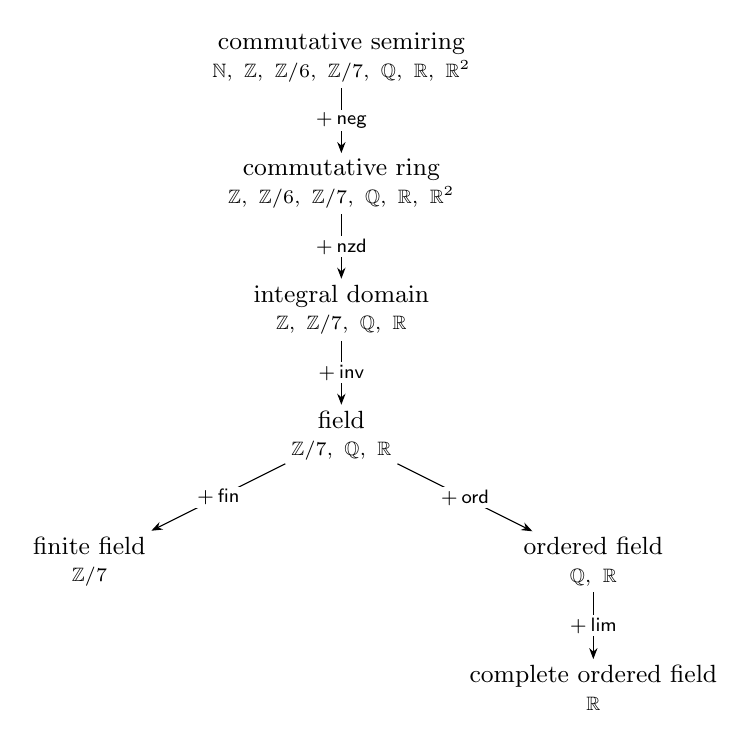
\begin{tikzpicture}[
    x=1cm, y=1cm,
    cls/.style={font=\small, inner sep=2pt, align=center},
    tst/.style={font=\scriptsize, fill=white, inner sep=1pt},
    ar/.style={-{Stealth[length=4pt]}, thin}]
  \node[cls] (S) at (0, 0)     {commutative semiring\\[-1pt]{\scriptsize $\N,\ \Z,\ \Z/6,\ \Z/7,\ \Q,\ \R,\ \R^2$}};
  \node[cls] (R) at (0,-1.6)   {commutative ring\\[-1pt]{\scriptsize $\Z,\ \Z/6,\ \Z/7,\ \Q,\ \R,\ \R^2$}};
  \node[cls] (D) at (0,-3.2)   {integral domain\\[-1pt]{\scriptsize $\Z,\ \Z/7,\ \Q,\ \R$}};
  \node[cls] (F) at (0,-4.8)   {field\\[-1pt]{\scriptsize $\Z/7,\ \Q,\ \R$}};
  \node[cls] (FF) at (-3.2,-6.4) {finite field\\[-1pt]{\scriptsize $\Z/7$}};
  \node[cls] (OF) at (3.2,-6.4)  {ordered field\\[-1pt]{\scriptsize $\Q,\ \R$}};
  \node[cls] (CF) at (3.2,-8.0)  {complete ordered field\\[-1pt]{\scriptsize $\R$}};
  \draw[ar] (S) -- node[tst]{$+\,\mathsf{neg}$} (R);
  \draw[ar] (R) -- node[tst]{$+\,\mathsf{nzd}$} (D);
  \draw[ar] (D) -- node[tst]{$+\,\mathsf{inv}$} (F);
  \draw[ar] (F) -- node[tst]{$+\,\mathsf{fin}$} (FF);
  \draw[ar] (F) -- node[tst]{$+\,\mathsf{ord}$} (OF);
  \draw[ar] (OF) -- node[tst]{$+\,\mathsf{lim}$} (CF);
\end{tikzpicture}
\end{center}


The tests are defined in Chapter 1 of this part: $\mathsf{neg}$ (negatives), $\mathsf{nzd}$ (no zero divisors), $\mathsf{inv}$ (inverses), $\mathsf{fin}$ (finite), $\mathsf{ord}$ (ordered), $\mathsf{lim}$ (limits).

\textbf{How the two floors fit.} On the first floor the dots are systems and each arrow is a chapter. A first-floor chapter moves a system from one class here to another:
\begin{center}
\renewcommand{\arraystretch}{1.3}
\begin{tabular}{@{}l l >{\raggedright\arraybackslash}p{8.2cm}@{}}
\textbf{Chapter of Part I} & \textbf{takes} & \textbf{from class \ $\to$ \ to class} \\ \hline
I.1 & $\N \to \Z$ & semiring \ $\to$ \ integral domain \\
I.2 & $\Z \to \Q$ & integral domain \ $\to$ \ ordered field \\
I.3 & $\Z \to \Z/n$ & integral domain \ $\to$ \ ring, or finite field if $n$ is prime \\
I.4 & $\Q \to \R$ & ordered field \ $\to$ \ complete ordered field \\
I.6 & $\R \to \R^2$ & complete ordered field \ $\to$ \ ring \\
I.7 & $\R \to \R[x]$ & complete ordered field \ $\to$ \ integral domain \\
I.7, road 2 & $\R[x] \to \mathbb{C}$ & integral domain \ $\to$ \ field \\
I.10 & $\R \to C$ & complete ordered field \ $\to$ \ ring \\
\end{tabular}
\end{center}

\textbf{The chapters of Part II.}
\begin{center}
\renewcommand{\arraystretch}{1.3}
{\small
\begin{tabular}{@{}>{\raggedright\arraybackslash}p{4.4cm} >{\raggedright\arraybackslash}p{4.4cm} >{\raggedright\arraybackslash}p{5.6cm}@{}}
\textbf{Chapter} & \textbf{Things} & \textbf{What appears} \\ \hline
II.1 The table & systems and tests & ring, field, complete \\
II.2 Congruences over any ring & one variable row $K$ & ideals; a blur is known by its zero bag \\
II.3 Vector spaces & a second table; one variable row $V$ & subspaces; dimension as a normal form \\
II.4 Metric spaces & a third table; one variable row $X$ & complete, compact; what $\cong_{\mathrm{pt}}$ and $\cong_{\mathrm{u}}$ keep \\
II.5 Modules \emph{(planned)} & one ring acting & ideals and subspaces as one \\
II.6 Arrows \emph{(planned)} & maps between systems & every arrow is a blur, then an inside \\
II.7 One class at a time \emph{(planned)} & one class & theorems true in every row at once \\
II.8 Machines \emph{(planned)} & maps between classes & closing up; the nearest row in a class \\
\end{tabular}
}
\end{center}

\textbf{A second table.} Chapter II.3 changes the operations: $+$ and scaling by reals in place of $+$ and $\times$. Its tests are $\mathsf{add}$, $\mathsf{scale}$ and $\mathsf{findim}$.

\begin{center}
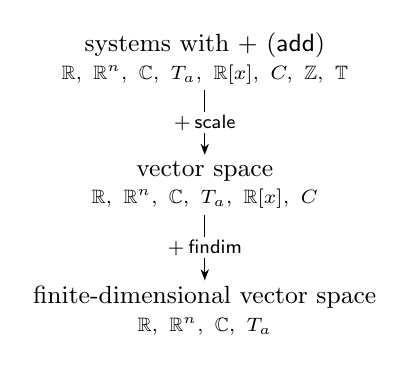
\begin{tikzpicture}[
    x=1cm, y=1cm,
    cls/.style={font=\small, inner sep=2pt, align=center},
    tst/.style={font=\scriptsize, fill=white, inner sep=1pt},
    ar/.style={-{Stealth[length=4pt]}, thin}]
  \node[cls] (A) at (0, 0)   {systems with $+$ ($\mathsf{add}$)\\[-1pt]{\scriptsize $\R,\ \R^n,\ \mathbb{C},\ T_a,\ \R[x],\ C,\ \Z,\ \mathbb{T}$}};
  \node[cls] (V) at (0,-1.6) {vector space\\[-1pt]{\scriptsize $\R,\ \R^n,\ \mathbb{C},\ T_a,\ \R[x],\ C$}};
  \node[cls] (W) at (0,-3.2) {finite-dimensional vector space\\[-1pt]{\scriptsize $\R,\ \R^n,\ \mathbb{C},\ T_a$}};
  \draw[ar] (A) -- node[tst]{$+\,\mathsf{scale}$} (V);
  \draw[ar] (V) -- node[tst]{$+\,\mathsf{findim}$} (W);
\end{tikzpicture}
\end{center}

\textbf{A third table.} Chapter II.4 drops the operations and keeps a distance. Its rows are $\Q$, $\R$, $\R^2$, the two stretches $0 \le x \le 1$ and $0 < x < 1$, the circle $\mathbb{T}$, $C[b,c]$, $\Z$ with the $p$-adic distance $d_p$, $\Z_p$, and $\mathsf{three}$ (three points).

\begin{center}
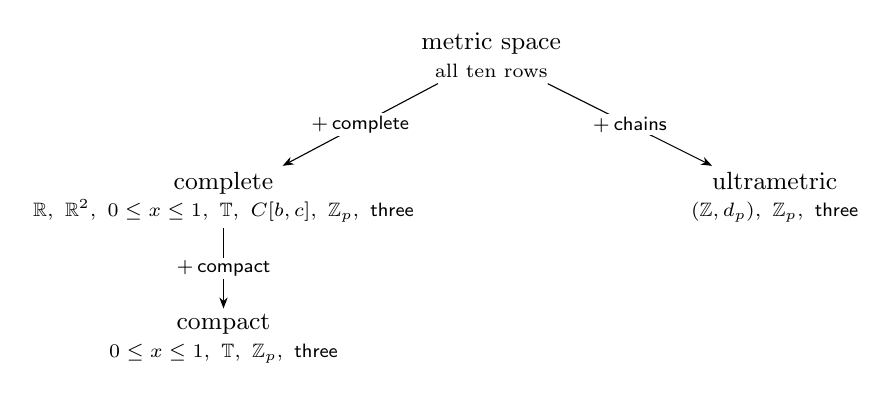
\begin{tikzpicture}[
    x=1cm, y=1cm,
    cls/.style={font=\small, inner sep=2pt, align=center},
    tst/.style={font=\scriptsize, fill=white, inner sep=1pt},
    ar/.style={-{Stealth[length=4pt]}, thin}]
  \node[cls] (M) at (0, 0)      {metric space\\[-1pt]{\scriptsize all ten rows}};
  \node[cls] (C) at (-3.4,-1.8) {complete\\[-1pt]{\scriptsize $\R,\ \R^2,\ 0 \le x \le 1,\ \mathbb{T},\ C[b,c],\ \Z_p,\ \mathsf{three}$}};
  \node[cls] (K) at (-3.4,-3.6) {compact\\[-1pt]{\scriptsize $0 \le x \le 1,\ \mathbb{T},\ \Z_p,\ \mathsf{three}$}};
  \node[cls] (U) at (3.6,-1.8)  {ultrametric\\[-1pt]{\scriptsize $(\Z, d_p),\ \Z_p,\ \mathsf{three}$}};
  \draw[ar] (M) -- node[tst]{$+\,\mathsf{complete}$} (C);
  \draw[ar] (C) -- node[tst]{$+\,\mathsf{compact}$} (K);
  \draw[ar] (M) -- node[tst]{$+\,\mathsf{chains}$} (U);
\end{tikzpicture}
\end{center}
Every compact row is complete (Chapter II.4, T1), so compact sits below complete. $\Z_p$ and $\mathsf{three}$ are in all four classes.

\textbf{Axioms.} None. The Given of Part II is Part I.

\newpage

%% ==================================================================
%%  II.  (p2-ch1-table)
%% ==================================================================
\section*{Chapter II.1. The table}
\phantomsection\addcontentsline{toc}{section}{\texorpdfstring{Chapter II.1. The table \quad systems $\to$ classes}{Chapter II.1. The table}}
\begin{center}
{\normalsize systems $\to$ classes \quad$\cdot$\quad from: all of Part I \quad$\cdot$\quad table, blur, class}\\[4pt]
{\small The things are now the number systems themselves. Forget which system; keep which laws it passes.}
\end{center}

\subsection*{Given}

From Part I, nothing else. (Here ``Chapter I.4'' means Chapter 4 of Part I.)
\begin{lines}
\item[\lab{G1}] (Things.) The systems of Part I: $\N$, $\Z$, $\Q$, $\R$, $\Z/n$ for $n \ge 2$, and $\R^n$ with $+$ and $\ast$. As samples we take $\Z/6$, $\Z/7$ and $\R^2$.
\item[\lab{G2}] (Arrows.) The Arrow lines: $\N \to \Z$, $\Z \to \Q$, $\Q \to \R$ and $\R \to \R^n$ (one-to-one), and $\Z \to \Z/n$ (reaching every bag).
\item[\lab{G3}] (Facts.) The Theorems, Propositions and Exercises of Chapters I.1--I.6, read as yes/no facts about each system.
\end{lines}
In Part I a Given was a list of laws about numbers. Here it is a list of systems, arrows and facts. No new axiom is used.

\subsection*{Definitions}

A \emph{test} is a law that can be asked of a system $K$ with $0$, $1$, $+$, $\times$.
\begin{lines}
\item[\lab{D1}] $\mathsf{semi}$: $+$ and $\times$ are associative and commutative, $0$ and $1$ are neutral, $\times$ distributes over $+$.
\item[\lab{D2}] $\mathsf{neg}$: for every $x$ there is $y$ with $x + y = 0$.
\item[\lab{D3}] $\mathsf{nzd}$: $x \times y = 0 \Rightarrow x = 0$ or $y = 0$.
\item[\lab{D4}] $\mathsf{inv}$: for every $x \neq 0$ there is $y$ with $x \times y = 1$.
\item[\lab{D5}] $\mathsf{ord}$: $K$ has a total order with $x \le y \Rightarrow x + z \le y + z$, and $0 \le x,\, 0 \le y \Rightarrow 0 \le x \times y$.
\item[\lab{D6}] $\mathsf{least}$: $\mathsf{ord}$, and every non-empty set of elements $x > 0$ has a least element.
\item[\lab{D7}] $\mathsf{lim}$: $\mathsf{ord}$, and every sequence that settles has a limit (Chapter I.4, D3 and N3, with $\varepsilon$ in $K$).
\item[\lab{D8}] $\mathsf{dense}$: $\mathsf{ord}$, and if $x < y$ there is $z$ with $x < z < y$.
\item[\lab{D9}] $\mathsf{fin}$: $K$ has finitely many elements.
\item[\lab{D10}] (F3.) For a set $U$ of tests: $K \sim_U L \iff K$ and $L$ give the same answer to every test in $U$.
\item[\lab{D11}] (F4.) For a set $T$ of tests: $\operatorname{class}(T) :=$ the set of systems that pass every test in $T$.
\end{lines}
A test that needs an order counts as failed where there is none.

\subsection*{The table}

\begin{center}
\renewcommand{\arraystretch}{1.3}
\begin{tabular}{l|ccccccccc}
 & $\mathsf{semi}$ & $\mathsf{neg}$ & $\mathsf{nzd}$ & $\mathsf{inv}$ & $\mathsf{ord}$ & $\mathsf{least}$ & $\mathsf{lim}$ & $\mathsf{dense}$ & $\mathsf{fin}$ \\ \hline
$\N$   & $\checkmark$ & $\cdot$ & $\checkmark$ & $\cdot$ & $\checkmark$ & $\checkmark$ & $\checkmark$ & $\cdot$ & $\cdot$ \\
$\Z$   & $\checkmark$ & $\checkmark$ & $\checkmark$ & $\cdot$ & $\checkmark$ & $\checkmark$ & $\checkmark$ & $\cdot$ & $\cdot$ \\
$\Z/6$ & $\checkmark$ & $\checkmark$ & $\cdot$ & $\cdot$ & $\cdot$ & $\circ$ & $\circ$ & $\circ$ & $\checkmark$ \\
$\Z/7$ & $\checkmark$ & $\checkmark$ & $\checkmark$ & $\checkmark$ & $\cdot$ & $\circ$ & $\circ$ & $\circ$ & $\checkmark$ \\
$\Q$   & $\checkmark$ & $\checkmark$ & $\checkmark$ & $\checkmark$ & $\checkmark$ & $\cdot$ & $\cdot$ & $\checkmark$ & $\cdot$ \\
$\R$   & $\checkmark$ & $\checkmark$ & $\checkmark$ & $\checkmark$ & $\checkmark$ & $\cdot$ & $\checkmark$ & $\checkmark$ & $\cdot$ \\
$\R^2$ & $\checkmark$ & $\checkmark$ & $\cdot$ & $\cdot$ & $\cdot$ & $\circ$ & $\circ$ & $\circ$ & $\cdot$ \\
\end{tabular}
\end{center}
$\checkmark$ passes, $\cdot$ fails, $\circ$ cannot be asked (counts as fails). Every entry is a line of Part I or an exercise there.

\subsection*{Blur}

\begin{lines}
\item[\lab{B1}] Choose a set $U$ of tests. The blur is $\sim_U$ (D10): forget which system, keep its answers on $U$.
\item[] Example: $U = \{\mathsf{neg}, \mathsf{inv}\}$ gives three bags: $\{\N\}$, $\ \{\Z, \Z/6, \R^2\}$, $\ \{\Z/7, \Q, \R\}$.
\end{lines}

\subsection*{Propositions}

All of these are read off the table, and were checked by machine.
\begin{lines}
\item[\lab{P1}] (Sharp.) With all nine tests, no two of the seven systems share a bag.
\item[\lab{P2}] (Classes.) As $T$ runs over all sets of tests, $\operatorname{class}(T)$ takes exactly $16$ values.
\item[\lab{P3}] (Arrows as moves.) Each chapter changes one row into another:
\begin{center}
\renewcommand{\arraystretch}{1.2}
\begin{tabular}{lll}
Chapter & gains & loses \\ \hline
I.1. $\N \to \Z$ & $\mathsf{neg}$ & nothing \\
I.2. $\Z \to \Q$ & $\mathsf{inv}$, $\mathsf{dense}$ & $\mathsf{least}$, $\mathsf{lim}$ \\
I.3. $\Z \to \Z/n$ & $\mathsf{fin}$; $\ \mathsf{inv}$ if $n$ is prime & $\mathsf{ord}$, $\mathsf{least}$, $\mathsf{lim}$; $\ \mathsf{nzd}$ unless $n$ is prime \\
I.4. $\Q \to \R$ & $\mathsf{lim}$ & nothing \\
I.6. $\R \to \R^2$ & nothing & $\mathsf{nzd}$, $\mathsf{inv}$, $\mathsf{ord}$, $\mathsf{lim}$, $\mathsf{dense}$ \\
\end{tabular}
\end{center}
\item[\lab{P4}] (In the table.) $\mathsf{inv} \Rightarrow \mathsf{nzd}$; \ $\mathsf{least} \Rightarrow \mathsf{lim}$; \ $\mathsf{dense} \Rightarrow \mathsf{inv}$; \ $\mathsf{inv} \Rightarrow \mathsf{neg}$; \ $\mathsf{fin} \Rightarrow \mathsf{neg}$; \ $\mathsf{ord} \Rightarrow \mathsf{nzd}$.
\item[\lab{P5}] (Never together in the table.) $\mathsf{ord}$ and $\mathsf{fin}$; \ $\mathsf{least}$ and $\mathsf{dense}$; \ $\mathsf{inv}$ and $\mathsf{least}$.
\end{lines}

\subsection*{Appears}

The classes of P2 are what appears. Eight of them have old names.
\begin{lines}
\item[\lab{N1}] $\operatorname{class}(\mathsf{semi})$: all seven. \emph{Commutative semiring.}
\item[\lab{N2}] $\operatorname{class}(\mathsf{semi}, \mathsf{neg})$: $\Z, \Z/6, \Z/7, \Q, \R, \R^2$. \emph{Commutative ring.}
\item[\lab{N3}] $\operatorname{class}(\mathsf{semi}, \mathsf{neg}, \mathsf{nzd})$: $\Z, \Z/7, \Q, \R$. \emph{Integral domain.}
\item[\lab{N4}] $\operatorname{class}(\mathsf{semi}, \mathsf{neg}, \mathsf{inv})$: $\Z/7, \Q, \R$. \emph{Field.}
\item[\lab{N5}] $\operatorname{class}(\mathsf{semi}, \mathsf{neg}, \mathsf{ord})$: $\Z, \Q, \R$. \emph{Ordered ring.}
\item[\lab{N6}] $\operatorname{class}(\mathsf{semi}, \mathsf{neg}, \mathsf{inv}, \mathsf{ord})$: $\Q, \R$. \emph{Ordered field.}
\item[\lab{N7}] $\operatorname{class}(\mathsf{semi}, \mathsf{neg}, \mathsf{inv}, \mathsf{ord}, \mathsf{lim})$: $\R$. \emph{Complete ordered field.}
\item[\lab{N8}] $\operatorname{class}(\mathsf{semi}, \mathsf{neg}, \mathsf{inv}, \mathsf{fin})$: $\Z/7$. \emph{Finite field.}
\end{lines}
None of these words was defined. Each is the name of a set of rows.

The classes and the steps between them are drawn in the map of the second floor, at the start of Part II.

\subsection*{Theorems}

These hold for every system, not only the seven rows. They are stated without proof, like the rest.
\begin{lines}
\item[\lab{T1}] $\mathsf{semi}$ and $\mathsf{inv}$ give $\mathsf{nzd}$.
\item[\lab{T2}] $\mathsf{least}$ gives $\mathsf{lim}$.
\item[\lab{T3}] $\mathsf{least}$ and $\mathsf{dense}$ never hold together.
\item[\lab{T4}] $\mathsf{semi}$, $\mathsf{neg}$, $\mathsf{ord}$ and $\mathsf{fin}$ never hold together, if $0 \neq 1$.
\item[\lab{T5}] (Closing up is ticking a box; F5.) Let $K$ be a system on which the chapter's Definitions and Blur can be carried out with $K$ in place of its Given, and whose Arrow, from $K$ to the new bags, is one-to-one. Call $K$ \emph{closed} for the chapter if that Arrow also reaches every bag. Then:
\begin{gather*}
K \text{ closed for Ch.\,I.1} \iff \mathsf{neg}, \\
K \text{ closed for Ch.\,I.2} \iff \mathsf{inv}, \\
K \text{ closed for Ch.\,I.4} \iff \mathsf{lim}.
\end{gather*}
\item[\lab{T6}] (Once is enough.) The output of Chapter I.1, I.2 or I.4 is closed for that chapter.
\item[\lab{T7}] (Completeness.) So ``complete'' is not a property of $\R$ alone. It is one column of the table, and T5 says the column can be read without mentioning sequences of a particular system: $K$ is complete iff Chapter I.4 has nothing to add to $K$.
\end{lines}

\subsection*{Remarks}

\begin{lines}
\item[\lab{R1}] (The table suggests; new rows refute; F6.) P4 and P5 are facts about seven rows. T1--T4 are the ones that survive every new row. The others are accidents of a small table, and each dies when the right row is added:
\begin{center}
\renewcommand{\arraystretch}{1.2}
\begin{tabular}{ll}
read off the table & a row that breaks it \\ \hline
$\mathsf{dense} \Rightarrow \mathsf{inv}$ & the decimal fractions (Chapter I.2, R3) \\
$\mathsf{inv} \Rightarrow \mathsf{neg}$ & the rationals $x \ge 0$ \\
$\mathsf{fin} \Rightarrow \mathsf{neg}$ & $\{0,1\}$ with $1 + 1 = 1$ \\
$\mathsf{ord}$ and $\mathsf{fin}$ never together & $\{0,1\}$ with $1 + 1 = 1$ \\
\end{tabular}
\end{center}
This is the method's way of finding theorems: read an implication off the table, then either prove it or build the row that kills it.
\item[\lab{R2}] (Blur or class.) $\sim_U$ asks what a set of tests \emph{cannot tell apart}. $\operatorname{class}(T)$ asks what a set of tests \emph{picks out}. Part I used the first. The old names (ring, field) are answers to the second.
\item[\lab{R3}] (Gains and losses.) By P3, Chapters I.1 and I.4 only gain: they are pure closings-up. Chapters I.2 and I.3 trade. Chapter I.6 only loses: building room costs laws. Chapter I.2 loses $\mathsf{lim}$ and Chapter I.4 wins it back.
\item[\lab{R4}] (A small table.) Seven rows cannot show every distinction. A test on which all rows agree is invisible here; so is any class with no row in it.
\end{lines}

\subsection*{Exercises}

\begin{lines}
\item[\lab{E1}] Find the line of Part I behind each entry of the row of $\Q$.
\item[\lab{E2}] List all $16$ classes of P2. Which have no old name? Propose names.
\item[\lab{E3}] Check that $\{0,1\}$ with $1 + 1 = 1$ and the usual $\times$ passes $\mathsf{semi}$, $\mathsf{ord}$ and $\mathsf{fin}$, and add its row to the table. How many classes are there now?
\item[\lab{E4}] $\mathsf{ord} \Rightarrow \mathsf{nzd}$ is in P4 but not among T1--T4. Prove it, or find a row that breaks it.
\item[\lab{E5}] Add the row of the decimal fractions. Which chapters is it closed for?
\end{lines}

\newpage

%% ==================================================================
%%  II.  (p2-ch2-any-ring)
%% ==================================================================
\section*{Chapter II.2. Congruences over any ring}
\phantomsection\addcontentsline{toc}{section}{\texorpdfstring{Chapter II.2. Congruences over any ring \quad $K \to K/I$}{Chapter II.2. Congruences over any ring}}
\begin{center}
{\normalsize $K \to K/I$ \quad$\cdot$\quad from: Chapter II.1, rerunning Chapter I.3 \quad$\cdot$\quad blur}\\[4pt]
{\small Chapter I.3 again, with a class as the Given. See which lines survive.}
\end{center}

\subsection*{Given}

\begin{lines}
\item[\lab{G1}] $K$, any system in $\operatorname{class}(\mathsf{semi}, \mathsf{neg})$: a commutative ring (Chapter II.1, N2).
\end{lines}
Nothing else is known about $K$. Rows to keep in mind: $\Z$, $\Z/6$, $\Z/7$, $\Q$, $\R$, $\R^2$. The floor is $K$ with $O = \{+, \times\}$.

\subsection*{Definitions}

\begin{lines}
\item[\lab{D1}] $-y$ is the $y'$ with $y + y' = 0$ (it is the only one: T1), and $x - y := x + (-y)$.
\item[\lab{D2}] A set $I \subseteq K$ is \emph{closed for $+$} if it holds $0$, holds $x + y$ whenever it holds $x$ and $y$, and holds $-x$ whenever it holds $x$.
\item[\lab{D3}] $I$ is an \emph{ideal} if it is closed for $+$ and holds $k \times x$ whenever it holds $x$, for every $k$ in $K$.
\item[\lab{D4}] For $I$ closed for $+$: \ $x \sim_I y \iff x - y \in I$.
\item[\lab{D5}] For a blur $\sim$ of $K$: its \emph{zero bag} is $\bag{0}$.
\end{lines}

\subsection*{Blur}

\begin{lines}
\item[\lab{B1}] (From below, L5.) Gluings: $g \sim 0$ for every $g$ in a chosen set $G \subseteq K$. \ Respects: $+$, $\times$. \ Call this blur $\sim$. \\
In Chapter I.3, $G = \{n\}$.
\item[\lab{B2}] (From above, L6.) Question: ``is $x$ in $I$?'', for a chosen ideal $I$. \ Respects: $+$, $\times$. \ Call this blur $\approx$.
\end{lines}

\subsection*{Propositions}

\begin{lines}
\item[\lab{P1}] (The zero bag.) If a blur of $K$ respects $+$, its zero bag is closed for $+$. If it also respects $\times$, its zero bag is an ideal.
\item[\lab{P2}] (A blur is known by its zero bag.) If $\sim$ respects $+$, then $x \sim y \iff x - y \in \bag{0}$.
\item[\lab{P3}] (All of them.) $I \mapsto {\sim_I}$ matches the ideals of $K$ one-to-one with the blurs of $K$ respecting $+$ and $\times$. A bigger ideal gives a blurrier blur.
\item[\lab{P4}] (Bags, from below.) The blur B1 is $\sim_I$, where $I$ is the smallest ideal holding $G$: the set of all sums $k_1 g_1 + \dots + k_m g_m$ with $g_i$ in $G$ and $k_i$ in $K$.
\item[\lab{P5}] (Appears.) For every ideal $I$, the blur B2 is $\sim_I$. So every blur of $K$ respecting $+$ and $\times$ is the home of a question, ``is $x$ in $I$?''. \ (By Z4 and Z5; the separating context is $z = -x$.)
\item[\lab{P6}] (Survives.) $+$, $-$ and $\times$ survive $\sim_I$.
\item[\lab{P7}] (Normal forms: lost.) Chapter I.3, P2 used G8 of $\Z$. For a general $K$ there is no rule that picks a member of each bag.
\end{lines}

\subsection*{Notation}

\begin{lines}
\item[\lab{N1}] Let $K/I := K/{\sim_I}$ (M5), with $+$, $-$, $\times$ carried over by P6 (Z6).
\end{lines}

\subsection*{Arrow}

\begin{lines}
\item[\lab{P8}] The map $K \to K/I$, $x \mapsto \bag{x}$, is a picture and respects $0$, $1$, $+$, $\times$.
\item[\lab{P9}] (Every arrow.) If $f : K \to L$ respects $+$ and $\times$, then $I := \{x : f(x) = 0\}$ is an ideal, and $f$ is the picture $K \to K/I$ followed by an inside $K/I \to L$ (W4).
\end{lines}

\subsection*{Theorems}

\begin{lines}
\item[\lab{T1}] (Negatives are unique.) In $K$, if $y + y' = 0$ and $y + y'' = 0$ then $y' = y''$. Also $0 \times x = 0$ for every $x$.
\item[\lab{T2}] (Still a ring.) $K/I$ is in $\operatorname{class}(\mathsf{semi}, \mathsf{neg})$. (All equations: Z7.)
\item[\lab{T3}] (When $\mathsf{nzd}$ holds below.) $K/I$ passes $\mathsf{nzd}$ and has $\bag{0} \neq \bag{1}$ exactly when $I \neq K$ and: $x \times y \in I \Rightarrow x \in I$ or $y \in I$.
\item[\lab{T4}] (When $\mathsf{inv}$ holds below.) $K/I$ passes $\mathsf{inv}$ and has $\bag{0} \neq \bag{1}$ exactly when $I \neq K$ and no ideal lies strictly between $I$ and $K$.
\item[\lab{T5}] (Fields cannot be blurred.) If $0 \neq 1$ in $K$: $K$ passes $\mathsf{inv}$ exactly when its only ideals are $\{0\}$ and $K$. So a field has only the two blurs of Z1.
\item[\lab{T6}] (Chapter I.3 recovered.) For $K = \Z$: every ideal is the set of multiples of exactly one $n \ge 0$. This is where G8 is used, and it is all that is special about $\Z$.
\item[\lab{T7}] (Chapter I.6 recovered.) P1--P3 hold for $\R^n$ with $+$ and scaling in place of $+$ and $\times$: the zero bags are the subspaces. This is I.6, P8.
\end{lines}

\subsection*{Remarks}

\begin{lines}
\item[\lab{R1}] (What survived the change of Given.) Running Chapter I.3 with ``any ring'' in place of $\Z$: the Blur lines, Bags, Survives, Appears and the Arrow survive. Normal forms die (P7). ``$\le$ dies'' has nothing to kill. The theorems on primes turn into T3 and T4, which no longer mention numbers. Reading a proof to see which Given lines it uses is itself a blur: forget the row, keep what the proof needed.
\item[\lab{R2}] (Why $\mathsf{neg}$ earns its column.) P2 fails without negatives. On $\N$, ``$x = y$, or both are $\ge 2$'' is a blur respecting $+$ and $\times$. Its zero bag is $\{0\}$, the same as that of equality. Two blurs, one zero bag.
\item[\lab{R3}] (Twins again.) $\Z/6$ has four ideals, and so has $\R^2$ with $\ast$: nothing, each of the two places, everything. For $\Z/6$ the pictures are $\Z/6$, $\Z/2$, $\Z/3$ and one point. Compare I.6, R2.
\item[\lab{R4}] (Machine check.) For $\Z/6$, $\Z/7$, $\Z/12$ a search over all blurs respecting $+$ and $\times$ finds $4$, $2$, $6$ of them, each with a different zero bag, matching the count of ideals. R2 was checked for all $x, y, z < 30$.
\item[\lab{R5}] (Old names.) T3: prime ideal. T4: maximal ideal. T5: a field is a simple ring. P9: the first isomorphism theorem. $K/I$: quotient ring.
\end{lines}

\subsection*{Exercises}

\begin{lines}
\item[\lab{E1}] Prove P2. (One line in each direction; use that $\sim$ respects $+$.)
\item[\lab{E2}] List the ideals of $\Z/12$ and draw which is inside which. Compare with the divisors of $12$.
\item[\lab{E3}] For each of the four ideals of $\Z/6$, decide T3 and T4.
\item[\lab{E4}] Prove T5. Then explain why Chapter I.2 could not have been followed by a chapter ``congruences on $\Q$''.
\item[\lab{E5}] In R2, find a third blur of $\N$ respecting $+$ and $\times$ with zero bag $\{0\}$.
\end{lines}

\newpage

%% ==================================================================
%%  II.  (p2-ch3-vector-spaces)
%% ==================================================================
\section*{Chapter II.3. Vector spaces}
\phantomsection\addcontentsline{toc}{section}{\texorpdfstring{Chapter II.3. Vector spaces \quad a second table $\to$ one variable row $V$}{Chapter II.3. Vector spaces}}
\begin{center}
{\normalsize a second table $\to$ one variable row $V$ \quad$\cdot$\quad from: Chapters I.6, I.7, I.10, with II.1 and II.2 \quad$\cdot$\quad table, class, blur}\\[4pt]
{\small Many systems of Part I can be added and stretched. Name what they share, then blur any one of them.}
\end{center}

\subsection*{Given}

Part I, and Chapters II.1 and II.2. In this chapter a system has $+$ and, for each real $r$, an operation $x \mapsto r\,x$ called \emph{scaling by $r$}.

\subsection*{A second table}

\begin{lines}
\item[\lab{D1}] $\mathsf{add}$: $+$ is associative and commutative, has a neutral $0$, and every $x$ has a $y$ with $x + y = 0$.
\item[\lab{D2}] $\mathsf{scale}$: the system has a scaling, and for all reals $r, s$: \ $1\,x = x$, \ $(rs)\,x = r\,(s\,x)$, \ $r\,(x + y) = r\,x + r\,y$, \ $(r + s)\,x = r\,x + s\,x$.
\item[\lab{D3}] $\mathsf{findim}$: there is a finite list $x_1, \dots, x_k$ such that every member is $r_1 x_1 + \dots + r_k x_k$ for some reals $r_i$.
\end{lines}

\begin{center}
\renewcommand{\arraystretch}{1.3}
\begin{tabular}{llccc}
\textbf{Row} & \textbf{from} & $\mathsf{add}$ & $\mathsf{scale}$ & $\mathsf{findim}$ \\ \hline
$\R$ & I.4 & yes & yes & yes \\
$\R^n$ & I.6 & yes & yes & yes \\
$\mathbb{C}$ & I.7, road 2 & yes & yes & yes \\
$T_a$, tangent classes & I.11 & yes & yes & yes \\
$\R[x]$ & I.7 & yes & yes & no \\
$C$, continuous maps & I.10 & yes & yes & no \\
$\Z$ & I.1 & yes & no & no \\
$\mathbb{T}$, angles & I.8 & yes & no & no \\
\end{tabular}
\end{center}

\begin{lines}
\item[\lab{P1}] ($\Z$ and $\mathbb{T}$ fail $\mathsf{scale}$.) $\Z$ has no $\tfrac12 \times 1$. In $\mathbb{T}$, scaling died (Chapter I.8, P4.1), and no scaling can be added: $2 \cdot \bag{\tfrac12} = 0$ with $\bag{\tfrac12} \neq 0$, while $\mathsf{scale}$ gives $x = \tfrac12\,(2\,x)$.
\item[\lab{P2}] ($\R[x]$ and $C$ fail $\mathsf{findim}$.) $1, x, x^2, \dots$ are all needed: a finite list of polynomials has a largest degree (Chapter I.7, T2).
\item[\lab{N1}] $\operatorname{class}(\mathsf{add}, \mathsf{scale})$: $\R, \R^n, \mathbb{C}, T_a, \R[x], C$. \emph{Vector space} (over $\R$).
\item[\lab{N2}] $\operatorname{class}(\mathsf{add}, \mathsf{scale}, \mathsf{findim})$: $\R, \R^n, \mathbb{C}, T_a$. \emph{Finite-dimensional vector space.}
\end{lines}

\subsection*{One variable row}

Given $V$, any system in $\operatorname{class}(\mathsf{add}, \mathsf{scale})$.

\subsection*{Definitions}

\begin{lines}
\item[\lab{D4}] A set $W \subseteq V$ is a \emph{subspace} if it holds $0$, and holds $x + y$ and $r\,x$ whenever it holds $x$ and $y$, for every real $r$.
\item[\lab{D5}] For a subspace $W$: \ $x \sim_W y \iff x - y \in W$.
\item[\lab{D6}] The \emph{span} of a set $G$: all sums $r_1 g_1 + \dots + r_m g_m$ with $g_i$ in $G$.
\item[\lab{D7}] A list $x_1, \dots, x_k$ is \emph{independent} if $r_1 x_1 + \dots + r_k x_k = 0$ only when every $r_i = 0$. A \emph{basis} is an independent list whose span is $V$.
\end{lines}

\subsection*{Blur}

\begin{lines}
\item[\lab{B1}] (From below, L5.) Gluings: $g \sim 0$ for every $g$ in a chosen set $G \subseteq V$. \ Respects: $+$ and every scaling. \ Call this blur $\sim$.
\item[\lab{B2}] (From above, L6.) Question: ``is $x$ in $W$?'', for a chosen subspace $W$. \ Respects: $+$ and every scaling. \ Call this blur $\approx$.
\end{lines}

\subsection*{Propositions}

\begin{lines}
\item[\lab{P3}] (The zero bag.) If a blur of $V$ respects $+$ and every scaling, its zero bag is a subspace, and $x \sim y \iff x - y \in \bag{0}$. (As Chapter II.2, P1, P2.)
\item[\lab{P4}] (All of them.) $W \mapsto {\sim_W}$ matches the subspaces of $V$ one-to-one with the blurs of $V$ respecting $+$ and every scaling.
\item[\lab{P5}] (From below.) The blur B1 is $\sim_W$ with $W$ the span of $G$.
\item[\lab{P6}] (Appears.) For every subspace $W$, the blur B2 is $\sim_W$. \ (By Z4 and Z5; the separating context is $z = -x$.)
\item[\lab{P7}] (Survives.) $+$, $-$ and every scaling survive $\sim_W$. (By the choice of $O$.)
\item[\lab{P8}] (Normal forms: by choice.) Chapter II.2, P7 found no normal forms for a general ring. Here there are some, but they must be chosen: if $U$ is a subspace with $U \cap W = \{0\}$ and $U + W = V$, then each bag of $\sim_W$ meets $U$ in exactly one member. Different choices of $U$ give different normal forms.
\end{lines}

\subsection*{Notation}

\begin{lines}
\item[\lab{N3}] $V/W := V/{\sim_W}$ (M5), with $+$ and scaling carried over (Z6). It is again in $\operatorname{class}(\mathsf{add}, \mathsf{scale})$ (Z7: all of D1, D2 are equations, except ``there is a $y$'', which descends from $V$).
\end{lines}

\subsection*{A blur of the rows}

\begin{lines}
\item[\lab{B3}] (On the second floor, F3.) Blur the rows of $\operatorname{class}(\mathsf{add}, \mathsf{scale}, \mathsf{findim})$: glue $V$ and $V'$ when some map $V \to V'$ is one-to-one, reaches every member, and respects $+$ and every scaling.
\item[\lab{T1}] (Bases exist and agree.) Every row of $\operatorname{class}(\mathsf{add}, \mathsf{scale}, \mathsf{findim})$ has a basis, and all its bases have the same length. Call it $\dim V$.
\item[\lab{T2}] (Dimension is the normal form.) $V$ and $V'$ are glued by B3 exactly when $\dim V = \dim V'$. Each bag holds exactly one $\R^n$, namely $n = \dim V$. \ (Chapter I.6, T1 and T5, now for every row.)
\item[\lab{P9}] (In the table.) $\dim \R = 1$, $\dim \R^n = n$, $\dim \mathbb{C} = 2$, $\dim T_a = 2$. So $\mathbb{C}$, $T_a$ and $\R^2$ are glued by B3: as rows of this table they are one. As rows of Chapter II.1 they are not (only $\mathbb{C}$ passes $\mathsf{inv}$). The blur depends on the tests (L7, one floor up).
\end{lines}

\subsection*{Theorems}

\begin{lines}
\item[\lab{T3}] (Dimension of a picture.) If $V$ passes $\mathsf{findim}$ and $W$ is a subspace, then $\dim (V/W) = \dim V - \dim W$.
\item[\lab{T4}] (Subspaces of a finite row.) Every subspace of a finite-dimensional $V$ is finite-dimensional, with $\dim W \le \dim V$, and equality only for $W = V$.
\item[\lab{T5}] (Change of scalars.) Replace $\R$ by any row $K$ of $\operatorname{class}(\mathsf{semi}, \mathsf{neg}, \mathsf{inv})$ of Chapter II.1, the fields. D1--D7, B1--B3, P3--P8 and T1--T4 hold word for word. For $K = \Z/p$, a row of dimension $n$ has exactly $p^n$ members.
\item[\lab{T6}] (The scalars are part of the Given.) $\mathbb{C}$ over $\R$ has dimension $2$; $\mathbb{C}$ over $\mathbb{C}$ (T5 with $K = \mathbb{C}$) has dimension $1$. A row of this table is a system \emph{together with} its scalars.
\end{lines}

\subsection*{Remarks}

\begin{lines}
\item[\lab{R1}] (Why this is not a Part I chapter.) A vector space cannot be built once, the way $\Z$ was. It is a class: a name for what the rows of N1 share. Part I supplied the rows; this chapter only names them and blurs them.
\item[\lab{R2}] (Twins.) Chapter II.2: rings, ideals, quotient rings, no normal forms. This chapter: vector spaces, subspaces, quotient spaces, normal forms by choice. The lines are the same; only the operations in $O$ differ. Chapter II.2, T7 already saw this for $\R^n$.
\item[\lab{R3}] (Why the class is needed.) If every row were some $\R^n$, T2 would make the name unnecessary. $\R[x]$ and $C$ fail $\mathsf{findim}$, and they are where most of analysis lives. They are the reason for N1.
\item[\lab{R4}] (Infinite bases.) $\R[x]$ has a basis without end: $1, x, x^2, \dots$ (with sums of finitely many terms). Whether $C$ has a basis cannot be settled with M1--M7: it needs a rule of choice, which is not in Chapter 0.
\item[\lab{R5}] (What comes next.) Maps between rows that respect $+$ and scaling are the linear maps. Their kernels are zero bags (P3), and ``every arrow is a blur, then an inside'' with T3 gives rank plus nullity. That is the chapter on Arrows, II.6.
\item[\lab{R6}] (Machine check.) For $(\Z/2)^2$, $(\Z/3)^2$, $(\Z/2)^3$, a search over all partitions finds $5$, $6$, $16$ blurs respecting $+$ and every scaling, each with a different zero bag, and each zero bag a subspace: the count of subspaces (\texttt{p2-ch3-check.py}).
\item[\lab{R7}] (Old names.) P4: subspaces are the congruences of a vector space. P8: complements. T1: the dimension theorem. T2: classification of finite-dimensional spaces. B3: isomorphism.
\end{lines}

\subsection*{Exercises}

\begin{lines}
\item[\lab{E1}] Check $\mathsf{scale}$ for $C$. Which part of Chapter I.10 shows $C$ is closed under scaling?
\item[\lab{E2}] In $\R^2$, let $W$ be the line through $0$ and $(1,1)$. Give two different complements $U$ and the normal form of the bag of $(3, 5)$ for each.
\item[\lab{E3}] Show that the polynomials $p$ with $p(2) = 0$ form a subspace $W$ of $\R[x]$. What is $\R[x]/W$? (Hint: Chapter I.7, road 1.)
\item[\lab{E4}] List the five subspaces of $(\Z/2)^2$ and draw which is inside which.
\item[\lab{E5}] Prove P1's claim that $\mathbb{T}$ admits no scaling.
\item[\lab{E6}] Find a basis of $T_a$ and the map that glues it to $\R^2$ by B3.
\end{lines}

\newpage

%% ==================================================================
%%  II.  (p2-ch4-metric-spaces)
%% ==================================================================
\section*{Chapter II.4. Metric spaces}
\phantomsection\addcontentsline{toc}{section}{\texorpdfstring{Chapter II.4. Metric spaces \quad systems with a distance $\to$ classes}{Chapter II.4. Metric spaces}}
\begin{center}
{\normalsize systems with a distance $\to$ classes \quad$\cdot$\quad from: Chapters I.4, I.5, I.8, I.10, I.18, I.19, I.20 \quad$\cdot$\quad table, class, blur}\\[4pt]
{\small Part I met a distance five times. Put the five side by side, read the classes off the table, and ask which tests survive when two rows are glued by an arrow.}
\end{center}

\subsection*{Given}

Part I, and Chapter II.1. In this chapter a system is a bag $X$ with a map $d : X \times X \to \R$, its \emph{distance}. There are no operations.

\subsection*{The rows}

\begin{center}
\renewcommand{\arraystretch}{1.3}
{\small
\begin{tabular}{@{}>{\raggedright\arraybackslash}p{5.6cm} >{\raggedright\arraybackslash}p{6.4cm} l@{}}
\textbf{Row} & \textbf{distance} & \textbf{from} \\ \hline
$\Q$, \ $\R$ & $|x - y|$ & I.2, I.4 \\
$\R^2$ & $|x - y|$ of I.13, D1 & I.6, I.13 \\
the stretch $0 \le x \le 1$; \ the open stretch $0 < x < 1$ & $|x - y|$ & I.10, D8 \\
the circle $\mathbb{T}$ & $d$ of I.8, T5 & I.8 \\
$C[b,c]$ & largest gap: $\max |f(x) - g(x)|$ on the stretch & I.20 \\
$(\Z, d_p)$: \ $\Z$ with the $p$-adic distance & $d_p(x, y) := p^{-v_p(x - y)}$, and $0$ when $x = y$ & I.18, D4 \\
$\Z_p$ & $p^{-m}$ when $x - y = p^m u$, $u$ with an inverse & I.19, T3 \\
$\mathsf{three}$: three points & $1$ between any two & --- \\
\end{tabular}
}
\end{center}

\subsection*{Tests}

Each row has its nearness: $x \mathrel{N_k} y$ iff $d(x, y) < 10^{-k}$, with $\operatorname{near}_k(x)$, ``comes near'' and ``comes near itself'' as in Chapter I.5, N2 and N5.
\begin{lines}
\item[\lab{D1}] $\mathsf{dist}$: \ $d(x, y) \ge 0$; \ $d(x, y) = 0$ only for $x = y$; \ $d(x, y) = d(y, x)$; \ $d(x, z) \le d(x, y) + d(y, z)$.
\item[\lab{D2}] $\mathsf{complete}$: every sequence that comes near itself comes near some member.
\item[\lab{D3}] $\mathsf{bounded}$: there is a real $B$ with $d(x, y) \le B$ for all $x, y$.
\item[\lab{D4}] $\mathsf{compact}$: every sequence has a part $a_{i_0}, a_{i_1}, \dots$ ($i_0 < i_1 < \dots$) that comes near some member.
\item[\lab{D5}] $\mathsf{onepiece}$: the row cannot be cut: every blur $\sim$ of $X$ such that each $x$ has a rung $k$ with $\operatorname{near}_k(x) \subseteq \bag{x}$ has one bag (as in Chapter I.5, T1).
\item[\lab{D6}] $\mathsf{chains}$: \ $d(x, z) \le \max\bigl(d(x, y),\ d(y, z)\bigr)$. Then every $N_k$ is a blur.
\end{lines}

\subsection*{The table}

\begin{center}
\renewcommand{\arraystretch}{1.3}
{\small
\setlength{\tabcolsep}{5pt}
\begin{tabular}{l|cccccc}
 & $\mathsf{dist}$ & $\mathsf{complete}$ & $\mathsf{bounded}$ & $\mathsf{compact}$ & $\mathsf{onepiece}$ & $\mathsf{chains}$ \\ \hline
$\Q$ & $\checkmark$ & $\cdot$ & $\cdot$ & $\cdot$ & $\cdot$ & $\cdot$ \\
$\R$ & $\checkmark$ & $\checkmark$ & $\cdot$ & $\cdot$ & $\checkmark$ & $\cdot$ \\
$\R^2$ & $\checkmark$ & $\checkmark$ & $\cdot$ & $\cdot$ & $\checkmark$ & $\cdot$ \\
$0 \le x \le 1$ & $\checkmark$ & $\checkmark$ & $\checkmark$ & $\checkmark$ & $\checkmark$ & $\cdot$ \\
$0 < x < 1$ & $\checkmark$ & $\cdot$ & $\checkmark$ & $\cdot$ & $\checkmark$ & $\cdot$ \\
$\mathbb{T}$ & $\checkmark$ & $\checkmark$ & $\checkmark$ & $\checkmark$ & $\checkmark$ & $\cdot$ \\
$C[b,c]$ & $\checkmark$ & $\checkmark$ & $\cdot$ & $\cdot$ & $\checkmark$ & $\cdot$ \\
$(\Z, d_p)$ & $\checkmark$ & $\cdot$ & $\checkmark$ & $\cdot$ & $\cdot$ & $\checkmark$ \\
$\Z_p$ & $\checkmark$ & $\checkmark$ & $\checkmark$ & $\checkmark$ & $\cdot$ & $\checkmark$ \\
$\mathsf{three}$ & $\checkmark$ & $\checkmark$ & $\checkmark$ & $\checkmark$ & $\cdot$ & $\checkmark$ \\
\end{tabular}
}
\end{center}

Where each entry comes from:
\begin{lines}
\item[\lab{P1}] ($\mathsf{complete}$.) $\Q$ fails: the decimals of $\sqrt2$ (I.4, E3). $\R$: I.4, T6; $\R^2$ place by place. $0 \le x \le 1$ passes, $0 < x < 1$ fails ($1/n$). $\mathbb{T}$ passes (a picture of $\R$, I.8). $C[b,c]$: I.20, T1. $(\Z, d_p)$ fails: the sums $1 - p + p^2 - \dots \pm p^i$ come near themselves, and in $\Z_p$ they come near the inverse of $1 + p$ (as in I.19, T2: $(1 + p)$ times the $i$-th sum is $1 \pm p^{i+1}$), which is not in $\Z$. (The sums of I.19, T2 will not do for $p = 2$: there $1/(1 - p) = -1$ is in $\Z$.) $\Z_p$: I.19, T10. $\mathsf{three}$: a sequence that comes near itself is eventually constant.
\item[\lab{P2}] ($\mathsf{bounded}$, $\mathsf{compact}$.) $\R$, $\R^2$, $C[b,c]$ hold the constants $0, 1, 2, \dots$, which no part of brings near anything. $0 \le x \le 1$ is compact (from I.4, T8, halving); $\mathbb{T}$ is its picture. $\Z_p$: halving becomes ``choose a digit that occurs infinitely often'', $p$ choices at each rung. $\mathsf{three}$: some point occurs infinitely often. $0 < x < 1$ and $(\Z, d_p)$ fail by the sequences of P1.
\item[\lab{P3}] ($\mathsf{onepiece}$.) $\R$: I.5, T1; the same proof serves $\R^2$, both stretches, $\mathbb{T}$ and $C[b,c]$ (join any two members by the straight path $f + t(g - f)$, $0 \le t \le 1$). $\Q$ is cut at $\sqrt2$ (I.5, E6). The three rows that chain are cut by T2 below.
\item[\lab{P4}] ($\mathsf{chains}$.) $(\Z, d_p)$ and $\Z_p$: I.19, P2. $\mathsf{three}$: $1 \le \max(1, 1)$. The other rows fail with $0$, $\tfrac12$, $1$ (on $\mathbb{T}$: $0$, $\tfrac14$, $\tfrac12$; on $C[b,c]$: the constants).
\end{lines}

\subsection*{Appears}

\begin{lines}
\item[\lab{N1}] $\operatorname{class}(\mathsf{dist})$: every row. \emph{Metric space.}
\item[\lab{N2}] $\operatorname{class}(\mathsf{dist}, \mathsf{complete})$: $\R$, $\R^2$, $0 \le x \le 1$, $\mathbb{T}$, $C[b,c]$, $\Z_p$, $\mathsf{three}$. \emph{Complete metric space.}
\item[\lab{N3}] $\operatorname{class}(\mathsf{dist}, \mathsf{compact})$: $0 \le x \le 1$, $\mathbb{T}$, $\Z_p$, $\mathsf{three}$. \emph{Compact metric space.}
\item[\lab{N4}] $\operatorname{class}(\mathsf{dist}, \mathsf{chains})$: $(\Z, d_p)$, $\Z_p$, $\mathsf{three}$. \emph{Ultrametric space.} The rows where a ladder of true blurs is enough (I.19), against the rows where likeness is needed (I.5).
\end{lines}

\subsection*{Theorems}

These hold for every row, not only the ten.
\begin{lines}
\item[\lab{T1}] $\mathsf{compact}$ gives $\mathsf{complete}$ and $\mathsf{bounded}$.
\item[\lab{T2}] (Chaining cuts.) A row with at least two points that passes $\mathsf{chains}$ fails $\mathsf{onepiece}$. \ (Take $x \neq y$ and $r := d(x, y)$. ``$d(u, v) < r$'' is a blur, by $\mathsf{chains}$; each of its bags holds $\operatorname{near}_k$ of each of its points once $10^{-k} \le r$; and $x$, $y$ lie in different bags.)
\end{lines}

\subsection*{One variable row $X$}

Fix a row $X$ that passes $\mathsf{dist}$.
\begin{lines}
\item[\lab{P5}] (Its nearness.) The rungs $N_k$ are a nearness (I.5, D4): nested, two steps for one by the triangle law, and the bottom is equality. ``Respects nearness'' for a map between two rows is I.5, N4, with the rungs of each row on its side.
\item[\lab{D7}] (Run Chapter I.4 on $X$.) Build sequences in $X$ (M2); select those that come near themselves (M4); glue $a \sim b$ when $d(a_i, b_i)$ comes near $0$. \ Respects: nothing ($X$ has no operations). Here the gluing is the bag test. Call the bags $\widehat X$, with $d(\bag{a}, \bag{b}) :=$ the limit of $d(a_i, b_i)$.
\item[\lab{T3}] (The closing-up is closed, F5.) $\widehat X$ passes $\mathsf{dist}$ and $\mathsf{complete}$. The arrow $X \to \widehat X$, $x \mapsto \bag{(x, x, \dots)}$, is one-to-one and keeps $d$. Running D7 on $\widehat X$ gives nothing new. $X$ passes $\mathsf{complete}$ iff the arrow also reaches every bag.
\item[\lab{T4}] (Three closings-up from Part I.) $\widehat{\Q} = \R$ (I.4). $\widehat{(\Z, d_p)} = \Z_p$ (I.19). For the polynomials, read as maps on a stretch with the largest gap: $\widehat{\ } = C[b,c]$ (I.20, R4; classical, Weierstrass, long, not proved here).
\item[\lab{T5}] (Contraction; Chapter 25, T2 is the case of a closed box.) If $X$ passes $\mathsf{complete}$, and $f : X \to X$ has $d(f(x), f(y)) \le q\, d(x, y)$ for a fixed $q < 1$, then exactly one $x$ has $f(x) = x$, and from any start, $x_0$, $f(x_0)$, $f(f(x_0))$, \dots comes near it. \\
Examples: $\cos$ on $0 \le x \le 1$ ($q = \sin 1$); \ $x \mapsto p x + 1$ on $\Z_p$ ($q = 1/p$), whose fixed point is $1/(1 - p)$ of I.19, T2.
\end{lines}

\subsection*{Blur: glue two rows by an arrow}

\begin{lines}
\item[\lab{D8}] $X \cong_{\mathrm{pt}} Y$: there is a map $h : X \to Y$, one-to-one and onto, such that $h$ and its inverse respect nearness \emph{at each point}.
\item[\lab{D9}] $X \cong_{\mathrm{u}} Y$: the same, with $h$ and its inverse respecting nearness \emph{with one rung for all points}.
\item[\lab{P6}] Both are blurs on rows (identity; inverse; composing, I.5, T4). $\cong_{\mathrm{u}}$ is less blurry than $\cong_{\mathrm{pt}}$.
\item[\lab{P7}] (Under $\cong_{\mathrm{pt}}$: $\mathsf{compact}$ and $\mathsf{onepiece}$ survive; $\mathsf{complete}$ dies.) \\
Witness: $h(x) = 1/(1 + \exp(-x))$ from $\R$ onto $0 < x < 1$, with inverse $t \mapsto L\bigl(t/(1 - t)\bigr)$ (I.10, T3, T5; I.11, T4; I.12, T5). Both respect nearness at each point. $\R$ passes $\mathsf{complete}$; $0 < x < 1$ fails it. The same witness kills $\mathsf{bounded}$.
\item[\lab{P8}] (Under $\cong_{\mathrm{u}}$: $\mathsf{complete}$ survives too.) A map that respects nearness with one rung for all points sends a sequence that comes near itself to one that comes near itself. Apply this to $h$ and to its inverse. \\
In P7, $h$ respects nearness with one rung, but its inverse does not: near $t = 0$, the inputs $t$ and $t/2$ come near each other while their outputs stay $L(2)$ apart.
\item[\lab{P9}] (Under $\cong_{\mathrm{u}}$: $\mathsf{bounded}$ and $\mathsf{chains}$ still die.) $\R$ with $|x - y|$ and $\R$ with $\min(|x - y|, 1)$ are glued by the identity; one is bounded, one is not. $\mathsf{three}$ and the three points with distances $1, 1, \tfrac32$ are glued by the identity (at rung $1$ both nearnesses are equality); one chains, one does not.
\item[\lab{P10}] (What the three blurs see.) $\mathsf{compact}$ and $\mathsf{onepiece}$ are questions about nearness at points. $\mathsf{complete}$ is a question about nearness with one rung for all points. $\mathsf{bounded}$ and $\mathsf{chains}$ are questions about the numbers $d(x, y)$ themselves, and those numbers die as they did in I.5, P15.
\end{lines}

\subsection*{Remarks}

\begin{lines}
\item[\lab{R1}] (The table suggests; a new row refutes; F6.) In the table, every row that is $\mathsf{complete}$ and $\mathsf{bounded}$ is $\mathsf{compact}$. That is an accident of ten rows. The row $\N$ with distance $1$ between any two different members is complete (a sequence that comes near itself is eventually constant) and bounded, and $0, 1, 2, \dots$ has no part that comes near anything.
\item[\lab{R2}] (Why this chapter is Part II.) The tests ask about every sequence of a row, so they are laws about rows, as in II.1. The rows were built in Part I; this chapter only puts them side by side (F7).
\item[\lab{R3}] (No normal form.) No rule picks one row from each bag of $\cong_{\mathrm{pt}}$ or $\cong_{\mathrm{u}}$.
\item[\lab{R4}] (Old names.) $\mathsf{dist}$: metric. $\mathsf{onepiece}$: connected. $\mathsf{chains}$: ultrametric. $\widehat X$: the completion. T5: Banach's fixed point theorem. $\cong_{\mathrm{pt}}$: homeomorphic; $\cong_{\mathrm{u}}$: uniformly homeomorphic. P10: topological against uniform properties.
\item[\lab{R5}] (Machine check.) Only a little of this chapter can be checked by machine: the finite rows (P4, P9), the $p$-adic triangle law with $\max$ for $p = 2, 3, 5$, the sequence of P1 for $p = 2, 3$, both examples of T5, and the witness of P7 and P8 numerically (\texttt{p2-ch4-check.py}). Everything else rests on the cited lines.
\end{lines}

\subsection*{Exercises}

\begin{lines}
\item[\lab{E1}] Check $\mathsf{dist}$ for the largest gap on $C[b,c]$.
\item[\lab{E2}] Show that $\mathsf{three}$ fails $\mathsf{onepiece}$ by writing down a blur with two bags.
\item[\lab{E3}] Prove T1: if a sequence comes near itself and a part of it comes near $x$, the whole sequence comes near $x$.
\item[\lab{E4}] Add the row $\N$ of R1 to the table. Which classes of N1--N4 does it join?
\item[\lab{E5}] Show that $h$ of P7 respects nearness with one rung for all points. (Hint: its slope is at most $\tfrac14$; Chapter I.11, T6.)
\item[\lab{E6}] Find the fixed point of $x \mapsto 2x + 1$ in $\Z_2$, and its last six digits.
\end{lines}

\end{document}
